\documentclass[a4paper,12pt]{report}

% lingua
\usepackage[italian]{babel}

%titoli capitoli 
\usepackage{titlesec}

% encoding
\usepackage[utf8]{inputenc}
\usepackage[T1]{fontenc}

% matematica
\usepackage{amsmath}
\usepackage{amssymb}
\usepackage{amsthm}
\usepackage{mathtools}
\usepackage{mathrsfs} %il comando è \mathscr{}

% grafica
\usepackage{graphicx}
\everymath{\displaystyle}
\usepackage{xcolor}
\usepackage{float}
\usepackage{tocloft}
\usepackage{fancyhdr}
\pagestyle{fancy}

\fancyhf{}

\makeatletter
\setlength{\headwidth}{\dimexpr\textwidth+\marginparsep+\marginparwidth\relax}
\makeatother

\renewcommand{\chaptermark}[1]{%
\markboth{Capitolo \thechapter: #1}{}}

\renewcommand{\sectionmark}[1]{%
\markright{#1}}

\fancyhead[LE]{Appunti di Metodi Matematici 1}
\fancyhead[RO]{\nouppercase{\leftmark\ifx\rightmark\empty\else\ -- \rightmark\fi}}

\fancyfoot[C]{\thepage}

\renewcommand{\headrulewidth}{1pt}
%sottolineature 
\usepackage{soul}

% link cliccabili
\usepackage{hyperref}

% margini
\usepackage[a4paper,margin=2.5cm]{geometry}

% ambienti matematici
\newtheorem{teorema}{Teorema}[chapter] 
\newtheorem{definizione}{Definizione}[chapter]
\newtheorem{algoritmo}{Algoritmo}[chapter]
\newtheorem{proposizione}{Proposizione}[chapter]
\newtheorem{lemma}{Lemma}[chapter]
\newtheorem{corollario}{Corollario}[chapter]

% comandi utili
\newcommand{\R}{\mathbb{R}}
\newcommand{\norm}[1]{\left\| #1 \right\|}
\newcommand{\lt}{<}
\newcommand{\gt}{>}
\newcommand{\pd}[2]{\frac{\partial #1}{\partial #2}}
\newcommand{\pdd}[2]{\frac{\partial^2 #1}{\partial #2^2}}
\newcommand{\pdm}[3]{\frac{\partial^2 #1}{\partial #2 \partial #3}}




\titleformat{\chapter}[hang]   % stile hang (numero + titolo sulla stessa riga)
  {\normalfont\huge\bfseries} % formato del testo
  {Capitolo \thechapter:}      % etichetta numerica
  {0pt}                        % distanza tra numero e titolo
  {}                            % codice prima del titolo








\begin{document}


\begin{titlepage}

\centering

\vspace*{3cm}
{\fontsize{31}{40}\selectfont\bfseries Appunti di Metodi Matematici 1\par}

\vspace*{0.5cm}
{\Large\bfseries Filippo Arena\par}

\vspace*{2cm}
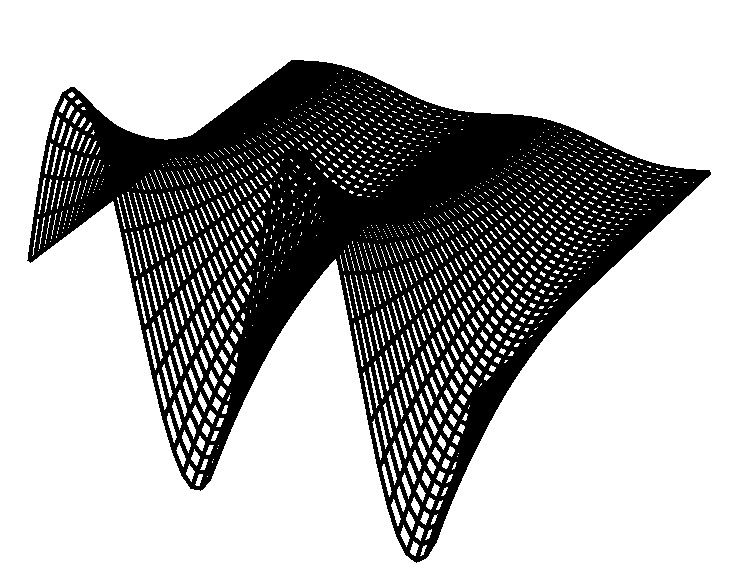
\includegraphics[width=1\linewidth]{Figure_2_cropped.pdf}

\end{titlepage}

\newpage
\thispagestyle{empty}
\newpage

\null

\chapter*{Introduzione}

Queste dispense nascono con l’obiettivo di fornire un materiale prevalentemente teorico, il più possibile completo e autoconsistente, utile alla preparazione dell’esame di Metodi Matematici 1 del corso di laurea triennale in Fisica dell’Università di Pisa. I contenuti derivano in larga parte dagli appunti delle lezioni dell’omonimo corso, tenute nel secondo semestre dell’anno accademico 2025-26 dal Professor Stefano Bolognesi, nonché dal materiale didattico disponibile sulla pagina e-learning del corso e da ulteriori fonti, che saranno opportunamente citate in bibliografia.
\\Nel seguito verranno trattati argomenti appartenenti alla branca dell’analisi funzionale, di grande rilevanza per un percorso di studi in Fisica. Per questo motivo, alcuni concetti ritenuti meno centrali non saranno approfonditi in modo esaustivo e il linguaggio adottato, pur rimanendo formale, sarà più vicino a quello del fisico che a quello del matematico.
\\Per una piena comprensione degli argomenti è richiesta una solida conoscenza dell’algebra lineare e dei corsi di Analisi 1 e 2. L’obiettivo principale di questa disciplina è infatti quello di fornire il linguaggio matematico necessario allo studio di numerosi ambiti della Fisica, dalla descrizione dei fenomeni ondulatori fino alla meccanica quantistica.
\\Qualora il lettore dovesse imbattersi in imprecisioni, spiegazioni poco chiare o errori tipografici, è invitato a segnalarli, così da poter migliorare il testo e renderne più chiara l’esposizione.
\\Infine, si desidera sottolineare che queste dispense non intendono in alcun modo sostituire la partecipazione alle lezioni e alle esercitazioni: oltre al fatto che alcuni argomenti potrebbero differire, il confronto diretto con il docente rimane comunque un elemento importante per una comprensione più solida degli argomenti.
\\
\\Buona lettura.

\clearpage
\vspace*{-2cm}
\tableofcontents
\fancyhead[RO]{Indice}
\newpage
\thispagestyle{empty}
\newpage

\fancyhead[RO]{\nouppercase{\leftmark\ -- \rightmark}}
\chapter{\ Richiami}

In questo primo capitolo riprenderemo rapidamente alcuni concetti di analisi e algebra lineare (molti dei quali verranno nuovamente affrontati in contesti diversi nei capitoli successivi), indispensabili per la trattazione degli argomenti successivi. Verrà inoltre introdotta la notazione utilizzata nel seguito.
\\Il capitolo potrà risultare piuttosto arido dal punto di vista espositivo e talvolta dare l’impressione di una semplice sequenza di definizioni e teoremi. Questo dipende sia dalla natura di richiamo dei contenuti, sia dal fatto che tali elementi serviranno nei capitoli successivi come riferimento rapido per avere sempre a disposizione definizioni e risultati fondamentali.

\section{Algebra Lineare}\label{sec: 1.1}

Rivediamo alcune definizioni e proprietà inerenti alla teoria degli spazi vettoriali.
\begin{definizione}[Spazio vettoriale]
    Fissato un campo $\mathbb{K}$ (useremo quasi prevalentemente i campi $\mathbb{R}$ e $\mathbb{C}$) definiamo lo spazio vettoriale come l'insieme V di elementi detti vettori dotati di due operazioni binarie quali $\textbf{somma}$ che associa a v,w $\in$ V un elemento (v+w) $\in$ V, e $\textbf{prodotto per scalare}$ che associa a un v $\in$ V e un $\lambda \in \mathbb{K}$ un elemento $\lambda v \in$ V.
    Tali operazioni devono soddisfare le seguenti prorpietà:
    \\
    \\ 1)L'insieme V è un gruppo commutativo con la somma + 
    \\ 2)$\lambda(v+w)= \lambda v+ \lambda w$ 
    \\ 3)$( \lambda+ \mu)v= \lambda v + \mu v$
    \\ 4)$(\lambda \mu)v=\lambda (\mu v)$
    \\ 5)$1v=v$
    \\
    \\Dove $v,w \in V$ e $\lambda, \mu \in \mathbb{K}$.
\end{definizione}
\begin{definizione}[Indipendenza lineare]
    Diremo che i vettori $v_1,v_2,...,v_n\in V$ sono linearmente indipendenti $\iff \displaystyle \sum_{i=1}^{n}\lambda_i v_i =0 \implies \lambda_i=0 \ \forall i \in \{1,..,n\}$ con $\lambda_i \in \mathbb{K}$. 
    \\Se $\exists$ un $\lambda_j \neq 0$ significa che $v_j$ può essere scritto come combinazione lineare degli altri vettori e quindi non ho più l'indipendenza lineare.
\end{definizione}
\begin{definizione}[Dimensione]
    La dimensione di uno spazio vettoriale $V$ è il massimo numero di vettori linearmente indipendenti che vivono in tale spazio. La dimensione di uno spazio vettoriale dipende anche dal campo su cui è definito tale spazio. Ad esempio se prendiamo $V=\mathbb{C}^n$ avremo che $dim_{\mathbb{C}}(\mathbb{C}^n)=n$ mentre $dim_{\mathbb{R}}(\mathbb{C}^n)=2n$ poichè in $\mathbb{R}$ ogni elemento appartenente a $\mathbb{C}$ è identificato da due elementi di $\mathbb{R}$.
\end{definizione}

\newpage

\begin{definizione}[Sottospazio]
    Dato uno spazio vettoriale $V$ definiamo $W \subset V$ sottospazio di $V$ se valgono le seguenti proprietà:
    \\
    \\1) $\forall w_1,w_2 \in W \implies w_1+w_2 \in W$
    \\2) $\forall w\in W,\forall\lambda\in \mathbb{K} \implies \lambda w \in W$
    \\
    \\Notiamo anche che dalla seconda proprietà discende $0 \in W$ dove $0$ è l'elemento neutro dello spazio $V$ di partenza.
\end{definizione}

\subsection{Basi}

\begin{definizione}[Base di uno spazio vettoriale]
    Preso uno spazio vettoriale $V$ con $dim_{\mathbb{K}}(V)=n$, definiamo base di $V$ un insieme ordinato di $v_1,...,v_n \in V$ linearmente indipendenti che generino lo spazio (quindi che soddisfino la relazione $Span(v_1,...,v_n)=V$) e la indicheremo come $B_V=\{v_1,...,v_n\}.$
\end{definizione}

\textbf{\underline{Nota}}: Solitamente, quando si scrive un elenco di elementi tra parentesi graffe si intende un insieme di elementi non ordinati, mentre per un elenco ordinato si usano le tonde. Per non rendere la notazione eccessivamente pesante gli elementi della base verranno scritti tra parentesi graffe tenendo però a mente che due basi formate dagli stessi vettori disposti in ordine diverso sono due basi diverse.
\\
\\
Dalla definizione segue che uno spazio vettoriale può avere diverse basi e gli elementi che lo compongono (anche se rimangono intrinsecamente gli stessi) si scrivono in modo diverso a seconda della base utilizzata. Se prendiamo $B_V=\{v_1,...,v_n\}$ come base di $V$ allora un generico $w \in V$ si scriverà come $w=(\mu_1,...,\mu_n)$ dove i coefficienti $\mu_i\in \mathbb{K}$ sono gli scalari che ci permettono di rappresentare $w$ come combinazione lineare dei vettori di base, quindi $\displaystyle w=\sum_{i=1}^{n}\mu_iv_i$.
\\
Notiamo anche che se prendiamo solo alcuni dei vettori che costituiscono la base del nostro spazio $V$ questi genereranno uno spazio $W$ con  $dim_{\mathbb{K}}(W) < dim_{\mathbb{K}}(V)$ contenuto in $V$. Si dimostra facilmente che $W$ è sottospazio di $V$ verificando la validità delle proprietà 1 e 2 dei sottospazi vettoriali.

\begin{definizione}[Base canonica]
    La base canonica è la base più semplice che possiamo scegliere. Preso $\mathbb{R}^n$ spazio vettoriale con $dim(V)=n$ definiamo come base canonica le n-uple $v_1=(1,0,0,...,0), v_2=(0,1,0,...,0),..., v_n=(0,0,0,...,1)$. Generalmente la base canonica (per qualsiasi spazio vettoriale si indica con laseguente notazione: 
    \\$B(\mathbb{R}^n)=\{e_1,e_2,...,e_n\}$. 

\end{definizione}
È possibile definire la base canonica anche per spazi vettoriali differenti da $\mathbb{R}^n$. Ad esempio lo spazio dei polinomi a coefficienti in $\mathbb{R}$ di grado $n$ arbitrario ha come base canonica $B(\mathbb{R}_n[x])=\{1, x,x^2,...,x^n\}$. 
\\Un'altra base canonica di uno spazio vettoriale che ricorre frequentemente è quello delle
\\
\\matrici quadrate a coefficienti in $\mathbb{R}$, $B(M_2(\mathbb{R}))=\left\{ \begin{pmatrix}
    1 & 0 \\0 & 0
\end{pmatrix},\begin{pmatrix}
    0 & 1 \\0 &0
\end{pmatrix},\begin{pmatrix}
    0 &0 \\ 1 &0
\end{pmatrix},\begin{pmatrix}
    0 & 0\\ 0 &1
\end{pmatrix}\right\}$.


\newpage


\subsection{Applicazioni lineari}

\begin{definizione}[Applicazione lineare]
    Dati due spazi vettoriali $V$ e $W$ definiamo applicazione lineare una funzione $A:V\to W$ che preserva la struttura lineare, in altri termini $A(\lambda v+\mu w)=\lambda A(v)+\mu A(w) \ \ \forall v,w \in V, \forall \lambda, \mu \in \mathbb{K}$.
\end{definizione}

 Come tutte le funzioni le applicazioni lineari hanno un dominio e un'immagine e si dimostra che questi sono rispettivamente sottospazi di $V$ e di $W$. Prendiamo ora una base del dominio (che per semplicità sarà tutto $V$ in questa trattazione) $B_V=\{v_1,...,v_n\}$ e una base dell'immagine (anche in questo caso consideriamo tutto $W$) $B_{W}=\{w_1,...,w_m\}$. 
 A questo punto notiamo che $\forall v_i$ possiamo scrivere $\displaystyle A(v_i)=\sum_{j=1}^ma_{ij}w_j$ e quindi per un generico $u \in V$ possiamo scrivere $\displaystyle A(u)=\sum_{i=1}^n \lambda_iv_i=\sum_{i=1}^n\sum_{j=1}^m\lambda_ia_{ij}w_j$ che può essere espresso in forma matriciale attraverso il prodotto riga per colonna:
 \\
 \\ $ \begin{pmatrix} a_{11} &...&a_{1n} \\ . & &. \\. & & . \\ a_{m1} & ...&a_{mn}\end{pmatrix} \begin{pmatrix}
     \lambda_1\\.\\.\\ \lambda_n
 \end{pmatrix} \iff[A]^{B_V}_{B_{W}}.[u]_{B_W} \iff A(u)$
 \\
 \\
 Per alleggerire la notazione indicheremo con $A$ la matrice associata all'applicazione lineare. Le basi saranno specificate dove necessario a seconda del contesto.

Essendo le applicazioni lineari funzioni è possibile fare, sotto le opportune ipotesi, le composizioni. Esse sono definite come le normali composizioni di funzioni. Questo concetto si traduce nel calcolo riga per colonna nel moltiplicare il vettore immagine della prima applicazione per la matrice associata alla seconda applicazione.
\\In termini formali prendiamo due applicazioni $f_A:V \to W$ e $g_B:W \to H$ e definiamo $f(g):V \to H$ tramite la matrice $[BA]^{B_{V}}_{B_H} \coloneqq BA$.


\begin{definizione}[Nucleo]
    Il nucleo o ker di un'applicazione lineare $A$ è lo spazio vettoriale che contiene tutti i vettori appartenenti al dominio la cui immagine è il vettore nullo e si indica con $ker(A)$.
\end{definizione}

\begin{teorema}[Teorema della dimensione]
    Sia $f$ un'applicazione lineare $f:V \to W$ con $dim(V)=n <\infty$ allora vale la relazione:
      \begin{center}
        $dim(ker(f))+dim(Im(f))=n$
        \end{center}
    Nel caso in cui $dim(V)= \infty$ il seguente teorema non è più valido.
\end{teorema}

\begin{definizione}[Isomorfismo]
    Un isomorfismo è un'applicazione lineare bigettiva \\ $I:V \to W$ dove $dim(V)=dim(W)$. (Quasi tutte le applicazioni lineari che vederemo in questo corso saranno isomorfismi)
\end{definizione}
    
\subsection{Prodotti scalari}

In questo paragrafo daremo le nozioni di prodotto scalare e base ortonormale oltre alle definizioni di alcuni concetti come norma e distanza così come sono stati introdotti nel corso di geometria e algebra lineare; questi ultimi saranno poi ampiamente discussi nel capitolo dedicato allo studio degli spazi metrici. Inoltre considereremo solo i prodotti scalari sul campo $\mathbb{R}$, i prodotti scalari hermitiani (sul campo $\mathbb{C}$), che sono quelli che ci interesseranno maggiormente saranno introdotti nell'ultimo paragrafo dei richiami di algebra lineare.

\begin{definizione}[Prodotto scalare]
    Dato uno spazio vettoriale $V$ definiamo prodotto scalare un'applicazione $g:(V \times V) \to \mathbb{R}, \ g( \ , \ ) \coloneqq( \ , \ )$ che rispetti:
\\
    \\1) \ $(v+v',w)=(v,w)+(v',w) \ \forall v,v',w \in V$
    \\2) \ $(\lambda v, w)=\lambda(v,w) \ \forall v,w \in V,\forall\lambda \in \mathbb{R}$
    \\3) \ $(v,w)=(w,v) \ \forall v,w \in V$
\\
    \\Nelle proprietà sopracitate è incapsulata la bilinearità del prodotto scalare. Inoltre notiamo che $(v,0)=(v,0+0)=2(v,0) \implies(v,0)=0 \ \forall v\in V$.
\end{definizione}

Come nel caso delle applicazioni lineari è possibile associare una matrice al prodotto scalare. Prendiamo una base $B_V=\{v_1,...,v_n\}$ di $V$ e $S_{ij}=(v_i,v_j)$. Seguendo lo stesso ragionamento del paragrafo precedente, otteniamo  $ \displaystyle (u,w)=\sum_{i,j=1}^nu_iS_{ij}w_j \ \ \ \forall u,w \in V$. \\ Dunque definiamo $S$ come matrice associata al prodotto scalare. Per quanto riguarda il calcolo effettivo possiamo usare il metodo del prodotto riga per colonna tra la matrice $u^t$, la matrice $S$ e il vettore $w$:
\\ 
\\$\begin{pmatrix}
    u_1 & ... &u_n
\end{pmatrix} 
\begin{pmatrix}
 S_{11}&...&S_{1n} \\
 . & & .           \\
 . & & .           \\
 S_{n1} &...&S_{nn}
\end{pmatrix}
\begin{pmatrix}
    w_1\\.\\.\\w_n
\end{pmatrix}=u^tSw \iff (u,w)=g(u,w)$
\\
\\Notiamo che per la proprietà 3 del prodotto scalare la matrice $S$ sarà simmetrica dato che $S_{ij}=S_{ji}$.

\begin{definizione}[Vettori ortogonali]
    Sia $g$ prodotto scalare sullo spazio vettoriale $V$. Diremo che due vettori $v,w \in V \ \  \ v,w \neq 0$ sono ortogonali $\iff (v,w)=0$.
\end{definizione}

\begin{definizione}[Sottospazio ortogonale]
    Sia $V$ spazio vettoriale e $W \subset V$ sottospazio. Definiamo il sottospazio ortogonale di $W$ come $W^{\perp}=\{v \in V: (v,w)=0 \ \ \forall w \in W\}$
\end{definizione}

\begin{definizione}[Base ortogonale]
    Sia $V$ spazio vettoriale e $g$ prodotto scalare su $V$. Diremo che una base $B_V=\{v_1,...,v_n\}$ è ortogonale rispetto a $g \iff (v_i,v_j)=0 \ \ \forall i \neq j$; ossia se i vettori di base sono tutti ortogonali tra loro.
\end{definizione}

\begin{definizione}[Base ortonormale]
    Sia $B_V=\{v_1,...,v_n\}$ una base ortogonale di $V$ rispetto al prodotto scalare $g$. Diremo che $B_V$ è una base ortonormale $\iff (v_i,v_i)=1,-1,0 \ \forall i$.
\end{definizione}

\textbf{\underline{Nota}}: All'interno di questo corso le basi ortonormali che considereremo saranno prevalentemente quelle per cui $(v_i,v_i)=1$, o in altri termini $(v_i,v_j)=\delta_{ij}$. Per questo motivo da ora in poi considereremo solamente i prodotti scalari definiti positivi, ossia $g $ tale che $ (v,v) > 0 \ \ \forall v \in V$.

\begin{definizione}[Norma]
      Sia $v \in V$ e $g$ prodotto scalare definito positivo su $V$. Definiamo la norma di $v$ come $||v||=\sqrt{(v,v)}$
\end{definizione}
    
\begin{definizione}[Norma p-esima]\label{def: 1.16}
    \mbox{Siano $v_1,...,v_n$ le componenti di $v \in V$ e sia $p \in \mathbb{N}\backslash\{0\}$}. Definiamo la norma p-esima di $v$ come $ \displaystyle ||v||_p= \left( \sum_{i=1}^n|v_i|^p\right)^{\frac{1}{p}} $.
\end{definizione}

\begin{teorema}[Disuguaglianza di Cauchy-Schwartz]\label{thm: 1.2}
    Dato un prodotto scalare $g$ su uno spazio vettoriale $V$ vale sempre la relazione $|(v,w)| \leq ||v||.||w||$
    \\
    \\ \underline{Dimostrazione}: Consideriamo $v,w \in V$ e notiamo che $\forall a,b \in \mathbb{R}$ vale $0 \leq ||av+bw||^2=(av+bw,av+bw)= a^2(v,v)+b^2(w,w)+2ab(v,w)=a^2||v||^2+b^2||w||^2+2ab(v,w)$. 
    \\Se adesso imponiamo $a=||w||^2$ e $b=-(v,w)$ otteniamo $||w||^4||v||^2+(v,w)^2||w||^2-2||w||^2(v,w)^2 \geq 0 \implies ||w||.||v|| \geq |(v,w)|$. \qed
\end{teorema}

\begin{definizione}[Proiezione ortogonale]
    Dati due vettori $v,w \in V$ definiamo la proiezione ortogonale di $v$ su $w$ come $\displaystyle p_w(v)=\frac{(v,w)}{(w,w)}w$, dove il termine $\displaystyle\frac{(v,w)}{(w,w)}$ è detto coefficiente di Fourier.
\end{definizione}

 Concludiamo il paragrafo dedicato ai prodotti scalari con un algoritmo che ci permette di estrarre una base ortonormale a partire da una qualsiasi base di uno spazio vettoriale munito di prodotto scalare definito positivo e di norma.

\begin{algoritmo}[Algoritmo di Gram-Schmidt]\label{alg: 1.1}
    Sia $V$ spazio vettoriale e $B_V=\{v_1,...,v_n\}$ una base qualsiasi di $V$. A questo punto definiamo $e_1=\frac{v_1}{||v_1||} \to \ e_2=\frac{v_2-p_{e_1}(v_2)}{||v_2-p_{e_1}(v_2)||}=\frac{v_2-(e_1,v_2)e_1}{||v_2-(e_1,v_2)e_1||}$. 
    \\
    \\In parole povere quello che abbiamo fatto è stato normalizzare $v_1$ e definirlo come $e_1$, ossia il primo vettore della nuova base ortonormale; successivamente abbiamo costruito $e_2$ sottraendo a $v_2$ la sua proiezione ortogonale su $e_1 \implies v_2-p_{e_1}(v_2)$ ortogonale a $e_1$ (lo si può dimostrare facilmente facendo il prodotto scalare), in fine abbiamo normalizzato. Iterando questo procedimento:
    \\ \begin{center}
        $e_1=\frac{v_1}{||v_1||} \to \ e_2=\frac{v_2-(e_1,v_2)e_1}{||v_2-(e_1,v_2)e_1||} \to e_3=\frac{v_3-p_{e_1}(v_3)-p_{e_2}(v_3)}{||v_3-p_{e_1}(v_3)-p_{e_2}(v_3)||}=$
    \end{center} 
    \begin{center}
        $\frac{v_3-(e_1,v_3)e_1-(e_2,v_3)e_2}{||v_3-(e_1,v_3)e_1-(e_2,v_3)e_2||} \to ... \to e_i=\frac{\displaystyle v_i-\sum_{k=1}^{i-1}(e_k,v_i)e_k}{\displaystyle\bigg\|v_i-\sum_{k=1}^{i-1}(e_k,v_i)e_k\bigg\|} \to...$
    \end{center}
    \begin{center}
        $e_n=\frac{\displaystyle v_n-\sum_{k=1}^{n-1}(e_k,v_n)e_k}{\displaystyle\bigg\|v_n-\sum_{k=1}^{n-1}(e_k,v_n)e_k\bigg\|}$
    \end{center}
    Abbiamo dunque ottenuto una base ortonormale $B=\{e_1,...,e_n\}$ a partire dalla base generica $B_V=\{v_1,...,v_n\}$.  \qed
\end{algoritmo}

\newpage

\subsection{Autovalori e autovettori}

Data la matrice associata a un endomorfismo è lecito chiedersi se esista o meno una base tale per cui se esprimo la matrice in sudetta base questa sarà diagonale. Gli autovalori e gli autovettori sono gli stumenti principali per affrontare questo tipo di problema.

\begin{definizione}[Autovalori e autovettori]
    Sia $V$ spazio vettoriale e $T:V \to V$ endomorfismo. Diremo che $v \in V, v \neq0$ è un autovettore di $T$ se $T(v)=\lambda v$ e il coefficiente $\lambda $ è detto autovalore.
\end{definizione}

La procedura per trovare gli autovettori consiste nel trovare prima i relativi autovalori $\lambda$ per poi risolvere l'equazione $T(v)=\lambda v$. Gli autovalori si trovano risolvendo un equazione detta polinomio caratteristico $det(T-\lambda I)=0$; che è un polinomio di grado $n=dim(T)$.

\begin{teorema}[Polinomio caratteristico]
    
    Le radici del polinomio caratteristico \\ $det(T-\lambda I)=0$ sono gli autovalori $\lambda$ dell'endomorfismo $T:V \to V$.
    \\
    \\ \underline{Dimostrazione}: Gli autovalori $\lambda$ di un endomorfismo $T$ sono quegli scalari che rispettano la relazione $T(v)=\lambda v$ con $v \neq0$. Dato che $T$ è una matrice, possiamo manipolare l'espressione precendente per ottenerne una perfettamente analoga in forma matriciale $Tv=\lambda v=\lambda Iv$ dove $I$ è la matrice identità di dimensione $n=dim(V)$. 
    \\ Otteniamo quindi \ $Tv-\lambda Iv=0 \implies (T-\lambda I)v=0$ e notiamo che quest'ultima espressione (risolta per $v$) identifica proprio $v \in ker(T-\lambda I)$. Tuttavia dobbiamo tenere a mente che per definizione di autovettore $v \neq 0$, quindi ci servono quei vettori tali per cui $dim(ker(T-\lambda I)) >0 \iff rk(T-\lambda I)=dim(Im(T-\lambda I)) < n \iff det(T-\lambda I)=0$. Quindi $(T-\lambda I)v=0, \ v \neq 0 \iff det(T-\lambda I)=0$. \qed

\end{teorema}  

\subsubsection{Autospazi}

Una volta capito come trovare gli autovalori e i relativi autovettori possiamo definire un ulteriore concetto che ricorrerà diverse volte: gli autospazi.

\begin{definizione}[Autospazio] \label{def:1.18}
    Sia $T$ endomorfismo su $V$ e sia $\widetilde\lambda$ autovalore di $T$. Definiamo autospazio $V_{\widetilde\lambda}=\{v \in V: T(v)=\widetilde\lambda v\}$ ossia lo span di tutti gli autovettori con autovalore $\widetilde\lambda$.
\end{definizione}

Dalla definizione (\ref{def:1.18}) segue che $V_{\widetilde\lambda}=ker(T-\widetilde\lambda I)$ poichè $V_{\widetilde\lambda}=\{v \in V: T(v)=\widetilde\lambda v\}\\=\{v \in V:(T-\widetilde\lambda I)v=0\}$ che è proprio la definizione di ker.

\begin{teorema}
    Sia $T$ endomorfismo su $V$ con autovalori $\lambda _1,...,\lambda _k$ distinti. Si ha che gli autospazi $V_{\lambda _1}\oplus ...\oplus V_{\lambda _k}$ sono tutti in somma diretta.
    \\
    \\ \underline{Dimostrazione}: Se gli autospazi $V_{\lambda _i}$ sono tutti in somma diretta allora, per definizione, $V_{\lambda _i} \cap \left( \displaystyle\bigoplus_{j\neq i}V_{\lambda _j} \right)=0 \ \forall i $. Poniamo per assurdo che $\exists v$ appartenente all'intersezione. Questo implicherebbe che $v \in V_{\lambda _i}$, quindi $v$ sarebbe un autovettore con autovalore $\lambda _i$. Tuttavia $v$ apparterrebbe anche all'intersezione di tutti gli altri autospazi escluso $V_{\lambda _i}$ e quindi è possibile esprimerlo come combinazione lineare di tutti gli altri autovettori. Ma dato che gli autovettori sono linearmente indipendenti l'affermazione precedente è un assurdo. \qed
\end{teorema}

\newpage

Essendo gli autovettori indipendenti, si deduce facilmente che se riscriviamo l'endomorfismo $T$ nella base dei suoi autovettori otterremo una matrice diagonale con $diag(T)=(\lambda_1,...,\lambda_n)$. Tuttavia questo non è sempre possibile. Ad esempio, se lavoriamo in  $\mathbb{R}$, il polinomio caratteristico potrebbe avere un numero di radici inferiore al suo grado (che ricordiamo essere la dimensione dello spazio). Per poter avere uno strumento che ci dica immediatamente se un endomorfismo è diagonalizzabile o no dobbiamo introdurre il concetto di molteplicità.

\subsubsection{Molteplicità}

\begin{definizione}[Molteplicità algebrica]
    Dato il polinomio caratteristico $p(\lambda)$ definiamo molteplicità algebrica dell'autovalore $\widetilde\lambda$ il numero di volte in cui tale valore compare come radice del polinomio caratteristico e si indica con $m_a(\widetilde\lambda)$.
\end{definizione}

\begin{definizione}[Molteplicità geometrica]
    Dato un autovalore $\widetilde\lambda$ definiamo la molteplicità geometrica come $m_g(\widetilde\lambda )=dim(V_{\widetilde\lambda})$, dove $V_{\widetilde\lambda}$ è l'autospazio associato a $\widetilde\lambda$.
\end{definizione}

\begin{teorema} \label{thm:1.5}
    Sia $T:V \to V$ endomorfismo e $\widetilde\lambda$ autovalore di $T$. Allora vale \\ $1 \le m_g(\widetilde\lambda) \le m_a(\widetilde\lambda)$.
    \\
    \\ \underline{Dimostrazione}: Se $\widetilde\lambda$ autovalore allora esiste almeno un $v \neq 0$ indipendente in $V_{\widetilde\lambda} \implies m_g(\widetilde\lambda)=dim(V_{\widetilde\lambda}) \ge 1$.
    \\
    \\ Detto questo, consideriamo $\{v_1,...,v_k\}$ base di $V_{\widetilde\lambda}$ e completiamola a $B=\{v_1,...,v_k,...,v_n\}$ base di $V$. Ponendo $I_k$ la matrice identità di dimensione k vediamo che $[T]_B^B=\begin{pmatrix}
        \widetilde\lambda I_k & C \\ 0 & D
    \end{pmatrix}$ dove $C$ e $D$ sono matrici a blocchi. Dato che $[T]_B^B$ è triangolare a blocchi avremo che $p_T(\lambda)=p_{\widetilde\lambda I_k}(\lambda)p_D(\lambda)=(\widetilde\lambda-\lambda)^kp_D(\lambda)$. Ponendo $p_T(\lambda)=(\widetilde\lambda-\lambda)^kp_D(\lambda)=0$ l'autovalore $\widetilde\lambda$ ricorrerà come radice almeno k volte $\implies m_g(\widetilde\lambda)=k \le m_a(\widetilde\lambda)$. \qed
\end{teorema}

\begin{teorema}[Teorema di diagonalizzabilità]
    Sia $V$ spazio vettoriale su $\mathbb{K}$. Un endomorfismo $T:V \to V$ è diagonalizzabile $\iff$ valgono le proprietà $1)$ e $2)$:
    \\ $1)$ \ Il polinomio caratteristico ha un numero di radici contate con molteplicità su $\mathbb{K}$ pari alla dimensione dello spazio.
    \\ $2)$ \ Vale $m_a(\lambda)=m_g(\lambda) \  \ \forall\lambda $ di $T$.
    \\
    \\ \underline{Dimostrazione}: Definiamo $W=V_{\lambda_1} \oplus...\oplus V_{\lambda_k}$. Se l'endomorfismo è diagonalizzabile sappiamo che $W=V$ dal teorema (1.4) $\implies \dim(W)=\displaystyle \sum_{i=1}^{k}\dim(V_{\lambda_i})=\sum_{i=1}^{k}m_g(\lambda_i)=\dim(V)=n$. Ma per il teorema (\ref{thm:1.5}) deduciamo $\displaystyle\sum_{i=1}^{k}m_g(\lambda)=n \iff \sum_{i=1}^{k}m_a(\lambda)=n\\ \iff m_g(\lambda)=m_a(\lambda) \ \forall\lambda$. \qed
\end{teorema}

\newpage

\subsection{Operatori}\label{sec: 1.1.5}

Un operatore è una regola o una funzione che prende uno o più oggetti e li trasforma in altri. Nei corsi di analisi abbiamo studiato vari tipi di operatori, come quelli differenziali o di passaggio a limite. In questo corso studieremo prevalentemente operatori lineari (alcuni dei quali già introdotti al corso di algebra).
In quest'ultima parte dei richiami di algebra lineare assumeremo di lavorare sul campo dei numeri complessi $\mathbb{C}$. 

\begin{definizione}[Prodotto hermitiano]\label{def: 1.22}
    Sia $V$ uno spazio vettoriale complesso. Un prodotto scalare hermitiano è un'applicazione $H(V \times V) \to \mathbb{C}, \ H( \ ,\ ):=(\ ,\ )$ che rispetta le seguenti proprietà:
    \\
    \\ 1)\ $(v+v',w)=(v,w)+(v',w) \ \ \forall v,v',w\in V$
    \\ 2)\ $(\lambda v,w)=\lambda (v,w) \ \ \forall v,w \in V, \forall\lambda \in \mathbb{C}$
    \\ 3)\ $(v,w)=(w,v)^* \ \ \forall v,w \in V$
    \\
    \\ Da cui si possono facilmente ricavare le proprietà:
    \\
    \\ 4) $(v,w+w')=(v,w)+(v,w') \ \ \forall v,w,w' \in V$
    \\ 5) $(v,\lambda w)=\lambda^*(v,w) \ \ \forall v,w \in V, \forall\lambda \in \mathbb{C}$
    \\
    \\Inoltre, proprio come nel prodotto scalare standard, si ha $(0,v)=(0+0,v)=2(0,v) \implies(0,v)=0 \ \forall v \in V$.
\end{definizione}

Notiamo subito che questa definizione differisce da quella di prodotto scalare standard per il punto 3). Esso è stato (sapientemente) inserito per garantire $(v,v) \in \mathbb{R}$ (dato che $a \in \mathbb{R} \iff a=a^*$). Questo permette di introdurre la nozione di definita positività anche nel caso complesso, in completa analogia con il prodotto scalare reale. Questo ci interessa particolarmente perchè la nozione di prodotto scalare sarà utilizzata per definire le norme sugli spazi vettoriali che utilizzeremo, e la definita positività si rivelerà fondamentale. 

\begin{definizione}[Matrice hermitiana]
    Una matrice $A=[a_{ij}]$ si dice hermitiana se $a_{ij}=a_{ji}^*$.
\end{definizione}

\begin{definizione}[Operatore aggiunto]
    Dato un endomorfismo $T:V \to V$, il suo aggiunto è l'operatore $T^\dagger$ tale per cui vale $(T(v), w)=(v,T^\dagger(w)) \ \ \forall v,w \in V$.
\end{definizione}

\begin{definizione}[Operatore autoaggiunto]
    Un endomorfismo $T:V \to V$ si dice autoaggiunto se $(T(v), w)=(v,T(w)) \ \ \forall v,w \in V$. 
    \\ In termini di operatori aggiunti avremo che $T$ autoaggiunto $\iff T=T^\dagger$.
\end{definizione}

\begin{teorema} \label{thm:1.7}
    Siano $T:V \to V$ endomorfismo, $B=\{v_1,...,v_n\}$ base ortonormale di $V$, e $A=[T]_B^B$. Allora si ha: $T$ autoaggiunto $\iff$ $A=[T]_B^B$ è hermitiana.
    \\
    \\ \underline{Dimostrazione}:Sappiamo che se $(T(v_i),v_j)=(v_i, T(v_j))$ vale $\forall i \in \{1,...,n\}$ allora vale per ogni elemento di $V$ essendo $v_1,...,v_n$ una base dello stesso. Inoltre, dato che la base è ortonormale per ipotesi e il prodotto scalare è definito positivo, vale $(v_i,v_j)=\delta_{ij}$. Quindi:
    \\$\scriptstyle{ \displaystyle T(v_a)=\displaystyle\sum _{j=1}^{n}A_{aj}v_j \implies (T(v_a),v_b)= \left(\displaystyle\sum_{j=1}^{n}A_{aj}v_j,v_b  \right)=\displaystyle\sum_{j=1}^{n}A_{aj}(v_j,v_b)=\displaystyle\sum_{j=1}^nA_{aj}\delta_{bj}=A_{ab}}$.
    Abbiamo ottenuto la relazione $(T(v_a),v_b)=A_{ab} \implies (v_a, T(v_b))=A_{ba}^* \implies A_{ab}=A_{ba}^*$, che è la definizione di matrice hermitiana. \qed
\end{teorema}

\newpage

Adesso abbiamo tutto l'occorrente per enunciare e dimostrare uno dei teoremi più profondi dell'algebra lineare: il teorema spettrale. Questo teorema ci permette di stabilire se un endomorfismo qualsiasi è diagonalizzabile sulla base di una sola ipotesi. Inoltre, se vale la suddetta ipotesi, il teorema spettrale garantisce l'appartenenza a $\mathbb{R}$ di tutti gli autovalori. 
Nel nostro caso la dimostrazione sarà fatta sul campo dei complessi $\mathbb{C}$, quindi il risultato che otterremo sarà valido su tutti i campi $\mathbb{K}$ tali che $\mathbb{K} \subseteq \mathbb{C}$, che è più che sufficiente per i nostri scopi.

\begin{teorema}[Teorema spettrale]\label{thm: 1.8}
    $T:V \to V$ endomorfismo autoaggiunto $\iff$ $\exists B$ base ortonormale di $V$ composta da autovettori di $T$ e ogni autovalore $\lambda \in \mathbb{R}$.
    \\
    \\ \underline{Dimostrazione}:\ $\boxed{\impliedby}$ Se $\exists B$ base ortonormale di autovettori con autovalori reali $\implies [T]_B^B$ è diagonale, ed essendo tutti gli autovalori reali si ha $t_{ij}=t_{ji}^*\implies [T]_B^B$ è hermitiana per definizione $\implies T$ autoaggiunto per  il teorema (\ref{thm:1.7}).
    \\
    \\ \boxed{\implies} Questa implicazione è meno ovvia da dimostrare. Come prima cosa mostriamo che se $T$ è autoaggiunto gli autovalori sono reali. Fatto questo non ci resta che provare l'esistenza di una base ortonormale:
    \\ $\bullet$ \mbox{Se $\lambda$ autovalore allora $\exists v \in V$ tale che $T(v)=\lambda v$ e si ha la seguente catena di uguaglianze}:
    \\ $\lambda (v,v)=(\lambda v,v)=(T(v),v)=(v,T(v))=(v,\lambda v)=\lambda^*(v,v) \implies\lambda=\lambda^*\implies \lambda \in \mathbb{R}$.
    \\ $\bullet$ Per mostrare che $T$ ha una base ortonormale di autovettori faremo un'induzione su $n=dim(V)$:
    \\Il caso $n=1$ è banale perchè ogni endomorfismo su uno spazio unidimensionale restituisce un multiplo di un unico vettore (ossia $v$ tale che $V=Span(v)$) $\implies \exists!v$ autovettore di $T$ che può essere normalizzato per ottenere una base ortonormale di $V$.
    \\ Adesso mostriamo che assumendo che il teorema valga per $dim(V)=n-1$ (ipotesi induttiva) $\implies$ vale anche per $dim(V)=n$:
    \\Dato che $\mathbb{K}=\mathbb{C}$ il polinomio caratteristico ha almeno una radice distinta (teorema fondamentale dell'algebra) $\implies$ esiste almeno un autovettore $v$ di $T$. Definiamo $U=Span(v)$ e notiamo che $\forall u \in U \implies T(u)=\lambda u \in U \implies T(U)\subset U$. Consideriamo adesso $w \in U^{\perp}$, dato che $T$ è autoaggiunto avremo $(v,T(w))=(T(v),w)=0$ e $(v,T(w))=0 \implies T(w) \in U^{\perp} \implies T(U^{\perp}) \subset U^{\perp}.$
    \\A questo punto, dato che $dim(U^{\perp})=n-1$ (poichè $V=U\oplus U^\perp$), per ipotesi induttiva $\exists B=\{v_1,...,v_{n-1}\}$ ortonormale formata da autovettori di $T|_{U^{\perp}}$ ($T$ ristretto a $U^{\perp}$). Dato che $v$ è ortogonale a tutti i vettori di $U^{\perp}$ per definizione, posso normalizzarlo ($\widetilde v=v$ normalizzato)  e costruire così una base ortonormale di $V$ come $B_V=\{v_1,...,v_{n-1},\widetilde v\}$. \qed
     
\end{teorema}

\subsubsection{Operatori unitari}

\begin{definizione}[Operatore unitario]
    Un operatore $U:V \to V$ si dice unitario o isometrico rispetto a un prodotto scalare quando si ha $(U(v),U(w))=(v,w) \ \ \forall v,w \in V$.
\end{definizione}

Applicando la definizione di operatore aggiunto notiamo che $(U(v),U(w))=(v,U^\dagger U(w))$ quindi $(v,U^\dagger U(w))=(v,w) \implies U^\dagger U=1$, cioè $U^\dagger$ è l'inverso sinistro di $U$, se la dimenzione dello spazio è finita allora questo implica automaticamente $U^\dagger=U^{-1}$.
\\Ricordiamo anche che $||v||=\sqrt{(v,v)}=\sqrt{(U(v),U(v))}=||U(v)||$, quindi gli operatori unitari preservano la norma.
\\In fine notiamo che un operatore unitario manda basi ortonormali in basi ortonormali dato che se $(e_i,e_j)=\delta _{ij} \implies (U(e_i),U(e_j))=\delta_{ij}$.

\newpage

\subsubsection{Proiettori}

\begin{definizione}[Proiettore]
    Un operatore $P:V \to V$ è un proiettore quando $P=P^2$.  
\end{definizione}

Notiamo una cosa interessante: supponiamo che $\exists v \in ker(P) \cap Im(P)$, quindi $Pv=0$ e $v=Pw \implies Pv=P^2w=Pw=v$ per la prorietà sopracitata. Da $Pv=0$ e $Pv=v$ deduco che $v=0$. Quindi il ker e l'immagine sono in somma diretta.
\\Detto ciò posso scrivere una base di $V$ come $B=\{v_1,...,v_k,v_{k+1},...,v_n\}$ dove $v_1,...,v_k \in ker(P)$ e $v_{k+1},...,v_n \in Im(P)$, se teniamo a mente che $P=P^2$, è facile convincersi che: 
\\
\\$[P]_B=\begin{pmatrix}
    \emptyset_k & \emptyset \\ 
    \emptyset & I_{n-k}
\end{pmatrix} \implies Pv=\begin{pmatrix}
    0\\:\\0\\v_{k+1}\\:\\v_n
\end{pmatrix}$
\\
\\ \begin{definizione}[Proiettore ortogonale]
    Se un proiettore gode anche della seguente proprietà: $P=P^\dagger$ si dice proiettore ortogonale.
\end{definizione}

Prendiamo ora $P$ proiettore ortogonale; dato che è autoaggiunto sappiamo grazie al teorema spettrale che $\exists B$ base ortonormale di autovettori e quindi, dati gli autovalori $\lambda_1,...,\lambda_{\widetilde n}$ si ha che $V=V_{\lambda_1} \oplus...\oplus V_{\lambda_{\widetilde n}} \implies P=\displaystyle\sum_{i=1}^{\widetilde n}\lambda _iP|_{V_{\lambda_i}}$. 

\subsubsection{Operatori normali}
\begin{definizione}
    Un operatore $T$ si dice normale quando $[T,T^\dagger]=TT^\dagger -T^\dagger T=0$, quindi quando commuta col suo aggiunto.
\end{definizione}

Notiamo che se $T$ normale allora $(T(v),T(v))=(v,T^\dagger T(v))=(v,TT^\dagger (v))=$ 
\\$(T^\dagger(v),T^\dagger (v))
\implies||T(v)||=||T^\dagger(v)||$. Che è una proprietà peculiare di cui godono in generale gli operatori autoaggiunti, infatti se $T$ autoaggiunto $\implies T$ normale.

\begin{teorema}
    Sia $T:V\to V$ operatore normale, allora $\exists B$ base ortonormale di autovettori di $T$.
    \\
    \\ \underline{Dimostrazione}: La dimostrazione è molto simile a quella del teorema spettrale. Facciamo una dimostrazione per induzione su $n=dim(V)$. 
    \\Il caso $n=1$ è banale perchè essendo $V \subseteq \mathbb{C} \implies \exists$almeno un $\lambda$ autovalore con relativo autovettore $v$ $\implies B=\displaystyle \left\{ \frac{v}{||v||}\right\}$ è una base ortonormale. 
    \\ Per dimostrare il passo induttivo, dato $v$ autovettore, prendiamo il sottospazio $v^\perp$ (tenendo a mente che $dim(v^\perp)=n-1$). A questo punto notiamo che $\forall w\in v^\perp$ vale $(T(w),v)=(w,T^\dagger(v))=(w,\lambda^*v)=\lambda^*(w,v)=0\implies v^\perp$ è T-invariante (ossia $T(v^\perp) \subset v^\perp $). La fine della dimostrazione è identica a quella del teorema spettrale. \qed
\end{teorema}

\newpage

\section{Analisi}

In questa sezione verranno froniti principalmente teoremi e definizioni che ricorreranno spesso all'interno degli appunti, così da poter fare eventuali consulti rapidi.

\subsection{Limiti e successioni}

Ricordiamo dal corso di Analisi 1 la definizione di continuità per funzioni ad una variabile.

\begin{definizione}[Continuità]
    Una funzione $f: A \to B$ si dice continua se, dato $x_0 \in A$,
    $\forall \varepsilon >0\ \ \  \exists \delta>0 : |x-x_0| <\delta \implies|f(x)-f(x_0)| < \varepsilon \ \ \forall x_0 \in A$.
\end{definizione}

\begin{definizione}[Continuità uniforme]\label{def: 1.31}
    Una funzione $f:A \to B$ si dice uniformemente continua se $\forall \varepsilon >0\ \ \  \exists \delta>0 : |x-y| <\delta \implies|f(x)-f(y)| < \varepsilon \ \ \forall x,y \in A$.
\end{definizione}

\underline{\textbf{Nota}}: Il teorema di Heine-Cantor dimostra che funzione uniformemente continua $\iff$ continua se il dominio è un compatto (\ref{def: 1.46}). Nel caso in cui non ci sia questa ipotesi vale comunque sempre $\boxed{\implies}$.

\begin{definizione}[Limite di funzione]
    Sia $f:A \to B$ e $x_0 \in A$, diremo che $\displaystyle\lim_{x \to x_o}f(x)=l$ (con $l$ che non appartiene necessariamente al codominio di $f$) $\iff \forall \varepsilon >0\ \ \  \exists \delta>0 : |x-x_0| <\delta \implies|f(x)-l| < \varepsilon$. Quindi se $f=\begin{cases}
        l  & \text{se }  x=x_0 \\
        f(x) & \text{se }  x \neq x_0
    \end{cases}$ è continua.
\end{definizione}

Se ci restringiamo alle successioni (ossia funzioni $v_n:\mathbb{N} \to V$ con $V$ arbitrario), essendo queste discrete, ci si convince facilmente che l'unico limite possibile è quello per cui $n \to \infty$.

\begin{teorema}[Unicità del limite]
    Sia $f:\mathbb{R} \to \mathbb{R}$, se esiste $\displaystyle\lim_{x\to x_0} f(x)=v \in \mathbb{R}$ è unico.
    \\
    \\ \underline{Dimostrazione}: Supponiamo per assurdo che $\exists w \neq v$ tale che $\displaystyle\lim_{x \to x_0}f(x)=w$. Prendiamo ora $|w-v|=\alpha >0$. A questo punto prendiamo $\varepsilon<\frac{\alpha}{2}$, quindi per definizione di limite $\exists\delta: |x-x_0|<\delta \implies|f(x)-v|< \frac{\alpha}{2}, \  |f(x)-w|< \frac{\alpha}{2} \implies|w-v|= |w-f(x)+f(x)-v| \le |w-f(x)|+|f(x)-v|<\alpha$(disuguaglianza triangolare). Quindi abbiamo ottenuto $|w-v|<\alpha$ che contraddice l'ipotesi.\qed
\end{teorema}

\begin{definizione}[Limite di successione]
    Data la successione $v_n :\mathbb{N} \to V$, diremo che $\displaystyle \lim_{n \to \infty}v_n=w \iff \forall \varepsilon >0 \ \exists N >0: n>N \implies |v_n-w|<\varepsilon$.
\end{definizione}

\begin{teorema}[Unicità del limite di successione]\label{thm: 1.11}
    Sia $v_i:\mathbb{N} \to \mathbb{R}$, se esiste $\displaystyle\lim_{i \to \infty}v_i=v$ è unico.
    \\
    \underline{Dimostrazione}:La dimostrazione è analoga a quella del teorema precedente. \qed
\end{teorema}

\begin{definizione}[Convergenza puntuale]
    Diremo che una successione $f_n(x)$ converge puntualmente a $f(x) \iff \displaystyle\lim_{n \to \infty}f_n(x)=f(x)  \ \ \forall x$.
\end{definizione}

\newpage

\subsection{Funzioni di Lipschiz}

\begin{definizione}[Funzione lipschiziana]
    Una funzione $f:A\to B$ si dice lipschiziana quando $\exists L \geq 0$ tale che $\forall v,w \in A$ vale $||f(v)-f(w)||_B \leq L ||v-w||_A$.
\end{definizione}

Dalla definizione si evince facilmente che se una funzione è lipschiziana allora è anche uniformemente continua e quindi è anche continua per il teorema di Heine-Cantor. Inoltre l'ipotesi di lipschizianità garantisce che la funzione non "esploda", ossia che abbia una crescita limitata dal parametro $L$ detto coefficiente di Lipschiz.
\\Notiamo inoltre che se $f$ è sia derivabile che lipschiziana allora la derivata $f'$ (o nel caso di funzioni di più variabili, le derivate parziali) è vincolata proprio dal coefficiente di Lipschiz $L$ che limita il rapporto incrementale.
\\Infatti si ha che $|f(x)-f(y)| \leq L|x-y| \implies \displaystyle\frac{|f(x)-f(y)|}{|x-y|} \leq L \implies |f'| \leq L$.


\section{Topologia}

Per parlare di topologia è necessario uno spazio su cui sia definita una distanza tra gli elementi dello stesso. Questo spazio (che approfondiremo meglio nel prossimo capitolo) è detto spazio metrico. 

\begin{definizione}[Palla]
    Dato uno spazio metrico $V$ munito di distanza $d( \ \ , \ \ )$, l'insieme di punti definito come $B(x_0, R)=\{x \in V:d(x_0,x)<R\}$ con $R >0 $ è detto palla. Se la disuguaglianza è stretta parliamo di palla aperta (non contiene il bordo), se è larga parliamo di palla chiusa (contiene il bordo).
\end{definizione}

\begin{definizione}[Punto di accumulazione]
    Dato un insieme $A$, diremo che $w$ è punto di accumulazione di $A \iff \forall R >0 \ \exists v \in A, v \neq w: v \in B(w,R)$.
\end{definizione}

Da quest'ultima definizione deduciamo che un punto di accumulazione di un insieme non deve necessariamente appartenere all'insieme stesso. Con questi strumenti è possibile introdurre una definizione di limite molto più potente di quella esposta nella sezione precedente.

\begin{definizione}[Limite di funzione]
    Sia $f:\mathbb{R} \to \mathbb{R}$, sia $B_l$ la famiglia delle palle centrate in $l$ e $B_{x_0}$ la famiglia delle palle centrate in $x_0$ al variare del raggio. 
    \\Diremo che $\exists \displaystyle\lim _{x \to x_0}f(x)=l \iff \forall U \in B_l\ \ \exists V \in B_{x_0}:f(V\backslash \{x_0\}) \subset U $.
\end{definizione}

\begin{definizione}[Successione di Cauchy]\label{def: 1.38}
    Sia $(V,d)$ uno spazio metrico munito di distanza e sia $v_k$ una successione in $V$. Diremo che $v_k$ è una successione di Cauchy se $\forall \varepsilon>0\ \  \exists N \in\mathbb{N}:\forall i,j>N $ si ha $d(v_i,v_j)<\varepsilon$.
    \\ Tale proprietà si può anche esprimere nel seguente modo: $\displaystyle\lim_{j \to \infty}sup_{i \ge j}d(v_i,v_j)=0$.
\end{definizione}

\begin{definizione}[Completezza]\label{def: 1.40}
    Uno spazio $V$ si dice completo se ogni successione di Cauchy definita in $V$ converge in $V$.
\end{definizione}

\begin{definizione}[Spazio di Banach]\label{def: 1.41}
    Uno spazio completo munito di norma si dice spazio di Banach.
\end{definizione}

\begin{definizione}[Insieme aperto]
    Un insieme $A$ si dice aperto se $\forall v\in A \ \exists r>0: B(v,r) \subset A$.
\end{definizione}

\begin{definizione}[Punto di aderenza]
    Diremo che $v$ è punto di aderenza di $A$ se $\forall r>0$ si ha $B(v,r)\cap A \neq 0$. Indicheremo con $\bar{A}$ l'insieme di tutti i punti di aderenza di $A$. Da ciò segue direttamente che $A\subseteq\bar{A}$ (in modo informale potremmo dire che $\bar{A}$ contiene tutti i punti interni ad $A$ e sul suo bordo).
\end{definizione}

\begin{definizione}[Insieme chiuso]\label{def: 1.44}
    Diremo che un insieme è chiuso se contiene tutti i suoi punti di aderenza (quindi se contiene anche il bordo).
\end{definizione}

\begin{definizione}[Insieme limitato]
    Diremo che un insieme $A$ è limitato se $\exists R >0:A\subset B(0,R)$.
\end{definizione}

\begin{definizione}[Insieme compatto]\label{def: 1.46}
    Un insieme $A$ si dice compatto se per ogni successione $x_k$ in $A$ $\exists x \in A, \exists \  \alpha(k):\mathbb{N}\to \mathbb{N}$ strettamente crescente tale che $x_{\alpha (k)} \to x$ per $k \to \infty$.
\end{definizione}

\begin{teorema}[Heine-Borel]\label{thm: 1.12}
    Dato $A \subseteq \mathbb{R}^n$ allora $A$ compatto $\iff A$ chiuso e limitato.
    \\
    \\ \underline{Dimostrazione}:$\boxed{\implies}$ $A$ è compatto per ipotesi $\implies \ \forall x_k \in A \ \ \exists x \in A, \exists \alpha (k) $ strettamente crescente tale che $x_{\alpha(k)} \to x$. Notiamo che dato che vale $x_{\alpha (k)}\to x_k \to x \in A$, $A$ contiene tutti i suoi punti di accumulazione $\implies A$ è chiuso. Se $A$ non fosse limitato allora esisterebbe $x_k \to \infty$ che contraddice l'ipotesi di compattezza poichè si avrebbe $x_{\beta (k)}\to x_k \to \infty \neq A\subseteq \mathbf{R}^n$, quindi $A$ è limitato. 
    \\ $\boxed{\impliedby}$ Se $A$ è limitato allora tutte le successioni $x_k$ a valori in $A$ sono limitate, dunque per il teorema di Bolzano-Weierstrass per ognuna di queste successioni posso estrarre una sottosuccessione convergente $x_{\alpha (k)}\to x$ e per ipotesi di chiusura si ha che $x \in A$, quindi $A$ è compatto. \qed
\end{teorema}

\begin{teorema}[Weierstrass]\label{thm:1.13}
    Sia $f:A \to B$ continua e sia $A$ compatto. Allora $\exists x_M,x_m\in A$ tali che $f(x_M)=sup_A(f)=max(f)$ e $f(x_m)=inf_A(f)=min(f)$.
    \\
    \\ \underline{Dimostrazione}: Dimostriamo l'esistenza di $max(f)$, la dimostrazione per $min(f)$ è del tutto analoga. Per definizione di $sup$ sappiamo che esiste una successione $y_k$ a valori in $f(A)\subseteq B$ che converge a $sup(f)$, quindi $\displaystyle\lim_{k \to \infty}y_k=sup(f)$. \\Siccome $y_k\in f(A) \ \forall k \in \{1,...,\infty\}$ allora $\exists x_k\in A: f(x_k)=y_k \ \forall k$. Dato che $A$ è compatto per ipotesi esiste la sottosuccessione convergente $x_{\alpha (k)} \to x_M \in A$ e quindi:
    \\
    \\ \mbox{$f(x_M)=\displaystyle\lim_{k \to \infty}f(x_{\alpha (k)})=\lim_{k \to \infty}y_{\alpha (k)}=\lim_{k \to \infty}y_k=sup_A(f)=max(f) \implies f(x_M)=max(f)$}. 
    \\
    \\Dove la prima uguaglianza è garantita dall'ipotesi di continuità di $f$. \qed
    
\end{teorema}


\chapter{\ Spazi metrici}

Iniziamo il nostro viaggio definendo gli spazi su cui lavoreremo. Da un punto di vista generale ci muoveremo in ambienti matematici detti spazi topologici.

\begin{definizione}[Spazio topologico]\label{def: 2.1}
    Sia $X$ un insieme e sia $\tau$ una topologia su $X$, ossia una famiglia di sottoinsiemi di $X$, $\tau \subseteq P(X)$ che rispetti:
    \\
    \\ 1) $0 \in \tau,\ X \in \tau$
    \\
    \\ 2) $\{U_i\}\subseteq \tau, \ i \in I \implies\displaystyle\bigcup_{i \in I}U_i \in \tau$
    \\ 3) $U_1,..,U_n \in \tau \implies \displaystyle\bigcap_{i=1}^nU_i\in\tau$ per $n$ finito
    \\
    Definiamo dunque la coppia $(X,\tau)$ spazio topologico.
\end{definizione}

Dove gli elementi di $\tau$ sono gli aperti che già conosciamo. In altre parole la topologia stabilisce quali insiemi consideriamo aperti, cioè quali insiemi rispettano una determinata nozione astratta di vicinanza e continuità. Lo studio delle mappe tra spazi topologici è detto Topologia Generale. In questi appunti tuttavia tratteremo spazi topologici più strutturati, in particolare quegli spazi la cui struttura discende naturalmente dal concetto di distanza. Tali spazi sono detti spazi metrici.

\begin{definizione}[Spazio metrico] \label{def: 2.2}
    Sia $V$ un insieme e $d(\ ,\ ):V \times V \to \mathbb{R}^+$ una funzione tale che $\forall v,w \in V$:
    \\
    \\ 1) $d(v,w) \geq 0$
    \\ 2) $d(v,w)=0 \iff v=w$
    \\ 3) $d(v,w)=d(w,v)$
    \\ 4) $d(x,y) \leq d(x,z)+d(z,y)$
    \\
    \\La funzione $d(\ , \ )$ è detta distanza e $(V,d)$ è detto spazio metrico.
\end{definizione}

In poche parole uno spazio metrico è semplicemente un insieme munito di uno strumento che definisce una distanza tra gli elementi dello stesso. In particolare notiamo anche che uno spazio metrico non è necessariamente uno spazio vettoriale. Non ci resta che definire la funzione distanza. Anche se potenzialmente potremmo definirla con una generica funzione che rispetti le proprietà sopra citate, definiremo la distanza a partire dalla norma. 

\newpage

\section{Spazi normati}

\begin{definizione}[Spazio normato]
    Sia $V$ spazio vettoriale su $\mathbb{K}$ con dimensione arbitraria (quindi potenzialmente anche infinita) e sia $|| \ \ ||:V\to \mathbb{R}$ una norma su $V$. La coppia $(V, || \ \ ||)$ è detta spazio normato.
\end{definizione}

Ricordiamo che una norma per essere definita tale deve godere di determinate proprietà quali: $||v|| \geq 0,\  ||v||=0 \iff v=0, ||\lambda v||=|\lambda |\ ||v||$ con $\lambda \in \mathbb{K}$ e $||v+w||\leq ||v||+||w||$. Guardando la definizione (\ref{def: 2.2}) ci accorgiamo che la norma è un buon candidato per definire la distanza, infatti si mostra facilmente che rispetta tutte le proprietà necessarie:
\\
\\Definendo $d(v,w)=||v-w||$ notiamo la simmetria, infatti $d(v,w)=||v-w||=||-(w-v)||=|-1| \ ||w-v||=||w-v||=d(w,v) \implies d(v,w)=d(w,v)$.
\\Anche la disuguaglianza triangolare è rispettata perchè: 
\\$d(v,w)=\|v-w\|=\|v+z-z-w\| \leq\|v-z\|+\|z-w\|=d(v,z)+d(z,w)\implies d(v,w) \leq d(v,z)+d(z,w)$.
\\
\\In più notiamo una cosa interessante, ossia che la disuguaglianza triangolare garantisce la continuità della funzione $f(v)=\|v\|$. 

\begin{proposizione}
La norma $f(v)=\|v\|$ è una funzione continua in $v$.
\\
\\ \underline{Dimostrazione}: Per definizione di continuità possiamo dire che $f(v)=\|v\|$ è continua $\iff \forall \varepsilon \gt 0 \ \ \exists \delta \gt 0:\|v-w\| \lt \delta \implies |\|v\|-\|w\||\lt\varepsilon $. Notiamo che, dato che vale la disuguaglianza triangolare possiamo scrivere $|\|v\|-\|w\||\leq \|v-w\|$, quindi, preso $\delta =\varepsilon$, otteniamo $\varepsilon=\delta \gt \|v-w\|\ge|\|v\|-\|w\||$ che è equivalente a $\|v-w\| \lt \delta \implies |\|v\|-\|w\||\lt\varepsilon $. \qed

\end{proposizione}

Abbiamo dimostrato che la norma è una definizione naturale di distanza e quindi che uno spazio normato è sempre uno spazio metrico con $d(\ ,\ )=:\|\ \ \|$. Tutti gli spazi metrici che considereremo da ora in poi saranno spazi la cui distanza è introdotta dalla norma (il che implica anche che siano spazi vettoriali).

\subsection{Norme equivalenti}

Dato uno spazio vettoriale $V$ possiamo definire diverse norme, l'importante è che tutte rispettino le proprietà discusse sopra. Naturalmente, norme diverse daranno origine a spazi metrici diversi e questo può risultare problematico (anche se lo spazio $V$ di partenza è lo stesso) nel caso in cui norme diverse inducano topologie diverse. Definiamo quindi le norme equivalenti, cioè norme sullo spazio $V$ che inducono la stessa topologia.

\begin{definizione}[Norme equivalenti]
    Sia $V$ spazio vettoriale e siano $\| \ \ \|_1$ e $\| \ \ \|_2$ due norme su $V$. Queste si dicono equivalenti se $\exists k,K \gt0$ costanti tali che: 
    \\$k\|v\|_1\leq\|v\|_2\leq K\|v\|_1 \ \  \ \ \forall v \in V$.
\end{definizione}

Si può verificare facilmente tramite definizione che le nozioni topologiche (continuità, limite...) non cambiano se due norme rispettano la condizione sopra. Ad ogni modo nelle appendici viene dimostrato che due norme equivalenti secondo la definizione appena data sottostanno ad una relazione di equivalenza (\ref{app: 2}).

\newpage

\begin{teorema}\label{thm: 2.1}
   Sia $V$ spazio vettoriale, se $dim (V) \lt \infty$ tutte le norme su $V$ sono equivalenti.
   \\
   \\ \underline{Dimostrazione}: Sia $dim(V)=n \lt \infty$ e sia $B=\{e_1,...,e_n\}$ base di $V$. Da cio segue che ogni $v\in V$ può essere scritto come $\displaystyle v=\sum_{i=1}^nz_ie_i$. Per dimostrare quanto detto nell'enunciato definiremo una norma e dimostreremo che questa è equivalente ad una generica norma su $V$. Definiamo $\| \ \ \|_1$ come $\|v\|_1=max_i|z_i|$ e indichiamo con $\| \ \ \|$ la norma generica. Dobbiamo dimostrare che $\exists k, K \gt 0 : k\|v\|_1 \leq \|v\| \leq K \|v\|_1$ secondo definizione.
   \\
   \\ $\bullet$ $\boxed{\|v\| \leq K\|v\|_1}$ Preso un generico $v \in V$, sfruttando la disuguaglianza triangolare avremo:
   \\ \mbox{$\|v\|=\|\displaystyle\sum_{i=1}^nz_ie_i\| \leq\sum_{i=1}^n|z_i| \|e_i\|\leq max_i|z_i|\sum_{k=1}^n\|e_i\|=\|v\|_1\sum_{k=1}^n\|e_i\|=\|v\|_1K \implies \|v\| \leq K\|v\|_1$}.
   \\
   \\ $\bullet$ $\boxed{k\|v\|_1 \leq \|v\|}$ Prendiamo $V=\mathbb{C}^n$ e consideriamo la palla chiusa centrata in zero 
   \\$S(0,1)=\{v=(z_1,...,z_n) \in \mathbb{C}^n:max|z_i|=1\}$. Essendo $S(0,1)$ chiuso e limitato $\implies S(0,1)$ è compatto per (\ref{thm: 1.12}). Se ricordiamo che la norma è una funzione continua, per il teorema di Weierstrass (\ref{thm:1.13}) possiamo affermare che $\|v\|$ ha un massimo e un minimo in $S(0,1)$. Preso quindi $v_m \in S(0,1)$ tale che $\|v_m\|=min_{S(0,1)}\|v\|$ ricaviamo:
   \\$\|v\|=\|v\|_1\displaystyle\norm{\frac{v}{\|v_1\|}}\geq \|v\|_1\|v_m\| \implies k\|v\|_1 \leq  \|v\|$. \qed
\end{teorema}

\underline{\textbf{Nota}}: Nella seconda parte della dimostrazione abbiamo assunto che $V=\mathbb{C}^n$; questo naturalmente implica che i risultati che abbiamo ricavato siano validi $\forall \ A \subseteq \mathbb{C}^n$, che per i nostri scopi è più che sufficiente; la dimostrazione completa è nelle appendici (\ref{app: .4}). 
\\
\\ Osserviamo che due norme tali per cui $\| \ \ \|_2 \leq K\| \ \ \|_1$, pur non essendo equivalenti, mantengono comunque alcune relazioni. In particolare se un limite vale in $\| \ \ \|_2$ allora varrà anche in $\| \ \ \|_1$ perchè, presa la successione $x_k$ tale per cui $\displaystyle\lim_{k \to \infty}\|x_k-x\|_1=0 \implies \lim_{k \to \infty}\|x_k-x\|_2\leq K \lim_{k \to \infty}\|x_k-x\|_1=0 \implies \lim_{k \to \infty}\|x_k-x\|_2=0$. 
\\Tuttavia, perchè valga l'opposto, deve valere $k\| \ \ \|_1\le\| \ \ \|_2$ per poter applicare lo stesso ragionamento.
\\Si può verificare facilmente che, con le stesse ipotesi del caso appena analizzato, si ottengono gli stessi risultati per la nozione di continuità.

\subsection{Relazioni d'ordine}

Fino a questo momento abbiamo considerato spazi vettoriali finito-dimensionali, tuttavia gran parte dei concetti che incontreremo richiedono che la dimensione dello spazio di partenza sia infinita. Sarà dunque essenziale avere degli strumenti di approssimazione, nel nostro caso relazioni d'ordine, nella fattispecie le disuguaglianze di  Hölder e Minkowski. 

\begin{lemma}\label{lem: 2.1}
    Vale $t^{\alpha} \leq \alpha (t-1)-1$ per $\alpha \leq1, t \gt0$.
    \\
    \\ \underline{Dimostrazione}: se prendiamo $\varphi(t)=\alpha (t-1)-t^{\alpha}$ ci basta dimostrare che $\varphi(t)\geq0$ per $\alpha \leq1$. Abbiamo che $\varphi '(t)=\alpha(1-t^{\alpha -1})\gt 0 \ \ \forall t \gt 0, \alpha \leq 1$ e dato che $\varphi_{min}(t)=\varphi(1)=0$ è verificata $\varphi (t) \geq0$. \qed
\end{lemma}

\newpage

\begin{teorema}[Disuguaglianza di Hölder]\label{thm: 2.2}
    Dati $p,q \gt 1$ tali che $\displaystyle\frac{1}{p}+\frac{1}{q}=1$, vale la disuguaglianza $\displaystyle \Bigg|\sum_{i=1}^nz_iw_i\Bigg| \leq\bigg[\sum_{i=1}^n|z_i|^p\bigg]^{\frac{1}{p}}\bigg[\sum_{i=1}^n|w_i|^q\bigg]^{\frac{1}{q}}$.
    \\
    \\ \underline{Dimostrazione}: Definiamo $\xi_i=\displaystyle\frac{|z_i|^p}{\sum_{j=1}^n|z_j|^p}$ e $\eta_i=\displaystyle\frac{|w_i|^q}{\sum_{j=1}^n|w_j|^q}$. Se adesso utilizziamo la disuguaglianza (\ref{lem: 2.1}) ponendo $\displaystyle\frac{\xi_i}{\eta_i}=t$ e $\displaystyle\frac{1}{p}=\alpha$ otteniamo: $\displaystyle\bigg(\frac{\xi_i}{\eta_i}\bigg)^{\frac{1}{p}}\leq\displaystyle\frac{1}{p}\frac{\xi_i}{\eta_i}+1-\frac{1}{p}=\displaystyle\frac{1}{p}\frac{\xi_i}{\eta_i}+\frac{1}{q}$. Moltiplicando per $\eta_i$ entrambi i membri otteniamo $\xi_i^{\frac{1}{p}}\eta_i^{\frac{1}{q}}\leq\displaystyle\frac{1}{p}\xi_i+\frac{1}{q}\eta_i$. 
    \\
    \\Se adesso sommiamo su $i\in \{1,...,n\}$ otteniamo: $\displaystyle\sum_{i=1}^n\xi_i^{\frac{1}{p}}\eta_i^{\frac{1}{q}}\leq\sum_{i=1}^n\bigg(\frac{1}{p}\xi_i+\frac{1}{q}\eta_i\bigg)=1$. 
    \\
    \\ \mbox{Esplicitando $\xi_i$ e $\eta_i$ si mostra che $\displaystyle\sum_{i=1}^n\xi_i^{\frac{1}{p}}\eta_i^{\frac{1}{q}}\leq 1 \iff \displaystyle \Bigg|\sum_{i=1}^nz_iw_i\Bigg| \leq\bigg[\sum_{i=1}^n|z_i|^p\bigg]^{\frac{1}{p}}\bigg[\sum_{i=1}^n|w_i|^q\bigg]^{\frac{1}{q}}$. \qed}
\end{teorema}

\vspace{1em}

\begin{teorema}[Disuguaglianza di Minkowski]\label{thm: 2.3}
    Sia $\| \ \ \|_p$ la norma p-esima (\ref{def: 1.16}) su uno spazio vettoriale $V$. Vale la disuguaglianza $\|z+w\|_p\leq\|z\|_p+\|w\|_p \ \ \ \forall z,w \in V$.
    \\
    \\ \underline{Dimostrazione}: Presi $z,w \in V$ scriviamo $\displaystyle\sum_{i=1}^n(|z_i|+|w_i|)^p=\sum_{i=1}^n(|z_i|+|w_i|)(|z_i|+|w_i|)^{p-1}$.
    \\Spezzando la somma si ha \mbox{$\displaystyle\sum_{i=1}^n(|z_i|+|w_i|)^p=\sum_{i=1}^n|z_i|(|z_i|+|w_i|)^{p-1}+\sum_{i=1}^n|w_i|(|z_i|+|w_i|)^{p-1}$}. Usando la disuguaglianza di Hölder a entrambi i membri della parte destra otteniamo:
    \\ $\displaystyle\sum_{i=1}^n(|z_i|+|w_i|)^p\leq\bigg(\bigg(\sum_{i=1}^n|z_i|^p\bigg)^{\frac{1}{p}}+\bigg(\sum_{n=1}^n|w_i|^p\bigg)^{\frac{1}{p}}\bigg)\bigg(\sum_{i=1}^n(|z_i|+|w_i|)^{q(p-1)}\bigg)^{\frac{1}{q}}$. Applicando \mbox{la definizione di norma p-esima e notando che $q(p-1)=p$, possiamo scrivere la relazione:}
    \\ $\bigg(\displaystyle\sum_{i=1}^n(|z_i|+|w_i|)^p\bigg)^{\frac{1}{p}}\leq\|z\|_p+\|w\|_p$. Infine, dato che $\|z+w\|_p=\bigg(\displaystyle\sum_{i=1}^n|z_i+w_i|^p\bigg)^{\frac{1}{p}}\leq\bigg(\displaystyle\sum_{i=1}^n(|z_i|+|w_i|)^p\bigg)^{\frac{1}{p}}$ otteniamo $\|z+w\|_p\leq\|z\|_p+\|w\|_p$. \qed
\end{teorema}

\subsection{Norma $\| \ \ \|_{\infty}$}\label{2.1.3}

Fino ad ora abbiamo considerato spazi a dimensione finita. Prendiamo dunque uno spazio vettoriale $V$ con $dim(V)=\infty$. A questo punto ci vengono in aiuto le norme p-esime:
\\
\\ Definiamo $\| v\|_p=:\bigg(\displaystyle\sum_{i=1}^{\infty}|v_i|^p\bigg)^{\frac{1}{p}}, v\in V$. Notiamo subito che questa definizione ha senso solamente se la serie è convergente; quindi, per lavorare con le norme p-esime, è necessario specificare lo spazio su cui si sta operando. Tale spazio (detto spazio $l^p$, che sarà ampiamente analizzato in seguito) deve dunque rispettare l'ipotesi secondo cui ogni elemento in esso contenuto converge in norma p-esima.

\newpage

\begin{definizione}[Norma $\| \ \ \|_{\infty}$]\label{def: 2.5}
    Date le norme p-esime, definiamo la $\| \ \ \|_{\infty}$ per un elemento $v \in V$ come $\|v\|_{\infty}=\displaystyle\lim_{p \to \infty}\|v\|_p=\lim_{p \to \infty}\bigg(\sum_{i=1}^n|v_i|^p\bigg)^{\frac{1}{p}}$.
\end{definizione}
\vspace{0.5cm}

Dalla definizione possiamo evincere facilmente che:
\\$\|v\|_{\infty}=\displaystyle\lim_{p \to \infty}\bigg(\sum_{i=1}^n|v_i|^p\bigg)^{\frac{1}{p}}
=\lim_{p \to \infty}\sqrt[p]{|v_1|^p+...+|v_n|^p}=max_i\{|v_i|\}$. Quindi, se ad esempio ponessimo $v \in \mathbb{C}^2$ avremmo $v=(v_1,v_2), v_i \in \mathbb{C}$ e di conseguenza $\|v\|_{\infty}=max\{|v_1|,|v_2|\}$. 
\\Cerchiamo quindi di capire che relazione c'è tra $\| \ \ \|_{\infty}$ e le norme p-esime. 
\\
\\ Partendo da $k\| v \|_{\infty} \leq\| v\|_p \leq K\| v \|_{\infty} \implies k \ max_i\{|v_i|\} \leq \bigg(\displaystyle\sum_{i =1}^n|v_i|^p\bigg)^{\frac{1}{p}}\leq K \ max\{|v_i|\} $
\\$\implies max_i\{|v_i|\} \leq \bigg( \displaystyle\sum_{i =1}^n|v_i|^p\bigg)^{\frac{1}{p}} \leq n^{\frac{1}{p}} \ max_i\{|v_i|\} $ e quindi $\|v\|_{\infty} \leq \|v\|_p \leq n^{\frac{1}{p}}\|v\|_{\infty}$.
\\ Questa disuguaglianza è un caso esplicito dell’equivalenza delle norme in dimensione finita e mostra come la norma $\| \ \ \|_p$ interpoli tra la media e il massimo, convergendo alla norma $\| \ \ \|_{\infty}$ per $p \to \infty$.

\subsection{Prodotto scalare}

Abbiamo visto come i concetti topologici di uno spazio discendano da come la distanza su tale spazio è definita e successivamente abbiamo visto come la norma sia una buona definizione di distanza. Seguendo questo filo che dai concetti più astratti ci permette di costruire strumenti più operativi, vediamo come definire la norma. 
\\
\\ Ebbene, dato uno spazio vettoriale $V$ munito di prodotto scalare (si fa riferimento al prodotto scalare hermitiano definito positivo (\ref{def: 1.22}) che da qui in avanti sarà chiamato semplicemente "prodotto scalare"), definiamo la norma come $\| v\| =:\sqrt{(v,v)}$. Quindi, di tutte le norme su $V$, sceglieremo (nella maggior parte dei casi) proprio quella discendente da un prodotto scalare.
\\
\begin{teorema}
    Sia $V$ uno spazio munito di prodotto scalare, allora $V$ è uno spazio normato con $\|v\|=:\sqrt{(v,v)} \ \ \ \ \forall v \in V$.
    \\
    \\ \underline{Dimostrazione}: In altre parole vogliamo mostrare che la norma che discende dal prodotto scalare è una buona norma (quindi gode di tutte le proprietà della norma). 
    \\
    \\ 1) $\small\boxed{\|v\| \geq0}$  Ovvia dato che stiamo considerando i prodotti scalari hermitiani definiti positivi.
    \\ 2) $\small\boxed{\|\lambda v\|=|\lambda| \|v\|}$ Si vede facilmente poichè: \mbox{$\| \lambda v \|=\sqrt{(\lambda v, \lambda v)}=\sqrt{\lambda ^*\lambda (v,v)}= \sqrt{\lambda ^2(v,v)}=$} $|\lambda| \|v\| \implies \| \lambda v\|=|\lambda |\|v\|$ ricordando che $\lambda \in \mathbb{C}$.
    \\ 3) $\small\boxed{\|v+w\| \leq\|v\|+\|w\|}$ Si dimostra tramite la disuguaglianza di Schwartz (\ref{thm: 1.2}), infatti se vale $|(v,w)| \leq \|v\| \|w\|$ e consideriamo $\|v+w\|^2=\|v\|^2+\|w\|^2+2 (v,w)\leq \|v\|^2+\|w\|^2+2|(v,w)|=(\|v\|+\|w\|)^2  \implies \|v+w\| \leq (\|v\|+\|w\|)^2$. \qed
\end{teorema}

I risultati del teorema 2.4 mostrano come uno spazio vettoriale munito di prodotto scalare sia automaticamente uno spazio normato e quindi uno spazio metrico con la distanza definita come $d(v, w)=\|v-w\|=\sqrt{(v-w,v-v)}$.
\\ E' il momento di introdurre uno strumento che ci permetta di capire se una norma discenda o meno da un prodotto scalare: la regola del parallelogramma.

\begin{definizione}[Regola del parallelogramma]\label{def: 2.6}
    Due $v,w \in V$ rispettano la regola del parallelogramma se vale $\|v+w\|^2+\|v-w\|^2=2\|v\|^2+2\|w\|^2$.
\end{definizione}

\begin{teorema}[Teorema di Jordan-Von Newmann]\label{thm: 2.5}
    
    Sia $V$ spazio vettoriale e $\| \ \ \|$ una norma su $V$. Allora $\| \ \ \|$ è indotta da un prodotto scalare $\iff$ vale la regola del parallelogramma $\forall v,w \in V$.
    \\
    \\ \underline{Dimostrazione}:$\boxed{\implies}$ Assumendo $\| v\|^2=:(v,v)$ per ipotesi, esplicitiamo il termine sinistro della regola del parallelogramma:
    \\  $\|v+w\|^2+\|v-w\|^2=(v+w,v+w)+(v-w,v-w)=...=2(v,v)+2(w,w)=:2\|v\|^2+2\|w\|^2$.
    \\
    \\ $\boxed{\impliedby}$ Per dimostrare questa implicazione definiremo un prodotto scalare in funzione della norma tramite un'equazione improponibile per poi mostrare che se tale equazione soddisfa la regola del parallelogramma $\implies$ quello che abbiamo definito è un prodotto scalare $\implies$ se vale la regola del parallelogramma allora esiste un prodotto scalare da cui discende la norma. Assumiamo di lavorare sul campo dei complessi $\mathbb{C}$.
    \\
    \\ Definiamo $(v,w)=:\displaystyle\frac{1}{4}(\|v+w\|^2-\|v-w\|^2+i\|v+iw\|^2-i\|v-iw\|^2)$, assumendo che la norma rispetti la regola del parallelogramma per ipotesi, dimostriamo che per $(v,w)$ valgono gli assiomi di prodotto scalare(\ref{def: 1.22}). 
    \\
    \\ 1,2) $\boxed{(\lambda v+\mu v',w)=\lambda(v,w)+\mu(v',w)}$ Prendendo la nostra definizione, scriviamo:
    \\ \mbox{$4(\lambda v + \mu v',w)=(\|\lambda v+\mu v' +w\|^2-\|\lambda v +\mu v'-w\|^2+i\|\lambda v+\mu v'+iw\|^2-i\|\lambda v+\mu v'-iw\|^2)$}
    e notiamo che utilizzando $\|a+b\|^2=\|a\|^2+\|b\|^2+2(a,b) $ possiamo riscrivere i termini $ \|\lambda v+\mu v'+w\|^2=\|\lambda v+\mu v'\|^2+\|w\|^2+2(\lambda v+\mu v', w)$. Se inseriti nell'equazione di partenza si ottiene $4(\lambda v+ \mu v', w)=4\lambda (v,w)+4\mu(v',w)$.
    \\
    \\ 3) $\boxed{(v,w)=(w,w)^*}$ Partendo dalla definizione possiamo scrivere:
    \\ \mbox{$4(w,v)=\|w+v\|^2-\|w+v\|^2+i\|w+iv\|^2-i\|w-iv\|^2=\|v+w\|^2-\|v+w\|^2$} 
    \\$+i\|v-iw\|^2-i\|v+iw\|^2=4(v,w)^*$.
    \\
    \\Se vogliamo essere precisi, a questo punto avremmo già dimostrato che il $( \ \ , \ \ )$ che abbiamo definito è un prodotto hermitiano, tuttavia ai serve che sia anche definito positivo quindi:
    \\
    \\ 4) $\boxed{(v,v)\geq0}$ Abbiamo $4(v,v)=\|v+v\|^2-\|v-v\|^2+i\|v+iv\|^2-i\|v-iv\|^2=...=$. Se adesso sfruttiamo il fatto che \mbox{$\|v+iv\|^2=\|v-iv\|^2=2\|v\|^2$ otteniamo $(v,v)=\|v\| \geq 0$}. \qed
    
\end{teorema}

Questo teorema, apparentemente tecnico, ha in realtà conseguenze molto profonde. Esso caratterizza infatti esattamente quando uno spazio vettoriale normato possiede una struttura geometrica di tipo euclideo: ciò accade se e solo se la norma è indotta da un prodotto scalare, cioè se vale la regola del parallelogrammo.

In questa situazione, la norma non descrive soltanto una nozione di lunghezza, ma contiene implicitamente anche informazioni angolari, che possono essere recuperate tramite la formula utilizzata nella dimostrazione del teorema (2.5), infatti avendo la norma possiamo ricostruire il prodotto scalare ($4(v,w)=\|v+w\|^2-\|v-w\|^2+i\|v+iw\|^2-i\|v-iw\|^2)$ che contiene tutte le informazioni geometriche dello spazio. Di conseguenza, diventano disponibili tutti gli strumenti tipici dell’algebra lineare euclidea, come l’ortogonalità, le proiezioni ortogonali, le basi ortonormali e le decomposizioni geometriche dei vettori.

Al contrario, in uno spazio normato arbitrario queste strutture non sono in generale disponibili, e la geometria risulta più povera: esiste una nozione di distanza, ma non necessariamente di angolo o di ortogonalità. Il teorema individua quindi precisamente il confine tra questi due tipi di geometria.


\vspace{1.5cm}

\section{Spazi di Hilbert}\label{sec: 2.2}

Nella sezione precedente abbiamo visto che, per trattare gli spazi metrici, è fondamentale che gli spazi considerati soddisfino alcune proprietà essenziali, come la completezza e la presenza di una norma.
\\
In questa seconda sezione, dedicata agli spazi metrici, ci concentreremo sull’analisi degli spazi principali che utilizzeremo nel seguito, i quali tengono conto delle proprietà introdotte in precedenza. Ne metteremo in evidenza le caratteristiche fondamentali e il ruolo che svolgono nel contesto teorico. Stiamo parlando degli spazi di Hilbert. 

\begin{definizione}[Spazio di Hilbert]\label{def: 2.7}
    Uno spazio $V$ si dice di Hilbert se è uno spazio di Banach (\ref{def: 1.40}) la cui norma è indotta da un prodotto scalare. 
    
    In altri termini uno spazio di Hilbert è uno spazio vettoriale completo, normato e la cui norma discende da un prodotto scalare.
\end{definizione}

Queste proprietà non sono scelte a caso; infatti il possedere una norma è essenziale per poter parlare di spazi metrici (dato che abbiamo visto come definire la distanza proprio a partire da quest'ultima), il fatto che essa sia indotta da un prodotto scalare ci consente di utilizzare gli strumenti dell'algebra lineare, alcuni dei quali estremamente potenti come gli autovettori e gli autovalori; in fine la completezza ci permette di lavorare in spazi a dimensione infinita, che è la chiave d'accesso all'analisi funzionale vera e propria.

Prima di procedere con la definizione degli spazi di Hilbert o con l’analisi delle loro proprietà specifiche, è tuttavia necessario approfondire le ipotesi alla base, in particolare quella di completezza.
Infatti, nel corso della trattazione ci troveremo frequentemente a costruire spazi di Hilbert, e uno degli aspetti più delicati è spesso proprio il processo di completamento dello spazio. Comprendere a fondo questo passaggio sarà quindi fondamentale, poiché molti degli spazi di interesse nascono proprio come completamenti di spazi più semplici, e diverse proprietà cruciali degli spazi di Hilbert dipendono direttamente da questa costruzione.

\newpage

\subsection{Completamento di uno spazio}

In uno spazio normato $V$, non tutte le successioni di Cauchy convergono necessariamente al suo interno, lasciando “buchi” nello spazio. Per ovviare a questo problema, è possibile costruire il completamento di $V$, uno spazio $\tilde{V}$ completo che contiene $V$ come sottoinsieme denso. In $\tilde{V}$, ogni elemento può essere visto come il limite di una successione di elementi di $V$, e le operazioni vettoriali e la norma si estendono naturalmente dai punti originali agli elementi limite. In questo modo, il completamento garantisce che tutti i limiti esistenti vengano inclusi, mantenendo la struttura originale di $V$ e permettendo di lavorare in uno spazio completo, analogo a come $\mathbb{R}$ completa $\mathbb{Q}$.

Prima di cominciare, rammentiamo la definizione di insieme denso (vedremo come questa proprietà sarà determinante in seguito).

\begin{definizione}[Insieme denso]\label{def: 2.9}
    Sia $(\tilde{V}, d(\ \ ,\ \ ))$ uno spazio metrico e sia $V \subseteq \tilde{V}$. Diremo che il sottoinsieme $V$ è denso in $\tilde{V}$ se $\forall \tilde{v} \in \tilde{V} \ \ \forall\varepsilon \gt0, \exists v \in V: d(v,\tilde{v})_{\tilde{V}} \lt \varepsilon$ (quindi in questo contesto $\|\tilde{v}-v\|_{\tilde{V}}\lt \varepsilon$).
\end{definizione}

\subsubsection{Definizione di $\tilde{V}$}

Prendiamo uno spazio normato $(V, \| \ \ \|)$, definiamo il suo completamento come uno spazio di Banach $(\tilde{V}, \| \ \ \|)$ tale che esista $f:V \to \tilde{V}$ iniettiva che mappi ogni punto di $V$ in uno di $\tilde{V}$ e che ne preservi la struttura vettoriale, la norma e più in generale le proprietà topologiche. 
\\
\\ Per costruire il completamento $\tilde{V}$ prendiamo tutte le successioni di Cauchy $v_i \in V$. Ricordiamo che per costruire uno spazio completo tutte queste successioni devono convergere in suddetto spazio; tuttavia se consideriamo due successioni $v_i, w_i$ che non convergono in $V$, queste potrebbero tendere allo stesso valore in $\tilde{V}$. 
\\ Definiamo dunque la classe di equivalenza $[v_i]=:\big\{w_i \in V: \displaystyle\lim_{i \to \infty}\|v_i-w_i\|=0\big\}$.
\\ In altre parole stiamo definendo una relazione di equivalenza \mbox{$v_i \sim w_i \iff\displaystyle\lim_{i\to \infty}\|v_i-w_i\|=0$} e quindi $[v_i]$ è l'insieme di tutte le successioni di Cauchy equivalenti a $v_i$ secondo questa definizione.

\begin{proposizione}\label{prop: 2.3}
    Prese le successioni di Cauchy $v_i,w_i \in V$, la definizione 
    \\$v_i \sim w_i \iff\displaystyle\lim_{i \to \infty}\|v_i-w_i\|=0$ è una relazione di equivalenza.
    \\
    \\ \underline{Dimostrazione}: Dobbiamo dimostrare che questa definizione soddisfi tutte e tre le proprietà per essere una classe di equivalenza; le proprietà di riflessività e simmetria sono ovvie perchè $\|v_i-v_i\|=0 \ \ \forall i \iff v_i \sim v_i$, e $\|v_i-w_i\|=\|w_i-v_i\|$ per le proprietà della norma. La transitività si dimostra con la disuguaglianza triangolare.
    \\
    \\ 3) Dobbiamo mostrare che $v_i \sim w_i, w_i \sim z_i \implies v_i \sim z_i$. Sfruttando il fatto che la norma rispetta la disuguaglianza triangolare abbiamo: 
    \\$\|v_i-z_i\|=\|v_i-w_i+w_i-z_i\| \leq \|v_i-w_i\|+\|w_i-z_i\| \implies \displaystyle\lim_{i \to \infty}\|v_i-z_i\| =0 \implies v_i \sim z_i.$ \qed
\end{proposizione}

Definiamo il completamento sfruttando i concetti che abbiamo appena costruito. Dopo aver costruito l'insieme in sè daremo anche una definizione di norma in modo da definire uno spazio di Banach.

\newpage

\begin{definizione}[Completamento]\label{def: 2.10}
    Sia $V$ spazio vettoriale, $v_i\in V$ le successioni di Cauchy in $V$ e $[v_i]$ una classe di equivalenza definita secondo (\ref{prop: 2.3}). Definiamo l'insieme completamento di $V$ come $\tilde{V}=\{[v_i]:v_i \in V\} $
\end{definizione}

Possiamo interpretare questa definizione come lo spazio $V$ arricchito con tutti i suoi punti di accumulazione. Tuttavia, è importante sottolineare l’idea ingegnosa alla base di questa costruzione: infatti, un punto di $\tilde{V}$ è rappresentato da tutte le successioni di Cauchy (in $V$) che si avvicinano progressivamente tra loro.
Possiamo quindi interpretare la classe di equivalenza $[v_i]$ come il punto verso cui tutte le successioni equivalenti convergono. In questo modo, non è stato necessario definire esplicitamente tale punto (operazione che sarebbe stata più complessa), ma lo si è introdotto indirettamente attraverso il concetto di vicinanza incorporato nella relazione di equivalenza.
\\
\\ Come detto all'inizio del paragrafo, il completamento deve essere definito tramite una mappa $f:V \to \tilde{V}$. Abbiamo definito $\tilde{V}$; per costruire la mappa, assegniamo ad ogni punto $v \in V$ una successione costante (quindi convergente e anche di Cauchy), quindi $f(v)=[\{v,v,v,...\}]$. Quindi ogni punto di $V$ è mappato in una classe di successioni costanti con $v_i=v \ \ \forall i$ e ogni punto di accumulazione di $V$ è mappato nella classe di successioni che convergono a quel punto. 
\\
\\ Dobbiamo definire una norma su $\tilde{V}$ che induca sullo spazio la stessa topologia di $V$.

\begin{definizione}[Norma del completamento]
    Sia $\tilde{V}$ il completamento di $V$ secondo (\ref{def: 2.10}). Definiamo la norma per un generico $[v_i]\in \tilde{V}$ come $\|[v_i]\|_{\tilde{V}}= \displaystyle\lim_{i\to \infty}\|v_i\|_V$.
\end{definizione}

Rispondiamo adesso ad un dubbio che potrebbe sorgere: "se abbiamo definito $\tilde{V}$ in modo che contenga $\displaystyle\lim_{i\to\infty}v_i \notin V$ perchè definiamo la norma in $\tilde{V}$ tramite la norma di $V$ anche se $\displaystyle\lim_{i \to \infty}v_i$ potrebbe non appartenere a $V$?".
\\La risposta sta nel fatto che anche se $\displaystyle\lim_{i \to \infty}v_i \notin V$, si ha sempre $\|v\|_V\in \mathbb{R\implies}\displaystyle\lim_{i \to \infty}\|v_i\|_V \in \mathbb{R}$ e quindi la definizione è ben posta.

\vspace{0.5cm}

\subsubsection{Topologia di $\tilde{V}$ e caratteristiche}

Ora che abbiamo definito lo spazio di Banach $(\tilde{V}, \| \ \ \|_{\tilde{V}})$ verifichiamo che la topologia indotta da $\| \ \ \|_{\tilde{V}}$ sia la stessa topologia di $V$. Inoltre essendo $v_i$ di Cauchy per definizione, sappiamo che il limite non divergerà mai.
\\
Per mostrare che le topologie su $V$ e $\tilde{V}$ sono equivalenti ci basta mostrare che le norme su questi due spazi sono equivalenti.
Notiamo infatti che preso $v\in V$ e preso la sua immagine in $\tilde{V}$ abbiamo che $f(v)=[\{v,v,v,...\}] \implies \|[\{v,...\}]\|_{\tilde{V}}=\displaystyle\lim_{i \to \infty}\|v_i\|_V=\|v\|_V$.
\\
\\Quindi gli elementi di $V$ mappati in $\tilde{V}$ hanno la stessa norma, ossia $\|f(v)\|_{\tilde{V}}=\|v\|_V$ e quindi la topologia indotta su $\tilde{V}$ è la stessa di $V$.
\\
\\ A questo punto dobbiamo mostrare che $V$ è denso in $\tilde{V}$ (necessario per lavorare su spazi infinito dimensionali) e in fine che è compatto, quindi uno spazio di Hilbert a tutti gli effetti.

\newpage

\begin{proposizione}
    Si ha che $V$ è denso (\ref{def: 2.9}) in $\tilde{V}$.
    \\
    \\ \underline{Dimostrazione}: Prendiamo un generico elemento $[v_i] \in \tilde{V}$, dobbiamo mostrare che esiste un elemento di $V$ che approssima arbitrariamente bene $[v_i]$ in $\| \ \ \|_{\tilde{V}}$. Prendiamo dunque l'elemento n-esimo (quindi fissato) della successione $v_i$, quindi $v_n \in v_i$ (ricordando anche che $v_n \in V $) e costruiamo la successione costante $\{v_n,v_n,...\}$. A questo punto notiamo che (preso $n$ abbastanza grande) si ha $\| [v_i]-[\{v_n,v_n,...\}]\|_{\tilde{V}}=\displaystyle\lim_{i \to \infty}\|v_i-v_n\|_V$ e dato che $v_i$ è di Cauchy, preso $n$ abbastanza grande si ha $\displaystyle\lim_{i \to \infty}\|v_i-v_n\|_V \lt \varepsilon\implies \|[v_i]-[\{v_n,..\}]\|_{\tilde{V}}\lt\varepsilon.$ \qed
\end{proposizione}

\underline{\textbf{Nota}}: Quando costruiamo la successione costante $\{v_n,...\} \notin V$ lo stiamo facendo solo per poter inserire nella norma $v_n \in V$, quindi stiamo effettivamente prendendo un elemento di $V$ per approssimarne uno di $\tilde{V}$.
\\
\\In altre parole, i risultati della preposizione sopra vogliono dire che ogni elemento di $V$ nasce come approssimazione di un elemento si $\tilde{V}$ e questo è fondamentale perchè se così non fosse potrebbe esistere un elemento di $\tilde{V}$ non riconducibile a nessun elemento di $V$; in questo scenario $\tilde{V}$ non sarebbe più il completamento ma un'estensione di $V$. 
\\ In modo informale potremmo dire che lo spazio non completo è come una spugna piena di pori (che rappresentano i punti di accumulazione non appartenenti all'insieme) e che il completamento consiste nel riempire la spugna d'acqua; fare un'estensione sarebbe come aggiungere un pezzo di spugna.
\\
\\ L'ultima cosa che ci resta da dimostrare è che il completamento $\tilde{V}$ sia effettivamente completo.
n 
\begin{proposizione}
    Sia $(V, \| \ \ \|)$ uno spazio metrico, il suo completamento $(\tilde{V}, \| \ \ \|_{\tilde{V}})$ è completo.
    \\
    \\ \underline{Dimostrazione}: Prendiamo una generica successione di Cauchy in $\tilde{V}$ ossia $[v_i]_j=:\{[v_i]_1,[v_i]_2,....\}$ e dato che il generico $[v_i]_{\tilde{j}}$ è una classe di equivalenza di successioni di Cauchy sappiamo che  $\exists v_{n_{\tilde{j}}} \in V: \displaystyle\lim_{i \to \infty}\|(v_i)_{\tilde{j}}-v_{n_{\tilde{j}}}\|_V=0$. 
    \\
    \\Costruiamo dunque la successione $x_i=:\{v_{n_1},v_{n_2},...\}$ e definiamo la corrispondente classe di equivalenza $[x_i] \in \tilde{V}$. 
    \\
    \\Noto che: $\displaystyle\lim_{j\to\infty}\|[v_i]_j-[x_i]\|_{\tilde{V}}=\displaystyle\lim_{j \to\infty}\lim_{i \to \infty}\|(v_i)_{j}-x_i\|_V=0\implies [v_i]_j \to [x_i] \in \tilde{V}$. \qed
\end{proposizione}

In conclusione, il completamento di uno spazio normato $V$ permette di ottenere uno spazio completo $\tilde{V}$ in cui ogni successione di Cauchy converge, mantenendo intatta la struttura algebrica e la norma di $V$. Gli elementi di $\tilde{V}$ sono rappresentati dalle classi di successioni di Cauchy di $V$, e $V$ resta denso in $\tilde{V}$, garantendo che lo spazio originale continui a essere fondamentale per descrivere l’intero spazio. Questa costruzione è essenziale per lavorare in spazi di Hilbert e per poter trattare in modo rigoroso serie e operatori in contesti infiniti-dimensionali.

\newpage

\subsection{Spazi a dimensione infinita: sistema ortonormale}
Assumiamo adesso che valga il teorema (\ref{thm: 2.5}) e che quindi il nostro spazio vettoriale $V$ goda di tutte le proprietà che discendono dal prodotto scalare.
\\
\\ Se $dim(V)=n$, ricordando che $V$ ha coefficienti in $\mathbb{C}$, possiamo definire una base ortonormale di $n$ elementi $B=\{e_1,...,e_n\}$ (quindi $(e_i,e_j)=\delta_{ij}$) tramite l'algoritmo di Gram-Schmidt (\ref{alg: 1.1}). 

Nel caso in cui la dimensione dello spazio fosse infinita (quindi $dim(V)=n=\infty$) possiamo costruire una base ortonormale per induzione sempre sfruttando Gram-Schmidt:
\\
\\ Avremo quindi $e_{n+1}=\displaystyle\frac{f-\displaystyle\sum_{i=1}^n(e_i,f)e_i}{\bigg\|f-\displaystyle\sum_{i=1}^n(e_i,f)e_i\bigg\|}$ \mbox{con $f\in V$ linearmente indipendente dagli $e_1,..,e_n$}.
\\
\\ Facendo così possiamo ricavarci una base $B=\{e_1,...,e_n\}$ con $n\to \infty$ che dunque genererà uno spazio $V_n \subset V$. Per cercare che connessione ci sia tra questi due spazi prendiamo due vettori $w \in V_n$ e $v \in V$ tali che, fissato $v$, si abbia $\|v-w\|=min\|v-w\|$ al variare di $w\in V_n$. In altre parole voglio trovare $w \in V_n$ che meglio approssima $v$.
\\
\\ Dato che $w \in V_n \implies w=\displaystyle\sum_{i=1}^n\lambda _ie_i$. Quindi $\|v-w\|^2=\bigg\|v-\displaystyle\sum_{i=1}^n\lambda_ie_i\bigg\|^2=
\\\bigg(v-\sum_{i=1}^n\lambda_ie_i,v-\sum_{i=1}^n\lambda_ie_i\bigg)=\|v\|^2-\displaystyle\sum_{i=1}^n\lambda_i^*(e_i,v)-\sum_{i=1}^n\lambda_i(v,e_i)+\sum_{i=1}^n|\lambda_i|^2$.
\\
\\ Dato che sono i $\lambda_i$ a caratterizzare $w$, l'obbiettivo è quello di isolarli tutti in un termine e poi minimizzare l'espressione ricavata per $\|v-w\|^2$.
\\Notiamo che \mbox{$\displaystyle\sum_{i=1}^n|\lambda_i-(e_i,v)|^2=\sum_{i=1}^n|\lambda_i|^2-\sum_{i=1}^n\lambda_i^*(e_i,v)-\sum_{i=1}^n\lambda_i(v,e_i)+\sum_{i=1}^n|(e_i,v)|^2$}, sostituendo questo risultato nell'espressione di $\|v-w\|^2$ otteniamo:
\\$\|v-w\|^2=\|v\|^2-\displaystyle\sum_{i=1}^n|(e_i,v)|^2+\sum_{i=1}^n|\lambda_i-(e_i,v)|^2$. Dato che l'ultimo termine è l'unico che dipende dai $\lambda_i$ e quindi da $w$, evinciamo che l'espressione è minimizzata quando tale termine è nullo.

\begin{lemma}[Disuguaglianza di Bessel]\label{lem: 2.2}
    Dato uno spazio vettoriale $V$ e uno spazio vettoriale $V_n \subseteq V$, dato $v\in V$ e $B=\{e_1,...,e_n\}$ base ortonormale di $V_n$ vale 
    \\$\|v\|^2\geq\displaystyle\sum_{i=1}^n|(e_i,v)|^2$.
    \\
    \\ \underline{Dimostrazione}: Presa l'espressione minimizzata di $\|v-w\|^2$ e ricordandoci che la norma è sempre definita positiva in questo contesto, otteniamo:
    \\$\|v-w\|^2=\|v\|^2-\displaystyle\sum_{i=1}^n|(e_i,v)|^2 \geq0 \implies \|v\|^2\geq\displaystyle\sum_{i=1}^n|(e_i,v)|^2$. \qed
\end{lemma}

Facciamo un passo indietro e ricordiamoci dove volevamo andare a parare: come connotare uno spazio a dimensione infinita. Grazie alla disuguaglianza di Bessel possiamo notare una cosa importante: preso un qualsiasi $v \in V$ sappiamo che $\displaystyle\lim_{n \to \infty}v_n=\sum_{i=1}^{\infty}(e_i,v)e_i \lt \infty$. 

\vspace{0.3cm}

\begin{proposizione}
    Le successioni $v_n=\displaystyle\sum_{i=1}^n(e_i,v)e_i$ sono di Cauchy (\ref{def: 1.38}).
    \\
    \\ \underline{Dimostrazione}: \mbox{Prendiamo $m \gt n$. Si ha $\|v_m-v_n\|=\displaystyle\sum_{i=1}^m(e_i,v)e_i-\sum_{i=1}^n(e_i,v)e_i=\sum_{i=n+1}^m(e_i,v)e_i$}.
    Quindi $\|v_m-v_n\|^2=\displaystyle\sum_{i=n+1}^m|(e_i,v)|^2 \lt \infty$ per Bessel $\implies \displaystyle\lim_{n \to \infty}\bigg(\sum_{i=n+1}^m|(e_i,v)|^2\bigg)=0$, che è equivalente al dire $\|v_m-v_n\| \lt \varepsilon$, quindi $v_n$ per come è stato definito è di Cauchy. \qed
\end{proposizione}

\vspace{0.5cm}

Se, per ipotesi, lo spazio vettoriale a dimensione infinita $V$ fosse completo (\ref{def: 1.40}), avremo che tutte le $v_n$, essendo di Cauchy, convergerebbero in $V$ e dato che il limite di successione è unico (\ref{thm: 1.11}) avremo che:
\\ $\exists !w \in V: \displaystyle\lim_{n \to \infty}v_n=\sum_{i=1}^{\infty}(e_i,v)e_i=w$, come si può pensare si ha che $w=v$, ma per dimostrarlo abbiamo bisogno dei risultati di un teorema.

\begin{teorema}[Il prodotto scalare è continuo]\label{thm: 2.6}
    Sia $( \ \ , \ \ )$ prodotto scalare su $V$ e siano $v,w \in V$. Definita la successione $v_n$ tale che $v_n \to v$, si ha che $(w,v)=\displaystyle \lim_{n\to \infty}(w,v_n)\implies(w,v)=\big(w, \lim_{n\to\infty}v_n \big)$.
    \\
    \\ \underline{Dimostrazione}: Usando Schwarz abbiamo $|(w,v)-(w,v_n)|=|(w,v-v_n)| \leq \|w\| \|v-v_n\|$ quindi $\displaystyle\lim_{n \to \infty}\|w\|\|v-v_n\|=0 \implies \lim_{n \to \infty}|(w,v)-(w,v_n)|\leq0$ e dato che consideriamo il modulo $\displaystyle\lim_{n \to \infty}|(w,v)-(w,v_n)|=0$. Questo implica che $(w,v)=\displaystyle\lim_{n\to\infty}(w,v)=(w,\lim_{n\to \infty}v_n)$. \qed
\end{teorema}

A questo punto, dimostrare che $w=v$ è molto semplice; infatti, basta notare che: 
\\ $(e_j,w)=\bigg(e_j, \displaystyle\sum_{i=1}^{\infty}(e_i,v)e_i\bigg)=\delta_{ij}(e_i,v)=(e_j,v)\implies w=v$. 
\\Possiamo quindi (sotto le opportune ipotesi) descrivere un oggetto appartenente ad uno spazio vettoriale di dimensione infinita come una somma infinita frutto di una decomposizione dell'oggetto in una base dello spazio. Tale decomposizione è detta serie di Fourier, che analizzeremo esaustivamente nel prossimo capitolo. Possiamo comunque darvi una definizione, la più generale possibile.

\begin{definizione}[Serie di Fourier astratta]\label{def: 2.11}
    Sia $V$ spazio vettoriale completo a dimensione infinita e sia $B=\{e_1,...\}$ una base ortonormale di $V$ (naturalmente $i\in \{1,..., \infty\}$). Allora ogni elemento $v \in V$ può essere espresso mediante la sua serie astratta di Fourier come $v=\displaystyle\sum_{i=1}^{\infty}(e_i, v)e_i$.
\end{definizione}

Nel capitolo 3 vedremo di rendere operativa questa espressione definendo varie basi; inoltre, scopriremo come questo oggetto sia estremamente versatile, infatti è ideale per descrivere sistemi ondulatori e per questo motivo risulta anche uno strumento utile nella risoluzione di alcune equazioni differenziali.

\subsection{Spazi a dimensione infinita: base completa}

In questo paragrafo ci concentreremo sul concetto di base in spazi di dimensione infinita, con particolare attenzione alle cosiddette basi complete, e per farlo avremo bisogno degli spazi di Hilbert.

\begin{definizione}[Base completa]\label{def: 2.12}
    Sia $\mathscr{H}$ uno spazio di Hilbert a dimensione infinita e sia $B=\{e_1,e_2,...\}$ una base ortonormale di $\mathscr{H}$ (naturalmente composta da infiniti elementi). La base $B$ si dice completa se $v=\displaystyle\lim_{n \to \infty}v_n=\sum_{i=1}^{\infty}(e_i,v)e_i \ \ \ \ \ \forall v \in \mathscr{H}$.
\end{definizione}

In altre parole, una base è completa se ogni elemento dello spazio può essere ricostruito come la sua serie di Fourier astratta lungo i vettori della base.

Forniamo adesso un mezzo molto potente per capire se una generica base ortonormale di uno spazio a dimensione infinita sia completa o meno: il teorema di Fischer-Riesz.

\begin{teorema}[Teorema di Fischer-Riesz]\label{thm: 2.7}
    Sia $\mathscr{H}$ uno spazio di Hilbert infinito dimensionale e sia $B=\{e_1,...,e_n,...\}$ una base ortonormale di $\mathscr{H}$ allora le seguenti affermazioni sono tutte equivalenti:
    \\ 1)Vale $v=\displaystyle\sum_{i=1}^{\infty}(e_i,v)e_i \ \ \ \ \forall v \in \mathscr{H}$(definizione di base completa).
    \\ 2)L'insieme $F=:\bigg\{x_n: x_n=\displaystyle\sum_{i=1}^n\lambda_ie_i, \ n\in \mathbb{N}^{++}, \lambda_i \in \mathbb{C}\bigg\}$ è denso in $\mathscr{H}$.
    \\ 3)Vale $\|v\|^2=\displaystyle\sum_{i =1}^{\infty}|(e_i,v)|^2 \ \ \ \ \forall v \in \mathscr{H}$ (detta identità di Parseval).
    \\
    \\ 4)Se $(e_i,x_0)=0 \ \ \forall i \implies x_0=0$.
    \\
    \\ \underline{Dimostrazione}:Procediamo con una dimostrazione circolare, quindi una catena di implicazioni che si richiude su se stessa.
    \\
    \\ $\boxed{1 \implies 2}$ Chiamiamo $\displaystyle\sum_{i=1}^n(e_i,v)e_i=f_n \in F$ e notiamo che se vale 1) si ha $\displaystyle\lim_{n\to\infty}\|v-f_n\|=0 \implies \forall v \in \mathscr{H}, \exists f_n\in F:\|v-f_n\| \to 0$, che è la definizione di compattezza.
    \\
    \\ $\boxed{2 \implies 3}$ Nel capitolo precedente abbiamo costruito la base ortonormale minimizzando la distanza di $f_n(\lambda_i)=\bigg\|v-\displaystyle\sum_{i=1}^n\lambda_ie_i\bigg\|$ per $n\to \infty$ e abbiamo ricavato $\lambda_i=(e_i,v)$. 
    \\Se per assurdo $\|v\|^2\gt \displaystyle\sum_{i=1}^{\infty}|(e_i,v)|^2$ (quindi se la disuguaglianza di Bessel (\ref{lem: 2.2})non includesse l'uguaglianza) allora avremo $\inf\bigg\|v-\displaystyle\sum_{i=1}^n\lambda_ie_i\bigg\|^2=\|v\|^2-\sum_{i=1}^{\infty}|(e_i,v)|^2 \gt0 \implies \nexists f\in F:v \to f \implies F$ non è denso, che contraddice l'ipotesi.
    \\
    $\\\boxed{3 \implies 4}$ Se vale 3) e prendiamo come ipotesi che $(e_i,x_0)=0 \ \ \forall i $ allora si ha che $\|x_0\|^2=\displaystyle\sum_{i=1}^{\infty}|(e_i,v)|^2=0 \implies x_0=0$.
    \\
    \\ $\boxed{4 \implies 1}$ Poniamo $x_0=v-\displaystyle\lim_{n \to\infty}\sum_{i=1}^n(e_i,v)e_i$ avremo che $(e_k,x_0)=\bigg(e_k, v-\displaystyle\lim_{n \to\infty}\sum_{i=1}^n(e_i,v)e_i\bigg)=(e_k,v)-\bigg(e_k,\lim_{n\to\infty}\sum_{i=1}^n(e_i,v)e_i\bigg)$. Grazie al teorema (\ref{thm: 2.6}) sappiamo che il prodotto scalare è continuo quindi \mbox{$\bigg(e_k, \displaystyle\lim_{n\to \infty}\sum_{i=1}^n(e_i,v)e_i\bigg)=\lim_{n\to \infty}\bigg(e_k,\sum_{i=1}^n(e_i,v)e_i\bigg)=\sum_{i=1}^{\infty}\delta_{ik}(e_i,v)(e_i,e_k)=(e_k,v)$}.
    \\Quindi $(e_k,x_0)=(e_k,v)-(e_k,v)=0 \ \ \forall k$. Ora, dato che il punto 4) è vero per ipotesi abbiamo che $x_0=v-\displaystyle\sum_{i=1}^{\infty}(e_i,v)e_i=0 \implies v=\sum_{i=1}^{\infty}(e_i,v)e_i$. \qed
\end{teorema}

Adesso che sappiamo riconoscere una base completa, ha senso chiedersi se uno spazio di Hilbert generato da una base completa possa essere generato anche da un’altra base non completa. La risposta non è immediata e dipende dal tipo di basi che stiamo considerando. Finora abbiamo sempre assunto che le basi fossero ortonormali, le cosiddette basi di Hilbert. Questo ci conduce naturalmente alle serie di Fourier astratte: gli elementi di $\mathscr{H}$ vengono espressi come somme infinite dei coefficienti rispetto alla base. In questo contesto, se $\mathscr{H}$ è generato da una base ortonormale, tale base è necessariamente completa (e viceversa), nel senso che lo span coincide con tutto lo spazio. Di conseguenza, tutte le basi ortonormali di $\mathscr{H}$ sono complete. Esistono però anche le cosiddette basi di Hamel, costituite da un numero infinito di vettori (nel caso in cui $\dim(\mathscr{H}) = \infty$), con le quali ogni elemento dello spazio può essere scritto come combinazione lineare finita.
\\A differenza del caso precedente, tali sistemi non richiedono ortogonalità e appartengono a un contesto puramente algebrico. In questo corso  considereremo tuttavia esclusivamente le basi di Hilbert, cioè basi ortonormali complete.
\\
\\
\\ \underline{\textbf{Nota}}\label{2.2.3,n}: Nella dimostrazione di Fischer-Riesz abbiamo accennato all'identità di Parseval (il terzo punto a essere precisi), quell'identità nasce dalla sua versione bilineare detta identità di Parseval generalizzata, che è la seguente:
\\
\\$(v,w)=\bigg(\displaystyle\sum_{i=1}^{\infty}(e_i,v)e_i, \sum_{j=1}^{\infty}(e_j,w)e_j\bigg)=\sum_{i=1}^{\infty}\sum_{j=1}^{\infty}(e_i,v)(e_j,w)^*(e_i,e_j)
=\sum_{i=1}^{\infty}\sum_{j=1}^{\infty}(e_i,v)(e_j,w)^*\delta_{ij}
\\=\sum_{i=1}^{\infty}(e_i,v)(w,e_i) \implies (v,w)=\sum_{i=1}^{\infty}(e_i,v)(w,e_i)$.
\\
\\ Se poniamo $v=w$ ritroviamo automaticamente $(v,v)=\|v\|^2=\displaystyle\sum_{i=1}^{\infty}|(e_i,v)|^2$.

\newpage

\subsection{Spazi a dimensione infinita: sottospazi}

Prendiamo uno spazio di Hilbert $\mathscr{H}$ con $\dim(\mathscr{H})=n \lt\infty$. Se consideriamo un sottospazio $V\subset \mathscr{H}, \dim(V)=m\lt n$ generato dalla base ortonormale $B_V=\{e_i,...,e_m\}$, possiamo completarla a base di $\mathscr{H}$ come $B_{\mathscr{H}}=\{e_1,...,e_m,\tilde{e}_1,..., \tilde{e}_{n-m}\}$. 
\\ In questo modo abbiamo $\mathscr{H}=V \oplus V^{\perp}, \ V^{\perp}=Span(\tilde{e}_1,...,\tilde{e}_{n-m})$. Dove quindi si ha che $V$ è un sottoinsieme non denso in $\mathscr{H}$ con $\dim(V)\leq\dim(\mathscr{H})$ (naturalmente nel caso in cui $V$ coincide con $\mathscr{H}$ avremo $V$ denso). Fino a qui nulla di strano; vediamo che succede se la dimensione dello spazio di partenza è infinita.
\\
\\In dimensione infinita, quanto appena visto non è più valido; infatti, vale il teorema (\ref{thm: 2.9}) ma per dimostrarlo ci servono i risultati del teorema (\ref{thm: 2.8}).

\begin{teorema}\label{thm: 2.8}
    Sia $\mathscr{H}$ uno spazio di Hilbert e sia $V\subset \mathscr{H}$ un sottospazio. 
    \\Allora $(V^{\perp})^{\perp}=\bar{V}$ chiusura di $V$ (quindi $\bar{V}=\partial V\cup V$).
    \\
    \\\underline{Dimostrazione}: $\boxed{\supseteq}$ Dimostriamo $(V^{\perp})^{\perp}\supseteq\bar{V}$. Prendiamo $v\in \bar{V}$ e $w\in V^{\perp}$, per definizione di chiusura $\exists v_n \in V:v_n\to v\implies (w,v)=\displaystyle\lim_{n\to\infty}(w,v_n)=0$ (poichè $v_n \in V$). Quindi $v\in (V^{\perp})^{\perp}\implies \bar{V} \subseteq (V^{\perp})^{\perp}$.
    \\
    \\$\boxed{\subseteq}$ Dimostriamo $(V^{\perp})^{\perp} \subseteq \bar{V}$. Notiamo anzitutto che se $V$ è chiuso allora ogni $x \in \mathscr{H}$ si può scrivere come $x=v_0+v, \ v_0\in V, v\in V^{\perp}$ (infatti se $V$ non fosse chiuso potremmo avere $v_n\in V:v_n\to v_0\notin V$ con $v_0$ miglior candidato per descrivere $x$, e dato che $v \notin V^
    {\perp}$ dobbiamo imporre che appartenga a $V\implies V$ chiuso, inoltre da ciò discende che $v \in V \implies v \in \bar{V}$).
    \\ Imponiamo $x\in (V^{\perp})^{\perp}$ e quindi $(x,v)=0$, ma dal calcolo esplicito vediamo che 
    \\$(x,v)=(v_0+v,v)=(v_0,v)+(v,v)=\|v\|^2$ quindi $\|v\|^2=0 \implies v=0\implies
    \\(V^{\perp})^{\perp}\ni x=v_0 \in \bar{V} \implies (V^{\perp})^{\perp} \subseteq \bar{V}$. \qed
\end{teorema}

\begin{teorema}\label{thm: 2.9}
    Sia $\mathscr{H}$ spazio di Hilbert a dimensione infinita, sia $B_{\mathscr{H}}=\{e_1,...,e_i,...\}$ con $i \in \{0,...,\infty\}$ e sia $V \subset \mathscr{H}$ sottospazio. 
    \\Allora $V$ denso in $\mathscr{H} \iff V^{\perp}=0$ (naturalmente intendiamo il vettore nullo).
    \\
    \\ \underline{Dimostrazione}: $\boxed{\implies}$ Se $V$ è denso in $\mathscr{H}$ allora $\forall v \in \mathscr{H} \ \  \  \exists v_n\in V: v_n \to v$ e quindi $\exists v_n^i \in V: \displaystyle\lim_{n\to\infty}v_n^i \to e_i$. Prendiamo ora $w \in V^{\perp}$ e $v \in \mathscr{H}$, avremo che $v=\sum_{i=1}^
    {\infty}\lambda_i e_i
    \implies 
    \\(w,v)=\bigg(w, \sum_{i=1}^{\infty}\lambda_i e_i\bigg)=\bigg(w, \lim_{n\to \infty}\sum_{i=1}^{\infty}\lambda_iv_n^i\bigg)=\sum_{i=1}^{\infty}\bigg[\lim_{n \to\infty}(w,\lambda_iv_n^i)\bigg]$. 
    \\
    \\(Ci è concesso portare il limite fuori dal prodotto scalare per la sua linearità (\ref{thm: 2.6})).
    \\
    \\ Notiamo che dato che $\lambda_iv_n^i \in V$ allora \mbox{$\displaystyle\lim_{n\to\infty}(w,\lambda_iv_n^i)=0 \ \forall i\implies (w,v)=0 \ \forall v \in \mathscr{H}\implies w=0$}.
    \\
    \\ $\boxed{\impliedby}$ Per dimostrare questa implicazione notiamo che:
    \\
    \\\mbox{$(V^{\perp})^{\perp}=\bar{V}=:\{v\in \mathscr{H}:(v,w)=0 \  \ \forall w\in V^{\perp}\}=\{v \in \mathscr{H}:(v,0)=0\}=\mathscr{H}\implies \bar{V}=\mathscr{H}$}.
    \\
    \\ Quindi $V$ è denso in $\mathscr{H}$. \qed
\end{teorema} 

\newpage

\begin{definizione}[Spazio di Hilbert separabile]\label{def: 2.13}
    Uno spazio di Hilbert $\mathscr{H}$ si dice separabile se eiste un sottoinsieme numerabile $V\subset \mathscr{H}$ denso in $\mathscr{H}$. In altre parole uno spazio di Hilbert è separabile se esiste una successione numerabile di vettori che approssima arbitrariamente bene ogni elemento dello spazio.
\end{definizione}

Il teorema (\ref{thm: 2.9}) stabilisce un legame fondamentale tra la struttura geometrica e quella topologica di uno spazio di Hilbert: un sottospazio \(V\) è denso se e solo se il suo ortogonale \(V^\perp\) è banale. In tal senso, la densità di \(V\) equivale all’assenza di direzioni non nulle ortogonali a \(V\), cioè all’impossibilità di separare \(V\) dal resto dello spazio tramite il prodotto scalare. Questo risultato esprime una forma di dualità tipica degli spazi di Hilbert: proprietà topologiche (densità) possono essere caratterizzate in termini geometrici (ortogonalità). In particolare, i vettori di \(V^\perp\) possono essere interpretati come strumenti di separazione: se \(V\) non è denso, esiste un vettore non nullo ortogonale a tutto \(V\), che ne evidenzia la “mancanza” rispetto allo spazio ambiente. Inoltre questo teorema costituisce la base per la decomposizione ortogonale e per la teoria delle proiezioni: l’assenza di componenti ortogonali implica che ogni vettore dello spazio può essere approssimato arbitrariamente bene da elementi di \(V\). Di conseguenza, esso giustifica l’uso di sottospazi densi in numerose applicazioni, come le espansioni in serie ortonormali e i metodi di approssimazione.

\subsection{Spazio $\ell^2$}\label{sec: 2.2.5}

Concludiamo questo capitolo introducendo uno degli spazi di Hilbert più rilevanti che ricorrerà spesso in seguito. 
\\
\begin{definizione}[Spazio $\ell^2$]
    Definiamo lo spazio come $\ell^2=:\bigg\{z=z_i: \displaystyle\sum_{i=1}^\infty |z_i|^2\lt \infty \bigg\}$ dove le successioni infinite $z_i=(z_1,z_2,...,z_n,...)$ hanno i coefficienti $z_n \in \mathbb{C}$.
\end{definizione}

\vspace{0.5cm}

Dalla definizione ci torna in mente il paragrafo sulle norme $\| \ \ \|_p$ (\ref{2.1.3}) all'inizio del capitolo; infatti, ricordiamo che la norma p-esima è definita proprio come:
\\$\|v\|_p=:\bigg(\displaystyle\sum_{i=1}^\infty |v_i|^p\bigg)^{\frac{1}{p}}$, ed ha quindi senso definire lo spazio su cui si vuole utilizzare tale norma imponendo che le successioni siano convergenti. Infatti, vedremo che la norma di $\ell^2$ sarà proprio la norma p-esima con $p=2$, ma per prima cosa dimostriamo che è uno spazio vettoriale. 

\begin{proposizione}
    Lo spazio delle successioni infinite $\ell^2$ è uno spazio vettoriale.
    \\
    \\ \underline{Dimostrazione}: Perchè $\ell^2$ sia uno spazio vettoriale bisogna mostrare che è chiuso rispetto alla somma, le altre proprietà seguono banalmente.
    \\
    \\ Prendiamo quindi due elementi $v,w \in \ell^2, v=(v_1,v_2,....) $ $w=(w_1,w_2,...)$, e definiamo la somma $v+w=(v_1+w_1,v_2+v_2,...,v_n+w_n,...)$.
    \\
    \\ Notiamo che $|v_n+w_n|^2 \leq |v_n+w_n|^2+|v_n-w_n|^2=2|v_n|^2+2|w_n|^2\implies 
    \\
    \\\displaystyle \sum_{i=1}^\infty |v_i+w_i|^2\leq 2\bigg(\sum_{i=1}^\infty|v_i|^2+\sum_{i=1}^\infty|w_i|^2\bigg)\lt \infty$ \mbox{e quindi $\displaystyle\sum_{i=1}^\infty|v_i+w_i|^2\lt\infty \implies (v+w)\in \ell^2$. \qed}
\end{proposizione}

\newpage

Andiamo adesso a definire le operazioni sullo spazio $\ell^2$. Per prima cosa definiamo il \textbf{prodotto scalare} come:  $(v,w)=\displaystyle\sum_{i=1}^\infty v_i^*w_i \ \ \forall v,w\in \ell^2$.
\\
\\ Tenendo a mente che l'obbiettivo finale è quello di dimostrare che $\ell^2$ è uno spazio di Hilbert, definiamo la norma tramite il prodotto scalare.

\begin{definizione}[Norma in $\ell^2$]
    Definiamo la norma in $\ell^2$ come:
    \\$\|v\|_{\ell^2}=\sqrt{(v,v)}=\sqrt{\displaystyle\sum_{i=1}^\infty v_i^*v_i}=\sqrt{\displaystyle\sum_{i=1}^\infty|v_i|^2}=\|v\|_{p=2}$, quindi $\|v\|_{\ell^2}=\|v\|_2 \ \ \ \forall v\in \ell^2$.
\end{definizione}

Adesso che abbiamo definito la norma non ci resta che dimostrare che $\ell^2$ è uno spazio di Hilbert. Dato che abbiamo definito la norma a partire dal prodotto scalare, l'unica cosa che dobbiamo mostrare è la completezza di $\ell^2$.

\begin{teorema}
    Lo spazio normato $\ell^2$ è completo.
    \\
    \\ \underline{Dimostrazione}:  Prendiamo una generica successione di Cauchy a coefficienti in $\ell^2$, 
    \\$[v_i]_j=\{[v_i]_1,[v_i]_2,...\}$. Per definizione di successione di Cauchy (\ref{def: 1.38}) avremo che,
    \\per $n,j,k$ fissati e $k\gt j$: $|[v_n]_j-[v_n]_{k}|^2\leq \displaystyle\sum_{i=1}^\infty|[v_i]_j-[v_i]_{k}|^2=\|[v_i]_j-[v_i]_{k}\|^2$.
    \\ Facendo il limite per $j\to\infty$ si ottiene $\displaystyle\lim_{j\to\infty}|[v_n]_j-[v_n]_{k}|^2\leq\lim_{j\to\infty}\|[v_i]_j-[v_i]_{k}\|^2=0$, quindi le successioni $[v_n]_j$ sono di Cauchy $\forall n$, e quindi 
    esiste una successione $ w_j$ tale che 
    \\
    \\ \mbox{$\displaystyle\lim_{i\to\infty}[v_i]_j=\lim_{i\to\infty}\big([v_i]_1,[v_i]_2,...\big)=(w_1,w_2,...)=w_j$. Se $w_j\in \ell^2$ allora lo spazio è completo.}
    \\
    \\ A questo punto noto che per definizione di limite \mbox{$\forall \varepsilon \ \exists  N_{\varepsilon}:j\gt N_\varepsilon \implies\displaystyle\sum_{i=1}^{n}|[v_i]_j-[v_i]_{j+1}|^2\lt \varepsilon$}.
    \\ Prendendo le somme parziali otteniamo $\displaystyle\lim_{k\to\infty}\sum_{i=1}^n|[v_i]_j-[v_i]_k|^2=\sum_{i=1}^n|[v_i]_j-w_i|^2\lt\varepsilon $, facendo il limite per $n\to\infty $ otteniamo $\displaystyle\sum_{i=1}^\infty |[v_i]_j-w_i|^2\lt \varepsilon \implies  [v_i]_j-w_i\in \ell^2$, e dato che $\ell^2$ è uno spazio vettoriale $w_i\in \ell^2$.\qed
\end{teorema}

\subsubsection{Isomorfismi}

Abbiamo dimostrato che $\ell^2$ è uno spazio di Hilbert; adesso ha senso chiedersi di quali qualità gode.
In particolare, si vede facilmente che l'insieme infinito di vettori 
\\\mbox{$B=\{e_1,e_2,...,e_i,...\}$ con $e_1=(1,0,...), e_2=(0,1,0,...)$, costituisce una base ortonormale per $\ell^2$}.
\\
\\Sia $\mathscr{H}$ uno spazio di Hilbert separabile (\ref{def: 2.13}) e sia $B=\{e_1,e_2,...\}$ la base ortonormale definita sopra. È possibile associare a ogni elemento $v \in \mathscr{H}$ una successione $w \in \ell^2$ considerando le sue coordinate rispetto alla base, definite da
$w_i = (e_i, v)_{\mathscr{H}}$.
\\In questo modo si definisce una mappa $\xi : \mathscr{H} \to \ell^2$, ponendo $\xi(v) = w_i$; tuttavia, per ottenere un isomorfismo non è sufficiente definire una qualunque mappa: è necessario che essa sia biunivoca e che preservi la struttura lineare e il prodotto scalare.
\\
\\Dall’identità di Parseval generalizzata (\ref{2.2.3,n}) segue che, per ogni $v, w \in \mathscr{H}$, vale
\\$(u,v)_\mathscr{H} = \displaystyle\sum_{i=1}^{\infty} (e_i,u)_{\mathscr{H}}(v, e_i)_{\mathscr{H}}=\sum_{i=1}^\infty(u,e_i)_{\mathscr{H}}^*(v;e_i)_\mathscr{H}$.
Poiché $(u, e_i)_\mathscr{H}$ e $(v, e_i)_\mathscr{H}$ sono le componenti delle immagini $\xi(u)$ e $\xi(v)$ in $\ell^2$, si ottiene che $
(u, v)_{\mathscr{H}}= ( \xi(u), \xi(v))_{\ell^2}$. Pertanto, la mappa $\xi$ preserva il prodotto scalare e quindi la struttura di spazio di Hilbert.
\\
\\Il risultato mostra che ogni spazio di Hilbert separabile è isomorfo a $\ell^2$, e quindi, a meno di isomorfismi, esiste un unico modello di spazio di Hilbert separabile. In particolare, ogni vettore può essere identificato con la successione delle sue coordinate rispetto a una base ortonormale, e il prodotto scalare risulta completamente determinato da tali coordinate tramite l’identità di Parseval.

Ne segue che la struttura geometrica dello spazio (norma, distanza e ortogonalità) è interamente preservata da questa identificazione. Inoltre, ogni elemento può essere rappresentato come somma (eventualmente infinita) degli elementi della base, il che mostra che una famiglia numerabile di vettori è sufficiente a descrivere completamente lo spazio. In questo senso, tutta la complessità di uno spazio di Hilbert separabile è riducibile a una struttura numerabile.

\newpage

\chapter{\ Spazi Funzionali}


Questo terzo capitolo è dedicato allo studio degli spazi funzionali, ovvero spazi astratti i cui elementi sono funzioni. Si tratta di un passaggio concettuale importante: mentre negli esempi più classici gli elementi di uno spazio sono numeri o vettori, qui consideriamo direttamente funzioni come “punti” dello spazio.
\\La definizione generale di spazio funzionale è tuttavia molto ampia e comprende una grande varietà di strutture. Per questo motivo ci concentreremo solo su alcune classi particolari, che risultano particolarmente rilevanti nelle applicazioni e nello sviluppo teorico di nostro interesse.

\begin{definizione}[Spazio funzionale]
Sia $X$ un insieme e $\mathbb{K} \in {\mathbb{R}, \mathbb{C}}$. Definiamo spazio funzionale il sottoinsieme $\mathscr{F}\subseteq\mathbb{K}^X$ (dove $\mathbb{K}^X=:\{f \ |f:X \to \mathbb{K}\}$ è l'insieme delle applicazioni da $X$ a $\mathbb{K}$) munito di una struttura topologica normata o indotta da un prodotto scalare, tale che $\mathscr{F}$ sia uno spazio vettoriale topologico (ossia uno spazio topologico (\ref{def: 2.1}) munito di una struttura vettoriale).
\end{definizione}

Nel seguito, l’attenzione sarà rivolta in particolare agli spazi funzionali la cui struttura topologica è indotta da un prodotto scalare. Questa scelta non è restrittiva dal punto di vista applicativo: tali spazi, infatti, godono di proprietà geometriche particolarmente ricche, come abbiamo visto nel capitolo precedente.
\\Dalla definizione si osserva immediatamente che gli spazi di Hilbert (\ref{def: 2.7}) costituiscono esempi naturali di spazi funzionali; analogamente, anche gli spazi di Banach (\ref{def: 1.41}) rientrano in questa categoria, pur essendo definiti in termini più generali tramite una norma.
\\
\\ Prima di entrare nel vivo dello studio degli spazi funzionali, è opportuno dotarsi degli strumenti necessari per descriverne in modo rigoroso la struttura topologica. A questo scopo, la prima sezione del capitolo è dedicata a un’introduzione alla teoria della misura, che costituisce il linguaggio naturale per trattare in modo preciso le nozioni di “grandezza” e “integrazione” in contesti più generali di quelli elementari.
\\Questo passaggio non è meramente tecnico: la teoria della misura rappresenta infatti il fondamento su cui si costruiscono molti degli spazi funzionali di maggiore interesse in fisica. In particolare, essa consente di definire in modo sistematico classi di funzioni dotate di buone proprietà analitiche e di una struttura topologica ben controllata.
\\La sezione si concluderà quindi con alcune considerazioni preliminari che preparano all’introduzione degli spazi funzionali di tipo hilbertiano, i quali verranno definiti nella sezione successiva e utilizzati nel seguito, fornendo così il quadro teorico necessario per le applicazioni e gli sviluppi dei capitoli successivi.

\newpage

\section{Teoria della misura}

Per poter introdurre spazi funzionali dotati di un prodotto scalare (e quindi accedere alla teoria degli spazi di Hilbert) è necessario costruire una struttura adeguata che lo supporti. In questo contesto, il candidato naturale per definire una norma su funzioni è l’integrale, che permette di misurare in modo coerente la “grandezza” globale di una funzione.
\\Tuttavia, per dare senso a questa costruzione in tutta la sua generalità, non è sufficiente il concetto di integrazione elementare: diventa indispensabile introdurre la teoria della misura e, in particolare, l’integrale di Lebesgue. Questi strumenti forniscono il linguaggio corretto per trattare insiemi e funzioni in modo sufficientemente flessibile e rigoroso da permettere lo sviluppo dell’analisi funzionale moderna.

\subsection{Spazio di misura}

Per introdurre la nozione di spazio di misura, è necessario partire da un insieme strutturato in modo adeguato e da una funzione che associ a ciascun insieme “misurabile” un numero reale, detta appunto misura. In particolare, il dominio su cui tale funzione è definita deve possedere proprietà di stabilità rispetto alle operazioni fondamentali dell’insiemistica: per questo motivo si richiede che esso sia una $\sigma$-algebra. 

\begin{definizione}[$\sigma$-algebra]\label{def: 3.2}
    Sia $X$ un insieme non vuoto e sia $\mathscr{P}(X)$ l'insieme delle parti di $X$ (ossia l'insieme di tutti i possibili sottoinsiemi di $X$). Diremo che $\Sigma \subseteq\mathscr{P}(X)$ è una $\sigma$-algebra se valgono le seguenti proprietà:
    \\
    \\ 1) $\emptyset, X \in \Sigma$
    \\
    \\ 2) Se $A \in \mathscr{P}( X)$ e $A \in \Sigma \implies A^c \in \Sigma$
    \\
    \\ 3) $\{A_i: A_i \in \mathscr{P}(X), i\in \{1,...,\infty\}\} \subset \Sigma \implies \displaystyle\bigcup_{i=1}^\infty A_i \in \Sigma$
\end{definizione}

Le proprietà della definizione sopra non sono scelte a caso, infatti la proprietà 1) garantisce che gli insiemi banali, che potremmo vedere in maniera impropria come il "nulla" e il "tutto", siano misurabili. 
\\ La proprietà 2) invece ci garantisce che dato un insieme $A$ misurabile, anche tutto ciò che non è $A$ (quindi il complementare $A^c$) sia misurabile.
\\ Infine, la proprietà 3) ci garantisce che data una successione di insiemi misurabili, anche la loro unione sia misurabile. Questa è la proprietà più importante di tutte perchè ci permetterà di definire i passaggi a limite, nonchè l'integrazione.

\begin{definizione}[Misura]\label{def: 3.3}
    Data una $\sigma$-algebra $\Sigma $, definiamo misura una funzione
    \\$\mu: \Sigma \to \mathbb{R}^+$ che goda delle seguenti proprietà:
    \\
    \\ 1) $\mu(\emptyset)=0$.
    \\
    \\ 2) $\mu\bigg(\displaystyle\bigcup_{i=1}^\infty A_i\bigg)=\sum_{i=1}^\infty \mu(A_i) \ \ \ \ \forall A_i \in \mathscr{P}(X): A_i \cap A_j=\emptyset \ \ \ \forall i\neq j $.
\end{definizione}

\newpage

È importante sottolineare che questa definizione di misura rappresenta una formalizzazione astratta di un concetto che già possediamo a livello intuitivo. A seconda del contesto, infatti, la misura può essere interpretata come una lunghezza, un’area, un volume oppure una probabilità.
Le proprietà richieste non sono arbitrarie, ma riflettono proprio questa intuizione di base: il fatto che l’insieme vuoto abbia misura nulla esprime l’idea che “l’assenza di contenuto” non contribuisce alla grandezza complessiva, mentre la $\sigma$-additività garantisce che, nel caso di insiemi disgiunti, la misura totale sia data dalla somma delle misure delle singole parti. In questo modo, la definizione astratta si riconduce ai casi più familiari e concreti, mantenendone le proprietà essenziali.
\\
\\Nel caso di $\mathbb{R}$, si introducono gli intervalli come sottoinsiemi fondamentali, nelle forme $I=(a,b), [a,b],(a,b],[a,b)$ ai quali si assegna una misura naturale, detta lunghezza, definita da $\mu(I)=l(I)=b-a$. Questa definizione non dipende dall’inclusione degli estremi, poiché singoli punti hanno misura nulla. La misura si estende poi agli insiemi elementari (ossia unioni finite di intervalli disgiunti) ponendo la misura come somma delle lunghezze, ottenendo così una funzione additiva. Tuttavia, questa costruzione è limitata a insiemi semplici e non consente di misurare sottoinsiemi più generali di $\mathbb{R}$. Per superare questo limite, si introduce un’idea di approssimazione: dato un insieme $A \subset \mathbb{R}$, lo si ricopre con una famiglia numerabile di intervalli, la cui misura è già nota, e si considera la somma delle loro lunghezze. Tra tutti i possibili ricoprimenti, si prende l’inf di tali somme. In questo modo si definisce la misura esterna $\mu ^*(A)$, che estende il concetto di lunghezza a insiemi arbitrari, utilizzando gli intervalli come mattoni fondamentali per “misurare dall’esterno” anche gli insiemi più complessi.
Questa costruzione non è però legata in modo essenziale a $\mathbb{R}$: l’idea di base è generale. In un insieme qualsiasi $X$, scelti opportuni insiemi semplici ai quali sia già assegnata una misura, si può definire analogamente una misura esterna su tutti i sottoinsiemi di $X$ ricoprendoli con famiglie numerabili di tali insiemi e prendendo l’inf delle somme delle loro misure. Nel caso di $\mathbb{R}$, gli intervalli svolgono semplicemente il ruolo di questi elementi fondamentali. Definiamo quindi la misura esterna come:

\begin{definizione}[Misura esterna]\label{def: 3.4}
    Sia $X$ un insieme, definiremo una funzione 
    \\$\mu^*:\mathscr{P}(X) \to \mathbb{R}^+$ misura esterna se gode delle seguenti proprietà:
    \\
    \\ 1) $\mu(\emptyset)=0$.
    \\
    \\ 2) Se $A\subset B \subset X \implies \mu^*(A)\leq \mu^*(B)$.
    \\
    \\ 3) Per ogni famiglia numerabile $A_n, n\in \mathbb{N}$ si ha che $\mu^*\bigg(\displaystyle\bigcup_{n=1}^\infty A_n\bigg)\leq\sum_{n=1}^\infty \mu^*(A_n).$
\end{definizione}

Tuttavia, come si vede dalla definizione, la misura esterna non è additiva ma soltanto $\sigma$-subadditiva, e quindi non costituisce in generale una misura. Per ottenere una vera misura è necessario restringere l’attenzione a una classe opportuna di sottoinsiemi di $X$ sui quali la $\sigma$-subadditività diventi additività. A questo scopo si introduce un criterio, detto criterio di Carathéodory, che permette di stabilire quando un insieme è misurabile in termini di misura esterna.

\begin{definizione}[Criterio di Carathéodory]\label{def: 3.5}
    Sia $X$ un insieme e sia $A \subset X$ un sottoinsieme. Diremo che $A \in \Sigma$(dove $\Sigma$ è una $\sigma$-algebra), se $\forall E \subset X$ vale \mbox{$\mu^*(A)=\mu^*(A\cap E)+\mu^*(A\cap E^c)$}.
\end{definizione}

\newpage

In altre parole, gli insiemi misurabili sono quelli rispetto ai quali la misura esterna si comporta in modo additivo. La famiglia di tali insiemi forma una $\sigma$-algebra e la restrizione della misura esterna a questa classe definisce una misura nel senso usuale. Nelle appendici si mostra come un insieme che rispetti il criterio sopra possa essere misurato tramite la nozione di misura esterna, risultato del Teorema fondamentale di Caratheodory (\ref{thm: .2}).

Questo procedimento è alla base della costruzione della misura di Lebesgue: si definisce su $\mathbb{R}^n$ una misura esterna associando a ogni insieme l’inf delle lunghezze dei ricoprimenti mediante intervalli. Applicando poi il criterio di Carathéodory si individuano gli insiemi misurabili e la restrizione della misura esterna a tali insiemi fornisce la misura di Lebesgue.

\begin{definizione}[Misura di Lebesgue su $\mathbb{R}^n$]\label{def: 3.6}
    Sia $A\subset \mathbb{R}^n$ un insieme misurabile secondo Caratheodory (\ref{def: 3.5}), definiamo allora la misura di Lebesgue di $A$ come:
    \\
    \\ $m_{\mathscr{L}}(A)=:\inf\bigg\{\displaystyle\sum_{i=1}^\infty \mu(I_i)  : A\subseteq\bigcup_{i=1}^\infty I_i, I_i=\displaystyle\bigtimes_{j=1}^n(a_{ij},b_{ij}) \subseteq \mathbb{R}^n, \mu(I_i)=\prod_{j=1}^n|a_{ij}-b_{ij}|\in \mathbb{R}\bigg\}$
\end{definizione}

In questa definizione, apparentemente piuttosto complessa, ciò che si fa è generalizzare il concetto di lunghezza al caso di sottoinsiemi di $\mathbb{R}^n$. Si considerano infatti ricoprimenti $(I_i)_{i \in \mathbb{N}}$, dove gli insiemi $I_i$ sono rettangoli n-dimensionali, cioè prodotti cartesiani di intervalli. La misura di tali rettangoli viene poi definita come il prodotto delle lunghezze degli intervalli che ne costituiscono i lati, ottenendo così una naturale estensione del concetto di volume.  Tuttavia, trattandosi solo di un’introduzione intuitiva, si è volutamente omessa parte della costruzione formale completa.

Il contesto naturale in cui essa si inserisce è quello più generale degli spazi misurabili, costruiti a partire da opportune $\sigma$-algebre di sottoinsiemi.
In particolare, rivestono un ruolo fondamentale gli insiemi boreliani, che costituiscono la $\sigma$-algebra generata dagli aperti di $\mathbb{R}$. Essi rappresentano la classe più naturale di insiemi su cui estendere il concetto di misura, includendo intervalli, unioni e intersezioni numerabili di tali insiemi, nonché i loro complementari.

\begin{definizione}[Insiemi boreliani] Sia  $\mathcal{B}(\mathbb{R})$ la $\sigma$-algebra di Borel su $\mathbb{R}$, ossia la più piccola $\sigma$-algebra definita su $\mathbb{R}$ che ne contenga tutti gli aperti. Definiamo gli elementi $E\in \mathcal{B}(\mathbb{R})$ insiemi boreliani.
\end{definizione}

\underline{\textbf{Nota}}: Non tutti gli insiemi boreliani sono aperti. Infatti, la $\sigma$-algebra di Borel è generata dagli aperti, ma contiene anche tutti gli insiemi che si ottengono da essi tramite un numero finito o numerabile di operazioni di unione, intersezione e complemento. In particolare, appartengono a $\mathcal{B}(\mathbb{R})$ anche insiemi chiusi, intervalli chiusi o semiaperti e, più in generale, insiemi che non sono né aperti né chiusi.
\\
\\Gli insiemi boreliani sono fondamentali perché costituiscono una classe molto ampia di insiemi, che include tutti quelli normalmente utilizzati in analisi, ma al tempo stesso sufficientemente strutturata da permettere una teoria coerente della misura e dell’integrazione. In particolare, essi rappresentano il contesto naturale in cui estendere i concetti di misura e sviluppare il passaggio al limite, poiché risultano stabili rispetto alle operazioni tipiche dell’analisi, come unioni e intersezioni numerabili e complementi. Per questo motivo, la $\sigma$-algebra di Borel fornisce l’ambiente di riferimento standard per la teoria della misura su $\mathbb{R}$.

\subsection{Funzioni misurabili}\label{sec: 3.1.2}

In questo paragrafo introduciamo la classe di funzioni che utilizzeremo nel seguito, richiedendo che soddisfino opportune proprietà di regolarità, così da garantire che i passaggi e le operazioni successive siano ben definiti e matematicamente giustificati. Nel seguito tratteremo funzioni reali; l'estensione ai complessi richiede semplicemente che parte complessa e reale siano entrambe misurabili.

\begin{definizione}[Funzione misurabile]\label{def: 3.8}
    Prendiamo uno spazio di misura $(X,\Sigma, \mu)$ e l'insieme delle funzioni $F=\{f\ | \ f:X\to \mathbb{R}\}$. Una funzione $f\in F$ si dice misurabile se $\forall a \in \mathbb{R}$ l'insieme $ \{x \in X: \ f(x) \gt a\}\in \Sigma$.
\end{definizione}

La misura è definita sugli insiemi di $X$, non sui valori della funzione.
Quindi, per rendere una funzione compatibile con la misura, dobbiamo poter tradurre condizioni sui valori di $f(x)$ in insiemi misurabili di $X$. Gli insiemi del tipo \mbox{$X \supset [f(x)]_a=\{x: f(x) \gt a\}$}, ossia le controimmagini in $X$ sugli intervalli $(-\infty,a)$, sono esattamente i più semplici “tagli” dei valori della funzione. Ne segue che la disuguaglianza posta come nella definizione è arbitraria poichè con qualsiasi altra disuguaglianza $(\lt, \leq, \geq)$ avremo comunque un sezionamento "semplice" dei valori di $Im(Im(f(x)))$.

\begin{definizione}[Insieme delle funzioni misurabili]
   Definiamo \mbox{$\mathcal{F}=:\{f \in F: f$ è misurabile$\}$} insieme delle funzioni misurabili. Quindi $\mathcal{F}=:\{f:X \to \mathbb{R} \ | \ f(x) \gt a \ \ \forall x \in X, \forall a \in \mathbb{R}\}$.
\end{definizione}

\begin{teorema}[Teorema di stabilità delle funzioni misurabili]\label{thm: 3.1} 
Sia $f,g$ delle funzioni misurabili (quindi $f,g \in \mathcal{F}$) e sia $f_n$ una successione di funzioni misurabili, allora:
\\
\\ 1) $|f \ |$ è misurabile.
\\ 2) Le parti positive e negative $f^+$ e $f^-$ sono misurabili.
\\ 3) Preso $\alpha \in \mathbb{R}$ si ha che $\alpha f, \alpha g, f+g, fg$ sono misurabili \mbox{($\iff \mathcal{F}$ preserva la struttura lineare).} 
\\ 4) $\sup f_n, \inf f_n, \displaystyle\lim_{n\to \infty}\sup f_n, \lim_{n\to \infty} \inf f_n$ sono misurabili.
\\ 5) Se $\exists f=\displaystyle\lim_{n\to\infty}f_n$, $f$ è misurabile.
\\
\\ \underline{Dimostrazione}: 1) Per mostrare che $|f \ |$ è misurabile prendiamo l'insieme 
\\$\{x: |f(x)|\lt a\}=\{x:f(x) \lt a\} \cap \{x: f(x) \gt - a\}$. Notiamo che è definito come l'intersezione di due insiemi che definiscono una funzione misurabile per ipotesi, quindi $|f(x)|$ è misurabile.
\\
\\ 2) Dobbiamo mostrare che data $f=f^++f^-$, gli insiemi $\{x: f^+\lt a\}$ e $\{x: f^- \lt a\}$ sono misurabili per ogni $a \in \mathbb{R}$.
\\ Per $F^+=\{x:f^+ \lt a\}$ notiamo che se $a \leq 0 \implies F^+=\emptyset$ che è misurabile. Se $a \gt 0\implies F^+=\{x:f(x)\lt a\}$ che è misurabile per ipotesi. Il ragionamento con $f^-$ è analogo.
\\
\\ 3) Per dimostrare che $f+g$ è misurabile ricordiamo che i numeri razionali $\mathbb{Q}$ sono densi in $\mathbb{R}$ e quindi se $f+g \lt a \iff \exists \varepsilon \in \mathbb{Q}: f\lt a-\varepsilon , g\leq \varepsilon$ che nel linguaggio insiemistico si traduce in: $\{x: f+g \lt a\}=\displaystyle\bigcup_{\varepsilon \in \mathbb{Q}}\{x:f(x)\lt a-\varepsilon\} \cap\{x:g(x) \leq\varepsilon\}$ e dato che è un'intersezione di insiemi misurabili è misurabile.
\\ Per mostrare che $\alpha f$ è misurabile ci basta notare che $\{x:\alpha f \lt a\}=\{x: f\lt a \backslash \alpha\}$ (naturalmente per $\alpha \gt 0$, nel caso $\alpha \lt 0$ avremo $f\gt a \backslash \alpha$).
\\Per mostrare che $fg$ misurabile riscriviamo $fg=4^{-1}[(f+g)^2-(f-g)^2]$ e dato che abbiamo appena dimostrato che la somma di due funzioni misurabili è misurabile e che il quadrato di una funzione misurabile è misurabile, ne concludiamo che $fg$ è misurabile.
\\
\\4) Definiamo $g=\sup f_n$ e $h=\inf f_n$ e notiamo che, nel linguaggio insiemistico, la condizione di misurabilità diventa $\{g \lt a\}=\displaystyle\bigcap_{n=1}^\infty\{f_n\lt a\}$ e $\{h \lt a\}=\displaystyle\bigcup_{n=1}^\infty\{f_n \lt a\}$ e dato che sia l'unione che l'intersezione di insiemi misurabili è misurabile concludiamo che $g$ e $h$ sono misurabili.
\\ Per mostrare la misurabilità dei limiti ci basta usare le definizioni:
\\
\\ \mbox{$\displaystyle\lim_{n\to\infty}\inf f_n=\sup_k\inf_{n \geq k}f_n$ e $\displaystyle\lim_{n\to\infty}\sup f_n=\inf_n\sup_{n\geq k}f_n$ e quindi notare che i limiti non sono }
\\
\\altro che $\sup$ e $\inf$ di funzioni misurabili, quindi sono misurabili anch'essi. 
\\
\\ 5) Se $\exists f=\displaystyle\lim_{n \to \infty} f_n\implies \lim_{n\to\infty}f_n=\lim_{n\to\infty}\sup f_n=\lim_{n\to\infty} \inf f_n$, e abbiamo già dimostrato nel punto precedente la misurabilità dei limiti del $\sup$ e dell'$\inf$, quindi quando esiste, $f$ è misurabile.\qed
\end{teorema}

Il teorema (\ref{thm: 3.1}) appena dimostrato mostra che la classe delle funzioni misurabili è chiusa rispetto alle principali operazioni algebriche e ai limiti puntuali. In particolare, essa risulta sufficientemente ampia da includere tutte le funzioni rilevanti per i nostri scopi, senza uscire da tale classe.

Per lo studio delle funzioni misurabili introduciamo una classe elementare ma fondamentale: le funzioni semplici, ossia funzioni a valori finiti. Pur nella loro semplicità, esse risultano sufficientemente generali da permettere l’approssimazione di funzioni misurabili arbitrarie, costituendo così uno strumento di base per quanto segue.

\begin{definizione}[Funzioni semplici]\label{def: 3.10}
    \mbox{Sia $\phi: \Omega \to \mathbb{R}$ una funzione misurabile e sia $\Omega \subseteq \displaystyle\bigcup_{i=1}^nA_i$.}
    \\ \mbox{Possiamo approssimare $\phi\approx\phi_n=\displaystyle\sum_{i=1}^nc_iK_{A_i}(x)$, dove $K_{A_i}(x)=\begin{cases}
        1    \ \ \ se  \ \ \ x \in A_i
        \\ 0 \ \ \ se \ \ \ x \not\in A_i
    \end{cases}$, $c_i \in \mathbb{R} \ \ \forall i$.}
\end{definizione}

In termini informali, la funzione $\phi$ viene approssimata da funzioni a gradini, sempre più fini al crescere della partizione di $\phi(\Omega)$.
Più precisamente si costruisce una successione di funzioni semplici $\{\phi_n\}$ tali che:
\\\mbox{$\phi_n=\displaystyle\sum_{i=1}^{k_n}c_i(n) K_{A_i(n)}(x) \implies \lim_{n\to\infty}\phi_n(x)=\phi(x) \ \ \forall x \in \Omega$. Quindi $\phi_n$ converge puntualmente a $\phi$.}
\\
\\La costruzione con funzioni semplici è utile perché permette di ridurre lo studio di funzioni misurabili a combinazioni finite di insiemi misurabili, rendendo possibile un'approssimazione progressiva, controllata e stabile.

\newpage

\subsection{Integrale di Lebesgue}

A questo punto introduciamo uno degli strumenti più potenti della teoria della misura: l’integrale di Lebesgue. Esso fornisce un metodo operativo per quantificare il concetto di misura nel contesto delle funzioni, permettendo di estendere in modo significativo l’idea di integrale oltre i limiti dell’approccio di Riemann. Per costruirlo, ci basiamo sulle funzioni semplici (\ref{def: 3.10}), introdotte nel paragrafo precedente, che rappresentano i “mattoncini elementari” con cui approssimeremo funzioni.

\begin{definizione}[Integrale di Lebesgue]
    Sia $\phi: \Omega \to \mathbb{R}$ una funzione misurabile (\ref{def: 3.8}) e sia $\Theta \subseteq \Omega$ un sottoinsieme del dominio della funzione. Definiamo l'integrale di Lebesgue di $\phi$ sul dominio $\Theta$ nel modo seguente:
    \\
    \\ \mbox{$\displaystyle\int_\Theta \phi\,d\mu=:\sup\bigg\{\int_\Theta s(x)\,d\mu: s(x)=\sum_{i=1}^nc_iK_{A_i \cap \Theta }(x), \  0 \leq \phi(x)\leq s(x) \ \ \forall x \in \Theta, \ \Omega \subseteq \bigcup_{i=1}^nA_i \bigg\}$}
\end{definizione}

Cerchiamo ora di interpretare questa scrittura compatta. L'idea centrale è sfruttare il fatto che ogni funzione misurabile può essere approssimata tramite funzioni semplici. In particolare, si costruiscono funzioni semplici che permettono di stimare il comportamento di $\phi$ sul dominio considerato.
Dal punto di vista intuitivo, l'integrale si ottiene come limite di approssimazioni dell’“area sotto il grafico” (in senso generalizzato) mediante una sovrapposizione di blocchi: ciascun blocco ha base costituita da un insieme misurabile $A_i$ e altezza costante $c_i$. L'integrale di una funzione semplice corrisponde quindi alla somma dei contributi di questi blocchi, cioè al prodotto tra le altezze e le misure delle rispettive basi.
Il passaggio al $\sup$ consente infine di selezionare la migliore approssimazione possibile tra tutte quelle costruite in questo modo, fornendo così una definizione rigorosa dell'integrale anche in contesti molto generali.
\\
\\ La $K$ è definita sugli insiemi $A_i \cap \Theta$ perchè, dato che gli $A_i$ sono ricoprimenti del dominio, in questo modo si ottengono solamente insiemi che rientrano nel dominio di integrazione.  Notiamo che preso $\Theta =\Omega$ avremo $\displaystyle\int_\Omega\sum_{i=1}^nc_i K_{A_i}(x)\,d\mu=\sum_{i=1}^nc_i\int_\Omega K_{A_i}(x)\,d\mu=\sum_{i=1}^nc_i\mu(A_i)$. 
\\ 
\\Il procedimento generale per definire l'integrale di Lebesgue di una funzione generica $f=f
^+-f^-$ è molto semplice: $\displaystyle\int_\Omega f \,d\mu=\int_\Omega (f^+-f^-)\,d\mu=\int_\Omega f^+\,d\mu-\int_\Omega f^- \,d\mu$.
\\
\\
Dal punto di vista dell’analisi funzionale, osserviamo che l’integrale può essere visto come un operatore che associa a ogni funzione misurabile un numero reale (eventualmente esteso). Questo suggerisce naturalmente di utilizzarlo per definire quantità che quantificano la grandezza globale di una funzione.
\\A partire dalla definizione di integrale di Lebesgue, è naturale individuare una classe di funzioni per cui tale integrale sia ben definito e finito. Non tutte le funzioni misurabili, infatti, godono di questa proprietà: in generale, l’integrale può assumere valori infiniti.


\begin{definizione}[Funzione sommabile]\label{def: 3.12}
    Una funzione $f: \Omega \to \mathbb{R}$ si dice sommabile o integrabile secondo Lebesgue su $\Theta \subseteq \Omega$ se $\displaystyle\int_\Theta f\,d\mu \lt \infty$.
\end{definizione}

\newpage

\subsection{Spazio delle funzioni Lebesgue-integrabili}\label{sec: 3.1.4}

Si considerano quindi le funzioni sommabili. Questa condizione permette di isolare un insieme di funzioni con proprietà stabili rispetto alle operazioni di somma e combinazione lineare.
L’insieme così ottenuto costituisce un primo esempio di spazio di funzioni dotato di una struttura naturale indotta dall’integrale. Su di esso sarà possibile introdurre successivamente una nozione di norma, che consentirà di analizzarne le proprietà strutturali, inclusa la completezza.

\begin{definizione}[Spazio delle funzioni integrabili]
    Sia $A \subseteq \mathbb{R}^n$ e sia $\mu=m_{\mathscr{L}}$ la misura di Lebesgue (\ref{def: 3.6}). Definiamo $\mathcal{L}(A,\mu)$ lo spazio delle funzioni $\phi: A \to \mathbb{R}$ integrabili secondo Lebesgue (\ref{def: 3.12}).
\end{definizione}

\begin{teorema}
    Lo spazio delle funzioni integrabili $\mathcal{L}(A,\mu)$ è uno spazio vettoriale.
    \\
    \\ \underline{Dimostrazione}:Dobbiamo mostrare le proprietà di linearità dello spazio:
    \\Date $f,g \in \mathcal{L}(A,\mu)$ si ha $\displaystyle\int_A(f+g)\,d\mu=\int_A f\,d\mu+\int_Ag\,d\mu$.
    \\ Data $f\in \mathcal{L}(A,\mu)$ e $\alpha \in \mathbb{R}$ si ha $\displaystyle\int_A\alpha f \,d\mu=\alpha\int_Af\,d\mu$.
    \\ Le altre proprietà seguono banalmente.\qed 
\end{teorema}

Abbiamo quindi dimostrato che lo spazio $\mathcal{L}(A, \mu)$ ha una struttura di spazio vettoriale. Il passo successivo, per arrivare alla costruzione di uno spazio di Hilbert, è introdurre una norma, e l’idea più naturale sarebbe definirla tramite l’integrale della funzione.
Tuttavia, ci si accorge di un problema: l’integrale non distingue tra funzioni che differiscono solo su insiemi di misura nulla. Di conseguenza, funzioni diverse punto per punto possono avere lo stesso “valore di norma”, rendendo l’oggetto non ben definito se si considerano le funzioni prese singolarmente.

Per risolvere questa difficoltà si introduce una relazione di equivalenza tra funzioni che coincidono "quasi ovunque", cioè tranne che su insiemi di misura nulla. In questo modo si lavora non più con singole funzioni, ma con classi di equivalenza, e la norma diventa coerente e ben definita.

\begin{definizione}[Quasi ovunque]\label{def: 3.14}
    Siano $f,g \in \mathcal{L}(A,\mu)$, diremo che $f=_{q.o}g$ ($f$ è uguale a $g$ quasi ovunque) se $\displaystyle\int_A|f-g|\,d\mu =0$.
\end{definizione}

\begin{proposizione}
    Il "quasi ovunque" (\ref{def: 3.14}) è una relazione di equivalenza.
    \\
    \\ \underline{Dimostrazione}: Dobbiamo mostrare che valgono le proprietà della relazione di equivalenza. Siano $f,g,h \in \mathcal{L}(A,\mu)$.
    \\
    \\ 1) Riflessività: Si ha che $\{x:f(x)\neq f(x)\}=\emptyset\implies f=_{q.o}f$
    \\ 
    \\ 2) Simmetria: \mbox{Poniamo $f=_{q.o}g$, si ha che $\{x:f(x)\neq g(x)\}=\{x:g(x)\neq f(x)\}\implies g=_{q.o}f$}
    \\
    \\ 3)Transitività: \mbox{Poniamo $f=_{q.o}g$ e $g=_{q.o}h$ e chiamiamo $\mathcal{A}=\{x:f\neq g\},\  \mathcal{B}=\{x:g\neq h\}$.} Quindi dovremmo avere $\{x:f\neq h\} \subseteq \mathcal{A}\cup\mathcal{B}$, ma siccome $\mu(\mathcal{A})=\mu(\mathcal{B})=0 \implies \mu(\mathcal{A}\cup\mathcal{B})=0\implies f=_{q.o}h$. \qed
\end{proposizione}

\newpage

\section{Spazi $L^p$}

A partire dall’identificazione tra funzioni che coincidono quasi ovunque, si possono costruire in modo coerente gli spazi $L^p$. L’idea è che, invece di lavorare con singole funzioni, si considerano classi di equivalenza di funzioni che differiscono solo su insiemi di misura nulla, così da eliminare le ambiguità legate a modifiche “trascurabili”(\ref{sec: 3.1.4}).

\begin{definizione}[Spazio $L^p$]\label{def: 3.15}
    Definiamo spazio $L^p$ lo spazio delle funzioni $f$ Lebesgue-integrabili identificate dalla classe di equivalenza del quasi ovunque (\ref{def: 3.14}) tali che, preso $p \geq 1$ si abbia $\displaystyle\int_A|f\ |^p\,d\mu \lt\infty.$
\end{definizione}

Quindi, fissato $p\geq 1$, si definisce lo spazio $L^p$ come l’insieme delle classi di equivalenza di funzioni misurabili per cui la quantità integrale associata alla potenza p-esima è finita. Su questo spazio si introduce una norma, ottenuta ancora tramite l’integrale, che misura la “dimensione” della funzione in senso globale.

\begin{definizione}[Norma su $L^p$]
   Sia $f\in L^p$ (quindi una classe di equivalenza),  definiamo la norma di $f$ come $\|f\|_p=:\bigg(\displaystyle\int_A|f\ |^p\,d\mu\bigg)^\frac{1}{p}$.
\end{definizione}

Grazie all’uso delle classi di equivalenza quasi ovunque, questa norma è ben definita: non dipende dalla scelta del rappresentante della classe. Questo passaggio è fondamentale perché permette di trasformare lo spazio delle funzioni misurabili in uno spazio normato e, in particolare, per $p=2$, in uno spazio di Hilbert, come vedremo più avanti.
\\
\\A questo punto mi preme sottolineare una questione importante prima di proseguire. È abbastanza chiara la somiglianza tra la norma appena definita e la norma p-esima (\ref{def: 1.16}); inoltre lo spazio $L^2$ (definito secondo (\ref{def: 3.15}) ponendo $p=2$) appare strettamente analogo allo spazio $\ell^2$ (\ref{sec: 2.2.5}). In più, come vedremo, le relazioni d’ordine introdotte nel contesto degli spazi $\ell^p$ continuano a valere anche qui.
Si potrebbe essere tentati di interpretare questo passaggio come una semplice “versione continua” del caso discreto, ma la questione è più sottile. Le disuguaglianze fondamentali, come quelle di Hölder (\ref{thm: 2.2}) e Minkowski (\ref{thm: 2.3}), non dipendono dalla natura discreta o continua del contesto, bensì da proprietà strutturali più profonde: la linearità e la monotonia dell’integrale, e più in generale la teoria della misura. In questo senso, il caso discreto degli spazi $\ell^p$ non è altro che un caso particolare della teoria integrale, ottenuto considerando la misura di conteggio, cioè la misura che associa a ogni insieme il numero dei suoi elementi (o $\infty$ se l’insieme è infinito).
Dal punto di vista rigoroso, queste proprietà si ottengono dimostrando inizialmente i risultati per funzioni semplici, dove ci si riconduce essenzialmente al caso discreto, e poi estendendoli per approssimazione a tutte le funzioni dello spazio $L^p$. In questo passaggio gioca un ruolo fondamentale il teorema della convergenza dominata, che consente di giustificare il passaggio al limite sotto il segno di integrale. In questo senso, più che una semplice analogia, si tratta di una vera generalizzazione fondata sulla struttura dell'integrale di Lebesgue, che fornisce un quadro unificato in cui casi discreti e continui si trattano con gli stessi strumenti analitici.
\\
\begin{teorema}[Teorema della convergenza dominata]\label{thm: 3.3}
    Sia $f_n$ una successione di funzioni misurabili (quindi in $\mathcal{L}(A,\mu)$) e sia $\displaystyle\lim_{n\to\infty}f_n(x)=_{q.o.}f(x)$. Se esiste $F(x) \in L^1(A)$ tale per cui $|f_n(x)| \leq F(x)$ per ogni $n\in \mathbb{N}$ e quasi ogni $x\in A$ allora $\displaystyle\int_Af(x)\,d\mu=\lim_{n\to\infty}\int_Af_n(x)\,d\mu$.
\end{teorema}
\newpage

In questo contesto, il teorema della convergenza dominata è uno strumento fondamentale perché permette di controllare il passaggio al limite sotto il segno di integrale. In pratica, garantisce che, quando una successione di funzioni è dominata in modulo da una funzione integrabile $F(x)$, il comportamento limite si riflette correttamente anche sugli integrali. Questo rende possibile estendere in modo rigoroso molte proprietà che si ottengono prima su approssimazioni più semplici, ed è uno dei motivi per cui l'integrale di Lebesgue è così efficace nello studio degli spazi funzionali. Per chi fosse particolarmente curioso la dimostrazione del teorema si può trovare nelle appendici (\ref{app: .6}).
\\
\\ Alla luce di quanto detto, possiamo ora estendere le relazioni d’ordine introdotte nel secondo capitolo al contesto degli spazi $L^p$. Questo passaggio è reso possibile proprio grazie al teorema della convergenza dominata, che ci permette di giustificare in modo rigoroso il comportamento dei limiti all’interno dell’integrale e quindi di trasferire queste proprietà dal caso discreto al caso continuo.

\begin{teorema}[Disuguaglianza di  Hölder]
    Siano $f\in L^p(A)$ e $g\in L^q(A)$ con $p\gt 1$ e $\displaystyle\frac{1}{p}+\frac{1}{q}=1$, allora $\displaystyle\int_A|fg|\,d\mu\leq\|f\|_p\|g\|_q=\bigg(\int_A|f\  |^p\,d\mu\bigg)^\frac{1}{p}\bigg(\int_A|g|^q\,d\mu\bigg)^\frac{1}{q}$.
    \\
    \\
    \\ \underline{Dimostrazione}: Poniamo $f,g\neq 0$ (in tal caso la disuguaglianza è banale) e introduciamo le nuove funzioni $u=\displaystyle\frac{|f|}{\|f\|_p}, \ v=\frac{|g|}{\|g\|_q}\implies \|u\|_p=\|v\|_q=1.$ 
    \\Dobbiamo quindi mostrare $\displaystyle\int_Auv\,d\mu\leq 1$.
    \\Applichiamo la disuguaglianza di Young a $u$ e $v$ ottenendo $u(x)v(x)\leq\displaystyle\frac{u^p(x)}{p}+\frac{v^q(x)}{q}\implies \int_Auv\,d\mu\leq\frac{1}{p}\int_Au^p\,d\mu+\frac{1}{q}\int_Av^q\,d\mu$. \mbox{Notiamo $\displaystyle\int_Au^p\,d\mu=\int_A\frac{|f|^p}{\|f\|_p^p}\,d\mu=\frac{1}{\|f\|_p^p}\int_A|f|^p\,d\mu=1$} e lo stesso ragionamento si può applicare a $\displaystyle\int_Av^q\,d\mu$. Quindi, ci ritroviamo con la seguente disuguaglianza:
    $\displaystyle\int_Auv\,d\mu\leq\frac{1}{p}+\frac{1}{q}=1 \iff\int_A|fg|\,d\mu\leq\|f\|_p\|g\|_q$.\qed
\end{teorema}

\begin{teorema}[Disuguaglianza di Minkowski]
    Siano $f,g \in L^p(A)$ e sia $p\gt 1$. 
    \\Allora $\|f+g\|_p\leq\|f\|_p+\|g\|_p$.
    \\
    \\ \underline{Dimostrazione}: Partiamo da $|f+g|\leq |f\ |+|g| \implies |f+g|^p\leq (|f|+|g|)|f+g|^{p-1} \implies$
    \\ $\displaystyle\int_A|f+g|\,d\mu\leq\int_A|f||f+g|^{p-1}\,d\mu+\int_A|g||f+g|\,d\mu$. Prendiamo ora $\displaystyle\int_A|f||f+g|^{p-1}\,d\mu$ e applichiamo la disuguaglianza di Hölder: $\displaystyle\int_A|f||f+g|^{p-1}\,d\mu\leq\|f\|_p\||f+g|^{p-1}\|_q$ e notiamo $\|  |f+g| ^{p-1}\|_q=\bigg(\displaystyle\int_A|f+g|^{(p-1)q}\,d\mu\bigg)^\frac{1}{q}=\bigg(\int_A|f+g|^p\,d\mu\bigg)^{\frac{1}{p}(p-1)}=\|f+g\|_p^{p-1}$. Possiamo fare lo stesso ragionamento per l'altro integrale e ottenere quindi:
    \\ $\|f+g\|_p^p=\displaystyle\int_A|f+g|\,d\mu\leq\int_A|f||f+g|^{p-1}\,d\mu+\int_A|g||f+g|\,d\mu\leq (\|f\|_p+\|g\|_p)\|f+g\|_p^{p-1}$. 
    \\
    \\Da cui segue (per $\|f+g\|_p^{p-1}\neq 0$) la disuguaglianza $\|f+g\|_p\leq \|f\|_p+\|g\|_p$. \qed
\end{teorema}

\subsection{Relazioni tra spazi $L^p$}

In questo paragrafo analizzeremo alcune proprietà fondamentali degli spazi $L^p$, mettendo in evidenza le relazioni tra spazi con esponenti diversi e il comportamento delle successioni di funzioni rispetto alla norma. In particolare, vedremo come, sotto opportune ipotesi sulla misura dello spazio, gli spazi $L^p$ risultino tra loro inclusi e come strumenti come la disuguaglianza di Hölder e il teorema della convergenza dominata permettano di trasferire al contesto continuo molte proprietà già osservate nel caso discreto.

\begin{teorema}\label{thm: 3.6}
    Sia $(A,\Sigma,\mu)$ uno spazio di misura, $\mu(A) \lt\infty$ e $1\lt\ p\lt p'$ allora si ha:
    \\ 1) $L^{p'}(A) \subset L^p(A)$.
    \\ 2) $\exists C(p,p',\mu(A)) \in \mathbb{R}^+: \|f\|_p\leq C\|f\|_{p'} \ \ \forall f\in L^{p'}(A)$.
    \\
    \\ \underline{Dimostrazione}: 1) Per prima cosa definiamo, per una generica $f \in L^{p'}(A)$, gli insiemi $A^+=\{x: |f(x)|\geq 1\}, \  \ A^-=\{x:0\leq|f(x)|\lt 1\} \implies A=A^+\cup A^-, \ A^+ \cap A^-=\emptyset $. A questo punto possiamo fare delle stime sui nuovi insiemi che abbiamo definito.
    \\
    \\ $\boxed{Stima \ su \ A^+}$ Poichè $1\lt\ p\lt p$ e $|f(x)|\geq 1$ si ha $\displaystyle\int_{A^+}|f(x)|^p\,d\mu \leq \int_{A^+}|f(x)|^{p'}\,d\mu$.
    \\
    \\ $\boxed{Stima\ su \ A^-}$ Abbiamo $\displaystyle\int_{A^-}|f(x)|\,d\mu\lt \int_{A^-}1 \,d\mu=\mu(A^-)\leq \mu(A)$.
    \\
    \\ Mettendo insieme questi risultati otteniamo: $\displaystyle\int_A|f(x)|^p\,d\mu=\int_{A^+}|f(x)|^p\,d\mu+\int_{A^-}|f(x)|^p\,d\mu$
    \\ \mbox{$\leq\displaystyle\int_{A^+}|f(x)|^{p'}\,d\mu+\mu(A^-)\leq\int_A|f(x)|^{p'}\,d\mu+\mu(A)\implies \int_A|f(x)|^p\,d\mu\leq\int_A|f(x)|^{p'}\,d\mu\lt\infty$.}
    \\
    \\ Ne consegue che $\displaystyle\int_A|f(x)|^p\,d\mu\lt \infty\implies f\in L^p(A)$.
    \\
    \\
    \\ 2) Partiamo da $\|f\|_p^p=\displaystyle\int_A|f\ |^p\,d\mu=\int_A|f \ |^p \ 1\,d\mu$, applicando Hölder con gli esponenti $\displaystyle\frac{p'}{p}, \ \frac{p'}{p'-p}\implies \|f\|_p^p\leq\bigg(\int_A|f\ |^{p\frac{p'}{p}}\,d\mu\bigg)^\frac{p}{p'}\bigg(\int_A1^{\frac{q}{p'-p}}\,d\mu\bigg)^\frac{p'-p}{p'}=\bigg(\int_A|f\ |^{p'}\,d\mu\bigg)^\frac{p}{p'}\mu(A)^{\frac{p'-p}{p'}}=$
    \\
    \\
    \\$\|f\|_{p'}^p\mu(A)^{\frac{p'-p}{p'}}\implies \|f\|_p^p\leq\|f\|_{p'}^p\mu(A)^{\frac{p'-p}{p'}}\implies \|f\|_p\leq\mu(A)^{\frac{p'-p}{pp'}}\|f\|_{p'} \iff$ 
    \\
    \\$\|f\|_p\leq C(p,p',\mu(A))\|f\|_{p'}$. \qed
\end{teorema}

\underline{\textbf{Nota}}: Osserviamo che, se $\mu(A)=\infty$, il teorema appena dimostrato può non essere più applicabile nelle stesse condizioni e le relazioni tra gli spazi $L^p$, così come i risultati di convergenza, possono dipendere in modo essenziale dal comportamento delle funzioni all’infinito.
\\
\\Alla luce di questi risultati sulle relazioni tra gli spazi $L^p$, è possibile passare a considerare il comportamento delle successioni di funzioni rispetto alla norma. In particolare, ci interessa stabilire in che misura la convergenza puntuale, accompagnata da un’ipotesi di controllo adeguata, possa garantire la convergenza in norma. Questo consente di mettere in relazione il comportamento punto per punto delle funzioni con la struttura metrica indotta dalla norma negli spazi $L^p$, rendendo disponibili strumenti di passaggio al limite coerenti con la teoria dell’integrazione di Lebesgue.


\begin{teorema}[Teorema della convergenza dominata in $L^p$]\label{thm: 3.7}
    Sia $(A,\Sigma,\mu)$ uno spazio di misura, sia $p\gt 1$, sia $f_n\in \mathcal{L}(A,\mu)$ una successione di funzioni misurabili tale che $\displaystyle\lim_{n\to\infty}f_n(x)=f(x)$ per quasi ogni $x\in A$; poi poniamo che \mbox{$\exists g(x)\in L^p(A): |f_n(x)|\leq g(x) $} $\  \ \forall n$ e per quasi ogni $x\in A$. Allora si ha che:
    \\
    \\ 1) $f(x)\in L^p(A)$.
    \\ 2) $\displaystyle\lim_{x\to\infty}\|f_n-f\|_p=0$ (cioè $f_n \to f$ in $L^p(A)$).
    \\
    \\\underline{Dimostrazione}: 1) Per le ipotesi del teorema si ha che \mbox{$|f_n(x)|\leq g(x) \implies |f(x)|\leq_{q.o.} g(x)$} facendo il passaggio a limite. Quindi \mbox{$\displaystyle\int_A|f(x)|^p\,d\mu\leq\int_A|g(x)|^p\,d\mu\lt \infty \implies \|f(x)\|_p\lt\infty $} $\implies f(x)\in L^p(A)$.
    \\
    \\ 2) Prendiamo la disuguaglianza $|a-b|^p\leq2^{p-1}(|a|^p+|b|^p)$ valida $\forall a, b \in \mathbb{R}$ (la dimostrazione, per chi fosse curioso, si trova nelle appendici (\ref{app: .2})) e applichiamola a $|f_n-f|^p \implies |f_n-f|^p\leq 2^{p-1}(|f_n|^p+|f\ |^p)$ e dato che $|f_n|\leq g, |f\ |\leq g$ otteniamo $|f_n-f|^p\leq 2^pg^p$.
    \\ Poichè $g\in L^p(A)$, per il teorema (\ref{thm: 3.6}) abbiamo che $g^p $ è integrabile e quindi ci sono le ipotesi per usare il teorema della convergenza dominata (\ref{thm: 3.3}) e quindi:
    \\
    \\ \mbox{$\displaystyle\lim_{n\to\infty}\|f_n-f\|_p^p=\lim_{n\to\infty}\int_A|f_n-f|^p\,d\mu=\int_A\lim_{n\to\infty}|f_n-f|^p\,d\mu=0\implies\lim_{n\to\infty}\|f_n-f\|_p=0$}. \qed
\end{teorema}

Il teorema della convergenza dominata in $L^p$ mette in relazione la convergenza puntuale (che descrive il comportamento delle funzioni punto per punto) con la convergenza in norma $L^p$, che misura la distanza globale tra funzioni tramite l’integrale della differenza. Il risultato evidenzia che la convergenza puntuale non è sufficiente, da sola, a garantire la convergenza in norma: possono infatti verificarsi situazioni in cui le funzioni convergono punto per punto ma non sono controllate in modo uniforme in senso integrale. L’ipotesi di dominazione $|f_n(x)|\leq g(x)$ con $g(x)\in L^p(A)$, serve proprio a evitare questo problema, fornendo un controllo globale della successione. In questo modo è possibile scambiare il limite con l’integrale e ottenere la convergenza in norma $L^p$. Per questo motivo il teorema (\ref{thm: 3.7}) è uno strumento molto potente ogni volta che si lavora con successioni di funzioni e si devono giustificare passaggi al limite. In particolare, risulta utile  nell’analisi e nello studio delle equazioni differenziali, dove spesso le soluzioni vengono costruite come limiti di successioni di funzioni (il teorema garantisce che tali passaggi al limite siano rigorosi anche nel contesto degli spazi $L^p$).
\vspace{0.05cm}
\subsection{Spazi $L^1$ e $L^2$}

Consideriamo ora due casi particolarmente importanti degli spazi $L^p$, ovvero $L^1$ e $L^2$, che presentano proprietà specifiche e ricoprono un ruolo centrale sia dal punto di vista teorico che applicativo. Lo spazi $L^1$ è naturalmente legato alla nozione di integrabilità e misura la “grandezza media” di una funzione, mentre $L^2$ possiede una struttura più ricca (vedremo infatti come tra gli spazi $L^p$, $L^2$ sia l'unico spazio di Hilbert). 

\newpage

\subsubsection{\Large Spazio $L^1$}

\begin{definizione}[Spazio $L^1$]
    Definiamo \mbox{$L^1(A,\mu)=:\bigg\{f:A\to \mathbb{R,C} \ |\displaystyle\int_A|f (x) |\,d\mu\lt\infty\bigg\}$.}
\end{definizione}

\underline{\textbf{Nota}}: Abbiamo definito $L^1$ come lo spazio delle funzioni a valori reali o complessi; come accennato nel paragrafo dedicato alle funzioni misurabili (\ref{sec: 3.1.2}), l'estensione ai complessi richiede solamente l'integrabilità delle parti reali e immaginarie della funzione, pertanto quanto esposto nella sezione precedente rimane del tutto valido.
\\
\\La norma in $L^1$ sarà definita come $\|f \ \|_1=:\displaystyle\int_A|f(x) |\,d\mu$. Questa è una buona norma, infatti notiamo che la disuguaglianza triangolare segue banalmente dalla proprietà del modulo: 
\\
\\$|f+g|\leq|f \ |+|g \ | \implies \displaystyle \int_A|f+g|\,d\mu\leq\int_A|f \ |\,d\mu+\int_A|g\ |\,d\mu \iff\|f+g\|_1\leq \|f\|_1+\|g\|_1$.
\\
\\ Le altre proprietà seguono banalmente.

\begin{teorema}[Completezza di $L^1$]\label{thm: 3.8}
    Lo spazio $L^1(A,\mu)$ è completo.
    \\
    \\ \underline{Dimostrazione}: Sia $f_n$ una successione di Cauchy in $L^1$, quindi, detto in altri termini, sia $\displaystyle\lim_{n,m\to\infty}\|f_n-f_m\|_1=\lim_{n,m\to\infty}\int_A|f_n-f_m|\,d\mu=0$. Dobbiamo quindi dimostrare che $\exists f\in L^1 : \displaystyle\lim_{n\to\infty}\|f_n-f\|=0$.
    \\
    \\Partiamo col notare che, essendo $f_n$ di Cauchy, ci è possibile estrarre una sottosuccessione $f_{n_k}: \|f_{n_{k+1}}-f_{n_k}\|_1\lt 2^{-k}$. A questo punto consideriamo la serie $\displaystyle \sum_{k=1}^\infty|f_{n_{k+1}}-f_{n_k}|$ e notiamo che $\displaystyle\int_A\sum_{k=1}^\infty|f_{n_{k+1}}-f_{n_k}|\,d\mu=\sum_{k=1}^\infty\|f_{n_{k+1}}-f_{n_k}\|_1\lt \sum_{k=1}^\infty 2^{-k}\lt \infty$. Quindi la serie converge quasi ovunque e la successione $f_{n_k}(x)$ è di Cauchy per quasi ogni $x\in A$.
    \\
    \\ Per dimostrare che $f_{n_k}(x)\to f(x)$ converge in $L^1$ utilizziamo la disuguaglianza triangolare su $(f_{n_k}-f)=\displaystyle\sum_{j=k}^\infty(f_{n_{j+1}}-f_{n_j})\implies|f_{n_k}-f|\leq\displaystyle\sum_{j=k}^\infty|f_{n_{j+1}}-f_{n_j}|=:g\in L^1$. Qundi dato che la funzione $g\in L^1$ maggiora $|f_{n-k}-f|$, per i teorema della convergenza dominata (\ref{thm: 3.7}) si ha che $|f_{n-k}-f|\in L^1\implies f\in L^1$. Quindi, ricapitolando; da una qualsiasi successione di Cauchy in $L^1$ possiamo estrarre una sottosuccessione di Cauchy che converge a un elemento di $L^1$ e dato che $\displaystyle\lim_{n\to\infty}f_n=\lim_{k\to\infty}f_{n_k}=f$ abbiamo che ogni successione di Cauchy in $L^1$ converge dentro lo spazio e quindi $L^1$ è completo. \qed
\end{teorema}

Quello che abbiamo visto mostra che ogni successione di Cauchy in $L^1(A,\mu)$ ammette un limite $f\in L^1(A,\mu)$ rispetto alla norma $\|\  \ \|_1$. 
Questo implica che lo spazio $L^1(A,\mu)$ è completo rispetto alla norma $\|\ \ \|_1$, e quindi è uno spazio di Banach.
Nel caso particolare in cui $A=[a,b]\subset\mathbb{R}$ e $\mu$ sia la misura di Lebesgue,possiamo interpretare $L^1$ come il completamento di $C([a,b])$ rispetto alla norma $\|f\|_1=\int_a^b |f(x)|\,dx$.

\subsubsection{\Large Spazio $L^2$}\label{sec: L^2}

\begin{definizione}[Spazio $L^2$]
    Definiamo $L^2(A,\mu)=:\bigg\{f:A\to \mathbb{C} \ |\displaystyle\int_A|f(x) |^2\,d\mu \lt \infty\bigg\}$.
\end{definizione}

Nel caso di $L^2$ (a differenza di $L^1$, che può essere definito anche per funzioni a valori reali), considerare funzioni a valori complessi è particolarmente conveniente, in quanto consente di definire un prodotto scalare tramite il complesso coniugato. La norma su $L^2$ risulta quindi indotta da tale prodotto scalare, e, mostrando la completezza, si ottiene che $L^2$ è uno spazio di Hilbert.

\begin{definizione}[Prodotto scalare su $L^2$]
    Prese $g,f \in L^2(A,\mu)$ definiamo il prodotto scalare $(f,g)=:\displaystyle\int_Af^*(x)g(x)\,d\mu$.
\end{definizione}

Perchè questa definizione sia ben posta abbiamo bisogno che la funzione integranda (quindi il prodotto di due funzioni integrabili) sia a sua volta integrabile. Per mostrare ciò partiamo da $(|f\ |-|g\ |)^2\geq 0\implies |f\ |^2+|g\ |^2-2|f||g|\geq 0 \implies |fg|\leq\displaystyle\frac{1}{2}(|f|^2+|g|^2)$.
\\ Abbiamo che quindi il modulo del prodotto di due funzioni integrabili è maggiorato da una funzione integrabile e quindi il teorema della convergenza dominata (\ref{thm: 3.7}) ci garantisce $|fg|\in L^2$, quindi la definizione appena data di prodotto scalare è ben posta.
\\
\\ Con nostro grande piacere notiamo che presa $f\in L^2$ si ha:
\[(f,f)=\displaystyle\int_Af^*f\,d\mu=\int_A|f(x)|^2\,d\mu\ 
\implies  \|f\|_2=\bigg(\int_A|f(x)|^2\,d\mu\bigg)^\frac{1}{2}=\sqrt{(f,f)}\] 
Quindi la norma (e di conseguenza la topologia) è indotta dal prodotto scalare. A questo punto non ci resta che mostrare la completezza.

\begin{teorema}[Completezza di $L^2$]
    Lo spazio $L^2(A,\mu)$ è completo.
    \\
    \\ \underline{Dimostrazione}: La completezza di $L^2(A,\mu)$ si dimostra in modo analogo a quello utilizzato per $L^1$, oppure come caso particolare della completezza degli spazi $L^p$ (per chi fosse curioso la dimostrazione è nelle appendici (\ref{app: .13}), anche se è quasi analoga alla (\ref{thm: 3.8})). \qed
\end{teorema}

Dunque, poiché $L^2(A,\mu)$ è uno spazio completo e la sua topologia è indotta da un prodotto scalare, esso è uno spazio di Hilbert. In particolare, la norma su $L^2$ deriva direttamente da tale struttura e non è semplicemente una norma astratta, ma è legata alla struttura geometrica dello spazio.
Tra tutti gli spazi $L^p$, lo spazio $L^2$ è l’unico ad ammettere una struttura di questo tipo, cioè a essere uno spazio di Hilbert. Questo fatto lo distingue in modo sostanziale dagli altri spazi $L^p$, nei quali non è in generale possibile definire un prodotto scalare compatibile con la norma.
Questa peculiarità rende $L^2$ il contesto naturale in cui sviluppare teorie che fanno uso di ortogonalità e decomposizioni, come nel caso delle serie di Fourier e dello studio di alcune equazioni differenziali lineari.

\newpage

\section{Spazi di funzioni: approssimazioni uniformi}

Dopo circa cinquanta pagine di definizioni, norme, spazi e altri strumenti preliminari che abbiamo pazientemente accumulato, siamo finalmente nella posizione di poter affrontare l’analisi funzionale senza rischiare di farci troppo male. In altre parole: abbiamo costruito abbastanza infrastruttura teorica da poter iniziare a usarla, invece di limitarci a contemplarla. Da qui in avanti, gli oggetti introdotti smetteranno di essere semplici esercizi di formalismo e diventano strumenti operativi per studiare problemi reali di approssimazione e rappresentazione delle funzioni.
\\
\\In questa e nelle prossime sezioni di questo capitolo svilupperemo un’unica idea centrale dell’analisi funzionale: comprendere come funzioni complesse possano essere ricostruite o approssimate tramite combinazioni di oggetti più semplici, sfruttando la struttura degli spazi di funzioni.
Il punto di partenza è osservare che spazi come quello delle funzioni continue su un intervallo $C([a,b])$, delle funzioni periodiche su un intervallo $C_{per}([a,b])$ e $L^2([-\pi,\pi])$ siano spazi vettoriali infinito-dimensionali, nei quali la nozione di distanza (che estrarremo a partire dalla norma) ci permetterà di parlare di convergenza e approssimazione in senso rigoroso. In questo contesto, diventa naturale studiare sottospazi più semplici (polinomi, polinomi trigonometrici, combinazioni finite di esponenziali) e chiedersi se e in che senso essi siano sufficienti a descrivere l’intero spazio.

\subsection{Approssimazione uniforme polinomiale}

 Cominciamo considerando lo spazio delle funzioni continue $C([a,b])$ che definiamo nel modo seguente.

\begin{definizione}
    Definiamo $C([a,b])=:\{f:[a,b]\to \mathbb{C} \ |f \ continua \}$
\end{definizione}

\begin{teorema}
    Lo spazio $C([a,b])$ è completo rispetto alla norma $\| \ \ \|_\infty$ (\ref{def: 2.5}).
    \\
    \\\underline{Dimostrazione}: Sia $f_n \in C([a,b])$ una successione di Cauchy. Dobbiamo mostrare che converge sempre in norma infinito.
    \\ Fissato $x \in [a,b]$ abbiamo, per definizione di $\| \ \ \|_\infty$, che $\displaystyle\lim_{n,m\to\infty}|f_n(x)-f_m(x)|\leq $ 
    \\$\lim_{n,m\to\infty}\|f_n(x)-f_m(x)\|_\infty \lt \varepsilon$ per ipotesi. Dunque $\displaystyle\lim_{n,n\to \infty}|f_n(x)-f_m(x)|\lt \varepsilon\implies f_n$ è di \\
    \\Cauchy in $\mathbb{C,R}$ e quindi $\exists f(x)=:\displaystyle\lim_{n\to\infty}f_n(x)$. 
    \\
    \\ Notiamo \mbox{$\displaystyle\lim_{n\to\infty}|f_n(x)-f(x)|\lt\varepsilon \implies \lim_{n\to\infty}\|f_n(x)-f(x)\|_\infty=\lim_{n\to\infty}(\sup |f_n(x)-f(x)|)\lt\varepsilon$} e quindi $\|f_n(x)-f(x)\|_\infty \to 0$ per $n\to \infty$. \qed
\end{teorema}

Quindi $C([a,b])$ è uno spazio di Banach per definizione (\ref{def: 1.41}). Dimostrare che $C([a,b])$ è completo rispetto alla norma infinito serve a garantire che lo spazio sia stabile rispetto ai processi di approssimazione.
In pratica, quando lavoriamo con successioni di funzioni continue che “si avvicinano sempre di più” tra loro (quindi le successioni di Cauchy), la completezza ci assicura che esista sempre una funzione limite e che questa rimanga dentro lo stesso spazio (cioè ancora continua). Senza questa proprietà, potremmo avere successioni perfettamente regolari di funzioni continue che convergono però a una funzione non continua, facendo collassare tutta la struttura.
Questo è fondamentale per tutto il resto della teoria: risultati come il teorema di Weierstrass o le successive costruzioni di approssimazione hanno senso solo se il limite delle approssimazioni resta nello spazio in cui stiamo lavorando. In altre parole, la completezza ci garantisce che l’analisi tramite limiti non “esca dal sistema”, rendendo coerente l’intero processo di approssimazione delle funzioni.

\begin{definizione}[Spazio dei polinomi]
    Definiamo lo spazio dei polinomi di grado qualsiasi $V_p([a,b])\subset C([a,b])$ come $V_p([a,b])=:\{f \in C([a,b]) : f=\alpha_0+\alpha_1x+...\alpha_nx^n\}$ dove $n $ è arbitrario.
\end{definizione}

L’obiettivo adesso è quello di dimostrare che lo spazio dei polinomi appena introdotto sia denso in $C([a,b])$. Questo ci serve per mostrare che ogni funzione continua può essere approssimata uniformemente, con precisione arbitraria, tramite oggetti molto più semplici come i polinomi, rendendo quindi possibile trattare problemi generali attraverso approssimazioni esplicite e controllabili.
Per costruire concretamente tale approssimazione non procederemo in modo diretto, ma introdurremo uno strumento fondamentale: un’opportuna famiglia di funzioni, detta kernel, che permetterà di realizzare una forma di “media locale” della funzione e di ottenere così una successione di polinomi convergente alla funzione data.

\begin{definizione}[Kernel di approssimazione]\label{def: 3.22}
    Una successione $K_n$ a valori in $L^1(A)$ si dice kernel di approssimazione se soddisfa:
    \\
    \\ 1) $K_n(x) \geq 0$ quasi ovunque.
    \\
    \\ 2) $\displaystyle\int_\mathbb{R}K_n(x)\,dx=1 \ \ \forall n$.
    \\ 3) $\displaystyle\lim_{n\to\infty}\int_{|x|\gt\delta}K_n(x)\,dx=\lim_{n\to\infty}\bigg(\int_{-\infty}^{-\delta} K_n(x)\,dx+\int_\delta^\infty K_n(x) \,dx\bigg)=0 \ \ \ \ \forall \delta \gt 0 $.
\end{definizione}

In altre parole, un kernel di approssimazione è una famiglia di funzioni che si comporta come una media sempre più locale. Ogni $K_n$ è una funzione non negativa con integrale totale pari a 1; quindi può essere interpretata come una distribuzione. Se la usiamo per costruire le medie di una funzione, non ne altera il valore globale, ma opera una media pesata sui valori locali.
\\La proprietà più importante è la terza, ossia la concentrazione: per ogni $\delta \gt 0$, l’integrale di $K_n$ fuori dall’intervallo $(-\delta,\delta)$ tende a zero al crescere di n. Questo significa che, nel limite $n\to \infty$, il kernel si concentra sempre più vicino all’origine e si comporta come una delta di Dirac (\ref{app: .31}). Dobbiamo adesso introdurre un'ulteriore strumento che ci consentirà di utilizzare in un contesto operativo il kernel: la convoluzione. 

\begin{definizione}[Convoluzione]\label{def: 3.23}
    Date due funzioni integrabili $f(x),K(x)\in L^1(\mathbb{R)}$ si definisce convoluzione $(f*K)(x)=\displaystyle\int_\mathbb{R}f(x-t)K(t)\,dt$.
\end{definizione}

Questa operazione costruisce una nuova funzione che, in ogni punto $x_0$, rappresenta una media pesata dei valori di $f(x)$ nei dintorni di $x_0$, dove i pesi sono determinati da $K(x)$. Nel caso dei kernel di approssimazione, la convoluzione $(f*K_n)(x_0)$ fornisce quindi una media locale di $f(x)$ sempre più precisa: al crescere di $n$, il kernel si restringe attorno a zero e il valore della convoluzione dipende quasi esclusivamente dai valori di $f(x)$ sempre più vicini a $x_0$. In questo modo si ottiene una successione di approssimazioni di $f(x)$ che converge alla funzione stessa.

\newpage

\begin{teorema}[Teorema di Weierstrass]\label{thm: 3.11}
    Ogni funzione continua $f\in C([a,b])$ può essere approssimata uniformemente da polinomi. In particolare esiste una successione di polinomi $P_n(x)$ tale per cui $\displaystyle\lim_{n\to\infty}\|f(x)-P_n(x)\|_\infty=0$.
    \\
    \\ \underline{Dimostrazione}:  Prima di cominciare notiamo che essendo $[a,b]$ un intervallo chiuso, ci è consentito, tramite una trasformazione lineare, passare da un intervallo $[a,b] \to [-1,1]$ e viceversa. Quindi dimostrare il teorema su $C([-1,1])$ equivale a dimostrarlo su un qualsiasi $C([a,b])$, mantenendo però una notazione più leggera.
    \\
    \\ Quindi dobbiamo mostrare che $\forall f \in C([a,b]), \forall \varepsilon \gt 0, \exists P\in V_p([-1,1]):\|f-P\|_\infty \lt \varepsilon$.
    \\ Definiamo ora (su $[-1,1]$) il kernel di approssimazione (\ref{def: 3.22}):
    \\$Q_n(x)=:c_n(1-x^2)^n$ con $c_n=\displaystyle\bigg(\int_{-1}^1(1-x^2)^n\,dx\bigg)^{-1}$ (per esercizio si può mostrare che è effettivamente un kernel per definizione). A questo punto, data $f\in C([0,1])$ possiamo definire la convoluzione (\ref{def: 3.23}) $P_n(x)=\displaystyle\int_{-1}^1f(x+t)Q_n(t)\,dt$.
    \\$\boxed{P_n(x) \in V_P}$ Mostriamo che, per come lo abbiamo definito, $P_n(x)$ è un polinomio.
    \\ Possiamo riscrivere $(1-t^2)^n=\displaystyle\sum_{k=0}^na_kt^{2k}\implies P_n(x)=c_n\sum_{k=0}^na_k\int_{-1}^1f(x+t)t^{2k}\,dt$.
    \\ Ora cambiamo variabile $s=:x+t\implies P_n(x)=c_n\displaystyle\sum_{k=0}^na_k\int_{x-1}^{x+1}f(s)(s-x)^{2k}\,ds$, facciamo ora lo sviluppo binomiale $(s-x)^{2k}=\displaystyle\sum_{j=0}^{2k}\binom{2k}{j}s^j(-x)^{2k-j}$ possiamo riscrivere $P_n(x)$ come:
    $P_n(x)=c_n\displaystyle\sum_{k=0}^na_k\sum_{j=0}^{2k}\binom{2k}{j}(-1)^{2k-j}(-x)^{2k-j}\int_{x-1}^{x+1}f(s)s^j\,ds$. 
    \\Abbiamo quindi che l’espressione di $P_n(x) $ si riduce a una somma di contributi del tipo $x^{2k-j}$, dove $k\in\{0,..,n\}$ e $j\in\{0,...,2k\}$. Poiché questi indici assumono solo un numero finito di valori, anche gli esponenti di $x$ che compaiono sono finiti e compresi tra 0 e $2n$. Questo permette di raggruppare tutti i termini che hanno la stessa potenza di x, ottenendo così una combinazione finita di monomi $C_mx^m$ con $m\in\{0,...,2n\}$.
    \\Quindi $P_n(x)=\displaystyle\sum_{m=0}^{2n}\bigg(\sum_{k=0}^n\sum_{j=0}^{2k}\delta_{2k-j,m}c_na_k\binom{2k}{j}(-1)^m\int_{x-1}^{x+1}f(s)s^j\,ds\bigg)x^m=:\sum_{m=0}^{2n}A_{m,n}x^m$.
    \\ Dunque $P_n(x)$ è un polinomio (la formula sopra è riportata per completezza ma non è necessaria una piena comprensione di ogni termine ai fini della dimostrazione).
    \\
    \\ $\boxed{\|P_n-f\|_\infty\to0}$ Dato che $f$ è continua su $[0,1]$, per Heine-Cantor è uniformemente continua (\ref{def: 1.31}) $\implies \forall \varepsilon\ \ \ \exists\delta:|f(x+t)-f(x)|\lt\varepsilon$ per $|t|\lt\delta$. Possiamo quindi scrivere:
    \\$P_n(x)-f(x)=\displaystyle\int_{-1}^1f(x+t)Q_n(t)\,dt-f(x)\int_{-1}^1Q_n(t)\,dt=\int_{-1}^1(f(x+t)-f(x))Q_n(t)\,dt$,
    \\\mbox{$ |P_n(x)-f(x)|\leq\displaystyle\int_{-1}^1|f(x+t)-f(x)|Q_n(t)\,dt=\bigg(\int_{-\delta}^\delta+\int_{-1}^{-\delta}+\int_\delta^1\bigg)|f(x+t)-f(x)|Q_n\,dt$} 
    $\leq \varepsilon +2\|f\|_\infty\displaystyle\bigg(\int_{-1}^{-\delta}Q_n(t)\,dt+\int_\delta^1Q_n(t)\,dt\bigg)\implies\|P_n-f|\leq \varepsilon +o(1)$ per definizione di $Q_n(x)$.
    Quindi $\displaystyle\lim_{n\to\infty}|P_n-f|= 0\implies\|P_n-f\|_\infty=\sup_x|P_n-f|\to0$. \qed
\end{teorema}

Poichè la seconda parte della dimostrazione potrebbe risultare indigesta, nelle appendici, per chi ne avesse bisogno, sono riportati tutti i passaggi logici (\ref{app: .17}).
\\Il fatto che ogni funzione continua su un intervallo compatto possa essere approssimata uniformemente in maniera arbitraria tramite polinomi equivale esattamente a dire che lo spazio dei polinomi è denso in $C([a,b])$ rispetto alla norma uniforme. Dire che uno spazio è denso significa infatti che ogni elemento dello spazio ambiente può essere ottenuto come limite di una successione di elementi dello spazio considerato. In questo caso significa che per ogni funzione continua $f\in C([a,b])$ esiste una successione di polinomi $P_n$ tale che $\|P_n-f\|_\infty\to 0$. Il teorema di Weierstrass afferma proprio questa proprietà, quindi non è solo un risultato di approssimazione ma una caratterizzazione strutturale della posizione dei polinomi all’interno dello spazio delle funzioni continue. Ha un significato molto più profondo del semplice risultato tecnico sulla densità dei polinomi.Infatti implica che una classe di funzioni estremamente semplici dal punto di vista algebrico è in grado di rappresentare, con precisione arbitraria, oggetti analiticamente molto più complessi. Il punto centrale non è soltanto l’esistenza dell’approssimazione, ma il fatto che essa sia globale e controllata su tutto l’intervallo. Non si tratta quindi di coincidenze puntuali (come si ha per i polinomi di Taylor) ma di una convergenza uniforme che garantisce una stabilità forte dell’approssimazione. Dal punto di vista concettuale il teorema introduce in modo naturale l’idea di approssimazione funzionale. La costruzione tramite kernel mostra che ciò che realmente avviene è una media locale della funzione che, al crescere della "precisione", si concentra sempre più attorno al punto di valutazione, inoltre i polinomi emergono come conseguenza di questo processo e non come oggetti isolati. Questo risultato è anche il primo passo verso la teoria moderna degli spazi funzionali. L’idea che uno spazio infinito-dimensionale possa essere descritto tramite sottoinsiemi densi è alla base dell’analisi funzionale e delle serie di Fourier. In questo senso il teorema di Weierstrass non è un punto di arrivo ma un punto di partenza che introduce il concetto di base e di approssimazione in senso astratto. Infine il teorema mette in luce una proprietà fondamentale delle funzioni continue. Esse sono abbastanza regolari da poter essere ricostruite tramite oggetti estremamente semplici ma allo stesso tempo abbastanza flessibili da includere una grande varietà di comportamenti. 

\subsection{Approssimazione uniforme trigonometrica}\label{sec: 3.3.2}

Ricordiamo l'identità di Eulero $e^{ikx}=\cos({kx})+i\sin({kx}) \ \ k \in \mathbb{Z}$, da cui possiamo ricavare le seguenti espressioni $ \sin({kx})=\displaystyle\frac{e^{ikx}-e^{-ikx}}{2i}, \cos({kx})=\frac{e^{ikx}+e^{-ikx}}{2}$. L'idea è quella di sfruttare ciò per costruire un nuovo tipo di polinomio detto polinomio trigonometrico.

\begin{definizione}[Polinomio trigonometrico]\label{def: 3.24}
    Definiamo $\displaystyle P(x)=\sum_{k=-M}^Mc_ke^{ikx},  \ k \in \mathbb{C}$ polinomio trigonometrico. Inoltre $P(x)=\displaystyle\sum_{k=-M}^Mc_ke^{ikx}=a_0+\sum_{n=1}^M(a_n\cos({nx})+b_n\sin({nx}))$.
\end{definizione}

\begin{definizione}[Spazio dei polinomi trigonometrici]
    Definiamo lo spazio dei polinomi trigonometrici su $[-\pi,\pi]$ come $V_t([-\pi,\pi])=:\bigg\{P(x)=\displaystyle\sum_{k=-M}^Mc_ke^{ikx}: k\in \mathbb{N}, c_k\in \mathbb{C}\bigg\}$.
\end{definizione}

Da queste definizioni è possibile ricavare alcune proprietà interessanti, come ad esempio il fatto che ogni $P(x)\in V_t([-\pi,\pi])$ rispetta $P(\pi)=P(-\pi), \ P_k(\pi)=P_k(-\pi) \ \ \forall k$. 

\newpage La sua proprietà più importante è: $e^{ik(x+2\pi)}=e^{ikx}e^{i2\pi k}=e^{ikx}\implies P(x+2\pi)=P(x)$. Questo significa che ogni polinomio trigonometrico non è solo una funzione definita su un intervallo, ma è naturalmente definita su tutta la retta reale ed è automaticamente $2\pi$-periodica. In altre parole, non c’è bisogno di “estendere” la funzione fuori da $[-\pi,\pi]$: la struttura stessa della base $e^{ikx}$ garantisce che la funzione si ripeta identica ogni $2\pi$. Inoltre, essendo una combinazione finita di funzioni infinitamente derivabili, il polinomio trigonometrico è regolare "quanto si vuole" e mantiene la periodicità anche per tutte le derivate. Questa proprietà è ciò che rende i polinomi trigonometrici oggetti naturali per lo studio delle funzioni periodiche.

Lo scopo di questo paragrafo è quindi quello di ottenere un risultato analogo a quello del teorema di Weierstrass (\ref{thm: 3.11}), sostituendo ai polinomi algebrici i polinomi trigonometrici appena introdotti e studiando l'approssimazione di funzioni continue mediante combinazioni finite di seni e coseni. Andiamo quindi a dimostrare il teorema di Fejer (che vedremo essere molto simile al teorema di Weierstrass).

\begin{teorema}[Teorema di Fejer]\label{thm: 3.12}
    Ogni funzione continua $f\in C_{per}([-\pi,\pi])$ può essere approssimata uniformemente da polinomi trigonometrici. In particolare esiste una successione di polinomi trigonometrici $T_n(x)$ tale per cui $\displaystyle\lim_{n\to\infty}\|f(x)-T_n(x)\|_\infty=0$.
    \\
    \\ \underline{Dimostrazione}: Sia $\delta_n(x)$ il kernel (\ref{def: 3.22}) $\delta_n(x)=d_n\displaystyle\cos^{2n}\bigg({\frac{x}{2}}\bigg)$, $d_n=\displaystyle\bigg(\int_{-\pi}^\pi cos^{2n}\bigg({\frac{x}{2}}\bigg)\,dx\bigg)^{-1}$
    \\
    \\Data una generica $f\in C_{per}([-\pi,\pi])$, definiamo anche in questo caso una convoluzione (\ref{def: 3.23}) $T_n(x)=(f*\delta_n)(x)=\displaystyle\int_{-\pi }^\pi f(x-t)\delta_n(t)\,dt$. Si mostra che $T_n(x)$ è un polinomio trigonometrico.
    \\
    \\ $\boxed{T_n(x)\in V_t([-\pi,\pi])}$ Possiamo farci del male riscrivendo $\delta_n(x)$ tramite lo sviluppo binomiale dell'esponenziale: $\delta_n(t)=\displaystyle d_n\cos^{2n}\bigg({\frac{t}{2}}\bigg)=\frac{d_n}{2^{2n}}(e^\frac{it}{2}+e^\frac{-it}{2})^{2n}=\frac{d_n}{2^{2n}}\sum_{k=0}^{2n}\binom{2n}{k}e^{i(k-n)t}$.
    A questo punto, sostituendo, otteniamo $T_n(t)=\displaystyle\sum_{k=0}^{2n}\binom{2n}{k}\int_{-\pi }^\pi f(x-t)e^{i(k-n)t}\,dt$. Adesso, operando due cambi di variabile $m=k-n$ e $s=x-t$, otteniamo la seguente riscrittura:
    \\ $T_n(x)=\displaystyle\sum_{m=-n}^n\bigg(\frac{d_n}{2^{2n}}\binom{2n}{n+m}\int_{-\pi}^\pi f(s)e^{-ims}\,ds\bigg)e^{imx}=\sum_{m=-n}^nA_{mn}e^{imx}$ che è un polinomio trigonometrico per definizione.
    \\
    \\ $\boxed{\|T_n-f\|_\infty\to 0}$ Prendiamo $T_n(x)-f(x)=\displaystyle\int_{-\pi}^\pi(f(x-t)-f(x))\delta_n(t)\,dt$ da qui, per le proprietà del modulo ricaviamo: $|T_n(x)-f(x)|\leq\displaystyle\int_{-\pi}^\pi|f(x-t)-f(x)|\delta_n \,dt$. Sfruttando il fatto che la funzione $f$ è continua su un dominio compatto (quindi valgono le ipotesi di Heine-Cantor) sappiamo che è uniformemente continua (\ref{def: 1.31}) e quindi abbiamo che, per definizione, $\forall \varepsilon\gt 0\ \exists\delta: |f(x-t)-f(x)|\lt \varepsilon $ per $\delta\lt |t|\implies $
    \\$|T_n-f|\leq \displaystyle\bigg(\int_{\delta\lt |t|}+\int_{\delta \gt |t|}\bigg)|f(x-t)-f(x)|\delta_n(t)\,dt\lt \varepsilon+2\|f\|_\infty\int_{\delta\gt|t|}\delta_n(t)\,dt$ quindi 
    \\
    \\abbiamo che $\displaystyle|T_n-f|\to 0\implies \|T_n-f\|_\infty=\sup_x|T_n-f|\to 0$. \qed
    
    
\end{teorema}

\newpage

Il teorema di Fejer appena dimostrato rappresenta il naturale proseguimento del teorema di Weierstrass (\ref{thm: 3.11}) in un contesto profondamente diverso: quello delle funzioni periodiche. Se il risultato di Weierstrass afferma che ogni funzione continua su un intervallo compatto può essere approssimata uniformemente da polinomi algebrici, il teorema di Fejer mostra che, quando si introduce una struttura periodica, risulta più naturale utilizzare i polinomi trigonometrici, cioè combinazioni finite di seni e coseni. In questo senso, i due teoremi esprimono la stessa idea di fondo: funzioni anche molto complesse possono essere approssimate arbitrariamente bene mediante oggetti semplici e ben controllabili.
L’analogia è quindi molto forte e evidente: in entrambi i casi si lavora nello spazio delle funzioni continue su un compatto e si ottiene densità rispetto alla norma uniforme, cioè una convergenza stabile. Anche la strategia concettuale della dimostrazione è simile: si costruisce una successione di approssimazioni esplicite attraverso un’operazione di media locale, realizzata mediante un opportuno kernel. Nel caso di Weierstrass si ottengono polinomi algebrici, mentre nel caso di Fejer si ottengono polinomi trigonometrici.
La differenza sostanziale sta però nella struttura dello spazio e nel tipo di approssimazione. Il teorema di Weierstrass è puramente “geometrico” e non tiene conto di alcuna periodicità, mentre il teorema di Fejer è intrinsecamente legato a quest'ultima (date le proprietà dei polinomi trigonometrici analizzate all'inizio del paragrafo) e alla teoria delle oscillazioni. In particolare, Fejer non si limita a garantire l’esistenza di una buona approssimazione, ma la costruisce in modo esplicito a partire da una famiglia di approssimazioni intermedie, correggendone il comportamento tramite un procedimento di media che ne stabilizza le oscillazioni.
Il punto centrale è proprio questo meccanismo di media. Invece di considerare una singola approssimazione di ordine $n$, si costruisce una nuova funzione combinando tutte le approssimazioni di ordine minore o uguale a $n$, assegnando a ciascuna lo stesso peso. In questo modo si ottiene una funzione che tiene conto in maniera equilibrata di tutte le scale di oscillazione fino a un certo livello (dato per l'appunto da $n$), evitando che le componenti ad alta frequenza introducano comportamenti irregolari. Dal punto di vista analitico, questo procedimento si traduce in una convoluzione con un kernel positivo e normalizzato: il valore approssimato in un punto risulta quindi come una media pesata dei valori della funzione nei dintorni, senza amplificazioni indesiderate.
Inoltre, la struttura del kernel fa sì che, al crescere dell’ordine, il contributo della media si concentri sempre più vicino al punto considerato. La media diventa quindi progressivamente locale, permettendo di catturare con sempre maggiore precisione il comportamento della funzione. In questo modo è possibile ottenere un equilibrio tra stabilità e accuratezza: da un lato le oscillazioni vengono smorzate, dall’altro l’approssimazione si raffina sempre di più (grazie alla terza proprietà del kernel). Questo è esattamente ciò che garantisce la convergenza uniforme.
\\In questo senso, il kernel di Fejer $\delta_n(x)$ rappresenta uno strumento sorprendentemente potente e concettualmente elegante: attraverso una semplice operazione di media riesce a trasformare oscillazioni potenzialmente instabili in un processo di approssimazione regolare e controllato, anticipando il ruolo centrale che le serie di Fourier avranno nello studio delle funzioni periodiche.

\newpage

\section{Serie di Fourier}

Siamo arrivati finalmente al cuore del corso. L’idea delle serie di Fourier nasce dal problema, molto generale, di rappresentare e approssimare funzioni mediante combinazioni di funzioni più “semplici”. In particolare, quando si lavora con funzioni periodiche, è lecito chiedersi quali siano gli “elementi di base” con cui costruirle o approssimarle, in analogia con quanto avviene nei polinomi per le funzioni su intervalli compatti. Dopo aver visto i teoremi di approssimazione di Weierstrass (\ref{thm: 3.11}) e Fejer(\ref{thm: 3.12}), sappiamo che ogni funzione continua su un intervallo può essere approssimata arbitrariamente bene da polinomi, e nel caso periodico da polinomi trigonometrici. Questo ci suggerisce che le funzioni trigonometriche svolgano per le funzioni periodiche lo stesso ruolo che i monomi svolgono per i polinomi. Nel caso periodico, infatti, l’insieme più naturale di funzioni di approssimazione non è più dato dalle potenze di $x$, ma dalle oscillazioni elementari $\sin({nx})$ e $\cos({nx})$, o in forma complessa dagli esponenziali $e^{ikx}$. Il motivo profondo è che queste funzioni sono stabili rispetto alle operazioni fondamentali dell’analisi (derivazione, traslazione, combinazione lineare) e, soprattutto, sono adattate alla struttura di periodicità (come abbiamo visto nel secondo paragrafo della sezione precedente (\ref{sec: 3.3.2})). Questo porta all’idea fondamentale della teoria: rappresentare una funzione periodica come somma (eventualmente infinita) di oscillazioni elementari a frequenze multiple di una frequenza base. In altre parole, una funzione viene descritta non più in termini di valori locali, ma in termini delle sue componenti oscillanti.  In questo senso, le serie di Fourier possono essere viste come una decomposizione di una funzione rispetto a una base di oscillazioni sinusoidali. L’analogia con il caso dei polinomi è profonda: così come i polinomi permettono di approssimare funzioni continue tramite combinazioni di potenze crescenti, le serie di Fourier permettono di approssimare funzioni periodiche tramite combinazioni di frequenze crescenti. Dal punto di vista concettuale, questa costruzione rappresenta il corrispondente periodico del teorema di Weierstrass: mentre in quel caso la densità riguarda i polinomi nello spazio delle funzioni continue, qui la densità riguarda i polinomi trigonometrici nello spazio delle funzioni periodiche. Tuttavia, a differenza del caso algebrico, qui entra in gioco una struttura geometrica più ricca, che analizzeremo con gli strumenti sviluppati nelle sezioni dedicate agli spazi di Hilbert e a $L^2$.

\subsection{Sistemi ortogonali e basi}

Il primo passo è definire un insieme che possa svolgere il ruolo di base dello spazio che vogliamo utilizzare. In particolare ci interessa $L^2([-\pi,\pi])$ (\ref{sec: L^2}). Si dimostra che lo spazio dei polinomi trigonometrici $V_t([-\pi,\pi])$ nella forma $B_t=\bigg\{\displaystyle\frac{1}{\sqrt{2\pi}}, \frac{1}{\sqrt{\pi}}\sin({nx}), \frac{1}{\sqrt{\pi}}\cos({nx})\bigg\}_{n\geq 1}$ costituisce una base  completa (\ref{def: 2.12}) di $L^2([-\pi,\pi])$. I coefficienti assumeranno presto un significato ben preciso.Prima di cominciare è importante sottolineare che l'insieme sopra è completamente equivalente all'insieme delle esponenziali complesse $B_{ex}=\{e^{ikx}\}_{k\in \mathbb{Z}}$, solo espresso in una forma diversa. Infatti, tramite le identità di Eulero, seni e coseni si possono sempre riscrivere come combinazioni lineari di esponenziali complessi e viceversa, senza modificare la struttura lineare generata. Ne consegue che dimostrare che $B_t$ è una base completa per $L^2([-\pi,\pi])$ equivale a dimostrare che anche $B_{ex}$ lo è. Quindi con una sola dimostrazione si possono ottenere due sistemi ortonormali equivalenti per descrivere lo stesso spazio di Hilbert. In altre parole, le due basi forniscono semplicemente due rappresentazioni diverse della stessa decomposizione di Fourier, una reale e una complessa, ma del tutto equivalenti dal punto di vista funzionale.

\begin{teorema}
    L'insieme $B_t=\bigg\{\displaystyle\frac{1}{\sqrt{2\pi}}, \frac{1}{\sqrt{\pi}}\sin({nx}), \frac{1}{\sqrt{\pi}}\cos({nx})\bigg\}_{n\geq 1}$ costituisce una base ortonormale completa per lo spazio $L^2([-\pi,\pi])$.
    \\
    \\ \underline{Dimostrazione}: Come prima cosa dimostriamo che $B_t$ è un insieme ortonormale rispetto al prodotto scalare di $L^2([-\pi,\pi])$.
    \\
    \\ $\boxed{Sistema \ ortonormale}$ Il prodotto scalare è definito come $(f,g)_{L^2([-\pi,\pi])}=:\displaystyle\int_{-\pi}^\pi f^*(x)g(x)\,dx$. Quindi dobbiamo mostrare che tutti i componenti di $B_t$ sono ortogonali (è quindi hanno prodotto scalare nullo) tra loro.
    \\ Prendiamo $n\neq m$; prendendo le funzioni sinusoidali (senza i coefficienti per alleggerire la notazione) si ha $\displaystyle\int_{-\pi}^\pi \sin({nx})\sin({mx})\,dx=\frac{1}{2}\int_{-\pi}^\pi\cos((n-m)x)-\cos((n+m)x)\,dx=0$.
    \\ Facendo la stessa cosa per le funzioni cosinusoidali otteniamo $\displaystyle\int_{-\pi}^\pi\cos(nx)\cos(mx)\,dx=$
    \\ $\displaystyle\frac{1}{2}\int_{-\pi}^\pi\cos((n-m)x)-\cos((n+m)x)\,dx=0$. Ora mostriamo l'ortogonalità seno-coseno:
    \\ $\displaystyle\int_{-\pi}^\pi \sin(nx)\cos(mx)\,dx=\frac{1}{2}\int_{-\pi}^\pi \sin((n-m)x)+\sin((n+m)x)\,dx=0$. Infine l'ortogonalità della costante è banale perchè, se il prodotto scalare è fatto con un seno o un coseno equivale a zero perchè gli integrali si annullano su $[-\pi,\pi]$, mentre il prodotto scalare con se stessa porta all'integrale di una costante su un intervallo simmetrico che è naturalmente nullo, quindi il sistema è ortogonale. Segue automaticamente che $\displaystyle \int_{-\pi}^\pi e_i^2(x) \,dx=1 \ \forall e_i\in B_t$ grazie ai coefficienti di normalizzazione $\implies$ il sistema è ortonormale.
    \\
    \\ $\boxed{Base \ completa}$ Sia $e_i\in B_t$ e sia $f\in L^2([\pi,\pi]): (f,e_i)=0 \ \ \forall e_i$. Per il teorema di Fischer-Riesz (\ref{thm: 2.7}), se con queste ipotesi dimostriamo $f=0$ abbiamo dimostrato che $B_t$ è una base completa.
    \\ Dal teorema di Fejer (\ref{thm: 3.12}) segue che le lo spazio dei polinomi trigonometrici $V([-\pi,\pi])$ è denso in $C_{per}([-\pi,\pi])$ rispetto alla norma infinito. A questo punto si osserva che, essendo $[-\pi,\pi]$ un insieme di misura finita, dal teorema (\ref{thm: 3.6}) (caso $p=2, p'=\infty$) segue l’inclusione $L^\infty([-\pi,\pi])\subset L^2([-\pi,\pi])$ e soprattutto la stima $\|f\|_2 \leq C\|f\|_\infty$. Quindi ogni approssimazione in norma infinito è automaticamente un’approssimazione in norma $L^2$. Ne consegue che la densità di $V([-\pi,\pi])$ in $C_{per}([-\pi,\pi])$ si trasferisce anche in $L^2([-\pi,\pi])$, cioè $V([-\pi,\pi])$ è denso in $L^2([-\pi,\pi])$.Quindi per il teorema di Fejer $\exists p_n\in V_t([-\pi,\pi]): \|f-p_n\|_2\to 0$. 
    \\
    \\ Notiamo ora che $(f,f)=(f,f-p_n)+(f,p_n)$ ma $(f,p_n)=0$ per ipotesi, dunque, usando Schwarz, abbiamo $\|f\|_2^2=|(f,f)|=|(f,f-p_n)|\leq\|f\|_2\|f-p_n\|_2\to 0\implies \|f\|_2^2=0$ e quindi $f=0$. \qed
\end{teorema}

Notiamo una cosa: noi in questo momento abbiamo mostrato che $B_t$, e quindi anche $B_{ex}$, sono una base ortonormale completa di $L^2([a,b])$ nel caso particolare $[a,b]=[-\pi,\pi]$. Tuttavia è possibile estendere i concetti appena visti ad un intervallo generico $[a,b]$. L’idea è ricondurre sempre il caso generale a quello standard tramite una trasformazione lineare che riscala e trasla l’intervallo. In particolare si introduce la mappa $y=\displaystyle\frac{2\pi}{b-a}(x-a)-\pi$, che mette in corrispondenza biunivoca $[a,b]$ e $[-\pi,\pi]$. Questa trasformazione permette di associare ad ogni funzione $f(x)$ su $[a,b]$ una funzione $g(y)=f(x(y))$ su $[-\pi,\pi]$, riportando così ogni problema sul caso appena visto.
\\
Il punto essenziale è che questa operazione non altera la struttura funzionale dello spazio: il prodotto scalare in $L^2$ si trasforma in quello standard su $[-\pi,\pi]$, a meno di una costante di normalizzazione legata al cambio di variabile nel modo seguente:
\\
\[
\displaystyle\int_a^bf(x)^*g(x)\,dx=\frac{b-a}{2\pi}\int_{-\pi}^\pi f(x(y))^*g(x(y))\,dy
\]
\\Di conseguenza, proprietà come ortogonalità, completezza e sviluppo in basi trigonometriche si trasportano senza modifiche sostanziali dal caso canonico al caso generale. In questo modo, le basi trigonometriche su $[-\pi,\pi]$ generano naturalmente basi ortonormali su $[a,b]$, ottenute semplicemente mediante riscalamento delle frequenze e adattamento della normalizzazione
\\
\\ \underline{\textbf{Nota}}: Il $-\pi$ serve semplicemente a traslare l’intervallo ottenuto dopo la riscalatura da $[0,2\pi]$ a $[-\pi,\pi]$ , in modo da lavorare in un intervallo simmetrico rispetto a 0, che rende quindi la trasformazione compatibile con i modelli da noi analizzati.
\\
\\ A questo punto siamo in grado di interpretare le serie di Fourier come sviluppi rispetto a una base ortonormale di $L^2$, analogamente a quanto accade negli spazi euclidei finito-dimensionali.

\subsection{Coefficienti e serie di Fourier}\label{sec: 3.4.2}

A questo punto, avendo costruito una base ortonormale completa di $L^2([-\pi,\pi])$, vogliamo rappresentare ogni funzione come combinazione degli elementi di tale base, in modo del tutto analogo a quanto accade negli spazi finito-dimensionali. Nel capitolo 2 avevamo già introdotto la serie di Fourier astratta (\ref{def: 2.11}). In questo paragrafo prenderemo quella definizione e la adatteremo concretamente usando rispettivamente $B_{ex}$ e $B_t$.

\subsubsection{\underline{Base degli esponenziali complessi}}

Prendiamo $f(x)\in L^2([-\pi,\pi])$ e consideriamo la sua serie di Fourier astratta sulla base $\{e_i\}_{i\in \mathbb{Z}}$, $\displaystyle f(x)=\sum_{k=-\infty}^\infty(e_i, f)e_i$. Sostituendo nell'espressione la base degli esponenziali complessi normalizzata $\bigg\{\displaystyle\frac{1}{\sqrt{2\pi}}e^{ikx}\bigg\}_{k\in \mathbb{Z}}$ (dimostrazione nelle appendici (\ref{app: .3})) e il prodotto scalare di $L^2([-\pi,\pi])$, otteniamo la serie di Fourier complessa.

\begin{definizione}[Serie di Fourier esponenziale]\label{def: 3.26}
    Sia $f(x)\in L^2([-\pi,\pi])$, allora $f(x)$ si
    \\
    \\può esprimere mediante la decomposizione: $\displaystyle f(x)=\sum_{k=-\infty}^\infty \bigg(\frac{1}{2\pi}\int_{-\pi}^\pi f(x)e^{-ikx}\,dx\bigg)e^{ikx}$.
\end{definizione}

\begin{definizione}[Coefficienti di Fourier esponenziali]
    Definiamo $c_k=:\displaystyle\frac{1}{2\pi}\int_{-\pi}^\pi f(x)e^{-ikx}\,dx$, in questo modo ci è possibile riscrivere la (\ref{def: 3.26}) nella forma compatta $f(x)=\displaystyle\sum_{k=-\infty}^\infty c_ke^{ikx}$.
\end{definizione} 

La forma esponenziale mette in evidenza una forte simmetria: tutte le componenti sono descritte dalla stessa famiglia $e^{ikx}$, con $k\in\mathbb{Z}$. Le frequenze positive e negative vengono trattate in modo completamente uniforme, a differenza della forma reale in cui seni e coseni compaiono separatamente. Questa simmetria rende la struttura della teoria più compatta ed elegante.

\subsubsection{\underline{Base trigonometrica}}

Applichiamo adesso lo stesso ragionamento alla base $B_t=\bigg\{\displaystyle\frac{1}{\sqrt{2\pi}}, \frac{1}{\sqrt{\pi}}\sin({nx}), \frac{1}{\sqrt{\pi}}\cos({nx})\bigg\}_{n\geq 1}$.

\begin{definizione}[Serie di Fourier trigonometrica]
    Presa una funzione $f(x)\in L^2([-\pi,\pi])$, la sua decomposizione sulla base $B_t$ è data dalla seguente espressione:
    \\ 
    \\$f(x)=\displaystyle\frac{1}{2\pi}\int_{-\pi}^\pi f(x)\,dx+\sum_{n=1}^\infty\bigg[\bigg(\frac{1}{\pi}\int_{-\pi}^\pi f(x)\cos(nx)\,dx\bigg)\cos(nx)+\bigg(\frac{1}{\pi}\int_{-\pi}^\pi f(x)\sin(nx)\,dx\bigg)\sin(nx)\bigg]$.
\end{definizione}

\begin{definizione}[Coefficienti di Fourier trigonometrici]
    Poniamo $a_0=:\displaystyle\frac{1}{\pi}\int_{-\pi}^\pi f(x)\,dx $, 
    \\ $a_n=:\displaystyle\frac{1}{\pi}\int_{-\pi}^\pi f(x)\cos(nx)\,dx$ e $\displaystyle b_n=:\frac{1}{\pi}\int_{-\pi}^\pi f(x)\sin (nx)\,dx$; così la serie di Fourier trigonometrica si può scrivere in modo compatto: $f(x)=\displaystyle\frac{a_0}{2}+\sum_{n=1}^\infty\bigg(a_n\cos(nx)+b_n\sin(nx)\bigg)$.
\end{definizione}

Nella base trigonometrica il complesso coniugato non compare esplicitamente perché le funzioni $\cos(nx)$ e $\sin(x)$ sono reali e quindi coincidono con il loro coniugato. Questo però non è solo un fatto formale: infatti evidenzia una differenza più profonda nel modo in cui viene costruita la decomposizione della funzione. Se si lavora con la base esponenziale $\{e^{ikx}\}_{k\in \mathbb{Z}}$, il prodotto scalare coinvolge necessariamente il complesso coniugato e porta alla comparsa di $e^{-ikx}$ nei coefficienti. In questa rappresentazione le frequenze positive e negative entrano in modo perfettamente simmetrico, e la funzione viene descritta come combinazione di oscillazioni complesse elementari, cioè vere e proprie rotazioni nel piano complesso. Questa è la forma più naturale dal punto di vista degli spazi di Hilbert complessi, perché è compatta, uniforme e mette in evidenza la struttura intrinsecamente simmetrica dello spazio. Passando invece alla base trigonometrica $B_t$, questa simmetria viene trasposta in termini reali: ogni modo complesso $e^{ikx}$ viene decomposto nelle sue componenti reale e immaginaria (ovvero coseno e seno). In questo senso, la rappresentazione trigonometrica non è altro che la versione reale della rappresentazione complessa, in cui le rotazioni vengono proiettate sugli assi cartesiani. Questo comporta che l’informazione contenuta in un unico coefficiente complesso $c_k$, che codifica contemporaneamente ampiezza e fase, viene distribuita in due coefficienti reali distinti $a_n$ e $b_n$. La differenza tra le due forme è quindi più concettuale che tecnica: la base esponenziale descrive la funzione come somma di oscillazioni elementari nel piano complesso, mantenendo una struttura compatta e simmetrica, mentre la base trigonometrica fornisce una descrizione interamente reale e meno astratta, più adatta all’interpretazione classica, ma ottenuta al prezzo di una decomposizione più articolata. In entrambi i casi si tratta della stessa espansione ortogonale nello spazio $L^2([-\pi,\pi])$, ma espressa secondo due punti di vista diversi: uno intrinsecamente complesso e geometrico, l’altro reale e cartesiano.
\\
\\ Nella forma trigonometrica della serie di Fourier il contributo costante della funzione è messo in evidenza in modo esplicito, comparendo come termine separato $\bigg(\frac{a_0}{2}\bigg)$, che rappresenta direttamente il valore medio. Nella forma complessa, invece, questo stesso contributo è presente in modo più “nascosto”, in quanto incorporato nel termine corrispondente all’indice nullo della somma. La differenza è quindi puramente formale: in entrambi i casi si tratta della stessa quantità, ma nella rappresentazione trigonometrica essa è isolata e immediatamente riconoscibile, mentre in quella complessa è inclusa naturalmente nella struttura della serie. Infatti notiamo che, per definizione,
$c_0=\displaystyle\frac{1}{2\pi}\int_{-\pi}^\pi f(x) e^{-i0x}\,dx=\frac{1}{2\pi}\int_{-\pi}^\pi f(x)\,dx$, che altro non è se non il valore medio della funzione sull'intervallo $[-\pi,\pi]$, quindi possiamo anche definire $c_0=\frac{a_0}{2}=\langle f(x)\rangle_{([-\pi,\pi])}$. Questo infatti è l'unico termine non oscillante della serie che ci permette di fissare il livello medio attorno al quale avvengono tutte le oscillazioni. Infatti, per $k\neq 0$, i termini $c_k e^{ikx}$ rappresentano contributi oscillanti che si annullano su un periodo. In altre parole descrivono solo le variazioni locali della funzione, ma non possono determinare il suo posizionamento verticale. Ne segue che il termine $c_0$ ha proprio una funzione di offset. Quindi, nel linguaggio dei segnali, $c_0$ rappresenta la componente continua (DC) del segnale.
\\
\\ \underline{\textbf{Nota}}: A prima vista, le due forme della serie di Fourier che abbiamo enunciato potrebbero sembrare diverse, perché utilizzano oggetti differenti: seni e coseni da una parte, esponenziali complessi dall’altra. Inoltre, nella forma esponenziale la somma è estesa a tutto $\mathbb{Z}$, mentre in quella trigonometrica compaiono solo indici in $\mathbb{N}$. Questo può dare l’impressione che i domini siano diversi.
In realtà, le due rappresentazioni sono completamente equivalenti, perché si basano sulla stessa struttura fondamentale. Il punto chiave è che seno e coseno possono essere espressi come combinazioni di esponenziali complessi (tramite le formule di Eulero, come abbiamo visto in precedenza), e viceversa. Di conseguenza, ogni termine trigonometrico corrisponde a una coppia di esponenziali con frequenze opposte.
Nella forma esponenziale, infatti, gli indici negativi non introducono nuove frequenze, ma rappresentano semplicemente la parte necessaria per ricostruire le componenti reali e immaginarie tramite le formule di Eulero. In altre parole, la presenza di indici negativi serve a rendere la rappresentazione più simmetrica, ma non aggiunge informazione rispetto alla notazione trigonometrica.
A questo punto potremmo chiederci: "come si rappresenta una funzione a valori complessi nella forma trigonometrica, che sembra usare solo funzioni reali?". La risposta è che non c’è alcuna limitazione: i coefficienti della serie trigonometrica possono essere complessi. In questo modo, seno e coseno restano funzioni reali, ma vengono pesati con coefficienti complessi, che permettono di ricostruire sia la parte reale sia quella immaginaria della funzione. Equivalentemente, si può pensare di applicare la decomposizione trigonometrica separatamente alla parte reale e a quella immaginaria della funzione.
Per questo motivo, le due forme descrivono esattamente la stessa decomposizione: cambia solo il linguaggio utilizzato. La forma trigonometrica è spesso più intuitiva quando si lavora con funzioni reali, mentre quella esponenziale è più compatta e risulta molto utile in contesti come quello delle equazioni differenziali.



\newpage

\subsection{Esempio: onda quadra}\label{sec: 3.4.3}

Consideriamo una funzione classica: l'onda quadra $f(x)=
\begin{cases}
1 & \text{se } x \in (0,\pi) \\
-1 & \text{se } x \in (-\pi,0)
\end{cases}$

\begin{itemize}
    \item \underline{Forma esponenziale}: Dato che la funzione considerata è dispari sull'intervallo $[-\pi,\pi]$ deduciamo automaticamente che $c_0=\langle f(x)\rangle =0$. 
    \\Per quanto riguarda i coefficienti $c_k$ con $k\neq 0$, approcciando il calcolo esplicito
    \\
    \\otteniamo $c_k=\displaystyle\frac{1}{2\pi}\int_{-\pi}^\pi f(x) e^{-ikx}\,dx=\frac{1}{2\pi}\int_{-\pi}^\pi f(x)\cos(kx)-if(x)\sin(kx)\,dx$. 
    \\
    \\Essendo $f(x)$ una funzione dispari su $[-\pi,\pi]$, si osserva che il prodotto $f(x)\sin(kx)$, in quanto prodotto di due funzioni dispari, risulta essere una funzione pari e quindi può avere integrale non nullo, mentre il prodotto $f(x)\cos(kx)$, essendo il prodotto di una funzione dispari e una funzione pari, risulta essere una funzione dispari e quindi ha integrale nullo su $[-\pi,\pi]$, da cui segue che nello sviluppo in serie di Fourier compaiono unicamente i termini in seno.
    \\
    \\Quindi $c_k=\displaystyle\frac{-i}{2\pi}\int_{-\pi}^\pi f(x)\sin (kx) \,dx=\frac{-i}{\pi}\int_0^\pi\sin(kx)=\frac{-i}{\pi}.\frac{1-(-1)^k}{k}=\frac{1-(-1)^k}{i\pi k}$.
    \\
    \\ Pertanto otteniamo la seguente espressione: $f(x)=\displaystyle\sum_{k=-\infty}^\infty\frac{1-(-1)^k}{i\pi k}e^{ikx}$.



    
    \item \underline{Forma trigonometrica}: Per calcolare i coefficienti trigonometrici la questione è leggermente più immediata. Infatti possiamo dire a priori $a_0=0, a_n=0\ \ \forall n$ date le questioni di simmetria discusse sopra. 
    \\
    \\Mentre $b_n=\displaystyle\frac{1}{\pi}\int_{-\pi}^\pi f(x)\sin(nx)\,dx=\frac{2}{\pi}\int_0^\pi \sin(nx)\,dx=\frac{2}{\pi}.\frac{1-(-1)^n}{n}$.
    \\
    \\ Quindi otteniamo: $f(x)=\displaystyle\frac{2}{\pi}\sum_{n=1}^\infty\frac{1-(-1)^n}{n}\sin(nx)=\frac{4}{\pi}\sum_{k=0}^\infty \frac{\sin ((2k+1)x)}{2k+1}$.
\end{itemize}

In questo caso dell’onda quadra, la differenza tra le due rappresentazioni sta soprattutto in come si legge la stessa informazione. Nella forma trigonometrica, la struttura è molto trasparente: la funzione viene ricostruita come somma di oscillazioni sinusoidali e, già dalla scrittura, si vede che sopravvivono solo certe frequenze e che tutto il resto viene eliminato dalla simmetria della funzione. È una descrizione che mette in primo piano il fatto che l’onda quadra è fatta di alternanze nette e che queste alternanze si ricostruiscono aggiungendo armoniche sempre più "veloci", ma sempre più deboli. Nella forma esponenziale, invece, questa stessa struttura non è più separata in seno e coseno, ma diventa una somma di rotazioni nel piano complesso che (data la natura reale della funzione considerata) annullano la parte immaginaria lasciando solo quella reale. Naturalmente dobbiamo tenere a mente che le due espressioni che abbiamo appena ricavato sono completamente identiche (il lettore può mostrarlo facilmente come esercizio). Tuttavia le diverse scritture potrebbero risultare operativamente più o meno utili a seconda del contesto.

\newpage

\subsubsection{\underline{Interpretazione grafica}}
\vspace{0.5cm}
L’interpretazione grafica della serie di Fourier consiste nel vedere la funzione come limite di somme parziali sempre più ricche di termini. Aumentando il numero di addendi, l’approssimazione diventa progressivamente più accurata e il grafico riproduce con maggiore precisione l’andamento della funzione, grazie al contributo delle componenti a frequenza sempre crescente.

    \begin{figure}[H]
    \centering
    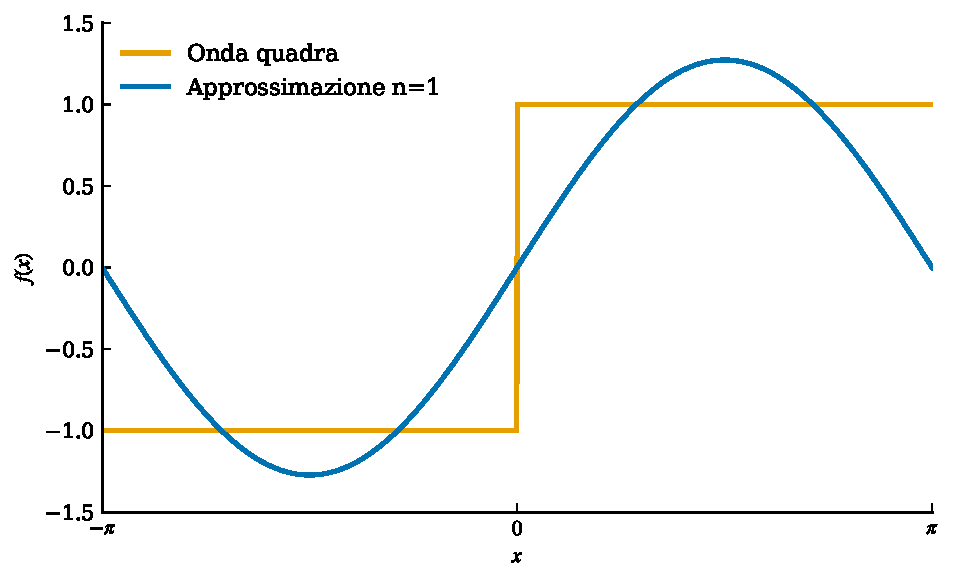
\includegraphics[width=0.5\linewidth]{Fourier_q_1.pdf}\hfill
    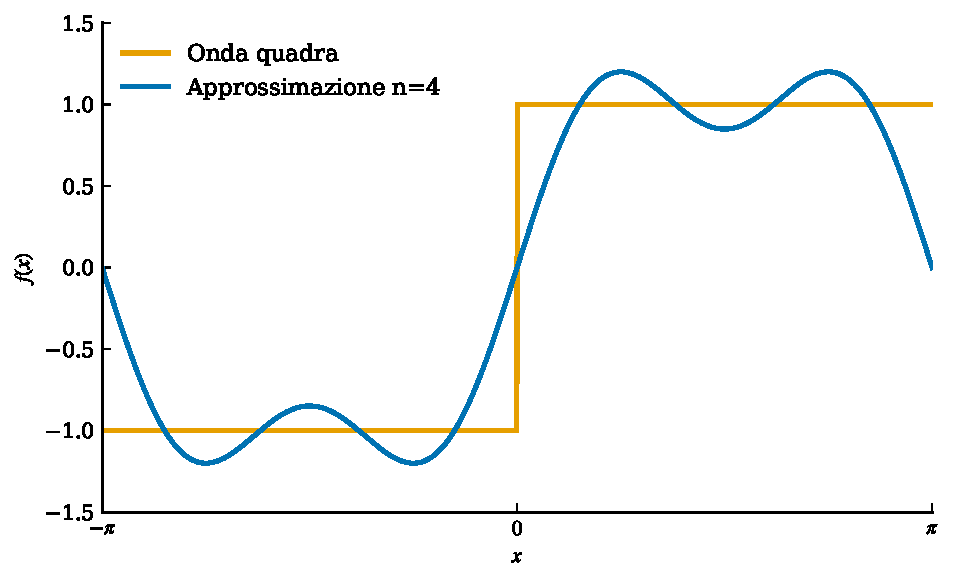
\includegraphics[width=0.5\linewidth]{Fourier_q_4.pdf}\hfill
    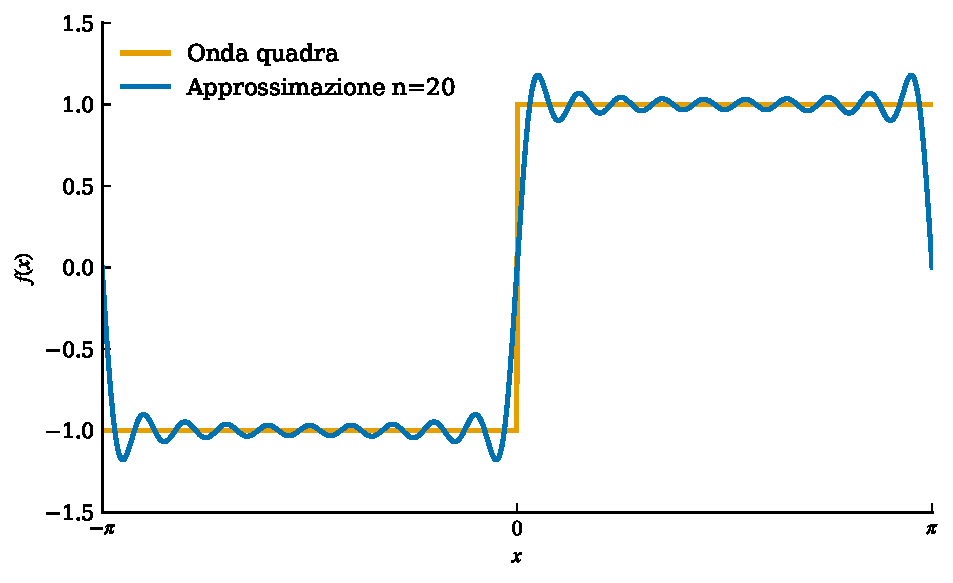
\includegraphics[width=0.5\linewidth]{Fourier_q_20.pdf}\hfill
    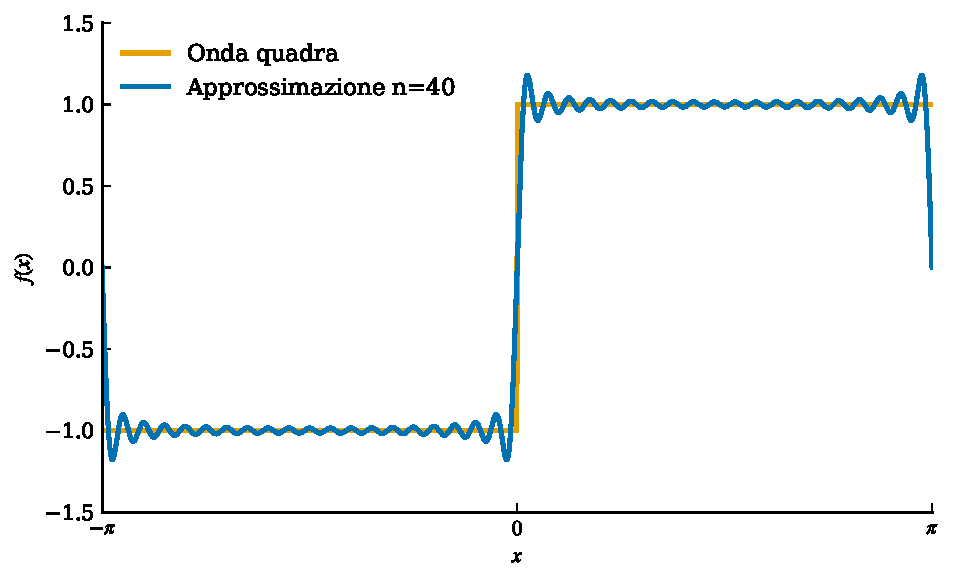
\includegraphics[width=0.5\linewidth]{Fourier_q_40.pdf}
    \end{figure}
    
Un aspetto particolarmente interessante riguarda il comportamento della serie nei punti di discontinuità. In tali punti, la serie di Fourier non converge al valore della funzione (che non è definito in modo continuo), ma al valore medio tra il limite destro e il limite sinistro. Questo fenomeno si manifesta graficamente con delle oscillazioni caratteristiche in prossimità dei salti, note come fenomeno di Gibbs: anche aumentando il numero di termini, queste oscillazioni non scompaiono del tutto, ma si concentrano sempre più vicino al punto di discontinuità, mantenendo però un’ampiezza relativa non trascurabile.
Dal punto di vista delle frequenze, ogni termine della serie aggiunge un’oscillazione con frequenza sempre più alta, contribuendo a ricostruire i dettagli più fini della funzione. Le componenti a bassa frequenza determinano la forma globale del grafico, mentre quelle ad alta frequenza raffinano l’approssimazione nelle zone dove la funzione varia più rapidamente. Questo permette di interpretare la serie di Fourier come una decomposizione della funzione in modi normali, ciascuno associato a una specifica scala di variazione. Infine, è importante osservare che la convergenza della serie non è uniforme in presenza di discontinuità: mentre lontano dai punti critici l’approssimazione migliora rapidamente, nelle loro vicinanze il miglioramento è più lento e presenta le oscillazioni descritte. Questo evidenzia come la serie di Fourier sia uno strumento estremamente potente per analizzare funzioni periodiche, ma richieda anche una corretta interpretazione nei casi non regolari.    
  
       
       
       
 


\newpage

\subsection{Esempio: onda triangolare}

Prendiamo in esame un altro caso classico, ovvero l'onda triangolare $f(x)=d(\pi-|x|)$.

\begin{itemize}
    \item\underline{Forma esponenziale}: Calcoliamoci $c_0=\displaystyle\frac{1}{2\pi}\int_{-\pi}^\pi f(x) \,dx=\frac{d}{\pi}\int_0^\pi(\pi-x)\,dx=\frac{\pi d}{2}$. Poi $c_k=\displaystyle\frac{1}{2\pi}\int_{-\pi}^\pi f(x)e^{-ikx}\,dx=\frac{1}{2\pi}\int_{-\pi}^\pi f(x)(\cos(kx)-i\sin(kx))\,dx$ e dato che $f(x)$ è pari abbiamo che solo l'integrale di $\cos(kx)f(x)\implies c_k=\displaystyle\frac{1}{2\pi}\int_{-\pi}^\pi f(x)\cos(kx)\,dx=\frac{d}{\pi}\int_0^\pi(\pi-x)\cos(kx)\,dx=\frac{d}{\pi}\bigg[\pi\int_0^\pi\cos(kx)\,dx-\int_0^\pi x\cos(kx)\,dx\bigg]=\frac{d}{\pi}\bigg[0-\frac{-1-(-1)^k}{k^2}\bigg]$.
    \\
    \\Quindi $c_k=\displaystyle\frac{d(1-(-1)^k)}{\pi k^2}\implies f(x)=\displaystyle\frac{\pi d}{2}+\sum_{k=-\infty}^\infty\frac{d(1-(-1)^k)}{\pi k^2}e^{ikx}$.
    \item\underline{Forma trigonometrica}: Dal calcolo precedente sappiamo che $b_n=0 \ \ \forall n$, quindi limitiamoci a calcolare $a_0=\displaystyle\frac{1}{\pi}\int_{-\pi}^\pi f(x)\,dx=\frac{2}{\pi}\int_0^\pi d(\pi-x) \,dx=\pi d$. Mentre per i coefficienti $a_n$
    si ha $a_n=\displaystyle\frac{1}{\pi}\int_{-\pi}^\pi f(x) \cos(nx)\,dx=\frac{2d(1-(-1)^n)}{\pi n^2}$, quindi in questo 
    \\
    \\caso abbiamo $f(x)=\displaystyle\frac{\pi d }{2}+\sum_{n=1}^\infty\frac{2d(1-(-1)^n)}{\pi n^2}\cos(nx)=\frac{\pi d}{2}+\frac{4d}{\pi}\sum_{k=0}^\infty\frac{\cos((2k+1)x)}{(2k+1)^2} $.
\end{itemize}

Nel caso dell’onda triangolare, il confronto tra la forma trigonometrica e quella esponenziale segue la stessa logica vista per l’onda quadra, ma con alcune differenze legate alla maggiore regolarità della funzione.
Anche in questo caso la forma trigonometrica permette una lettura più immediata della struttura della serie: la funzione viene ricostruita come somma di oscillazioni cosinusoidali e, per effetto della simmetria, scompaiono completamente i termini sinusoidali. Questo rende evidente che la funzione è costruita a partire da armoniche selezionate e che il contributo delle frequenze elevate diminuisce più rapidamente rispetto al caso dell’onda quadra, riflettendo una maggiore “morbidezza” della funzione.
Nella forma esponenziale, invece, la stessa informazione viene raccolta in un’unica somma di esponenziali, senza separare esplicitamente le diverse componenti trigonometriche. Anche in questo caso, come per l’onda quadra, la struttura della serie mette in evidenza la presenza solo determinate armoniche, mentre le altre vengono annullate dalla simmetria della funzione. Tuttavia, a differenza del caso precedente, qui i coefficienti decrescono più rapidamente (con $n^{-2}$ e $k^{-2}$), e questo è una conseguenza diretta della maggiore regolarità dell’onda triangolare rispetto all’onda quadra.


In entrambi i casi analizzati abbiamo notato che la simmetria della funzione gioca un ruolo centrale nella struttura della serie di Fourier. Non si limita infatti a semplificare i calcoli, ma interviene direttamente nella composizione della serie, determinando quali termini possono effettivamente contribuire alla ricostruzione della funzione. In particolare, la simmetria agisce come un vero e proprio “filtro strutturale”: elimina alcune componenti e seleziona solo le frequenze più compatibili con la struttura della funzione. Di conseguenza, non tutte le armoniche hanno lo stesso ruolo nella ricostruzione, ma solo alcune sopravvivono allo sviluppo. Questo aspetto mette in evidenza che la forma della serie non dipende soltanto dal calcolo dei coefficienti, ma è già fortemente determinata dalle proprietà intrinseche della funzione, in particolare dalle sue simmetrie.

\newpage

\subsubsection{\underline{Interpretazione grafica}}
\vspace{0.5cm}
L’interpretazione grafica della serie di Fourier dell’onda triangolare segue lo stesso schema visto per l’onda quadra: aumentando il numero di termini della somma, l’approssimazione della funzione migliora progressivamente. Tuttavia, in questo caso la convergenza è sensibilmente più rapida; infatti già con pochi termini la forma generale della funzione è ben riconoscibile, e l’aggiunta di armoniche successive serve soprattutto a rifinire i dettagli della ricostruzione. A differenza dell’onda quadra, non compaiono oscillazioni evidenti nelle zone critiche e l’approssimazione risulta più stabile già a bassi ordini. 

    \begin{figure}[H]
    \centering
    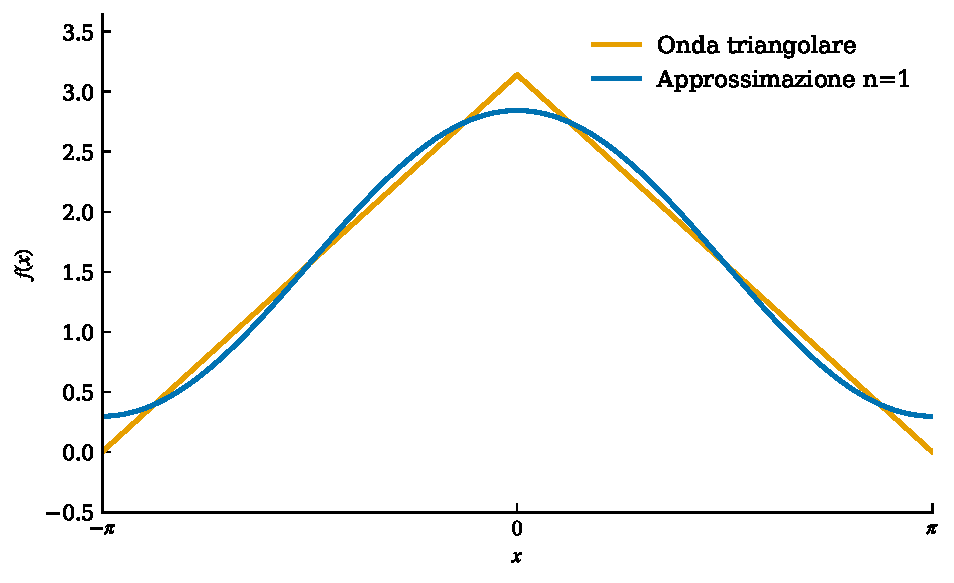
\includegraphics[width=0.5\linewidth]{Fourier_t_1.pdf}\hfill
    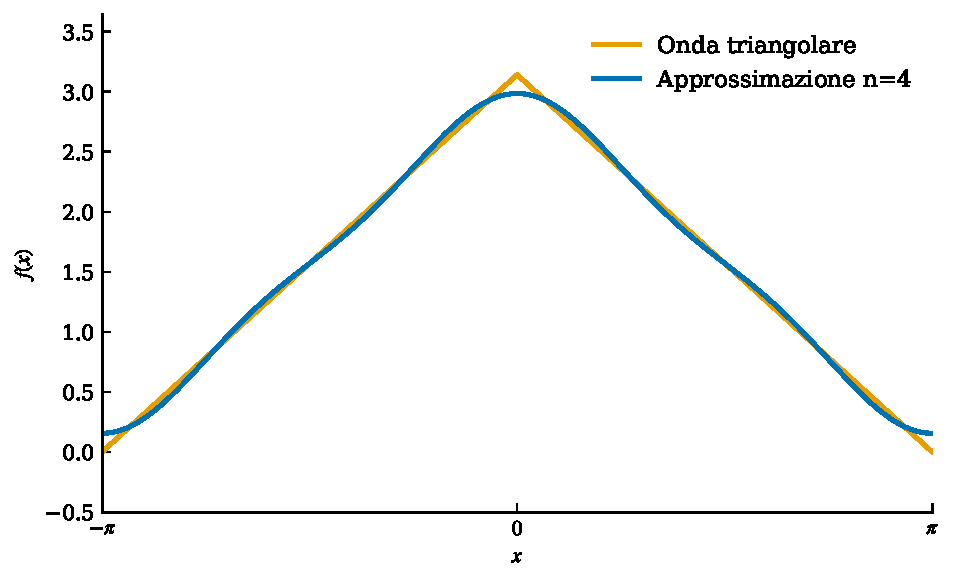
\includegraphics[width=0.5\linewidth]{Fourier_t_4.pdf}\hfill
    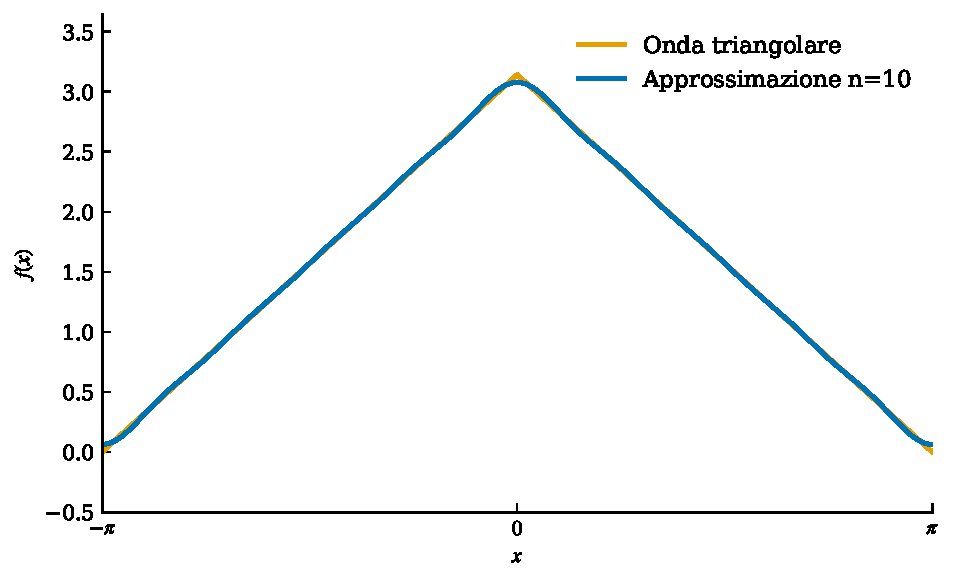
\includegraphics[width=0.5\linewidth]{Fourier_t_10.pdf}\hfill
    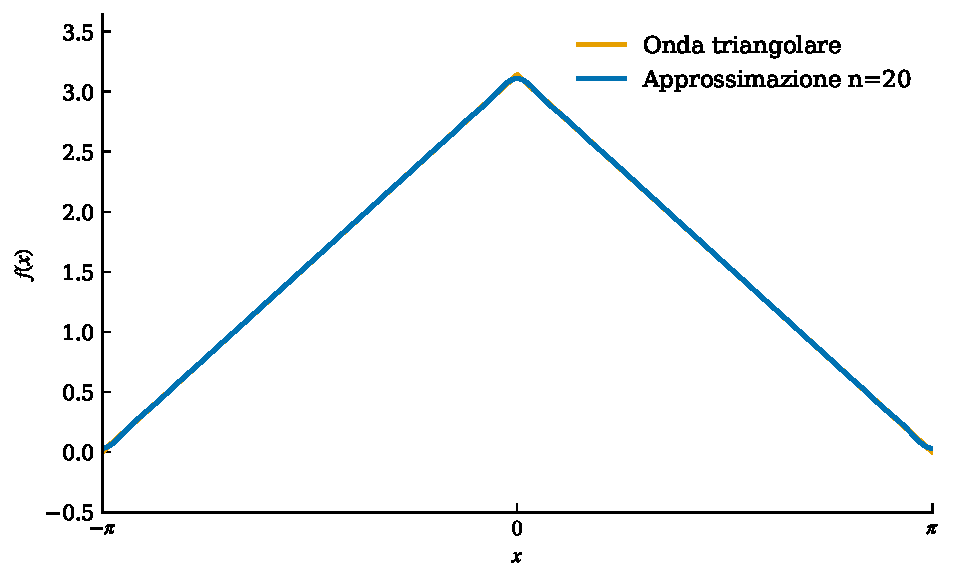
\includegraphics[width=0.5\linewidth]{Fourier_t_20.pdf}
    \end{figure} 

Questo comportamento è legato alla maggiore regolarità dell’onda triangolare: la funzione è continua su tutto l’intervallo e presenta solo punti angolosi nei vertici. Questa maggiore “morbidezza” si riflette direttamente nella velocità di convergenza della serie di Fourier, i cui coefficienti decrescono più rapidamente rispetto al caso dell’onda quadra, come abbiamo visto. Di conseguenza, i termini con indice elevato contribuiscono sempre meno alla somma, e già pochi addendi sono sufficienti per ottenere una buona approssimazione. Un altro aspetto rilevante è che l’approssimazione mantiene una forma molto stabile anche vicino ai punti di non derivabilità: non compaiono oscillazioni marcate e la funzione ricostruita segue fedelmente l’andamento lineare a tratti dell’onda triangolare. Questo rende la serie particolarmente efficace nel descrivere funzioni continue ma non perfettamente lisce. Infine, si può osservare che ogni termine della serie introduce una correzione sempre più fine, ma senza alterare in modo significativo la struttura globale del grafico. In questo senso, la costruzione della funzione tramite somme parziali risulta più regolare e prevedibile rispetto al caso dell’onda quadra, offrendo un esempio chiaro di come la regolarità della funzione influenzi direttamente la qualità e la rapidità della sua approssimazione tramite serie di Fourier

\newpage
    
\subsection{Esempio avanzato: funzione complessa}    
        
Analizziamo adesso un esempio più articolato, questo paragrafo non essenziale per la comprensione degli argomenti che seguiranno. Consideriamo una funzione a valori complessi $f(x):[-\pi,\pi]\to \mathbb{C}$ definita come $f(x)=\displaystyle\frac{1}{i\pi}\ln \bigg(\frac{1+e^{ix}}{1-e^{ix}}\bigg)$. 

\begin{itemize}
    \item\underline{Forma esponenziale}: Come prima cosa calcoliamo i coefficienti $c_k$ della serie di Fourier esponenziale con $k\neq 0$.
    \\
    \\ Quindi $c_k=\displaystyle\frac{1}{2 i\pi^2}\int_{-\pi}^\pi\ln\bigg(\frac{1+e^{ix}}{1-e^{ix}}\bigg)e^{-ikx}\,dx=\frac{1}{2i\pi^2}\int_{-\pi}^\pi\bigg[\ln(1+e^{ix})-\ln(1-e^{ix})\bigg]e^{-ikx}\,dx$
    \\
    \\
    \\Sviluppando i logaritmi in serie con $e^{ix}=z$ (dimostrazione  (\ref{app. 19})), otteniamo:
    \\
    \\ $c_k=\displaystyle\frac{1}{2i\pi^2}\int_{-\pi}^\pi\sum_{n=1}^\infty\bigg[\frac{(-1)^{n-1}}{n}z^n+\frac{z^n}{n}\bigg]e^{-ikx}\,dx=\frac{1}{2i\pi^2}\int_{-\pi}^\pi\sum_{n=1}^\infty\frac{1-(-1)^n}{n}e^{inx}e^{-ikx}\,dx$
    \\
    \\
    \\$=\displaystyle\frac{1}{2i\pi^2}\sum_{n=1}^\infty\frac{1-(-1)^n}{n}\int_{-\pi}^\pi e^{i(n-k)x}\,dx=\frac{1}{2i\pi^2}\sum_{n=1}^\infty\frac{1-(-1)^n}{n}2\pi \delta_{nk}$, ponendo $n=k$ 
    \\
    \\
    \\otteniamo quindi $c_k=\displaystyle\frac{1}{2i\pi^2}\frac{1-(-1)^k}{k}2\pi=\frac{1-(-1)^k}{i\pi k}\implies c_k=\frac{1-(-1)^k}{i\pi k}$.
    \\
    \\ Quindi la nostra funzione assume la forma $f(x)=c_0+\displaystyle\sum_{k=-\infty}^\infty\frac{1-(-1)^k}{i\pi k}e^{ikx}$. 
    \\Dobbiamo ancora determinare il valore di $c_0$. In questo caso particolare notiamo che l'espansione che abbiamo utilizzato della funzione è $f(x)=\displaystyle\sum_{n=1}^\infty\frac{1-(-1)^n}{i\pi n}e^{inx}$. 
    \\Questo è molto interessante perchè notiamo che la funzione è naturalmente decomposta in una base di esponenziali complessi, tuttavia potrebbe trattarsi di una base non normalizzata. Il fatto però che i coefficienti delle somme coincidano perfettamente ci suggerisce che l'espansione utilizzata (in questo caso ribadiamo) è a tutti gli effetti una decomposizione su una base ortonormale di esponenziali complessi, da cui deduciamo $c_0=0, \ k\in[1,\infty).$
    \\
    \\ Quindi $f(x)=\displaystyle\sum_{k=1}^\infty\frac{1-(-1)^k}{i\pi k}e^{ikx}=\frac{2}{i\pi }\sum_{h=0}^\infty \frac{e^{i(2h+1)x}}{2h+1}$.
    \\
    \\ Notiamo ora una cosa molto interessante: l'espressione della serie di Fourier appena calcolata è molto simile a quella dell'onda quadra (\ref{sec: 3.4.3}).
    \\ 
    \\Notiamo infatti che $\Re(f)=\frac{1}{2}(f+f^*)=\displaystyle\frac{1}{2}\bigg(\sum_{k=1}^\infty\frac{1-(-1)^k}{i\pi k}e^{ikx}-\sum_{k=1}^\infty\frac{1-(-1)^k}{i\pi k}e^{-ikx}\bigg) $ 
    \\$=\frac{1}{2}\sum_{k=\infty}^\infty\frac{1-(-1)^k}{i\pi k}e^{ikx}\implies\Re(f)=\frac{1}{2}\sum_{k=\infty}^\infty\frac{1-(-1)^k}{i\pi k}e^{ikx}$ che coincide con l'espressione della serie di Fourier dell'onda quadra riscalata di un fattore $\frac{1}{2}$.
\end{itemize}

\newpage

\subsubsection{\underline{Interpretazione grafica}}

\vspace{0.5cm}

Qui l’interpretazione grafica è decisamente più interessante rispetto ai casi precedenti, perché la funzione non viene soltanto vista come una combinazione di oscillazioni reali, ma emerge in modo naturale come somma di contributi che, nel piano complesso, hanno un’interpretazione geometrica immediata. Ogni termine $e^{ikx}$ può infatti essere interpretato come una rotazione a velocità costante, in cui il modulo rimane invariato mentre la fase varia linearmente con $x$, dando origine a un moto regolare di tipo elicoidale. Inoltre, in questo caso, la funzione può essere visualizzata sia come evoluzione nello spazio complesso delle sue componenti oscillanti, sia attraverso la sua proiezione sul piano reale (che abbiamo visto essere un'onda quadra).

\begin{figure}[H]
    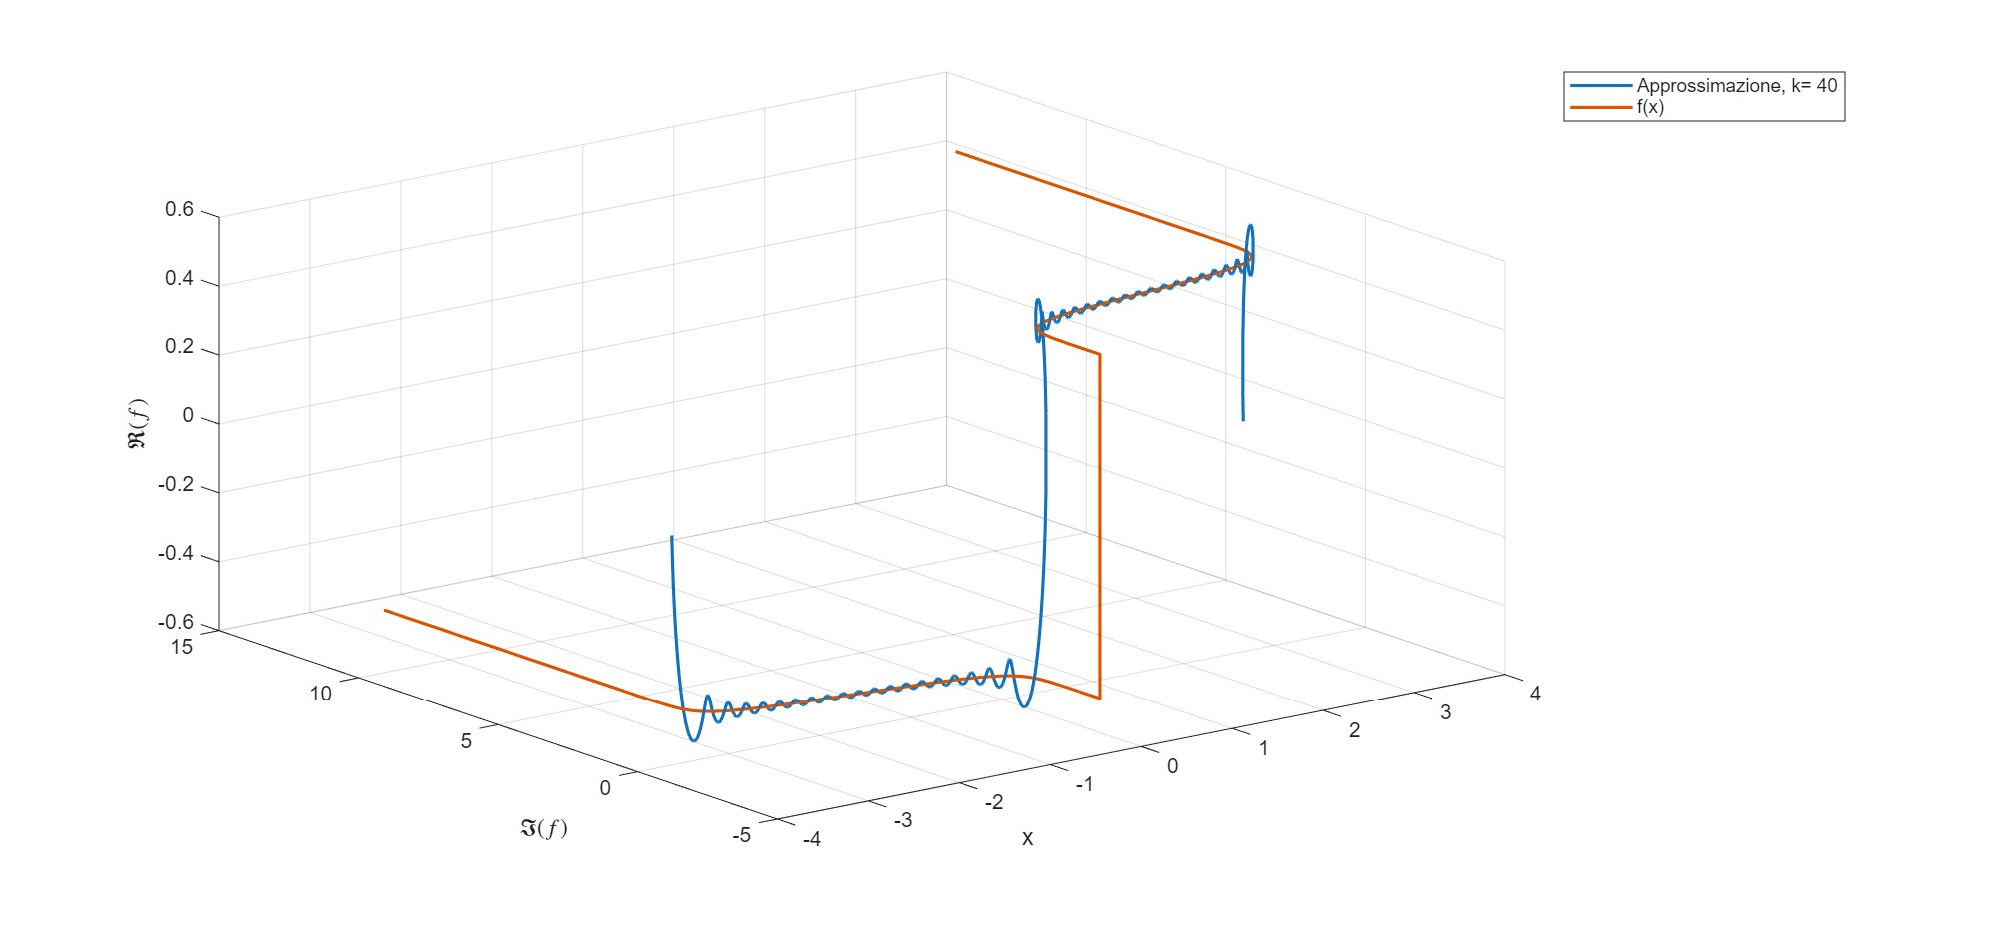
\includegraphics[width=0.6\linewidth]{logaritmo_strano_IMPARAAFAREICALCOLI.pdf}\hfill
    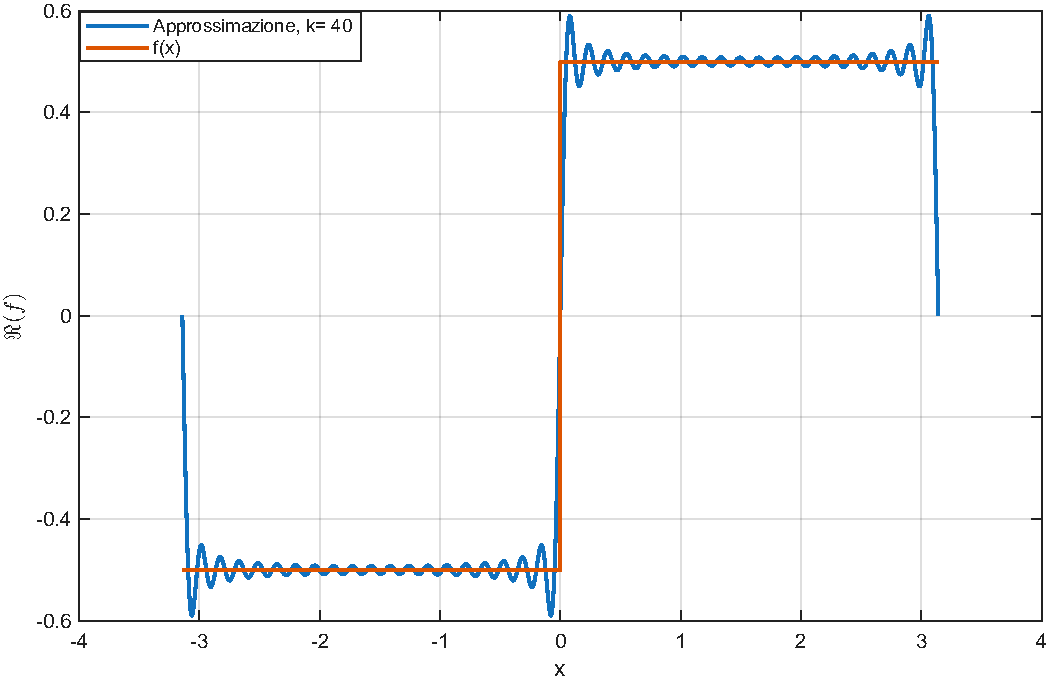
\includegraphics[width=0.4\linewidth]{con_griglia.pdf}
\end{figure}

Le immagini associate mettono in evidenza proprio questo doppio livello di lettura. Da un lato, la rappresentazione nello spazio complesso mostra la costruzione della funzione come somma di contributi rotanti, ciascuno associato a una diversa frequenza (in questa visione la funzione non è più un semplice andamento su un asse, ma una struttura dinamica che si sviluppa attraverso la sovrapposizione di moti elementari), dall’altro lato, la proiezione sul piano reale restituisce un risultato sorprendentemente semplice: l’onda quadra riscalata di un fattore 1/2. Questo passaggio è particolarmente significativo perché mostra come una struttura apparentemente più astratta e complessa possa generare, attraverso una semplice operazione di estrazione della parte reale, una funzione reale ben nota e immediatamente interpretabile.

Questo esempio evidenzia in modo particolarmente chiaro la potenza della rappresentazione in serie di Fourier nel dominio complesso. A differenza dei casi precedenti, qui la funzione non viene soltanto approssimata o scomposta, ma costruita direttamente come combinazione di esponenziali complessi che contengono l’intera informazione analitica.
Un aspetto notevole è che la struttura complessa “intermedia” non è un artificio tecnico, ma una vera e propria estensione geometrica della funzione, nella quale le informazioni sono distribuite su una dimensione più ricca. La funzione reale emerge quindi non come oggetto indipendente, ma come proiezione di una struttura più generale.
Infine, il confronto tra la rappresentazione complessa e la sua proiezione reale mette in evidenza come le serie di Fourier non siano soltanto uno strumento di decomposizione, ma anche un mezzo per visualizzare funzioni come somma di contributi oscillatori elementari, la cui interazione produce forme estremamente semplici e riconoscibili nello spazio reale.

\newpage

\section{Convergenza delle serie di Fourier}

Dopo aver studiato la costruzione delle serie di Fourier e le loro principali proprietà, in questa sezione affronteremo in modo più approfondito il problema della convergenza. In particolare, ci porremo una domanda fondamentale: in che senso la serie di Fourier di una funzione rappresenta effettivamente la funzione stessa?
\\Sappiamo che, in un opportuno contesto, la convergenza è garantita in norma $L^2$ (cioè in media sull’intervallo), ma questo non garantisce la convergenza locale. Per questo motivo analizzeremo condizioni che assicurano la convergenza puntuale, introducendo strumenti come il nucleo di Dirichlet e il lemma di Riemann–Lebesgue, e discuteremo il ruolo della condizione di Dini. Studieremo inoltre il comportamento della serie nei punti di discontinuità, dove emergerà il fenomeno della convergenza alla media dei limiti destro e sinistro, mettendo in evidenza come la serie di Fourier interpreti localmente la funzione. Infine, esamineremo il legame tra la regolarità della funzione e la decrescita dei coefficienti di Fourier, mostrando come proprietà qualitative della funzione si riflettano direttamente nel comportamento della sua serie. In questo modo, la teoria delle serie di Fourier si inserisce naturalmente nel quadro più generale degli spazi funzionali, evidenziando la relazione tra convergenza, regolarità e struttura dello spazio in cui si lavora.

\subsection{Nucleo di Dirichlet}

Per studiare la convergenza puntuale delle serie di Fourier, è utile riscrivere le somme parziali in una forma che ne chiarisca meglio il comportamento locale. L’idea è che la serie non vada vista solo come somma di esponenziali complessi, ma come una combinazione dei valori della funzione vicini al punto in cui la si valuta. In questo modo si può interpretare la somma parziale come una sorta di media pesata della funzione attorno a quel punto, e in questo contesto emerge naturalmente il nucleo di Dirichlet.

\begin{definizione}[Nucleo di Dirichlet]
    Definiamo nucleo di Dirichlet la funzione 
    \\$D_n: \mathbb{R}\to\mathbb{R}$ della forma $D_n(t)=:\displaystyle\frac{1}{2\pi}\sum_{k=-n}^n e^{ikt}$.
\end{definizione}

\underline{\textbf{Nota}}: Apparentemente $D_n(t)$ potrebbe sembrare una funzione a valori complessi data la presenza dell'esponenziale tuttavia; data la simmetria della somma parziale, per ogni $\tilde{k}$ si ha $e^{i\tilde{k}t}+e^{-i\tilde{k}t}=\cos(\tilde{k}t)+i\sin{(\tilde{k}t})+\cos(\tilde{k}t)-i\sin({\tilde{k}t})=2\cos(\tilde{kt)}$. Quindi, le parti immaginarie si elidono vicendevolmente, lasciandoci un "output" reale.

\begin{proposizione}
    Il nucleo di Dirichlet si può esprimere nella seguente forma equivalente: $D_n(t)=\displaystyle\frac{\sin((n+1\backslash2)t)}{2\pi\sin( t\backslash2)}$.
    \\
    \\ \underline{Dimostrazione}: Notiamo che $\displaystyle\sum_{k=-n}^ne^{ikt}=\sum_{j=0}^{2n}e^{i(j-n)t}=e^{-int}\sum_{j=0}^{2n}(e^{it})^j=e^{-int}\frac{1-(e^{it})^{2n+1}}{1-e^{it}}$, dopodichè riscriviamo il denominatore: $-(e^{it}-1)=-(e^{it\backslash2}(e^{it\backslash2}-e^{-it\backslash2}))=-(e^{it\backslash2}(2i\sin(t\backslash2))$.
    \\ 
    \\E similmente il nominatore: $e^{int}(1-e^{i(2n+1)t})=e^{int}(-2ie^{i(2n+1)t\backslash2}\sin((n+1\backslash2)t))$.
    \\
    \\ Quindi, ricomponendo, si ha $\displaystyle\sum_{k=-n}^ne^{ikt}=\frac{\sin((n+1\backslash2)t)}{\sin( t\backslash2)}\implies D_n(t)=\frac{\sin((n+1\backslash2)t)}{2\pi\sin( t\backslash2)}$. \qed
\end{proposizione}

\newpage

Cerchiamo adesso di analizzare la struttura di questo nucleo di Dirichlet appena definito e di evincerne alcune proprietà che si riveleranno essere determinanti:

\begin{itemize}
    \item \underline{Normalizzazione}: Se calcoliamo l'integrale del $D_n$ notiamo che questo è perfettamente normalizzato, infatti: $\displaystyle\int_{-\pi}^\pi D_n(t)\,dt=\frac{1}{2\pi}\int_{-\pi}^\pi \sum_{k=-n}^n e^{ikt} \,dt=\frac{1}{2\pi}\sum_{k=-n}^n\int_{-\pi}^\pi e^{ikt}\,dt$
    \\ $=\displaystyle\frac{1}{2\pi}\bigg(\int_{-\pi}^\pi1 \,dt+\sum_{k\neq 0}\int_{-\pi}^\pi e^{ikt}\,dt\bigg)=\frac{1}{2\pi}\bigg(2\pi+0\bigg)=1$.
    \\
    \item\underline{Non positività e natura oscillatoria}: Si nota facilmente che $D_n(t)$ non è definito positivo, infatti basta fare alcuni conti. Prendiamo ad esempio $t=\frac{2\pi}{3}\implies \sin(t\backslash2)=\sin(\pi\backslash3)\gt 0$, tuttavia il nominatore oscillerà tra valori positivi e negativi al variare del parametro $n$, da cui deduciamo che esistono infiniti $n$ per cui $D_n(t)\gt 0$ e $D_n(t)\lt 0$. Notiamo inoltre che le oscillazioni del nominatore crescono in maniera direttamente proporzionale all'aumentare di $n$; infatti il numero di zeri sull'intervallo $[-\pi,\pi]$ sarà circa $2n$.
\end{itemize}

Prendiamo adesso una generica funzione $f\in L^2([-\pi, \pi])$ con la sua relativa serie di Fourier esponenziale (\ref{def: 3.26}), notiamo che possiamo definire le somme parziali di quest'ultima tramite il nucleo di Dirichlet:
\\
\\ $f_n(x)=\displaystyle\sum_{k=-n}^nc_ke^{ikx}=\frac{1}{2\pi}\sum_{k=-n}^n\bigg(\int_{-\pi}^\pi f(y)e^{-iky}\,dy\bigg)e^{ikx}=\frac{1}{2\pi}\sum_{k=-n}^n\int_{-\pi}^\pi f(y)e^{i(x-y)k} \,dy=$
\\$\displaystyle\int_{-\pi}^\pi f(y)\frac{1}{2\pi}\sum_{k=-n}^ne^{i(x-y)k}\,dy=\int_{-\pi}^\pi f(y) D_n(x-y) \,dy \implies f_n(x)=\int_{-\pi}^\pi f(y) D_n(x-y)\,dy$
\\
\\
\\Abbiamo dimostrato di poter riscrivere le somme parziali della serie di Fourier di una funzione $f(x)$ come la convoluzione (\ref{def: 3.23}) tra la funzione stessa e il nucleo di Dirichlet. 
\\ Le somme parziali della serie di Fourier possono essere quindi interpretate come un operatore che associa alla funzione originale una nuova funzione ottenuta combinando i valori della funzione stessa in un intorno di ciascun punto. In questo processo emerge in modo naturale il nucleo di Dirichlet, che agisce come insieme di pesi con cui vengono mediati i valori della funzione attorno al punto considerato. Notiamo che la proprietà di normalizzazione del nucleo fa si che l’operazione non modifichi il "livello medio della funzione" a livello globale e che, almeno formalmente, si comporti come una sorta di media pesata dei valori della funzione. Tuttavia, questa interpretazione ha dei limiti importanti: il nucleo di Dirichlet non è positivo, e quindi non può essere interpretato come una vera media nel senso classico, cioè come combinazione convessa di valori (ovvero una combinazione lineare di valori della stessa funzione a coefficienti non negativi). La presenza di valori positivi e negativi implica che nella somma si verifichino cancellazioni che possono essere anche molto significative.
A questo si aggiunge un ulteriore aspetto cruciale: il nucleo è fortemente oscillatorio e le sue oscillazioni diventano sempre più rapide al crescere dell’indice (come abbiamo notato sopra). Questo implica che il contributo dei valori della funzione non si distribuisce in modo regolare, ma alterna continuamente segni, generando un comportamento altamente instabile dal punto di vista dell’approssimazione. Nel complesso, queste tre proprietà mostrano che, pur avendo una struttura che ricorda quella di un operatore di media grazie alla normalizzazione, il nucleo di Dirichlet non può essere considerato un vero kernel di approssimazione. La mancanza di positività e la forte natura oscillatoria del nucleo di Dirichlet impediscono un vero comportamento regolarizzante, a differenza di quanto accade nei kernel di approssimazione positivi introdotti nei teoremi di Weierstrass (\ref{thm: 3.11}) e Fejer (\ref{thm: 3.12}). In quei casi, la positività dei pesi garantisce che l’operazione agisca come una media locale stabile, che “smussa” la funzione e assicura una convergenza ben controllata.
Nel caso di Dirichlet, invece, la presenza di termini di segno alterno introduce cancellazioni tra contributi vicini, rendendo l’effetto complessivo molto più delicato e non monotono. Di conseguenza, lo studio della convergenza non può più basarsi su argomenti di tipo regolarizzante, ma richiede strumenti più raffinati in grado di controllare direttamente le oscillazioni del nucleo e il comportamento locale della funzione. Nel paragrafo successivo introdurremo proprio questi strumenti, a partire da un risultato fondamentale sull’attenuazione delle oscillazioni ad alta frequenza: il lemma di Riemann-Lebesgue.

\subsection{Convergenza puntuale}

Dopo aver reinterpretato le somme parziali della serie di Fourier come convoluzioni con il nucleo di Dirichlet, il problema della convergenza puntuale si riduce allo studio del comportamento di un integrale in cui intervengono pesi fortemente oscillanti (dati per l'appunto da $D_n(t)$). Quindi adesso, la questione centrale diventa comprendere in che senso tali oscillazioni incidano o meno sul valore limite della successione $f_n(x)$. La mancanza di positività del nucleo di Dirichlet esclude la possibilità di interpretare la convoluzione come una media locale di tipo regolarizzante, come invece accade per i kernel positivi introdotti nei teoremi di Weierstrass e Fejer. Di conseguenza, la convergenza non può essere dedotta da proprietà di monotonia o di stabilità della media. In questo paragrafo verranno quindi introdotti gli strumenti fondamentali per affrontare questo problema: il lemma di Riemann–Lebesgue, che descrive l’effetto delle oscillazioni ad alta frequenza, e la condizione di Dini, che fornisce un criterio locale sulla funzione sufficiente a garantire la convergenza puntuale della serie di Fourier. Questi risultati porteranno infine al teorema di convergenza puntuale e alla sua interpretazione nei casi in cui la funzione sia continua o sufficientemente regolare nel punto, e nei casi in cui presenti discontinuità di salto.

\begin{lemma}[Lemma di Riemann-Lebesgue]
    Sia $f(x)\in L^1([-\pi,\pi])$. Allora vale il seguente limite: $\displaystyle\lim_{|k|\to\infty}\int_{-\pi}^\pi f(x) e^{ikx}\,dx=0$.
    \\
    \\ \underline{Dimostrazione}: Sia $P(x)=\displaystyle\sum_{n=-N}^Na_ne^{inx}$ un polinomio trigonometrico (\ref{def: 3.24}) e notiamo che vale $\displaystyle\int_{-\pi}^\pi P(x) e^{ikx} \,dx=\sum_{n=-N}^Na_n\int_{-\pi}^\pi e^{i(n+k)x}\,dx=\sum_{n=-N}^Na_n2\pi \delta_{nk}$. Deduciamo quindi che $\displaystyle\int_{-\pi}^\pi P(x)e^{ikx}\,dx=0$ se $|k|\gt N$ (perchè avremmo necessariamente $\delta_{nk}=0$).
    \\ Per il teorema di Fejer (\ref{thm: 3.12}) sappiamo che $\exists P$ tale che $\|f-P\|_1\lt \varepsilon$. 
    \\
    \\Tenendo a mente ciò scriviamo $\displaystyle\int_{\pi}^\pi f(x)e^{ikx}\,dx=\int_{-\pi}^\pi (f-P)e^{ikx}\,dx+\int_{-\pi}^\pi P e^{ikx}\,dx$.
    \newpage

     Analizzando il primo termine deduciamo $\bigg|\displaystyle\int_{-\pi}^\pi(f-P)e^{ikx}\,dx\bigg|\leq \int_{-\pi}^\pi |f-P|e^{ikx}\,dx=\varepsilon $.
     \\ Per quanto riguarda il secondo, se estrinsechiamo $P=\displaystyle\sum_{n=-N}^Na_ne^{inx}$, notiamo che, per quanto detto prima, l'integrale $\displaystyle\int_{-\pi}^\pi  Pe^{ikx}\,dx$ è nullo se $|k|\gt N$. Quindi per $|k|\gt N$ abbiamo $\bigg|\displaystyle\int_{-\pi}^\pi f(x)e^{ikx}\,dx\bigg|\lt \varepsilon\implies \lim_{|k|\to\infty}\int_{-\pi}^\pi f(x)e^{ikx}\,dx=0$. \qed
\end{lemma}

Prima di utilizzare il lemma di Riemann–Lebesgue nel contesto delle serie di Fourier, è necessario introdurre una condizione locale sulla funzione che consenta di controllare in modo adeguato il termine che compare nella rappresentazione delle sue somme parziali tramite il nucleo di Dirichlet. Non è infatti sufficiente assumere la sola integrabilità globale di $f(x)$ (quindi assumere $f\in L^1([-\pi,\pi])$), poiché nella formula delle somme parziali il comportamento rilevante è quello della funzione in un intorno arbitrariamente piccolo del punto considerato. Ciò è dovuto alla presenza del nucleo di Dirichlet; esso, infatti, può essere interpretato in modo euristico come una successione di nuclei che, pur non essendo positivi, tendono a “concentrare” il proprio effetto sempre più vicino a $t=0$. Questo accade perché, mentre la sua massa totale resta costante e uguale a 1, le oscillazioni del numeratore diventano sempre più rapide al crescere di $n$, producendo cancellazioni sempre più efficaci lontano dall’origine (cioè un progressivo annullamento reciproco dei contributi positivi e negativi dovuto all’alternanza sempre più fitta dei segni nella funzione integranda). In particolare, fuori da ogni intorno fissato di 0, i contributi positivi e negativi si compensano sempre meglio, rendendo trascurabile il contributo complessivo in quelle regioni. Di conseguenza, nella convoluzione rimane rilevante solo il comportamento della funzione in un intorno sempre più piccolo di $t=0$, e il nucleo si comporta quindi come se “concentrasse” la propria azione attorno all’origine, analogamente a quanto avviene per la delta di Dirac (\ref{app: .31}), nel senso che, nelle convoluzioni, il suo effetto finisce per dipendere sempre più soltanto dal valore della funzione nel punto considerato.
In questo senso, il problema non è più di natura globale, ma essenzialmente locale: ciò che influisce sulla convergenza è il modo in cui la funzione si comporta su scale sempre più piccole attorno al punto fisso $x$ (quindi per $t\to 0$). Per poter sfruttare in modo efficace il principio di cancellazione delle alte frequenze fornito dal lemma di Riemann–Lebesgue, è quindi necessario disporre di una condizione di regolarità locale che garantisca un controllo adeguato degli incrementi della funzione.
A questo scopo si introduce la cosiddetta condizione di Dini, che fornisce precisamente tale controllo e che risulta sufficiente a garantire la convergenza puntuale delle somme parziali della serie di Fourier.

\begin{definizione}[Condizione di Dini]
    Sia $f(x)\in L^1([-\pi,\pi])$ e sia $x\in (-\pi,\pi)$. Diremo che $f$ rispetta la condizione di Dini nel punto $x$ se esiste $\delta\gt 0$ tale che:
    \\
    \\$\displaystyle\frac{f(x-t)-f(x)}{t}\in L^1([-\pi,\pi])\iff\int_{-\pi}^\pi\bigg|\frac{f(x-t)-f(x)}{t}\bigg|\,dx\lt\infty$.
\end{definizione}

La condizione di Dini non è particolarmente restrittiva: richiede solo un controllo locale del comportamento della funzione in un intorno del punto $x$, ed è soddisfatta da molte classi di funzioni regolari. In particolare vale se $f(x)$ è derivabile in $x$, oppure se ammette derivate destra e sinistra finite, poiché in entrambi i casi il rapporto incrementale resta controllato vicino a $0$. È inoltre verificata per funzioni Lipschitziane in un intorno di $x$, dove gli incrementi sono dominati linearmente da $|t|$, e più in generale per funzioni con singolarità deboli o crescita locale moderata. La condizione esclude invece funzioni con oscillazioni troppo violente o singolarità forti tali da rendere non integrabile il rapporto incrementale vicino a $0$. Tuttavia queste situazioni sono proprio quelle in cui non ci si può aspettare una buona convergenza puntuale della serie di Fourier. In questo senso, la condizione di Dini elimina solo comportamenti patologici locali, mantenendosi abbastanza generale da includere praticamente tutte le funzioni regolari di nostro interesse.

\begin{teorema}[Teorema di Dirichlet-Dini o di convergenza puntuale] 
Sia $f(x)\in L^1([-\pi,\pi])$ e sia $x\in (-\pi,\pi)$ un punto in cui valga la condizione di Dini per $f(x)$. Allora le somme parziali della serie di Fourier di $f$ soddisfano il criterio di convergenza puntuale in $x$, ossia $\displaystyle\lim_{n\to\infty} f_n(x)=f(x)$.
\\
\\ \underline{Dimostrazione}: Consideriamo la formulazione delle somme parziali della serie di Fourier di $f(x)$ mediante nucleo di Dirichlet $f_n(x)=\displaystyle\int_{-\pi}^\pi f(x-t)D_n(t)\,dt$, dunque scriviamo:
\\$f_n(x)-f(x)=\displaystyle\int_{-\pi}^\pi f(x-t)D_n(t)\,dt-f(x)\int_{-\pi}^\pi D_n(t)\,dt=\int_{-\pi}^\pi (f(x-t)-f(x))D_n(t)\,dt$
\\Espandendo $D_n(t)$ si ha $f_n(x)-f(x)=\displaystyle\frac{1}{2\pi}\int_{-\pi}^\pi \frac{f(x-t)-f(x)}{t}.\frac{t}{\sin(t\backslash 2)}.\sin\bigg(\bigg(n+\frac{1}{2}\bigg)t\bigg)\,dt$.
\\ 
\\
\\Consideriamo ora $g(x)=\displaystyle\frac{f(x-t)-f(x)}{t}.\frac{t}{\sin(t\backslash2)}$. Quindi $g(x)$ è il prodotto di due funzioni: la prima è in $L^1([-\pi,\pi])$ per ipotesi (condizione del Dini), la seconda è limitata (infatti il suo limite per $t\to0$ è uguale a 2), ne segue che il loro prodotto è anch'esso in $L^1([-\pi,\pi])$. Quindi abbiamo:
\\
\\$f_n(x)-f(x)=\displaystyle\frac{1}{2\pi}\int _{-\pi}^\pi g(x) \sin\bigg(\bigg(n+\frac{1}{2}\bigg)t\bigg)\,dt=$, riscrivendo il termine sinusoidale in forma complessa otteniamo $f_n(x)-f(x)=\frac{1}{4\pi i}\bigg[\int_{-\pi}^{\pi} g(t)\,e^{i\left(n+\frac12\right)t}\,dt +\int_{-\pi}^{\pi} g(t)\,e^{-i\left(n+\frac12\right)t}\,dt
\bigg]$.
\\ 
\\
\\Quindi, per di Riemann-Lebesgue, si ha $\displaystyle\lim_{n\to\infty}(f_n-f)=0\implies \lim_{n\to\infty}f_n(x)=f(x)$. \qed
    
\end{teorema}

Un aspetto fondamentale che emerge dallo studio svolto è la differenza tra convergenza in norma e convergenza puntuale delle serie di Fourier. La convergenza in norma (ad esempio in $L^2([-\pi,\pi])$) descrive un controllo globale medio dell’errore tra funzione e somme parziali, il che significa che la differenza tra funzione e approssimazioni diventa trascurabile in media su tutto il dominio. Tuttavia, questo tipo di convergenza non fornisce informazioni sul comportamento in un singolo punto. La convergenza puntuale, invece, è un fenomeno localmente dipendente, che riguarda il limite di $f(x)$ per ogni singolo $x$. Come abbiamo visto, essa non segue automaticamente dalla convergenza in norma e richiede ipotesi aggiuntive sul comportamento locale della funzione, come la condizione di Dini o, in generale, condizioni di regolarità puntuale. In altre parole, mentre la convergenza in norma garantisce una buona approssimazione globale, la convergenza puntuale descrive in modo molto più fine come la serie si comporta punto per punto, rivelando fenomeni più delicati legati alla struttura locale della funzione e al ruolo oscillatorio del nucleo di Dirichlet.

\newpage

\subsection{Derivabilità e fenomeno di Gibbs}

Come abbiamo visto nel paragrafo precedente, lo studio delle serie di Fourier evidenzia una distinzione fondamentale tra convergenza in norma e convergenza puntuale. La prima descrive un controllo globale dell’errore, mentre la seconda riguarda il comportamento del limite delle somme parziali punto per punto. Questa differenza mostra che la sola convergenza in norma non è sufficiente a descrivere la struttura delle approssimazioni, rendendo necessario introdurre strumenti più raffinati per l’analisi locale. In questa direzione abbiamo osservato come risultati come il teorema di Dirichlet o la condizione di Dini permettano di comprendere in modo preciso il comportamento puntuale delle serie di Fourier. Una volta chiarito questo aspetto, l’attenzione si sposta su un problema complementare: non si tratta più di studiare se la serie converge a una funzione assegnata, ma di analizzare il tipo di funzione che si ottiene come somma della serie di Fourier e quali proprietà di regolarità essa possiede. In questa prospettiva si affrontano ora le questioni legate alla derivabilità delle serie di Fourier e al fenomeno di Gibbs.

La prima domanda che ci poniamo riguarda la regolarità della funzione ricostruita: in particolare ci chiediamo quando è possibile derivare la serie di Fourier termine a termine.

\begin{teorema}
    Sia $f(x)\in L^1([-\pi,\pi])$ e sia $\displaystyle f(x)=\sum_{k=-\infty}^\infty c_ke^{ikx}$ la sua serie di Fourier. Supponiamo inoltre che $\displaystyle\sum_{k=-\infty}^\infty|kc_k|\lt\infty$, allora si ha che:
    \\
    \\ 1) La serie $\displaystyle\sum_{k=-\infty}^\infty(ik)c_ke^{ikx}$ converge uniformemente su $\mathbb{R}$.
    \\
    \\ 2) La funzione $f(x)$ è derivabile e $f'(x)=\displaystyle\sum_{k=-\infty}^\infty(ik)c_ke^{ikx}$.
    \\
    \\ 
    \\\underline{Dimostrazione}: 1) Osserviamo che $|kc_k|=|(ik)c_ke^{ikx}|$, il \mbox{che implica la seguente catena}:
    \\
    \\$\sup \displaystyle\bigg|\sum_{k=-\infty}^\infty (ik)c_ke^{ikx}\bigg|\leq\sum_{k=-\infty}^\infty|(ik)c_ke^{ikx}|=\sum_{k=-\infty}^\infty |c_ke^{ikx}|\lt\infty\implies \sum_{k=-\infty}^\infty(ik)c_ke^{ikx}$
    \\
    \\converge uniformemente in $\mathbb{R}$ per definizione.
    \\
    \\ 2) Sappiamo che le somme parziali $f_n(x)$, essendo combinazioni lineari finite di funzioni derivabili, sono a loro volta derivabili. Notiamo anche che $\displaystyle f'_n(x)=\sum_{k=-n}^n(ik)c_ke^{ikx}$ e che $\displaystyle\lim_{n\to\infty}f'_n(x)=\sum_{k=-\infty}^\infty(ik)c_ke^{ikx}=:g(x)$, quindi $f_n(x)\to g(x)$ uniformemente.
    \\
    \\ Notiamo ora che, per definizione, $f_n(x)-f_n(0)=\displaystyle\int_0^xf'_n(t)\,dt$ e questo implica che
    \\
    \\ $\displaystyle f(x)-f(0)=\lim_{n\to\infty}(f_n(x)-f_n(0))=\lim_{n\to\infty}\int_0^x f'_n(t)\,dt$ e dato che $f'_n(x)\to g(x)$ uniformemente, abbiamo \mbox{$\displaystyle\lim_{n\to\infty}\int_0^x f'_n(t)\,dt=\int_0^x\lim_{n\to\infty}f_n(t)\,dt=\int_0^xg(t)\,dt \implies f'(x)=g(x)$.} \qed  
\end{teorema}

\newpage

Questo teorema ha come conseguenza principale il fatto che la regolarità della funzione è direttamente controllata dal comportamento dei coefficienti di Fourier. In particolare, la condizione $\displaystyle\sum_{k=-\infty}^\infty|kc_k|\lt\infty$ non garantisce solo la convergenza della serie delle derivate, ma implica che la funzione somma sia derivabile e che la derivata si possa ottenere derivando termine a termine la serie. Un secondo aspetto fondamentale è che l’operazione di derivazione non richiede un nuovo processo di costruzione della funzione: è sufficiente agire sui singoli termini della serie, moltiplicando ogni coefficiente per $ik$. Questo rende possibile trasferire lo studio della derivabilità della funzione allo studio della decrescita dei coefficienti della relativa serie di Fourier.Ciò implica che la regolarità della funzione non è indipendente dalla sua rappresentazione in serie, ma è completamente determinata da quanto rapidamente tendono a zero i coefficienti. In questo senso, proprietà analitiche come la derivabilità possono essere lette direttamente attraverso una condizione di sommabilità dei coefficienti.

\subsubsection{\underline{Fenomeno di Gibbs}}

Un aspetto complementare a quanto visto è che la regolarità globale della funzione non elimina la presenza di fenomeni locali più delicati. In particolare, anche quando la serie di Fourier converge puntualmente alla funzione nei punti di continuità, il comportamento in prossimità delle discontinuità di salto presenta caratteristiche strutturali che non migliorano al crescere del numero di termini.

\begin{figure}[H]
    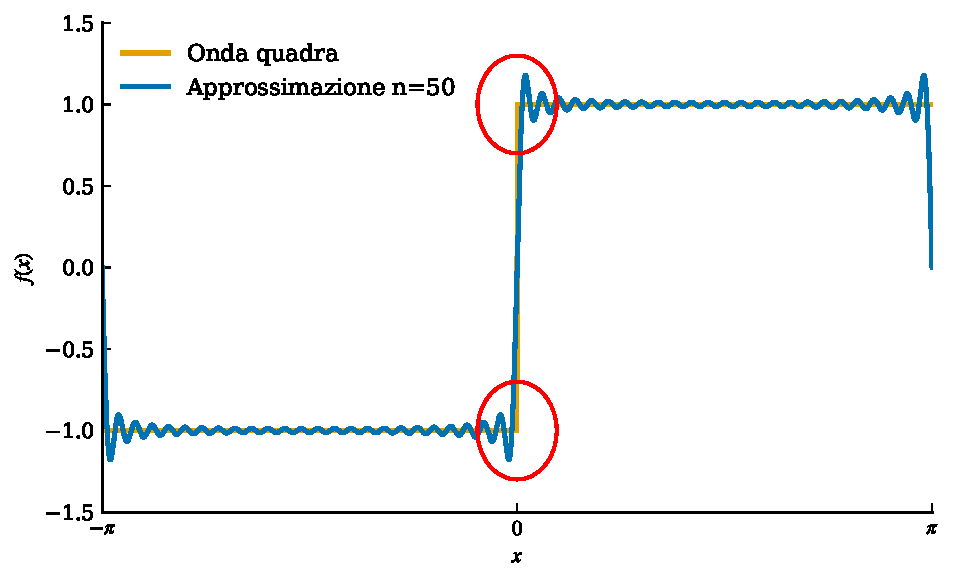
\includegraphics[width=0.5\linewidth]{Fourier_q_Gibbs.pdf}\hfill
    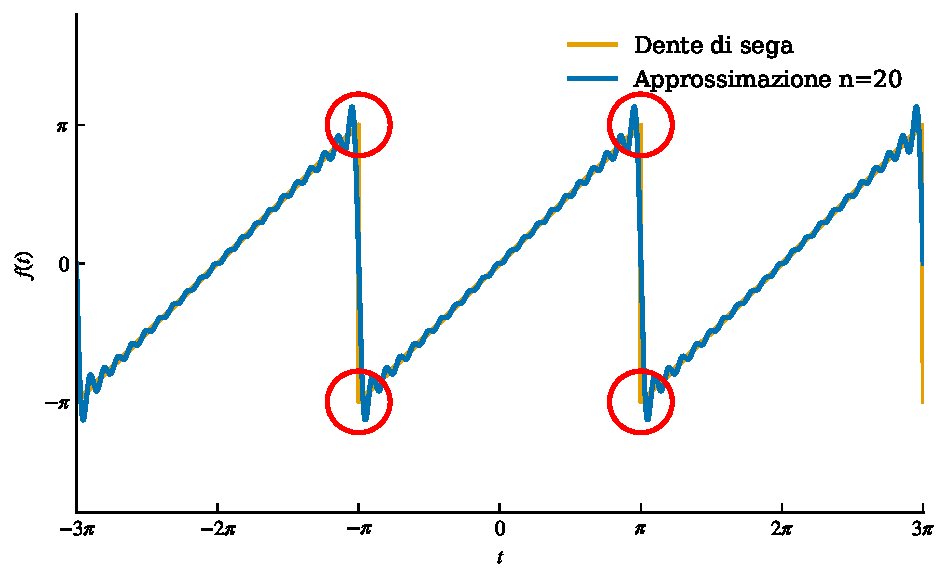
\includegraphics[width=0.5\linewidth]{Fourier_ds_Gibbs.pdf}
\end{figure}

Questo fenomeno, noto come fenomeno di Gibbs, si spiega a partire dal modo in cui le somme parziali ricostruiscono la funzione. Infatti, in un intorno di un punto di salto $x_0$, la somma parziale non distingue nettamente i valori della funzione sui due lati della discontinuità, ma ne effettua una sorta di media locale. Ciò dipende dal fatto che tali somme possono essere interpretate come una media pesata dei valori della funzione tramite il nucleo di Dirichlet, il quale è simmetrico e ha integrale unitario, quindi non privilegia né il lato destro né il lato sinistro del punto. Per questa ragione, nel punto di discontinuità la serie converge al valore medio dei limiti laterali $\frac{f(x_0^+)+f(x_0^-)}{2}$ e non a uno dei due valori della funzione. Tuttavia, mentre la funzione reale presenta un salto netto, l’approssimazione è costretta a passare attraverso valori intermedi: per colmare questa differenza locale, le somme parziali sviluppano oscillazioni attorno al punto di salto che non si attenuano al crescere del numero di termini. Il risultato è il caratteristico overshoot del fenomeno di Gibbs, che rappresenta quindi una conseguenza diretta del meccanismo di media locale con cui la serie realizza la convergenza puntuale.

\newpage

\chapter{\ Equazioni Differenziali}



In questo capitolo introdurremo la teoria delle equazioni differenziali alle derivate parziali (PDE), che costituiscono il linguaggio matematico con cui vengono descritti gran parte dei fenomeni fisici. Quando un sistema dipende simultaneamente da più variabili, le leggi che ne regolano l’evoluzione non possono più essere espresse in modo soddisfacente da relazioni algebriche o da equazioni differenziali ordinarie (ODE), ma richiedono un formalismo in grado di descrivere in modo locale e preciso come le grandezze varino (principalmente nello spazio e nel tempo): è proprio in questo contesto che le PDE emergono in modo naturale.
Queste equazioni costituiscono uno dei pilastri fondamentali su cui si regge la formulazione della fisica teorica. Fenomeni anche molto diversi tra loro (come la propagazione di onde su una corda, la diffusione del calore in un mezzo materiale o la distribuzione di un campo elettrico nello spazio) trovano una descrizione unitaria all’interno di questo stesso linguaggio matematico. Ancora più profondamente, alcune delle teorie fondamentali della fisica, come l’elettromagnetismo o la meccanica quantistica, sono interamente formulate in termini di equazioni di questo tipo, a testimonianza della loro natura strutturale.
Un punto cruciale è che la forma dell’equazione non è un semplice dettaglio formale, ma determina in modo diretto il comportamento qualitativo delle soluzioni. La struttura delle derivate coinvolte e il modo in cui esse interagiscono selezionano infatti il tipo di fenomeno che può emergere. In alcuni casi si ottengono soluzioni che descrivono fenomeni di propagazione, in cui una perturbazione si muove nello spazio e nel tempo mantenendo la propria identità strutturale (come accade per le onde); in altri casi si osservano processi di diffusione, in cui le variazioni iniziali si attenuano progressivamente e tendono a distribuirsi in modo sempre più uniforme; in altri ancora si descrivono configurazioni di equilibrio in cui il sistema non evolve nel tempo e la soluzione è completamente determinata dalle condizioni al contorno. In questo senso, la struttura matematica dell’equazione contiene già, in modo “codificato”, la natura del fenomeno fisico che essa rappresenta.
Nei paragrafi successivi analizzeremo tre esempi fondamentali, ciascuno rappresentativo di una di queste grandi classi di fenomeni: l’equazione delle onde, che descrive la propagazione; l’equazione di Laplace, che governa gli stati di equilibrio; e l’equazione del calore, che modella i processi diffusivi. Attraverso questi esempi verranno introdotti i principali metodi di risoluzione (come la separazione delle variabili e lo sviluppo in serie) mettendo in luce come strumenti matematici comuni siano in grado di descrivere fenomeni fisici profondamente diversi, rivelando così il legame essenziale tra struttura dell’equazione e comportamento delle soluzioni.
\\
\\ \underline{\textbf{Nota}}: In questo capitolo useremo due diverse notazioni per indicare l'operatore di derivata parziale: quella frazionaria e quella compatta,, che utilizzeremo a seconda della situazione. 
\\Definiamo quindi: $\displaystyle\frac{\partial}{\partial x}=:\partial_x; \  \frac{\partial^2}{\partial x^2}=:\partial_x^2;\  \frac{\partial^2}{\partial x\partial y}=: \partial_{xy}^2$.



\newpage

\section{Teoria generale}

In linea di principio, una equazione alle derivate parziali può contenere derivate di ordine arbitrariamente alto. Tuttavia, nella maggior parte dei modelli fisici fondamentali, l’attenzione si concentra quasi esclusivamente sulle equazioni del secondo ordine. La ragione di questa scelta non è soltanto di semplicità matematica, ma ha un’origine fisica profonda. Nei sistemi continui che derivano da principi variazionali o da leggi locali di interazione, i termini di ordine superiore compaiono tipicamente come correzioni di scala più piccola rispetto ai contributi dominanti. In particolare, quando si considera il limite continuo di sistemi discreti o si effettua uno sviluppo locale delle interazioni, i termini di ordine più alto risultano soppressi rispetto a quelli di ordine inferiore, e quindi non contribuiscono in modo essenziale alla dinamica macroscopica del sistema. In questo senso, il secondo ordine rappresenta il primo livello non banale in cui compaiono effetti di propagazione, diffusione o equilibrio. Le derivate prime descrivono tipicamente variazioni locali e flussi, mentre le derivate seconde introducono la possibilità di curvature e quindi di dinamiche più ricche, come oscillazioni e diffusione. Per questi motivi, le equazioni del secondo ordine costituiscono il quadro minimo in cui si osserva la varietà fondamentale dei comportamenti fisici descritti dalle PDE, e saranno quindi il principale oggetto di studio nelle sezioni successive.

Nel seguito ci limiteremo allo studio di equazioni alle derivate parziali in due variabili indipendenti. Questa scelta non è restrittiva dal punto di vista concettuale, ma permette di descrivere in modo chiaro la struttura essenziale delle equazioni del secondo ordine. Infatti, già nel caso bidimensionale è possibile mettere in evidenza la forma tipica dell’operatore differenziale e i meccanismi fondamentali che ne determinano il comportamento, mentre molte situazioni fisiche di interesse possono essere ricondotte a questo caso o studiate localmente come dipendenti da due variabili. Inoltre, successivamente ci concentreremo sulle equazioni lineari, che rappresentano il primo contesto in cui è possibile sviluppare una teoria generale delle soluzioni. La linearità garantisce infatti il principio di sovrapposizione: se due funzioni sono soluzioni, anche ogni loro combinazione lineare lo è. Questa proprietà consente una trattazione sistematica del problema e costituisce la base per strumenti fondamentali come lo sviluppo in serie e la decomposizione in soluzioni elementari. All’interno di questo quadro, inizieremo inoltre dallo studio del caso omogeneo, ossia il caso in cui non compaiono termini noti indipendenti dalla funzione incognita. Questo caso è particolarmente rilevante poiché descrive le proprietà intrinseche del sistema, indipendenti da forzanti esterne, e costituisce il punto di partenza naturale per un'analisi più generale. Dopo tutte queste doverose premesse possiamo cominciare.
\vspace{0.5cm}
\begin{definizione}[PDE]\label{def: 4.1}
    Sia $\varphi(x,y) :\Omega\subset\mathbb{R}^2\to \mathbb{R}$ tale che $\varphi\in C^2(\Omega)$. Definiamo equazione differenziale alle derivate parziali (PDE) di $\varphi$ (secondo le premesse fatte sopra) un'equazione della forma: $\ \displaystyle C_x\pdd{\varphi}{x}+C_y\pdd{\varphi}{y} +C_{xy}\pdm{\varphi}{x}{y}=0$. 
\end{definizione}
\vspace{0.5cm}
Notiamo che, grazie alla linearità dell’operatore di derivazione, è possibile riscrivere l’equazione precedente in forma più compatta utilizzando una notazione matriciale. In particolare, si può introdurre un vettore contenente le derivate prime rispetto alle variabili spaziali, in modo da esprimere la parte principale dell’equazione come una forma quadratica associata a una matrice dei coefficienti. Questo passaggio non è soltanto una riscrittura formale, ma permette di evidenziare in modo più chiaro la struttura dell’operatore e il ruolo dei termini misti, che vengono così ricondotti a una struttura algebrica ben definita.
\\
\\
\\Quindi $ \ \displaystyle C_{xx}\pdd{\varphi}{x}+C_{yy}\pdd{\varphi}{y} +C_{xy}\pdm{\varphi}{x}{y}=\bigg[\begin{pmatrix}
    \partial_x & \partial_y
\end{pmatrix}\begin{pmatrix}
    C_{xx} & C_{xy}\backslash2\\
    C_{xy}\backslash2 & C_{yy}
\end{pmatrix}\begin{pmatrix}
    \partial_x\\
    \partial_y
\end{pmatrix}\bigg]\varphi=0$
\\
\\
\\Questa riscrittura evidenzia che la struttura dell’equazione è completamente determinata da una matrice simmetrica associata ai coefficienti delle derivate seconde. L’uso di una tale rappresentazione non introduce nuovi contenuti, ma permette di ricondurre lo studio dell’operatore a problemi di algebra lineare su forme quadratiche. In particolare, eventuali cambi di variabili lineari nel piano $(x,y)$ si traducono in trasformazioni della matrice dei coefficienti, rendendo possibile una semplificazione della sua struttura. Questo punto sarà fondamentale nella classificazione delle equazioni del secondo ordine e nella riduzione alle forme canoniche.

\vspace{0.5cm}

\begin{definizione}[Notazioni utili]\label{def: 4.2}
    Per alleggerire la notazione (che in questo modo risulta molto pesante), definiamo:
    \\
    \\ 1) $\nabla_{xy} =\begin{pmatrix}
    \partial_x , \partial_y
    \end{pmatrix}$
    \\
    \\
    \\ 2) $C=\begin{pmatrix}
    C_{xx} & C_{xy}\backslash2\\
    C_{xy}\backslash2 & C_{yy}
    \end{pmatrix}$
    \\ 
    \\
    \\ 3) $\mathcal{O}=\begin{pmatrix}
    \partial_x & \partial_y
\end{pmatrix}\begin{pmatrix}
    C_{xx} & C_{xy}\backslash2\\
    C_{xy}\backslash2 & C_{yy}
\end{pmatrix}\begin{pmatrix}
    \partial_x\\
    \partial_y
\end{pmatrix}=\nabla^t_{xy}C\ \nabla_{xy}$

\end{definizione}

\vspace{0.5cm}

Notiamo subito che, mediante queste definizioni, è possibile riscrivere la PDE in forma estremamente compatta come $\mathcal{O}\varphi =0$ dove $\mathcal{O}$ rappresenta l’operatore differenziale associato alla matrice dei coefficienti. Questa notazione evidenzia in modo chiaro la struttura algebrica dell’equazione, riducendola allo studio di un operatore lineare che agisce su funzioni sufficientemente regolari (stiamo alludendo alla condizione secondo cui $\varphi\in C^2(\Omega)$). Inoltre, un eventuale cambio di coordinate nel piano, descritto da una matrice invertibile $S\in \mathbb{R}^{2\times2}$, induce una trasformazione della struttura dell’operatore. In particolare, la matrice dei coefficienti non rimane invariata, ma si trasforma secondo una legge di congruenza del tipo $C'=SCS^t$ da cui si ottiene un nuovo operatore differenziale $\mathcal{O}'$ costruito con la matrice trasformata $C'$. Questo punto è fondamentale perché mostra che la forma dell’equazione non è assoluta, ma dipende dal sistema di coordinate scelto. In particolare, la possibilità di semplificare la matrice dei coefficienti attraverso opportuni cambi di variabili sarà lo strumento chiave per la classificazione delle equazioni del secondo ordine.
\\
\\ \underline{\textbf{Nota}}: Nel caso in cui i passaggi sopra dovessero risultare poco scorrevoli, rimando alla sezione del capitolo 1 dedicata ai richiami di algebra lineare (\ref{sec: 1.1}).

\newpage



\subsection{Classificazione}\label{sec: 4.1.1}

Riprendendo la definizione di PDE (\ref{def: 4.1}), si osserva che, accanto ai termini puramente associati alle singole variabili indipendenti $x$ e $y$, compare anche il termine misto $\partial_{xy}^2\varphi$, che coinvolge simultaneamente entrambe le variabili. La presenza di questo termine introduce un accoppiamento tra le variazioni della funzione rispetto a $x$ e quelle rispetto a $y$: il comportamento di $\varphi$ lungo una direzione non è quindi indipendente dall’altra. Di conseguenza, la struttura dell’equazione non è separata nelle due variabili e risulta più difficile da analizzare.
\\
\\Riprendendo la notazione compatta $\mathcal{O}\varphi=0$, introdotta nel paragrafo precedente, e la matrice dei coefficienti $C$ definita in (\ref{def: 4.2}), si osserva che l’annullamento del termine misto è equivalente alla diagonalizzazione di $C$. In altre parole, la presenza o meno del termine $\partial_{xy}^2\varphi$ dipende dalla scelta del sistema di variabili e, in particolare, dalla possibilità di rappresentare l’operatore in una forma in cui le derivate seconde lungo le nuove direzioni risultino separate. L’idea naturale è quindi quella di utilizzare gli strumenti dell’algebra lineare per individuare un cambio di variabili che semplifichi la struttura dell’operatore, portando la matrice $C$ in forma diagonale.
\\È importante sottolineare che la matrice $C$ è reale e simmetrica; di conseguenza, per il teorema spettrale (\ref{thm: 1.8}) (o, nel caso reale, teorema di diagonalizzazione ortogonale), esiste sempre una base ortonormale di autovettori $(\eta,\xi)$ in cui tale matrice risulta diagonale. Questo fatto è particolarmente significativo, poiché garantisce che ogni equazione della forma (\ref{def: 4.1}) può essere ricondotta, tramite un opportuno cambio lineare di variabili $(x,y)\to(\eta,\xi)$, a una forma più semplice in cui il termine misto è nullo e l’operatore risulta disaccoppiato lungo le nuove direzioni. Vediamo ora come si traduce questo dal punto di vista operativo. 
\\
\\Data la matrice dei coefficienti $C$, definiamo $\Delta=:-4\det(C)$. Questo si rivela essere un ottimo strumento per classificare i vari tipi di PDE, poichè il suo segno è indipendente dal sistema di coordinate (riferito sempre allo spazi delle variabili). Notiamo infatti che data una trasformazione lineare di variabili $(x,y)\to(\eta,\xi)$ governata dalla matrice invertibile $P\in \mathbb{R}^{2\times 2}$ si ha che l'operatore differenziale $\mathcal{O}$ trasforma nel modo seguente:
\\
\\ \[ \nabla_{\eta\xi}=P\nabla_{xy}\implies \mathcal{O}'=\nabla_{\eta\xi}^tC\ \nabla_{\eta\xi}=\nabla_{xy}^tP^tCP\nabla_xy=:\nabla_{xy}C'\nabla_{xy} \]
\\
\\ Una trasformazione lineare delle variabili si traduce quindi in una trasformazione congruente della matrice dei coefficienti, cioè $C' = P^T C P$. Applicando il teorema di Binet, il determinante si comporta come $\det(C') = \det(P^T C P) = \det(P^T)\det(C)\det(P)$. Poiché il determinante di una matrice coincide con quello della sua trasposta, otteniamo immediatamente
$\det(C') = (\det P)^2 \det(C)$. 
\\A questo punto emerge il fatto cruciale: se $P \in \mathbb{R}^{2\times 2}$ è invertibile, allora $\det(P) \neq 0$ e quindi $(\det P)^2 > 0$. Ne segue che il determinante della matrice dei coefficienti può al massimo essere moltiplicato per un fattore positivo, ma non può mai cambiare segno.  In altre parole, non esistono trasformazioni lineari invertibili che possano invertire il segno di $\det(C)$. Questo rende il segno del determinante una quantità intrinseca della matrice e, di conseguenza, della PDE associata. Proprio per questo motivo, il segno di $\det(C)$ diventa un criterio naturale e stabile per classificare le equazioni differenziali parziali del secondo ordine: non dipende dal sistema di coordinate scelto, ma è una proprietà strutturale dell’equazione stessa.
\\
\\ \underline{\textbf{Nota}}: Ci si potrebbe chiedere perché non si utilizzi direttamente il segno del determinante della matrice dei coefficienti per classificare le PDE, introducendo invece il $\Delta$ (che, peraltro, ne inverte il segno).  La ragione è storica e concettuale: la classificazione delle PDE nasce originariamente dallo studio delle forme quadratiche associate alla matrice dei coefficienti, da cui deriva anche la nomenclatura (ellittica, parabolica, iperbolica). In questo contesto, il discriminante $\Delta = B^2 - 4AC$ emerge in modo naturale. Tuttavia, una trattazione completa in questi termini richiederebbe l’introduzione di strumenti teorici aggiuntivi che non sono essenziali per gli sviluppi successivi. Quanto mostrato sopra fornisce quindi una giustificazione alternativa: il segno di $\Delta$, essendo equivalente (a meno di un fattore costante negativo) al segno del determinante della matrice dei coefficienti, è invariante per trasformazioni lineari invertibili e quindi rappresenta un criterio ben posto per classificare le PDE.

\begin{itemize}
    \item$\boxed{\Delta \gt0}$ \underline{Equazioni iperboliche}: 
    \\
    \\ Ricordandoci che $C$ può essere sempre diagonalizzata, deduciamo che, dati gli autovalori $\lambda_1$ e $\lambda_2\implies sgn(\det(C))=sgn(\lambda_1\lambda_2)$. Quindi,dato che $\Delta\gt 0\implies \det(C)\lt0$ deduciamo che i due autovalori abbiano segno discorde. Definiamo quindi iperboliche tutte le equazioni riconducibili alla forma: 
    \[\displaystyle\lambda_1\pdd{\varphi}{x}-\lambda_2\pdd{\varphi}{y}=0\implies \pdd{\varphi}{x}-\frac{\lambda_2}{\lambda_1}\pdd{\varphi}{y}=0\]
    Mostreremo come la struttura di queste equazioni porti a soluzioni che non descrivono un semplice stato di equilibrio o una diffusione progressiva, ma un fenomeno di propagazione.


   \item $\boxed{\Delta\lt0}$ \underline{Equazioni ellittiche}:
    \\
    \\ Anche in questo caso deduciamo $\Delta\lt 0\implies \det(C)\gt 0$. Quindi sotto questa categoria rientrano le equazioni associate alla forma:
    \[\lambda_1\pdd{\varphi}{x}+\lambda_2\pdd{\varphi}{y}=0 \implies \pdd{\varphi}{x}+\frac{\lambda_2}{\lambda_1}\pdd{\varphi}{y}=0\]
    Queste equazioni si trovano a descrivere tipicamente condizioni di equilibrio; un esempio è l'equazione di Laplace utilizzata per descrivere l'equilibrio elettrostatico.


    \item $\boxed{\Delta=0}$ \underline{Equazioni paraboliche}: 
    \\
    \\ Seguendo lo stesso ragionamento: $\Delta =0\implies \det(C)=0\implies$ un autovettore nullo (il caso in cui siano nulli entrambi è banale. Queste equazioni sono quindi associate alla forma:
    \[\displaystyle\pdd{\varphi}{x}=0 \ \ ; \ \pdd{\varphi}{y}=0\]
    Tipicamente associate ai fenomeni di diffusione, come quella del calore.
   
\end{itemize}

























\newpage
\subsection{Struttura dei problemi}

Una equazione alle derivate parziali isolata, non è in generale sufficiente per determinare una soluzione unica. Come nel caso delle equazioni differenziali ordinarie, è necessario specificare ulteriori informazioni che selezionino, tra tutte le soluzioni possibili, quella fisicamente rilevante.
Queste informazioni aggiuntive sono fornite dalle condizioni iniziali e dalle condizioni al contorno.

\subsubsection{\underline{Condizioni iniziali}}

Consideriamo adesso la cerchia di funzioni a due variabili indipendenti $\varphi(x,t)$ ad una variabile generica $x$ ed una temporale $t$.

\begin{definizione}[Condizioni iniziali]
    Sia $\varphi(x,t)\in C^2$ una funzione che rispetti le caratteristiche enunciate sopra e sia $\mathcal{O}\varphi=0$ una PDE associata (\ref{def: 4.1}), sia inoltre $t_0$ un valore fissato della variabile temporale. Definiamo condizioni iniziali la coppia di valori $\varphi _0(x)=:\varphi(x,t_0)$ e $\dot{\varphi}_0(x)=:\partial_t\varphi(x,t_0)$.
\end{definizione}

Le condizioni iniziali descrivono lo stato del sistema in un dato istante $t_0$. Dal punto di vista più generale rappresentano l’informazione necessaria per selezionare una particolare traiettoria evolutiva tra tutte quelle matematicamente possibili. In particolare, nel caso di equazioni del secondo ordine nel tempo, è naturale che siano richiesti sia il valore della funzione sia quello della sua derivata temporale.
Un aspetto rilevante è che, per equazioni di tipo diverso, il ruolo delle condizioni iniziali cambia profondamente. Vedremo infatti come nel caso di equazioni che descrivono fenomeni di propagazione, come l’equazione delle onde, esse determinano la struttura dinamica delle perturbazioni. Nel caso di equazioni dissipative, come quella del calore, le condizioni iniziali vengono progressivamente “dimenticate”, poiché l’evoluzione tende a smorzare le differenze iniziali fino a raggiungere uno stato di equilibrio. Questo mette in evidenza un punto fondamentale: le condizioni iniziali non solo fissano lo stato iniziale, ma influenzano anche qualitativamente il comportamento della soluzione, interagendo in modo non banale con la struttura dell’equazione differenziale.

\subsubsection{\underline{Condizioni al contorno}}

Accanto alle condizioni iniziali, un ruolo altrettanto fondamentale è svolto dalle condizioni al contorno, che intervengono quando il problema è definito su un dominio spaziale limitato. Esse specificano il comportamento della soluzione sul bordo del dominio e risultano essenziali per determinare in modo univoco la soluzione del problema.

\begin{definizione}[Condizione al contorno]
    Sia $\varphi:\Omega \subset\mathbb{R}^2\to \mathbb{R}$, $\varphi \in C^2(\Omega)$ e $\mathcal{O}\varphi=0$ una PDE. Inoltre sia $\Omega$ limitato e $\partial\Omega$ il suo bordo. Le condizioni a contorno sono vincoli assegnati alla funzione incognita $\varphi$ (o alle sue derivate) ristretti ai punti del bordo $\partial\Omega$. 
    \\ 
    \\Più precisamente si possono esprimere attraverso $\mathcal{B}_{\partial\Omega}[\varphi]=g$, dove $\mathcal{B}_{\partial\Omega}$ è un operatore ristretto a $\partial\Omega$ e $g$ è una funzione assegnata su $\partial\Omega$.
\end{definizione}

Dal punto di vista fisico, le condizioni al contorno descrivono il tipo di interazione tra il sistema e il suo ambiente attraverso la frontiera del dominio. In altre parole, non riguardano l’evoluzione interna del fenomeno, ma il modo in cui esso è vincolato o influenzato ai suoi estremi spaziali (si fa naturalmente riferimento ad un bordo spaziale fisico o ad un bordo sulle condizioni inteso in senso astratto). La scelta delle condizioni al contorno determina quindi il comportamento del sistema in prossimità del bordo e, in particolare, stabilisce quali grandezze fisiche risultano controllate o imposte dall’esterno, influenzando in modo essenziale la forma globale della soluzione. Vediamo alcuni esempi famosi.
\vspace{0.5cm}
\begin{definizione}[Condizioni di Dirichlet]\label{def: 4.5}
    Date le stesse ipotesi della definizione generale, si definiscono condizioni a contorno di Dirichlet: $\varphi|_{\partial\Omega}=f$.
\end{definizione}
\vspace{0.5cm}
Ii questo caso si assegna direttamente il valore della grandezza fisica sul bordo del dominio tramite la funzione $f$. Ad esempio, nel caso della diffusione del calore, questo corrisponde a mantenere fissata la temperatura agli estremi di un corpo; nel caso di una corda vibrante, equivale a imporre che gli estremi siano bloccati.
\vspace{0.5cm}
\begin{definizione}[Condizioni di Neumann]
    Date le stesse ipotesi della definizione principale si definiscono le condizioni al contorno di Neumann: $\displaystyle\frac{\partial\varphi}{\partial n}\bigg|_{\partial\Omega}=g$, dove $n$ è la direzione normale a $\partial\Omega$.
\end{definizione}
\vspace{0.5cm}
Riprendendo l'esempio della diffusione, la condizione di Neumann rappresenta un flusso termico assegnato attraverso il bordo governato dalla funzione $g$. Segue anche che, in tale contesto, la condizione $\partial_n\varphi=0$ impone uno scambio di calore nullo con l'ambiente circostante.
\vspace{0.5cm}
\begin{definizione}[Condizioni miste]
    Date le stesse ipotesi della definzione generale, di definiscono condizioni miste: $a\varphi+b\displaystyle\frac{\partial\varphi}{\partial n}=h; \ \ a,b\in \mathbb{R}$.
\end{definizione}
\vspace{0.5cm}
Queste condizioni più generali descrivono situazioni intermedie in cui il sistema interagisce con l’ambiente circostante in modo più realistico, ad esempio attraverso scambi proporzionali tra il valore della grandezza e il suo flusso attraverso il bordo.
\\
\\In definitiva, le condizioni al contorno non sono un elemento accessorio, ma parte integrante di un problema fisico. Esse determinano in modo sostanziale la forma della soluzione e, insieme all’equazione differenziale, rendono il problema matematicamente ben posto.
\\
\\A questo punto siamo davvero pronti per entrare nel vivo della trattazione. Nelle prossime sezioni analizzeremo con attenzione i tre casi fondamentali di PDE e, passo dopo passo, costruiremo un metodo generale di risoluzione. Questo ci permetterà di affrontare con sicurezza e consapevolezza i principali problemi fisici espressi attraverso questo linguaggio.

\newpage

\section{Equazione delle Onde}

Tra le equazioni differenziali alle derivate parziali, l’equazione delle onde occupa un ruolo centrale sia dal punto di vista matematico che fisico. Essa descrive in modo efficace tutti quei fenomeni in cui una perturbazione si propaga nello spazio e nel tempo mantenendo, almeno localmente, una propria identità dinamica. Stiamo parlando di un'equazione di tipo iperbolico che, a differenza di altri tipi di equazioni che tendono a descrivere processi di rilassamento o stati di equilibrio, introduce naturalmente il concetto di propagazione a velocità finita dell'informazione.
Un aspetto fondamentale è che la struttura dell’equazione non si limita a determinare l’evoluzione quantitativa del sistema, ma ne condiziona profondamente il comportamento qualitativo. La forma delle derivate coinvolte stabilisce infatti se una perturbazione si muove, si attenua o si stabilizza nel tempo. In questo senso, l’equazione delle onde rappresenta il prototipo dei fenomeni di propagazione: una volta introdotta una deformazione iniziale, questa non si dissolve immediatamente, ma si trasmette nello spazio attraverso due direzioni privilegiate. Dal punto di vista matematico, questa equazione emerge in modo naturale in contesti molto diversi tra loro, ma accomunati dalla presenza di leggi locali e lineari. Il fatto che sistemi fisici apparentemente lontani condividano la stessa struttura differenziale evidenzia un principio più profondo: non è il contenuto fisico specifico a determinare la forma dell’equazione, ma la combinazione tra simmetrie, linearità e interazioni locali del sistema.
In questa sezione vedremo come la sua struttura permetta una soluzione esatta in termini di onde che si propagano indipendentemente verso destra e verso sinistra. Successivamente analizzeremo il ruolo delle condizioni iniziali e al contorno, che non si limitano a selezionare una soluzione tra molte, ma influenzano direttamente la forma globale della dinamica. Infine, vedremo come questa equazione possa essere derivata da modelli microscopici discreti nel limite continuo. 

\begin{definizione}[Equazione delle onde]\label{def: 4.8}
    Sia $\varphi(x,t): \Omega\subseteq\mathbb{R}^2\to \mathbb{R}$ una funzione sufficientemente regolare (quindi almeno $C^2(\Omega)$) e sia $v\gt 0$. L'equazione delle onde è una PDE di tipo iperbolico (\ref{sec: 4.1.1}) della forma: $\displaystyle\pdd{\varphi}{t}-v^2\pdd{\varphi}{x}=0$.
\end{definizione}

\underline{\textbf{Nota}}: Tipicamente i parametri $x,t$ hanno le dimensioni di uno spazio e di un tempo e $v$ di una velocità. Tuttavia, essendo questi degli appunti di matematica, considereremo tali grandezze adimensionali e a valori in $\mathbb{R}$ di modo da coprire una trattazione più generale dal punto di vista formale. Nonostante ciò ci si riferirà ai parametri come "spazio","tempo" e "velocità" per evitare una nomenclatura eccessivamente pesante.

\begin{definizione}[Operatore D'Alembertiano]
    Definiamo l'operatore differenziale D'Alembertiano nel modo seguente: $\Box=:[\partial_t^2-v^2\partial_x^2]$.
    \\
    \\A seconda dei contesti lo si può trovare in varie forme come nel caso di più parametri spaziali ($\nabla^2-v^2\partial_t^2$) o nella notazione covariante ($g^{\mu\nu}\nabla_\mu\nabla_\nu$).
\end{definizione}

Si nota immediatamente che l'equazione delle onde si può riscrivere in forma molto più compatta utilizzando l'operatore D'Alembertiano appena introdotto, infatti:
\[\displaystyle\pdd{\varphi}{t}-v^2\pdd{\varphi}{x}=0\iff \Box\varphi=0\]

\newpage

Un aspetto fondamentale da sottolineare prima di andare avanti è che l'equazione delle onde è lineare nelle soluzioni.

\begin{proposizione}\label{prop: 4.1}
    L'equazione delle onde (\ref{def: 4.8}) è lineare nelle soluzioni.
    \\
    \\\underline{Dimostrazione}: Siano $\phi_1$ e $\phi_2$ soluzioni dell'equazione delle onde e notiamo che una generica combinazione lineare $\lambda\phi_1+\mu\phi_2$ è soluzione.\\
    \\ Infatti: $\partial_t^2(\lambda\phi_1+\mu\phi_2)-v^2\partial_x^2(\lambda\phi_1+\mu\phi_2)=\lambda\Box\phi_1+\mu\Box\phi_2=0$.\qed
\end{proposizione}

Questo risultato, apparentemente elementare, ha in realtà conseguenze strutturali rilevanti. La linearità dell’equazione implica infatti che l’insieme delle sue soluzioni non sia soltanto un insieme, ma un sottospazio vettoriale reale dello spazio delle funzioni sufficientemente regolari.Inoltre abbiamo anche mostrato come l'operatore D'Alembertiano sia lineare. Questa struttura permette di introdurre in modo naturale il principio di sovrapposizione, secondo cui soluzioni elementari dell’equazione possono essere combinate linearmente per costruire soluzioni più generali. Tale proprietà sarà alla base di tutti i metodi di risoluzione che verranno introdotti nelle sezioni successive.

Questa proprietà assume un ruolo ancora più significativo quando si osserva che, per l’equazione delle onde, le soluzioni non solo possono essere combinate linearmente, ma ammettono una descrizione in termini di onde elementari. In altre parole, la linearità dell’operatore implica che ogni soluzione può essere costruita come sovrapposizione di contributi più semplici, ciascuno dei quali rappresenta una perturbazione che si propaga indipendentemente nello spazio. Questo suggerisce che la struttura generale delle soluzioni non è arbitraria, ma organizzata a partire da configurazioni fondamentali che evolvono secondo dinamiche di propagazione. Sarà proprio questa osservazione a guidare la costruzione esplicita della soluzione generale dell’equazione, che verrà espressa come somma di onde che si propagano in direzioni opposte.

\subsection{Soluzione di D'Alembert: caso generale}\label{sec: 4.2.1}

Forniamo adesso un primo metodo risolutivo per l'equazione delle onde: la soluzione di D'Alembert. Per prima cosa notiamo che l'operatore D'Alembertiano è fattorizzabile nel modo seguente:
\[\Box =\partial_t^2-v^2\partial_x^2=(\partial_t+v\partial_x)(\partial_t-v\partial_x)\]
Queste costituiscono un cambio di coordinate particolarmente adatto allo studio dell’equazione, poiché trasformano le direzioni lungo cui agiscono gli operatori del primo ordine in variabili indipendenti, lungo le quali l’equazione si semplifica e non vi è più accoppiamento tra le derivate rispetto a spazio e tempo.
Introduciamo quindi il seguente cambio di coordinate:

\[
\begin{cases}
\eta = x - vt \\
\xi = x + vt
\end{cases}
\qquad \iff \qquad
\begin{cases}
x = \dfrac{\xi + \eta}{2} \\
t = \dfrac{\xi - \eta}{2v}
\end{cases}
\]
\\
\\In questo senso il sistema realizza una trasformazione lineare invertibile sul piano $(x,y)$, la cui matrice jacobiana diagonalizza la struttura dell’operatore d’Alembertiano, permettendone la riduzione a una forma differenziale separabile nelle variabili $(\eta,\xi)$.

\newpage

\begin{proposizione}
    Sia $\varphi(x,y)\in C^2(\Omega)$. Considerando il cambio di coordinate definito come $\eta=x-vt, \ \xi=x+vt$, si ha la seguente trasformazione dell'equazione d'onda: 
    \[\partial_t^2\varphi-v^2\partial_x^2\varphi=-4v^2\partial_{\eta\xi}^2\varphi\]
    \\\underline{Dimostrazione}: La trasformazione è governata dalla matrice jacobiana definita come:
    \\ 
    \\$J=\begin{pmatrix}
        \pd{\eta}{x}&\pd{\eta}{t}
        \\
    \\  \pd{\xi}{x}&\pd{\xi}{t}
    \end{pmatrix}=\begin{pmatrix}
        1&-v
        \\1&v
    \end{pmatrix}\implies \nabla_{xt}=J^t\nabla_{\eta\xi}\implies \partial_x=\partial_\eta+\partial_\xi \ ; \ \partial_t=v(\partial_\xi-\partial_\eta)$.
    \\ 
    \\ Notiamo adesso che possiamo riscrivere il D'Alembertiano come: $\Box=\nabla_{xt}^t\begin{pmatrix}
        -v^2&0
        \\0&1
    \end{pmatrix}\nabla_{xt}$.
    \\
    \\ Quindi $\Box=(J^t\nabla _{\eta\xi})^t\begin{pmatrix}
        -v^2&0
        \\0&1
    \end{pmatrix}(J^t\nabla _{\eta\xi})=\nabla_{\eta\xi}^t\bigg[J\begin{pmatrix}
        -v^2&0
        \\0&1
    \end{pmatrix}J^t\bigg]\nabla_{\eta\xi}=\nabla_{\eta\xi}^t\bigg[-4v^2\begin{pmatrix}
        0&1
        \\1&0
    \end{pmatrix}\bigg]\nabla_{\eta\xi}$
    \\
    \\
    \\$=-4v^2\partial_{\eta\xi}^2\implies\Box\varphi=-4v^2\partial_{\eta\xi}^2\varphi$.\qed 
\end{proposizione}

Quindi nelle coordinate $(\eta,\xi)$, l'equazione delle onde assume una forma più compatta: \[\Box\varphi=0\implies-4v^2\partial_{\eta\xi}^2\varphi=0\implies \partial_{\eta\xi}^2\varphi=0\implies \partial_\eta(\partial_\xi\varphi)=\partial_\xi(\partial_\eta\varphi)=0\]
Questa rappresentazione risulta significativamente più semplice rispetto alla formulazione originale, poiché l’operatore differenziale si riduce ad una sola derivata mista del secondo ordine. In particolare, l’equazione non coinvolge più derivate seconde pure rispetto alle singole variabili $\eta$ e $\xi$, rendendo possibile un’integrazione diretta.
\\
\\In particolare, la relazione $\partial_\eta(\partial_\xi\varphi)=0$ impone un vincolo strutturale molto forte: la quantità $\partial_\xi\varphi$ ha derivata nulla rispetto a $\eta$, quindi non può dipendere da essa. Ne segue che $\partial_\xi\varphi$ è funzione della sola variabile $\xi$, cioè esiste una funzione $g(\xi)$ tale $\partial_\xi\varphi=g'(\xi)$.
Similmente, $\partial_\xi(\partial_\eta\varphi)$ implica che $\partial_\eta\varphi$ non dipenda da $\xi$, e quindi esiste una funzione $f(\eta)$ tale che $\partial_\eta\varphi=f'(\eta)$. 
\\Integrando rispetto alle variabili corrispondenti si ottengono quindi due contributi indipendenti della soluzione: $\varphi=f(\eta), \ \ \varphi=g(\xi)$. Questi rappresentano le due famiglie fondamentali di soluzioni dell’equazione delle onde in coordinate caratteristiche. In particolare, $f(\eta)=f(x-vt)$ descrive una componente della soluzione costante lungo le rette $x-vt=cost.$, mentre $g(\xi)=g(x+vt)$ descrive una componente costante lungo le rette $x+vt=cost.$. In entrambi i casi si tratta di profili che si traslano rigidamente nello spazio-tempo (o più precisamente nello spazio delle variabili) senza deformazione.
\\Poiché lo spazio delle soluzioni è lineare (proposizione~\ref{prop: 4.1}), ogni combinazione lineare di tali soluzioni è ancora soluzione. Questo fatto non è soltanto tecnico, ma ha un significato fisico preciso: l’equazione non introduce interazione tra i due modi di propagazione, che rimangono indipendenti.Si ottiene quindi la forma generale:

\[\varphi(\eta,\xi)=\lambda f(\eta)+\mu g(\xi)\iff \varphi(x,y)=\lambda f(x-vt)+\mu g(x+vt)\]

Questa decomposizione mette in evidenza la struttura fondamentale dell’equazione delle onde: ogni soluzione può essere interpretata come sovrapposizione di due onde elementari che si propagano lungo le direzioni caratteristiche, senza deformarsi e senza interagire tra loro. 

\subsubsection{\underline{Interpretazione grafica}}

Un esempio classico di soluzione dell’equazione delle onde nella forma di D’Alembert è quello dei pacchetti d’onda gaussiani. Ossia funzioni della forma: 

\[
f(x,t) = \exp\!\left(-\frac{(x \pm vt)^2}{2\sigma^2}\right)\iff f(\eta)=\exp\!\left(-\frac{\eta^2}{2\sigma^2}\right), \ g(\xi)=\exp\!\left(-\frac{\xi^2}{2\sigma^2}\right)
\]
\\che descrivono una gaussiana centrata in $x=\pm vt$ al variare del parametro temporale. Come esercizio, si può verificare che questa famiglia di funzioni soddisfa l’equazione delle onde, perché dipende solo dalle variabili $(\eta,\xi)$.Di seguito sono mostrati due pacchetti gaussiani che si propagano lungo queste direzioni caratteristiche. La prima immagine mostra il caso in cui i due contributi si sommano (interferenza costruttiva), mentre la seconda mostra il caso in cui si sottraggono (interferenza distruttiva).

\begin{figure}[H]
    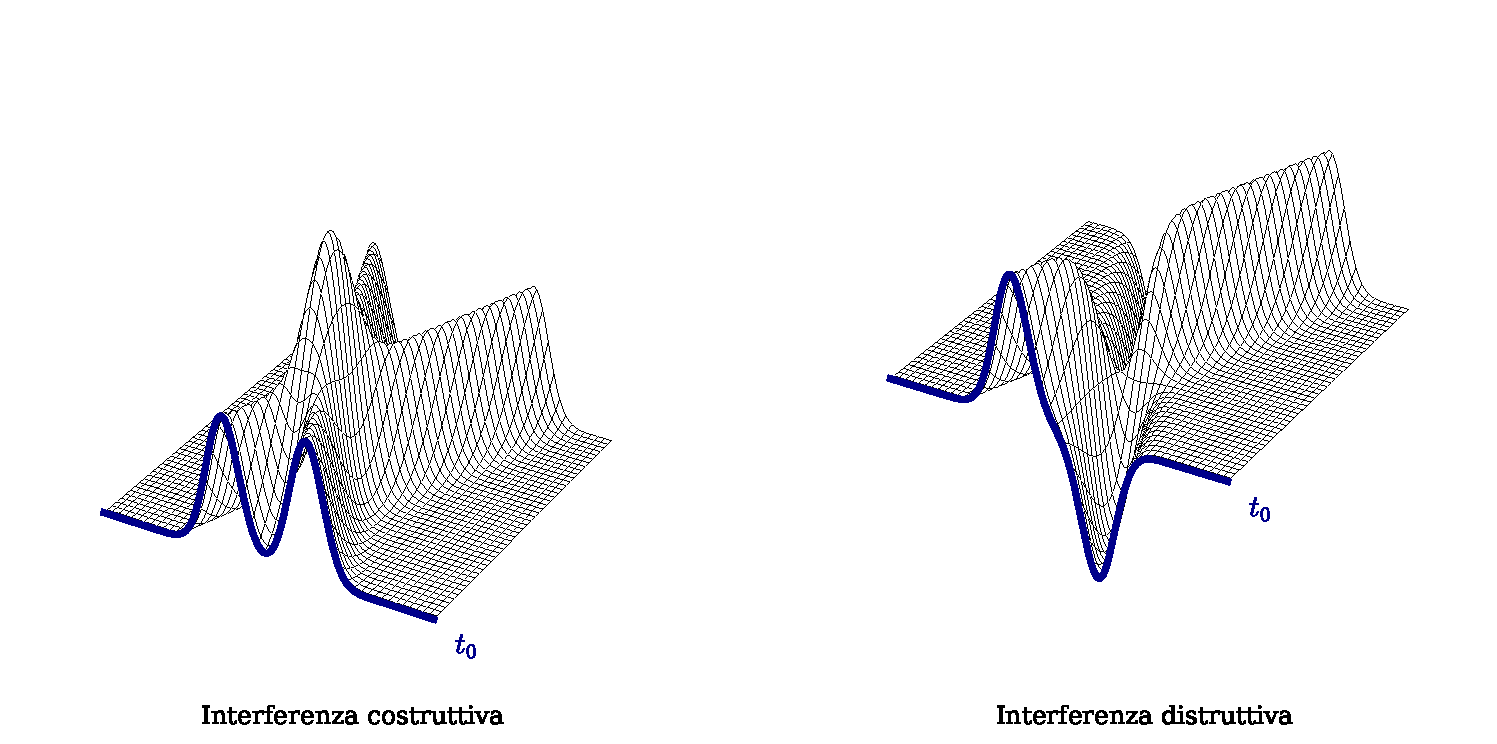
\includegraphics[width=1\linewidth]{DAlambert_sec_1.pdf}
\end{figure}

In entrambi i casi si osservano due pacchetti gaussiani identici che si propagano lungo le direzioni caratteristiche del sistema $(\eta,\xi)$. 
Un aspetto importante riguarda l’interpretazione del grafico. La superficie rappresenta la funzione $\varphi(x,t)$, cioè il campo come funzione congiunta di spazio e tempo. In questo senso non si tratta direttamente di una “forma dell’onda” in un istante fissato, ma di una descrizione completa dell’evoluzione temporale del sistema. In termini semplici: quella che vedete non è l'onda nel senso spaziale del termine.
Tuttavia, fissando un valore del tempo $t=t_0$, la sezione della superficie nel piano $\varphi(x,t_0)$ fornisce proprio la configurazione dell’onda a quell’istante. In altre parole, ogni taglio orizzontale della superficie a tempo costante rappresenta una funzione monodimensionale $\varphi(x,t_0)$, che corrisponde alla forma dell’onda nello spazio in quel preciso momento. La superficie tridimensionale può quindi essere vista come l’insieme continuo di queste configurazioni istantanee al variare del tempo.
La differenza tra le due immagini riguarda il modo in cui i due contributi si combinano: nel primo caso si sommano dando interferenza costruttiva nella regione di sovrapposizione, mentre nel secondo caso si sottraggono generando interferenza distruttiva. In entrambi i casi rimangono invariati i due elementi fondamentali della dinamica: la propagazione lungo le caratteristiche e la linearità dell’equazione, che consente la sovrapposizione delle soluzioni.

\newpage

\subsection{Soluzione di D'Alembert: condizioni assegnate}

In questo paragrafo completeremo la costruzione della soluzione di D'Alembert dell’equazione delle onde nel caso fisicamente rilevante di una condizione inizile fissata e di un dominio finito. A partire dalla forma delle soluzioni già ottenuta per il problema su $\mathbb{R}$, mostreremo come le condizioni iniziali determinino le due componenti d’onda e come, nel caso di un intervallo limitato, le condizioni al contorno non modifichino la struttura della soluzione, ma impongano invece un’opportuna estensione dei dati iniziali al di fuori del dominio fisico. In questo modo il problema su $x\in [0,L]$ viene ricondotto a un problema equivalente su tutto $\mathbb{R}$, in cui la soluzione conserva la forma generale già nota, ma incorpora implicitamente gli effetti delle riflessioni ai bordi.

\subsubsection{\underline{Condizioni iniziali}}

Consideriamo adesso l'equazione delle onde affiancata dai valori della funzione incognita ad un istante $t_0$ fissato, nonchè il valore della sua derivata prima temporale sempre calcolata all'istante $t_0$ fissato. È importante sottolineare che, a differenza del caso delle equazioni differenziali ordinarie studiate al corso di Analisi 1, le condizioni iniziali non sono valori numerici ma funzioni dello spazio, in particolare $\varphi (x,t_0)$ rappresenta la forma della funzione all'istante iniziale e $\partial_t\varphi(x,t_0)$ la sua velocità punto per punto nel medesimo istante. Ci ritroviamo quindi con il seguente problema di Cauchy:
\[\begin{cases}
    \partial_t^2\varphi(x,t)-v^2\partial_x^2\varphi(x,t)=0\iff \Box\varphi(x,t)=0
    \\ \varphi_0(x)=\varphi(x,t_0)
    \\ \dot{\varphi}_0(x)=\partial_t\varphi(x,t_0)
\end{cases}\]
Consideriamo la soluzione trovata nel paragrafo precedente (ponendo le costanti $\lambda,\mu=1$ per non appesantire ulteriormente la notazione) nella forma:
\[\varphi(x,t)=f(x-v(t-t_0))+g(x+v(t-t_0))\]
\underline{\textbf{Nota}}: Bisogna tenere bene a mente che le funzioni $f(x-v(t-t_0))$ e $g(x+v(t-t_0))$ non sono funzioni di due parametri indipendenti $(x,t)$ ma di un unico parametro, infatti $f=f(\eta), g=g(\xi)$. Per questo motivo si avrà: 
\[\partial_t\varphi(x,t)=\partial_tf(\eta(x,t))+\partial_tg(\xi(x,t))=\displaystyle\frac{df}{d\eta}\partial_t\eta(x,t)+\frac{dg}{d\xi}\partial_t\xi(x,t)=f'(-v)+g'(v)
\]
\[\partial_x\varphi(x,t)=\partial_xf(\eta(x,t))+\partial_xg(\xi(x,t))=\displaystyle\frac{df}{d\eta}\partial_x\eta(x,t)+\frac{dg}{d\xi}\partial_x\xi(x,t)=f'+g'\]
Alla luce di questo notiamo che, ponendo $t=t_0\implies \tau=t-t_0=0$, valgono le seguenti relazioni:
\[\varphi_0(x)=f(x)+g(x) \ \ \ ,\ \ \ \dot{\varphi}_0(x)=-vf'(x)+vg'(x)\ \ \ , \ \ \varphi'_0(x)=f'(x)+g'(x)\]
Risolvendo per $f'$ e $g'$ ci ritroviamo con le seguenti relazioni:
\[f'(x)=\displaystyle\frac{1}{2}\bigg(\varphi'_0(x)-\frac{1}{v}\dot{\varphi}_0(x)\bigg)\ \ \ , \ \ \ g'(x)=\frac{1}{2}\bigg(\varphi'_0(x)+\frac{1}{v}\dot{\varphi}_0(x)\bigg) \]
Notiamo quindi che il problema è quasi risolto: infatti, integrando le espressioni sopra ci ritroveremo con delle formule operative per calcolare le funzioni che compongono la soluzione generale del problema modellate sui parametri iniziali.

\newpage

\underline{\textbf{Nota}}: Nella nota precedente abbiamo sottolineato il fatto che le funzioni $f, g$ fossero dipendenti da una sola variabile indipendente e per tanto, le derivate sono state calcolate secondo la regola della derivazione a catena. Tuttavia, le espressioni che dobbiamo integrare (essendo state calcolate in $t-t_0=0$) sono funzioni della sola variabili spaziale e quindi è pertinente operare un'integrazione rispetto a suddetta variabile.
\\
\\ Quindi: $\begin{cases}f(x)=\displaystyle\frac{1}{2}\int_0^x\bigg(\varphi'_0(z)-\frac{1}{v}\dot{\varphi}_0(z)\bigg)\,dz=\frac{\varphi_0(x)}{2}-\frac{1}{2v}\int_0^x\dot{\varphi}_0(z)\,dz
    \\
    \\g(x)=\displaystyle\frac{1}{2}\int_0^x\bigg(\varphi'_0(z)+\frac{1}{v}\dot{\varphi}_0(z)\bigg)\,dz=\frac{\varphi_0(x)}{2}+\frac{1}{2v}\int_0^x\dot{\varphi}_0(z)\,dz
\end{cases}$.
\\
\\
\\Le funzioni $f(x)$ e $g(x)$ sono completamente determinate dai dati iniziali e dipendono esclusivamente dalla variabile spaziale. Il tempo non compare nella loro definizione, ma entra solo successivamente attraverso la composizione con gli argomenti traslati $x\pm v\tau$, che descrivono la propagazione dinamica delle onde. Una volta fissate tali funzioni, infatti, l’evoluzione temporale consiste esclusivamente nella loro traslazione lungo le direzioni caratteristiche $x\pm v\tau$, senza introdurre nuove dipendenze funzionali. 
\\
\\ Segue: $f(x-v(t-t_0))=\displaystyle\frac{\varphi_0(x-v(t-t_0))}{2}-\frac{1}{2v}\int_0^{x-v(t-t_o)}\dot{\varphi}_0(z)\,dz$, e similmente deduciamo anche $g(x+v(t-t_0))=\displaystyle\frac{\varphi_0(x+v(t-t_0))}{2}+\frac{1}{2v}\int_0^{x+v(t-t_o)}\dot{\varphi}_0(z)\,dz$.
\\
\\Sommando le due soluzioni, troviamo quindi la forma generale della soluzione dell'equazione delle onde con parametri iniziali:
\[\varphi(x,t)=\displaystyle\frac{1}{2}\bigg[\varphi_0(x-v(t-t_0))+\varphi_0(x+v(t-t_0))\bigg]+\frac{1}{2v}\int_{x-v(t-t_0)}^{x+v(t-t_0)}\dot{\varphi}_0(z)\,dz\]
La soluzione di D’Alembert per l’equazione delle onde su $\mathbb{R}$, con dati iniziali assegnati a $t=t_0$ che ci siamo appena ricavati, mostra che l’evoluzione del campo $\varphi(x,t)$ è completamente determinata dai dati di Cauchy calcolati al tempo iniziale $t_0$ senza introdurre nuove dipendenze funzionali. La struttura della soluzione evidenzia che il tempo compare solo attraverso la combinazione $(t-t_0)$, riflettendo l’invarianza per traslazioni temporali. Ne segue che l’evoluzione dipende solo dall’intervallo di tempo trascorso rispetto all’istante iniziale e non dalla scelta assoluta dell’origine dei tempi. Una volta assegnati i dati iniziali, il problema risulta quindi completamente deterministico e ben posto. Questo aspetto è rilevante perché implica che non esista un istante temporale privilegiato nella dinamica: qualsiasi scelta di $t_0$ conduce alla stessa evoluzione, semplicemente parametrizzata in modo diverso.
\\Dal punto di vista fisico, il risultato descrive correttamente fenomeni di propagazione ondosa in regime lineare e non dissipativo, come onde su una corda ideale o onde acustiche in un mezzo perfetto. In tali sistemi, le perturbazioni iniziali si propagano con velocità finita lungo il mezzo, senza attenuazione né dispersione intrinseca, ma mediante trasporto della configurazione iniziale lungo le direzioni caratteristiche del problema.

\newpage

\subsubsection{\underline{Condizioni a contorno}}

Nel caso di un dominio illimitato, i dati iniziali $\varphi_0(x)$ e $\dot{\varphi}_0(x)$ risultano definiti su tutto $\mathbb{R}$, e la formula di D’Alembert determina direttamente la soluzione. La situazione cambia invece quando il sistema è definito in un intervallo finito $[0,L]$, poiché la presenza di estremi impone l’introduzione di condizioni al contorno. In questo caso, le condizioni iniziali sono assegnate solo nell’intervallo fisico $[0,L]$, mentre la soluzione di D’Alembert coinvolge valori delle funzioni iniziali valutati nei punti $x\pm v(t-t_0)$, che possono uscire dal dominio. Diventa quindi necessario stabilire un prolungamento delle condizioni iniziali al di fuori dell’intervallo fisico, in modo compatibile con le condizioni al contorno imposte agli estremi del sistema.
\\
\\ Consideriamo quindi l'equazione delle onde definita su un dominio spaziale $[0,L]$ con condizioni al contorno di Dirichlet (\ref{def: 4.5}) $\varphi(0,t)=0$ e $\varphi(L,t)=0$. Consideriamo inoltre delle condizioni iniziali. Ci ritroviamo quindi con un problema della forma:
\[\begin{cases}
    \partial_t^2\varphi(x,t)-v^2\partial_x^2\varphi(x,t)=0\iff \Box\varphi(x,t)=0
    \\\varphi_0(x)=\varphi(x,t_0)
    \\\dot{\varphi}_0(x)=\partial_t\varphi(x,t_0)
    \\\varphi(0,t)=0
    \\\varphi(L,t)=0
\end{cases}\]
Il prolungamento dei dati iniziali nasce dal fatto che la soluzione di D’Alembert coinvolge i termini $\varphi_0(x\pm v\tau)$ e $\dot{\varphi}(x\pm v\tau)$ i cui argomenti, durante l’evoluzione temporale, possono uscire dall’intervallo $[0,L]$. Tuttavia, le condizioni iniziali sono definite solo all’interno di tale intervallo, per cui la formula non sarebbe più direttamente utilizzabile. Per risolvere il problema, si introduce allora un’estensione concettuale: si immagina che le funzioni iniziali siano definite anche al di fuori dal dominio $[0,L]$, costruendo un prolungamento matematico compatibile con le condizioni al contorno. In questo modo si può continuare a usare la forma generale della soluzione di D’Alembert come se il sistema fosse definito su tutta la retta, facendo però in modo che la soluzione soddisfi automaticamente i vincoli agli estremi.
\begin{itemize}
    \item \underline{Prolungamento di $\varphi_0(x)$}: La parte della soluzione di D'Alembert che coinvolge $\varphi_0(x)$ è: $\varphi(x,\tau)=\displaystyle\frac{1}{2}[\varphi_0(x-v\tau)+\varphi_0(x+v\tau)]$. Imponendo $\varphi(0,\tau)=0$ otteniamo:
    \[\varphi(0,\tau)=\frac{1}{2}[\varphi_0(-v\tau)+\varphi_0(v\tau)]=0\implies \varphi_0(-v\tau)=-\varphi_0(v\tau)\iff\varphi_0(-z)=-\varphi_0(z)\]
    Questa relazione ci suggerisce che $\varphi_0$ deve essere prolungata come funzione dispari rispetto all'esterno. Imponiamo adesso la condizione $\varphi(L,t)=0$. Seguendo dei passaggi analoghi a quelli sopra ci ritroviamo con la relazione:
    \[\varphi_0(L-z)=-\varphi_0(L+z)\]
    Quindi il prolungamento di $\varphi_0$ deve essere dispari anche rispetto al punto $x=L$. Combinando le due richieste, $\varphi_0$ dovrà essere estesa fuori dall’intervallo fisico $[0,L]$ come funzione dispari e periodica di periodo $2L$. In questo modo la soluzione costruita tramite la formula di D’Alembert soddisfa automaticamente le condizioni al contorno per ogni valore di $\tau$. Dal punto di vista geometrico, il prolungamento dispari introduce una riflessione con inversione di segno ogni volta che l’onda raggiunge un estremo del dominio.
    
    \item\underline{Prolungamento di $\dot{\varphi}_0(x)$}: Nella soluzione generale di D'Alembert, l'unico termine contenente $\dot{\varphi}_0(x)$ è: $\varphi(x,\tau)=\displaystyle\frac{1}{2v}\int_{x-v\tau}^{x+v\tau}\dot{\varphi}_0(z)\,dz$. Imponendo nuovamente le condizioni al bordo di Dirichlet, troviamo le seguenti relazioni:
    \[\begin{cases}\displaystyle\varphi(0,\tau)=\frac{1}{2v}\int_{-v\tau}^{v\tau}\dot{\varphi}_0(z)\,dz=0\implies\dot{\varphi}_0(-z)=-\dot{\varphi}_0(z)
    \\
    \\\displaystyle\varphi(L,\tau)=\frac{1}{2v}\int_{L-v\tau}^{L+v\tau}\dot{\varphi}_0(z)\,dz=0\implies\dot{\varphi}_0(L-z)=-\dot{\varphi}_0(L+z)
        \end{cases}\]
    Questo perchè, affinché l'integrale sia nullo, la funzione integranda deve essere dispari sul dominio di integrazione.


\end{itemize}
\vspace{1cm}
Abbiamo mostrato come la dinamica risultante sia completamente determinata dalla propagazione lungo le direzioni caratteristiche $x\pm v\tau$, combinata con le simmetrie imposte dal prolungamento. In questo quadro, i bordi non introducono nuove leggi evolutive, ma si riflettono nella struttura dei dati iniziali, che diventano periodici con periodo $2L$. Da questa costruzione segue che la soluzione ripete la stessa configurazione dopo un tempo $T=\displaystyle\frac{2L}{v}$, che corrisponde al tempo necessario affinché i contributi generati dai dati iniziali completino un doppio attraversamento del dominio e tornino nella stessa configurazione. Questa periodicità non è un’ipotesi aggiuntiva, ma una conseguenza diretta della simmetria introdotta dal prolungamento e della propagazione a velocità finita.
Questa struttura è anche alla base del comportamento stazionario della soluzione: la sovrapposizione dei contributi che si propagano in direzioni opposte e vengono riflessi ai bordi produce configurazioni con nodi fissi nei punti $x=0$ e $x=L$. La soluzione non è quindi una traslazione rigida del profilo, ma una combinazione di contributi che evolve nel tempo mantenendo invariati i punti in cui la cancellazione imposta dalle condizioni al contorno è permanente.
\\
\\
\\Per comprendere in modo più intuitivo quanto accade, si può immaginare una corda ideale fissata a un estremo su un muro, con l’altro estremo anch’esso vincolato (condizione di Dirichlet). Se si applica un impulso iniziale alla corda, questo si propagherà lungo il dominio con velocità $v$, raggiungendo gli estremi in tempi finiti.
Quando l’onda arriva a un bordo, non può generare uno spostamento non nullo del punto vincolato: il vincolo si traduce matematicamente in una riflessione con inversione di segno, che garantisce l’annullamento della perturbazione al bordo stesso. L'onda quindi non si perde, ma viene reimmessa nel dominio con segno opposto.
Il risultato complessivo è che il moto è dato dalla sovrapposizione continua di contributi incidenti e riflessi, che si ricostruiscono nel tempo mantenendo fissi i punti estremi. Questa sovrapposizione impedisce una traslazione uniforme del profilo e porta alla formazione di configurazioni che oscillano nel tempo ma con nodi stazionari agli estremi.

\newpage

\subsection{Metodo della separazione delle variabili}\label{sec: 4.2.3}

Abbiamo visto come il metodo di risoluzione di D’Alembert risulti particolarmente efficace nel caso dell’equazione delle onde. Tuttavia, in contesti più generali questo metodo non è sempre applicabile o non semplifica in modo significativo i calcoli. In questo paragrafo introduciamo un metodo di risoluzione più versatile: la separazione delle variabili. Tuttavia per applicare tale metodo abbiamo bisogno di un'ipotesi importante; dobbiamo infatti assumere che la funzione incognita $\varphi(x,t)$ si possa riscrivere come prodotto di due funzioni $X(x)$ e $T(t)$.
L’ipotesi di separazione delle variabili restringe lo spazio delle soluzioni alle sole funzioni fattorizzabili nella forma $\varphi(x,t)=X(x)T(t)$, escludendo quindi tutte le soluzioni che non ammettono tale decomposizione. Al contrario, la soluzione di D’Alembert non impone questa struttura e descrive l’intero spazio delle soluzioni dell’equazione delle onde su $\mathbb{R}$, includendo qualsiasi sovrapposizione di onde che si propagano in entrambe le direzioni. Cerchiamo di capire come mai questa ipotesi risulta utile. Notiamo:

\[\varphi(x,y)=X(x)T(t)\implies \Box\varphi (x,y)=\Box X(x)T(t)=X(x)\partial_t^2T(t)-v^2T(t)\partial_x^2X(x)\]
\[\Box\varphi=0\iff X\ddot{T}-v^2TX''=0\iff\frac{\ddot{T}}{T}=v^2\frac{X''}{X}\]

Deduciamo che i termini $\frac{\ddot{T}}{T}$ e $\frac{X''}{X}$ sono costanti poiché, per ipotesi, perchè ci sia l'uguaglianza (a meno della costante $v^2$) le variabili devono scomparire. Definiamo quindi la costante $\lambda$ tale per cui:

\[\frac{\ddot{T}}{T}=\lambda\implies \frac{X''}{X}=\frac{\lambda}{v^2}\implies \begin{cases}
    \ddot{T}=\lambda T 
    \\X''=\frac{\lambda}{v^2}X
\end{cases}\]

\underline{\textbf{Nota}}: La costante $\lambda$ introdotta nel passaggio precedente non è arbitraria, ma rappresenta il parametro che consente di ricondurre il problema originario alle due equazioni differenziali ordinarie indipendenti. In particolare, il suo valore determina la natura qualitativa delle soluzioni: a seconda del segno di $\lambda$, le soluzioni temporali e spaziali possono essere oscillanti, esponenziali o lineari.
\\
\\ In particolare analizzeremo il caso in cui $\lambda=-\omega^2, \ \omega\in \mathbb{R}$ che ci permetterà di ricondurre le equazioni differenziali in $X(x)$ e $T(t)$ al caso ben noto dell'oscillatore armonico. Infatti:
\[\displaystyle\begin{cases}
    \ddot{T}=\lambda T \implies \ddot{T}=-\omega^2T
    \\X''=\frac{\lambda}{v^2}X\implies X''=-\bigg(\frac{\omega}{v}\bigg)^2X\implies X''=-k^2X
\end{cases}\]

Quindi la soluzione generale assume la forma: $\varphi(x,t)=X(x)T(t)$, estrinsecando:
\[
\varphi(x,t)
=
\big[Ae^{ikx}+Be^{-ikx}\big]
\big[Ce^{i\omega t}+De^{-i\omega t}\big]
=
\alpha e^{i(kx-\omega t)}
+
\beta e^{i(kx+\omega t)}.
\]
Nel caso di un dominio illimitato, non essendo presenti vincoli spaziali agli estremi del sistema, non vi sono condizioni che selezionino particolari valori di $k$ e $\omega$. Di conseguenza, qualsiasi lunghezza d’onda e qualsiasi frequenza compatibile con la relazione $\omega=vk$ genera una soluzione ammessa dell’equazione, e tali parametri possono quindi variare con continuità.

\newpage

\subsubsection{\underline{Condizioni a contorno e modi normali}}

Consideriamo adesso il caso in cui il sistema sia vincolato in un dominio spaziale $x\in [0,L]$ e imponiamo le condizioni a contorno di Dirichlet (\ref{def: 4.5}) $\varphi(0,t)=\varphi(L,t)=0$, come nel caso della soluzione di D'Alembert. Notiamo subito che per l'ipotesi $\varphi(x,t)=X(x)T(t)$, le condizioni a contorno si traducono in condizioni sulla funzione $X(x)$, come $X(0)=X(L)=0$. Imponendo tali vincoli sulla $X(x)$ ricavata nella pagina precedente, otteniamo: 

\[X(0)=Ae^{ik0}+Be^{-ik0}=0\implies A=-B\implies X(x)=A(e^{ikx}-e^{-ikx})=A(2i\sin(kx))\]
Quindi, imponendo la condizione $X(L)=0$ alla nuova forma $X(x)=2iA\sin(kx)$, otteniamo:

\[X(L)=2iA\sin(kL)=0\iff kL=n\pi, \ n\in \mathbb{N}^+\implies k_n=\frac{n\pi}{L}, \ \omega_n=\frac{n\pi v}{L}\]

Il risultato appena trovato è notevole. Abbiamo infatti mostrato come le condizioni a contorno restringano la famiglia continua dei valori di $k=v\omega$ (prevista dal caso generale) ad una famiglia discreta di valori $k_n=v\omega_n, \ n\in \mathbb{N}^+$. (Si considera $n\in \mathbb{N}^+$, perchè la soluzione con $n=0$ è identicamente nulla e quindi banale). Possiamo quindi scrivere:
\[X_n(x)=A_n\sin(k_nx), \ \ T_n(t)=E_n\sin(\omega_nt+\vartheta_n)\]
\underline{\textbf{Nota}}: La definizione di $T_n(t)$ è diretta conseguenza di quanto detto sopra, comunque pe chi avesse dei dubbi la dimostrazione è riporatata nelle appendici (\ref{app: .4}). Quindi:
\\
 \[\varphi_n(x,t)=X_n(x)T_n(t)=A_nE_n\sin(k_nx)\sin(\omega_nt+\vartheta_n)=:\alpha_n\sin\bigg(\displaystyle\frac{n\pi x}{L}\bigg)\sin\bigg(\frac{n\pi v}{L}t+\vartheta_n\bigg)\]

\begin{definizione}[Modi normali]
    Data l'equazione delle onde $\Box\varphi=0$, assumendo che $\varphi(x,t)=X(x)T(t)$ e le condizioni a contorno di Dirichlet; definiamo modi normali le funzioni:
    \[\varphi_n(x,t)=\alpha_n\sin\bigg(\displaystyle\frac{n\pi x}{L}\bigg)\sin\bigg(\frac{n\pi v}{L}t+\vartheta_n\bigg)=X_n(x)T_n(t)\]
    che costituiscono le soluzioni elementari dell'equazione considerata al variare di $n\in \mathbb{N}^+$.
\end{definizione}

A questo punto emerge un fatto estremamente interessante: le funzioni $\bigg\{\sin\bigg(\frac{n\pi x}{L}\bigg)\bigg\}_{n\in\mathbb{N}^+}$ costituiscono una base completa dello spazio $L^2([0,L])$ (per chi fosse curioso, la dimostrazione si trova nelle appendici (\ref{app: .7})). Questo significa che (dopo un'opportuna normalizzazione) le funzioni $X(x)$ sono esprimibili sotto forma di serie di Fourier. 
\\Tuttavia, prima di sfoderare tutta l'artiglieria discussa nel terzo capitolo, è necessario fare dei chiarimenti importanti per capire come questo fatto si possa effettivamente applicare al contesto corrente.

Il punto da fissare con precisione è che la completezza del sistema dei seni riguarda esclusivamente lo spazio delle funzioni di una variabile spaziale (ovvero lo spazio $L^2([0,L])$, e quindi non ha ancora alcun contenuto dinamico. In questa fase non stiamo parlando della soluzione dell’equazione delle onde, ma soltanto della possibilità di descrivere in modo arbitrario i dati iniziali $\varphi(x,t_0)$ e $\dot{\varphi}(x,t_0)$ che sono per l'appunto funzioni in $L([0,L])$. Il risultato garantisce che ogni funzione sufficientemente regolare su $[0,L]$ possa essere rappresentata mediante combinazioni delle funzioni della base dei seni, cioè che questi elementi costituiscano un sistema completo per descrivere qualsiasi configurazione spaziale iniziale compatibile con il problema.

\newpage

Il passaggio successivo consiste nel collegare questa struttura puramente statica alla dinamica dell’equazione. Se si prende uno di questi elementi della base spaziale, cioè una funzione del tipo $X_n(x)=\sin\bigg(\frac{n\pi x}{L}\bigg)$, e lo si inserisce nell’equazione delle onde, si osserva che la variabile temporale si separa completamente da quella spaziale. Questo porta a una riduzione del problema a un’equazione differenziale ordinaria per la sola funzione temporale $T_n(t)$ . Il punto fondamentale è che questa equazione non dipende più dalla forma specifica dei dati iniziali, ma solo dall’indice $n$, e ha come soluzione un’oscillazione armonica con frequenza fissata $\omega_n=k_nv$. In questo modo ogni funzione della base spaziale non rimane un oggetto statico, ma genera una evoluzione temporale ben determinata e autonoma.
\\A questo livello emerge un fatto strutturale decisivo: ciascun elemento della base spaziale produce una soluzione completa dell’equazione, nel senso che determina sia la dipendenza spaziale sia quella temporale. Tuttavia, queste soluzioni non sono isolate nel contesto generale, perché l’equazione delle onde (come abbiamo visto) gode di una proprietà fondamentale: la linearità. Questo significa che non solo ogni singola soluzione è valida, ma anche la combinazione di soluzioni è ancora una soluzione. Soprattutto (e questo è il punto fondamentale) le diverse componenti evolvono in modo indipendente: l’equazione non introduce alcun tipo di interazione tra modi diversi. A questo punto è possibile ricostruire il quadro completo del problema. Ogni dato iniziale può essere descritto tramite una combinazione dei modi spaziali fondamentali, e a ciascuna di queste componenti corrisponde una evoluzione temporale indipendente. Questo significa che ogni componente della decomposizione iniziale genera un contributo separato alla soluzione complessiva, e che la dinamica totale del sistema è ottenuta combinando tutti questi contributi elementari.
Il passaggio concettuale rilevante è che questa combinazione, in generale, non coinvolge un numero finito di termini. Infatti la completezza del sistema implica che una funzione iniziale arbitraria non possa essere rappresentata, in generale, con un numero finito di termini, ma richiede la presenza di contributi per tutti gli indici $n\in \mathbb{N}^+$. Ogni indice corrisponde a una diversa “scala spaziale” della funzione iniziale, e una configurazione generica può contenere contributi su tutte queste scale. Di conseguenza, anche la costruzione della soluzione dinamica eredita questa struttura e deve incorporare tutti i contributi associati ai diversi modi.
\\
\\In sintesi, la completezza dei seni garantisce che lo stato iniziale possa essere completamente scomposto in componenti elementari indipendenti; la separazione delle variabili mostra che ciascuna di queste componenti evolve autonomamente nel tempo come un modo normale; la linearità dell’equazione garantisce che queste evoluzioni possano essere combinate senza interazione. La struttura complessiva della soluzione emerge quindi come conseguenza diretta e inevitabile di questi tre fatti, e la somma infinita dei modi normali non è un’ipotesi aggiuntiva, ma la forma naturale con cui si ricostruisce l’evoluzione completa del sistema a partire da tutti i contributi elementari.
\\
\\ Quindi, traducendo in formule, considerando l'equazione delle onde affiancata dalle condizioni a contorno di Dirichlet e dalle condizioni iniziali $\varphi_0(x)$ e $\dot{\varphi}_0(x)$, abbiamo che: 
\[\varphi_0(x)=\sum_{n=1}^\infty a_n\sin\bigg(\frac{n\pi x}{L}\bigg)\ \ ,\ \ \dot{\varphi}_0(x)=\sum_{n=1}^\infty b_n\sin\bigg(\frac{n\pi x}{L}\bigg)\]

\newpage

Con i coefficienti definiti secondo la seguente forma integrale (la dimostrazione è la stessa della completezza della base dei seni (\ref{app: .7})):
\[a_n=\frac{2}{L}\int_0^L\varphi_0(x)\sin\bigg(\frac{n\pi x}{L}\bigg)\,dx\ \ ,\ \ b_n=\frac{2}{L}\int_0^L\dot\varphi_0(x)\sin\bigg(\frac{n\pi x}{L}\bigg)\]
Per linearità dell'equazione, la soluzione è costituita dalla somma di tutte le soluzioni elementari date dai modi normali, quindi: 
\[\varphi(x,t)=\sum_{n=1}^\infty X_n(x)T_n(t)=\sum_{n=1}^\infty A_nE_n\sin(k_nx)\sin(\omega_nt+\vartheta_n); \ \ \ A_nE_n=:C_n\]
Per vincere non ci resta che trovare le espressioni per $C_n$ e $\vartheta_n$ che, come abbiamo visto, dipendono esclusivamente dai parametri iniziali. Imponiamo quindi:
\[\begin{cases}
    \varphi(x,t_0=0)=\sum_{n=1}^\infty C_n\sin(k_nx)\sin(\vartheta_n)=\sum_{n=1}^\infty a_n\sin(k_nx)=\varphi_0(x)\implies a_n=C_n\sin(k_nx)
    \\
    \\\partial_t\varphi(x,t_0=0)=\sum_{n=1}^\infty C_n\omega_n\sin(k_nx)\cos(\vartheta_n)=\sum_{n=1}^\infty b_n\sin(k_nx)=\dot{\varphi}_0(x)\implies b_n=C_n\omega_n\cos(\vartheta_n)
\end{cases}\]

Risolvendo il sistema troviamo $C_n=\displaystyle\sqrt{a_n^2+\bigg(\frac{b_n}{\omega_n}\bigg)^2}$ e $\vartheta_n=\arctan\bigg(\frac{a_n\omega_n}{b_n}\bigg)$, quindi, sostituendo nell'espressione iniziale di $\varphi(x,t)$ abbiamo risolto il problema. Notiamo anche che (come ci aspettavamo) i parametri $C_n$ e $\vartheta_n$ sono definiti univocamente a partire dai parametri $a_n$ e $b_n$ che sono una caratteristica intrinseca del problema essendo legati alla condizione iniziale. In definitiva, abbiamo mostrato che la soluzione dell'equazione delle onde con condizioni a contorno di Dirichlet sia esprimibile come una somma di oscillazioni elementari del sistema (ossia i modi normali) e che la soluzione è determinata univocamente solamente quando si definiscono le condizioni iniziali.
\\
\\\underline{\textbf{Nota}}: Nella dimostrazione sopra si è utilizzato $t_0=0$ per evitare di appesantire la notazione già piuttosto importante. Naturalmente il problema può essere riformulato con un tono più rigoroso ponendo $\tau=t-t_0$ come nel caso di D'Alembert.
\\
\\\underline{\textbf{Nota}}: Anche nel caso della soluzione ottenuta tramite separazione delle variabili e sviluppo in modi normali, le funzioni inizialmente definite su $[0,L]$ possono essere naturalmente estese a tutto $\mathbb{R}$. Questo avviene perché le basi utilizzate (seni o coseni, a seconda delle condizioni al contorno) sono precisamente quelle associate alle estensioni periodiche delle funzioni definite su intervalli finiti. In particolare, lo sviluppo in serie di Fourier interpreta ogni funzione su $[0,L]$ come restrizione di una funzione periodica su $\mathbb{R}$, ottenuta mediante prolungamento dispari (nel caso dei seni) o pari (nel caso dei coseni). Nel nostro caso, la presenza dei termini $\sin(k_nx)$ implica implicitamente un’estensione dispari e 2L-periodica delle condizioni iniziali. Questa estensione non è un artificio esterno, ma è perfettamente coerente con la struttura delle serie di Fourier: la base trigonometrica è costruita proprio per descrivere funzioni periodiche su tutto R, mentre l’intervallo finito entra solo come dominio fondamentale. In questo senso, la costruzione dei modi normali e la rappresentazione tramite serie di Fourier sono intrinsecamente globali, anche quando il problema fisico è formulato su un dominio limitato.

\newpage

\subsubsection{\underline{Interpretazione grafica}}

Le figure seguenti mostrano alcuni modi normali dell’equazione delle onde su un intervallo finito, per valori crescenti dell’indice $n$. Ogni superficie rappresenta una soluzione elementare del problema, caratterizzata da una struttura spaziale fissa e da un’oscillazione temporale regolare. 
\begin{figure}[H]
    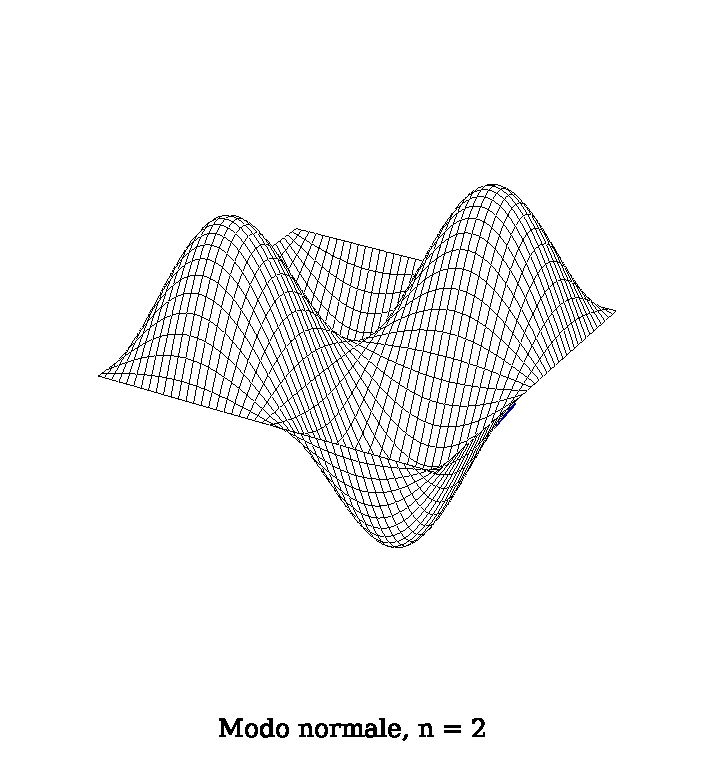
\includegraphics[width=0.5\linewidth]{modo_normale_singolo2.pdf}\hfill
    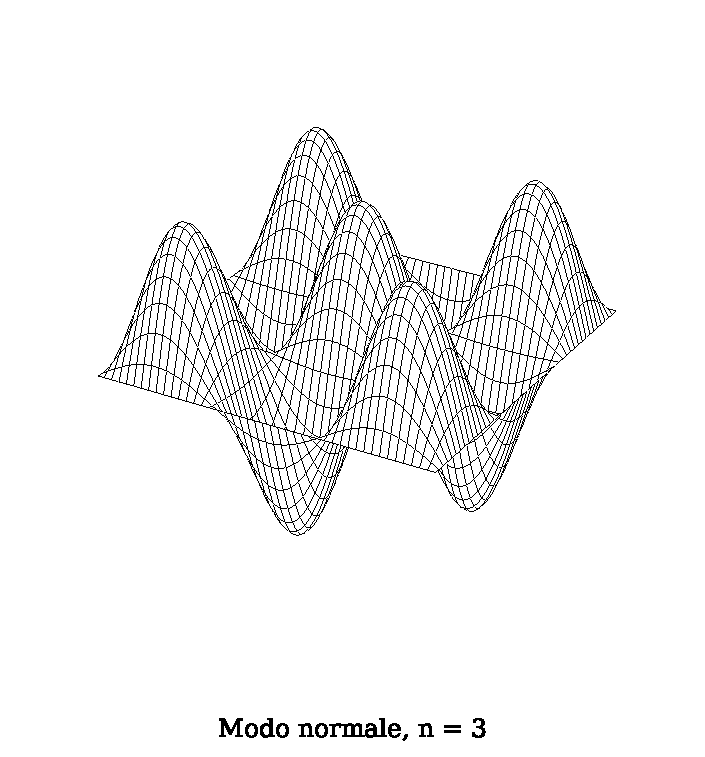
\includegraphics[width=0.5\linewidth]{modo_normale_singolo3.pdf}\hfill
\end{figure}
Le immagini evidenziano un aspetto strutturale preciso: ogni modo normale è una soluzione in cui la dipendenza spaziale e quella temporale sono completamente separate, ma rigidamente accoppiate nella forma del prodotto. La funzione spaziale $\sin(k_nx)$ determina la geometria della configurazione e, in particolare, la posizione dei nodi, che rimangono fissi per ogni istante temporale. La funzione temporale, invece, non modifica questa struttura, ma ne governa soltanto l’ampiezza globale attraverso un’oscillazione periodica (in questo caso, per maggiore uniformità, si ha a livello numerico $k_n=\omega_n$). All’aumentare di $n$, si osserva un incremento del numero di nodi interni: questo non corrisponde a una maggiore “dinamicità”, ma a una maggiore complessità della struttura spaziale imposta dalle condizioni al contorno. 
Ogni modo normale non descrive una propagazione della forma nello spazio, ma una oscillazione locale della configurazione stessa. In particolare, la cresta e i nodi della funzione spaziale restano fissi: non si spostano lungo il dominio, ma “vibrano” nel tempo mantenendo invariata la loro posizione. Ciò che varia è solo il valore della funzione in ciascun punto, che oscilla periodicamente, mentre la struttura complessiva del profilo rimane immobile.
In questo senso, le figure mostrano che la vera informazione della soluzione non è nella dinamica temporale, che è sempre regolare e prevedibile, ma nella struttura spaziale imposta dall’indice $n$. La complessità dell’evoluzione dell’equazione delle onde emerge solo quando questi modi vengono sovrapposti: il singolo modo, invece, rappresenta un’unità dinamica irriducibile.
\\
\\ \underline{\textbf{Curiosità}}: Il caso degli strumenti a corda è un esempio di equazione delle onde con condizione di Dirichlet, e i modi normali corrispondono agli armonici. Quindi, la prossima volta che avrete lezione di strumento, potrete stupire il vostro insegnante esponendogli la teoria sviluppata in questa sezione.

\newpage

\subsection{Regolarità e propagazione delle discontinuità}

Un aspetto delicato, che richiede di andare oltre l’ipotesi iniziale $\varphi\in C^2$, riguarda il comportamento delle possibili perdite di regolarità dei dati iniziali. In un contesto più generale, infatti, l’equazione delle onde non elimina tali irregolarità, ma ne governa la propagazione lungo le direzioni caratteristiche del sistema $(\eta,\xi)$.
\\
\\Consideriamo una funzione $\varphi(x,t)$ con una discontinuità nella derivata spaziale nel punto $x=x_0$. Abbiamo visto come il metodo di risoluzione di D'Alembert (\ref{sec: 4.2.1}) conduca a una soluzione della forma:
\[
\varphi(x,t)=f(x-vt)+g(x+vt)
\quad \Longrightarrow \quad
\partial_x \varphi(x,t)=f'(x-vt)+g'(x+vt)
\]

Ne segue che una possibile discontinuità della derivata si trasporta lungo le direzioni caratteristiche del problema. In particolare, essa si manifesta nei punti in cui gli argomenti delle derivate coincidono con la posizione iniziale della singolarità, cioè quando $x-vt=x_0$ oppure $x+vt=x_0$. Da ciò segue che la discontinuità si muove nello spazio-tempo secondo le leggi orarie:
\[
\begin{cases}
    x=x_0-vt \\
    x=x_0+vt
\end{cases}
\]

\subsubsection{\underline{Interpretazione grafica}}

Se prendiamo ad esempio una funzione che presenta una discontinuità della derivata nel punto $x=0$ all'istante $t=0$ come a esempio:
\[
\varphi(x,t)=\frac{1}{2}e^{-(x-vt)^2}\left(1-|x-vt|^\alpha\right)
+\frac{1}{2}e^{-(x+vt)^2}\left(1-|x+vt|^\alpha\right)\ \ , \ \ |\alpha|\lt 1
\]
Prese delle sezioni del grafico di $\varphi(x,t)$ a tempi fissati differenti ($t=0$, $t=0.5$, $t=1$):
\\
\\\begin{figure}[H]
    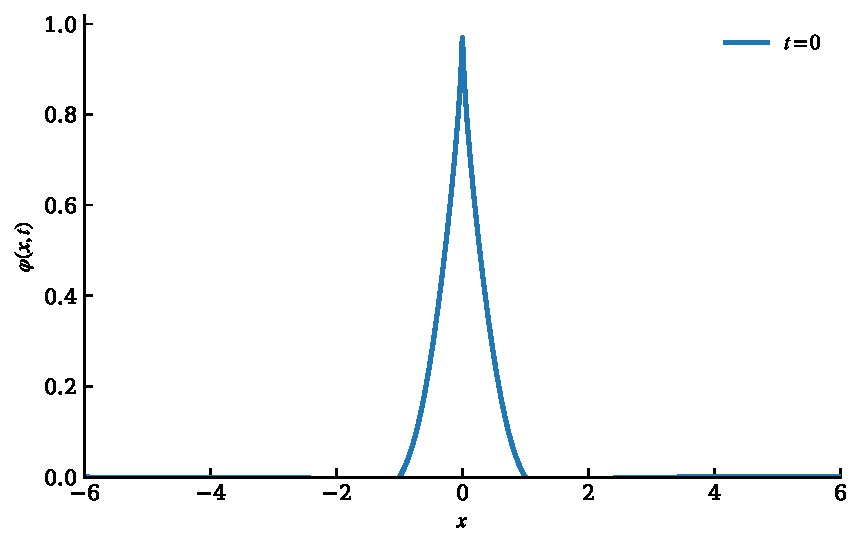
\includegraphics[width=0.33\linewidth]{cusp_wave_asymptote0.pdf}\hfill
    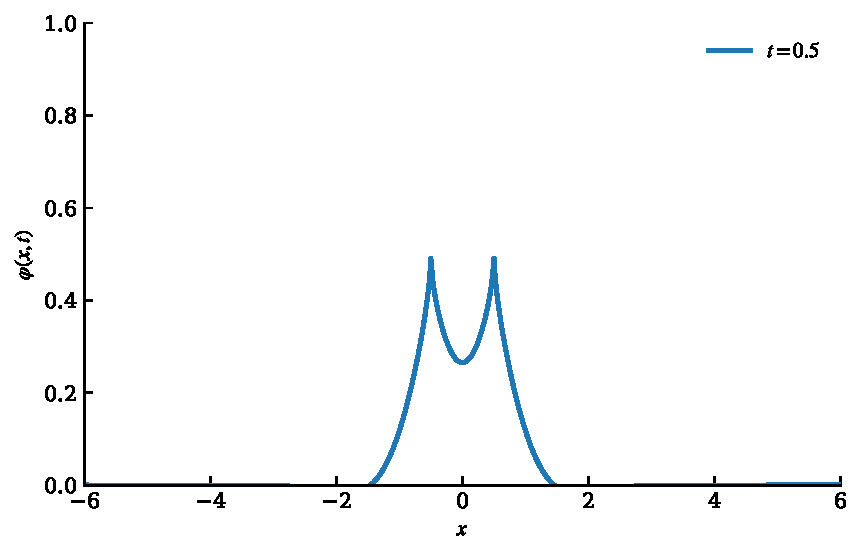
\includegraphics[width=0.33\linewidth]{cusp_wave_asymptote0.5.pdf}\hfill
    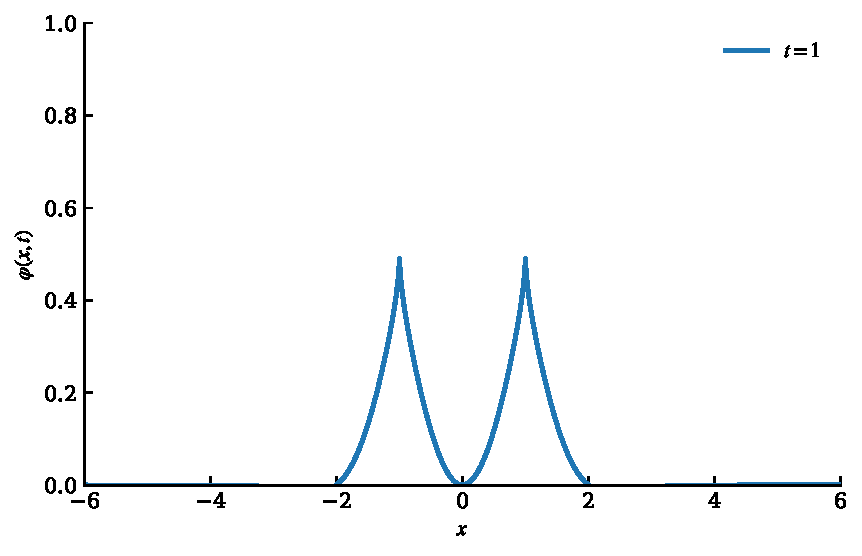
\includegraphics[width=0.33\linewidth]{cusp_wave_asymptote1.pdf}
\end{figure}
Notiamo come la discontinuità della derivata non venga in alcun modo attenuata o regolarizzata dall’evoluzione temporale. Al contrario, essa viene semplicemente trasportata lungo il dominio spaziale senza alterarne la natura. In particolare, le singolarità iniziali si muovono rigidamente secondo le leggi orarie precedentemente descritte, mantenendo invariata la loro struttura locale. Questo comportamento riflette la natura puramente iperbolica dell’equazione delle onde, in cui l’informazione non si diffonde ma si propaga lungo caratteristiche ben definite. Di conseguenza, la soluzione conserva memoria delle irregolarità iniziali, che persistono nel tempo come entità dinamiche.

\newpage

\section{Equazione di Laplace}

A differenza dell’equazione delle onde, che coinvolge una derivata seconda rispetto al tempo e descrive quindi una relazione di evoluzione, l’equazione di Laplace è composta esclusivamente da derivate spaziali di secondo ordine.

\begin{definizione}[Equazione di Laplace]
    Sia $\varphi(x,y): \Omega\subseteq \mathbb{R}^2\to \mathbb{R}$ una funzione sufficientemente regolare (in particolare $\varphi(x,y)\in C^2(\Omega)$. L'equazione di Laplace è una PDE di tipo ellittico (\ref{sec: 4.1.1}) della forma: $\displaystyle\pdd{\varphi}{x}+\pdd{\varphi}{y}=0$.
\end{definizione}

L’assenza di una variabile temporale implica che non esista una direzione privilegiata lungo cui il problema si può evolvere. Dal punto di vista matematico, questo si traduce nel fatto che non è possibile interpretare l’equazione come un problema di Cauchy ben posto nel tempo, ma piuttosto come una condizione di compatibilità spaziale globale. Infatti, la presenza esclusiva di derivate spaziali fa sì che il valore della soluzione in un punto non dipenda da una dinamica locale lungo una traiettoria, ma dall’interazione simultanea delle variazioni spaziali nelle direzioni coordinate. In altre parole, l’equazione impone che la curvatura complessiva del campo (somma delle curvature nelle direzioni ortogonali $(x,y)$) si annulli in ogni punto del dominio. Questa struttura spiega anche perché il problema non è determinato da dati iniziali, ma da condizioni al contorno: l’equazione non seleziona un’evoluzione a partire da un profilo iniziale, bensì ammette soluzioni che devono essere compatibili globalmente con vincoli imposti sui bordi del dominio.
\\Dal punto di vista fisico, questa stessa struttura si ritrova nei problemi di equilibrio, come nel caso del potenziale elettrostatico nel vuoto. In tali situazioni, l’assenza di sorgenti interne si traduce matematicamente nell’annullamento dell'equazione, e la configurazione del campo risulta completamente determinata dalla distribuzione ai bordi. Nei paragrafi successivi, analogamente al caso dell'equazione delle onde, vedremo come questa impostazione si traduca operativamente nella risoluzione del problema su domini semplici, e come la struttura dell’operatore conduca naturalmente a una descrizione in termini di modi spaziali e serie di Fourier. Ho inoltre dedicato un capitolo delle appendici all'analisi di alcuni casi di domini più esotici (\ref{app: cap 2}) compreso il caso di dominio sferico tridimensionale cui consiglio di dare un'occhiata soprattutto perchè mette in risalto diversi aspetti strutturali dell'equazione di Laplace, accompagnati anche da un'interpretazione grafica intuitiva.

\begin{definizione}[Operatore Laplaciano]\label{def: 4.12}
    Definiamo l'operatore differenziale Laplaciano nel modo seguente: $\Delta =:[\partial_x^2+\partial_y^2]$.
    \\
    \\Tipicamente può essere anche trovato (in contesti come quello dell'elettrostatica) espresso impropriamente tramite il simbolo di gradiente per $i\in\{1,...,n\}$ coordinate spaziali nel modo seguente: $\nabla^2=\displaystyle\sum_{i=1}^n\partial_{x_i}^2$.
\end{definizione}

Segue automaticamente che l'equazione di Laplace assume la seguente forma compatta:
\[\partial_x^2\varphi(x,y)+\partial_y^2\varphi(x,y)=0\iff \Delta\varphi(x,y)=0\]

\begin{proposizione}\label{prop: 4.3}
    L'equazione di Laplace è lineare nelle soluzioni.
    \\
    \\\underline{Dimostrazione}: Siano $\phi_1$ e $\phi_2$ soluzioni dell'equazione di Laplace e notiamo che una generica combinazione lineare $\lambda\phi_1+\mu\phi_2$ è soluzione.
    \\ Infatti: $\partial_x^2(\lambda\phi_1+\mu\phi_2)+\partial_x^2(\lambda\phi_1+\mu\phi_2)=\lambda\Delta\phi_1+\mu\Delta\phi_2=0$.\qed
\end{proposizione}


\newpage

\subsection{Dominio rettangolare}

Consideriamo adesso una funzione $\varphi(x,y)\in C^2$, consideriamo inoltre un dominio rettangolare $(x,y)\in [0,l_x]\times[0,l_y]$. Anche in questo caso definiamo delle condizioni di Dirichlet (\ref{def: 4.5}), quindi il problema che dobbiamo risolvere assume la forma seguente:
\[\begin{cases}
    \partial_x^2\varphi(x,y)+\partial_y^2\varphi(x,y)=0\iff \Delta\varphi(x,y)=0
    \\\varphi(x,0)=f_1(x)
    \\\varphi(x,l_y)=f_2(x)
    \\\varphi(0,y)=g_3(y)
    \\\varphi(l_x,y)=g_2(y)
\end{cases}\]
Notiamo che, così come è scritto, il problema risulta essere abbastanza ostico. Avvelendoci però del fatto che l'equazione di Laplace è lineare nelle soluzioni, possiamo costruire un problema equivalente ma molto più semplice da risolvere. Definiamo quindi:
\[\begin{cases}
    \Delta\phi^{(1)}=0
    \\\phi^{(1)}(x,0)=f_1(x)
    \\\phi^{(1)}(x,l_y)=0
    \\\phi^{(1)}(0,y)=0
    \\\phi^{(1)}(l_x,y)=0
\end{cases}\ \  \ \begin{cases}
    \Delta\phi^{(2)}=0
    \\\phi^{(2)}(x,0)=0
    \\\phi^{(2)}(x,l_y)=f_2(x)
    \\\phi^{(2)}(0,y)=0
    \\\phi^{(2)}(l_x,y)=0
\end{cases}\ \ \ \begin{cases}
    \Delta\phi^{(3)}=0
    \\\phi^{(3)}(x,0)=0
    \\\phi^{(3)}(x,l_y)=0
    \\\phi^{(3)}(0,y)=g_1(y)
    \\\phi^{(3)}(l_x,y)=0
\end{cases}\ \ \ \begin{cases}
    \Delta\phi^{(4)}=0
    \\\phi^{(4)}(x,0)=0
    \\\phi^{(4)}(x,l_y)=0
    \\\phi^{(4)}(0,y)=0
    \\\phi^{(4)}(l_x,y)=g_2(y)
\end{cases}\]
Notiamo ora che, grazie alla linearità dell’equazione di Laplace (\ref{prop: 4.3}), la somma di soluzioni è ancora una soluzione. Possiamo quindi decomporre il problema originario nella somma di quattro problemi più semplici, ciascuno caratterizzato da una sola condizione al bordo non omogenea. Infatti, se definiamo:
\[
\varphi(x,y)=\phi^{(1)}(x,y)+\phi^{(2)}(x,y)+\phi^{(3)}(x,y)+\phi^{(4)}(x,y),
\]
allora, per linearità dell’operatore laplaciano,
\[
\Delta\varphi
=
\Delta\phi^{(1)}
+
\Delta\phi^{(2)}
+
\Delta\phi^{(3)}
+
\Delta\phi^{(4)}
=
0.
\]
Inoltre, sommando le rispettive condizioni al bordo, si ricostruiscono esattamente le condizioni del problema iniziale. Ad esempio:
\[
\varphi(x,0)
=
\phi^{(1)}(x,0)
+
\phi^{(2)}(x,0)
+
\phi^{(3)}(x,0)
+
\phi^{(4)}(x,0)
=
f_1(x),
\]
poiché, per costruzione, soltanto \(\phi^{(1)}\) è non nulla su quel lato del bordo. Lo stesso ragionamento vale per tutti gli altri lati del rettangolo. Di conseguenza, invece di affrontare direttamente il problema completo, possiamo limitarci a risolvere un singolo problema elementare con una sola condizione al bordo non omogenea. La soluzione generale si ottiene poi per sovrapposizione lineare dei contributi corrispondenti ai quattro lati del dominio.
\\
\\ Concentriamoci quindi sulla risoluzione dell'equazione $\Delta\phi^{(1)}=0$ con le relative condizioni a contorno. Il primo passo è trovare una soluzione generale su tutto il dominio (quindi $\mathbb{R}^2$) e poi adattarlo alle condizioni a bordo.

\newpage

\subsubsection{\underline{Soluzione generale}}

Troviamo la soluzione generale (quindi senza alcun tipo di condizione) per la generica equazione di Laplace $\Delta\phi=0$. Per risolvere questo problema ci avvarremo della tecnica della separazione delle variabili già introdotta nella sezione dedicata all'equazione delle onde. Quindi supponiamo che esistano delle funzioni dipendenti rispettivamente dalle sole variabili $(x,y)$, $(X(x),Y(y))$ tali per cui la funzione $\phi(x,y)$ possa essere fattorizzata nel modo seguente: $\phi(x,y)=X(x)Y(y)$. Appicando l'operatore Laplaciano:
\[\Delta[\phi(x,y)]=\Delta[X(x)Y(y)]=Y(y)\partial_x^2X(x)+X(x)\partial_y^2Y(y)=Y(y)X''(x)+X(x)Y''(y)=0\]
Da cui ricaviamo $\displaystyle\frac{X''}{X}=-\frac{Y''}{Y}$ e deduciamo che l'unico modo per cui due espressioni in due variabili diverse siano uguali è che i contributi delle variabili $x$ e $y$ si annullino nelle frazioni. Definiamo quindi:
\[\begin{cases}
    \frac{X''}{X}=\lambda
    \\
    \\\frac{Y''}{Y}=-\lambda
\end{cases}\implies \begin{cases}
    X''-\lambda X=0
    \\ Y''+\lambda Y=0
\end{cases}\]
Per $\lambda=0$ la soluzione risulta banalmente lineare, mentre i casi realmente significativi sono quelli in cui $\lambda\neq0$. Osserviamo però una struttura sostanzialmente simmetrica del sistema: ponendo $\lambda=\omega^2\in \mathbb{R}$, si nota che, sia per $\lambda\gt 0$ sia per $\lambda\lt0$, le equazioni associate descrivono comunque una combinazione di un’oscillazione armonica e di un andamento esponenziale. Ciò che cambia non è quindi la natura qualitativa delle soluzioni, ma soltanto quale variabile assume il comportamento oscillatorio e quale quello esponenziale. Nel continuo si assume $\lambda\gt0$. Quindi:
\[\begin{cases}
    X''-\omega^2X=0\implies X(x)=A\sin(\omega x+\vartheta)
    \\Y''+\omega^2Y=0\implies Y(y)=B\sinh(\omega y+\gamma)
\end{cases}\]
Nel complesso, la separazione evidenzia una struttura in cui una direzione del dominio introduce oscillazioni, mentre l’altra impone una modulazione esponenziale, che verrà completamente determinata dalla geometria e dai vincoli del problema.

\subsubsection{\underline{Condizioni a contorno}}

Riprendiamo adesso le condizioni a contorno di Dirichlet definite nella pagina precedente e applichiamole alla soluzione generale trovata pocanzi:
\[\begin{cases}
    X(x)=A\sin(\omega x+\vartheta)
    \\\phi(l_x,y)=0\implies X(l_x)=0
    \\\phi(0,y)=0\implies X(0)=0
\end{cases}\implies \vartheta=0\ \ ,\ \ \omega=\omega_n=\frac{n\pi }{l_x}\ \ \text{con}\ \ n\in \mathbb{N}^+\]
Quindi abbiamo trovato una famiglia di soluzioni $X_n(x)=A_n\sin\bigg(\frac{n\pi x}{l_x}\bigg)$ con $n\in \mathbb{N}^+$. 
\\
\\ \underline{\textbf{Nota}}: Qui le $\omega$ non vanno intese come frequenze angolari nel senso fisico del termine (come si poteva fare nel caso delle onde); infatti si tratta solo di una notazione intuitiva per indicare il termine di pulsazione.

\newpage
Imponendo invece le condizioni di Dirichlet sul parametro dipendente da $y$ otteniamo:
\[\begin{cases}
    Y(y)=B\sinh(\omega y+\gamma)
    \\\phi(x,l_y)=0\implies Y(l_y)=0 
\end{cases}\implies Y(l_y)=B\sinh(\omega l_y+\gamma)=0\implies \gamma=-\omega l_y\]
Quindi, sostituendo $\omega=\omega_n=\displaystyle\frac{n\pi}{l_x}$, anche in questo caso ci ritroviamo con una famiglia di funzioni dipendenti da $n$: $Y_n(y)=B_n\sinh\bigg(\displaystyle\frac{n\pi}{l_x}(y-l_y)\bigg)$. Quindi la soluzione finale è una famiglia di soluzioni parametrizzate secondo $n\in\mathbb{N}^+$ della forma:
\[\phi_n(x,y)=X_n(x)Y_n(y)=A_nB_n\sin(\omega_nx)\sinh(\omega_n(y-l_y))=\alpha_n\sin\bigg(\frac{n\pi x}{l_x}\bigg)\sinh\bigg(\frac{n\pi}{l_x}(y-l_y)\bigg)\]
Nelle appendici è dimostrato come l'insieme dei seni costituisca una base completa dello spazio $L^2([0,l_x])$ (\ref{app: .7}), il che ci permette di esprimere una qualsiasi funzione di tale spazio mediante una serie di Fourier nella suddetta base. Quindi, seguendo un ragionamento perfettamente analogo a quello della sezione precedente (\ref{sec: 4.2.3}), possiamo scrivere la soluzione generale del problema come:
\[\phi(x,y)=\sum_{n=1}^\infty \alpha_n\sin\bigg(\frac{n\pi x}{l_x}\bigg)\sinh\bigg(\frac{n\pi}{l_x}(y-l_y)\bigg)\]
Manca ancora un ultimo passaggio. Infatti la soluzione, così come è definita, non è univoca poichè non viene specificato esplicitamente il parametro $\alpha_n$. Ebbene, per determinare quest'ultimo, è necessario applicare l'ultima condizione a contorno (e se vogliamo proprio quella più importante, poichè distingue il problema specifico di cui stiamo parlando dal caso omogeneo) ossia $\phi(x,0)=f_1(x)$. Essendo $f_1(x)\in L^2([0,l_x])$, è possibile esprimerlo in serie di Fourier nella base dei seni nel modo seguente: \[f_1(x)=\displaystyle\sum_{n=1}^\infty\xi_n\sin\bigg(\frac{n\pi x}{l_x}\bigg) \ \ ,\ \ \xi_n=\frac{2}{l_x}\int_0^{l_x}f_1(x)\sin\bigg(\frac{n\pi x}{l_x}\bigg)\,dx\implies\]
\[\phi(x,0)=f_1(x)\iff\sum_{n=1}^\infty\alpha_n\sin\bigg(\frac{n\pi x}{l_x}\bigg)\sinh\bigg(-\frac{n\pi l_y}{l_x}\bigg)=\sum_{n=1}^\infty\xi_n\sin\bigg(\frac{n\pi x}{l_x}\bigg)\]
Quindi deduciamo $\alpha_n=\xi_n\bigg[\sinh\bigg(-\displaystyle\frac{n\pi l_y}{l_x}\bigg)\bigg]^{-1}=-\xi_n\bigg[\sinh\bigg(\frac{n\pi l_y}{l_x}\bigg)\bigg]^{-1}$, abbiamo trovato
\\
\\quindi un'espressione univoca per $\phi^{(1)}(x,y)$. Quelle per $\phi ^{(i)}(x,y)$ si trovano in modo del tutto analogo. Quindi la soluzione generale del problema di Laplace con condizioni a contorno di Dirichlet su dominio rettangolare è:
\[\
    \varphi(x,y)=\sum_{j=1}^4\phi^{(j)}(x,y)=\sum_{j=1}^4\bigg[\sum_{n=1}^\infty\alpha_n^{(j)}\sin\bigg(\frac{n\pi x}{l_x}\bigg)\sinh\bigg(\frac{n\pi}{l_x}(y-l_y)\bigg)\bigg]\]

\noindent\textbf{Nota.} A questo punto qualcuno potrebbe domandarsi come si determinino gli \(\alpha_n\) associati alle condizioni al contorno dipendenti da \(y\), dato che non si tratta dello stesso spazio funzionale utilizzato per le condizioni in \(x\). In realtà il procedimento è del tutto analogo, ma va interpretato correttamente in termini di spazi \(L^2\) differenti. Anche le condizioni al contorno dipendenti da \(y\) possono essere sviluppate mediante serie di Fourier, ma lo spazio funzionale di riferimento non è lo stesso utilizzato per le condizioni dipendenti da \(x\). In particolare, mentre le funzioni \(f_1(x), f_2(x)\) appartengono naturalmente a \(L^2(0,l_x)\) e vengono espanse nella base trigonometrica su \([0,l_x]\), le funzioni \(g_1(y), g_2(y)\) appartengono a \(L^2(0,l_y)\) e devono quindi essere sviluppate nella corrispondente base su \([0,l_y]\). In questo senso, il metodo di separazione delle variabili induce due espansioni di Fourier distinte, ciascuna adattata al proprio dominio spaziale, senza che sia necessario (né coerente) utilizzare lo stesso spazio funzionale per entrambe le direzioni.
\\
\\Nel caso in cui i passaggi logici esposti non dovessero risultare chiari, si rimanda al paragrafo precedente, dove il metodo di separazione delle variabili è stato descritto in maniera molto più approfondita (\ref{sec: 4.2.3}).



\subsubsection{\underline{Interpretazione grafica}}

Per visualizzare concretamente la struttura delle soluzioni ottenute, riportiamo di seguito due esempi dei modi oscillatori $\phi_n(x,y)=\alpha_nX_n(x)Y_n(y)$ ai casi $n=2$ e $n=4$. 
\begin{figure}[H]
    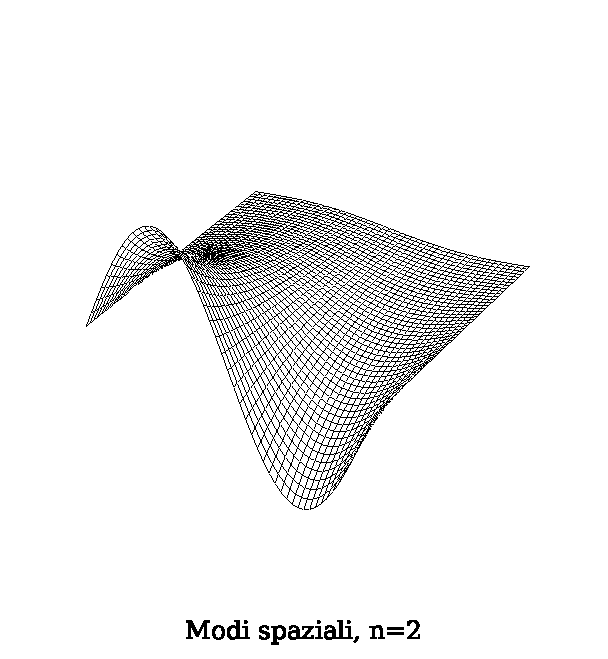
\includegraphics[width=0.5\linewidth]{laplace_modispaziali2.pdf}\hfill
    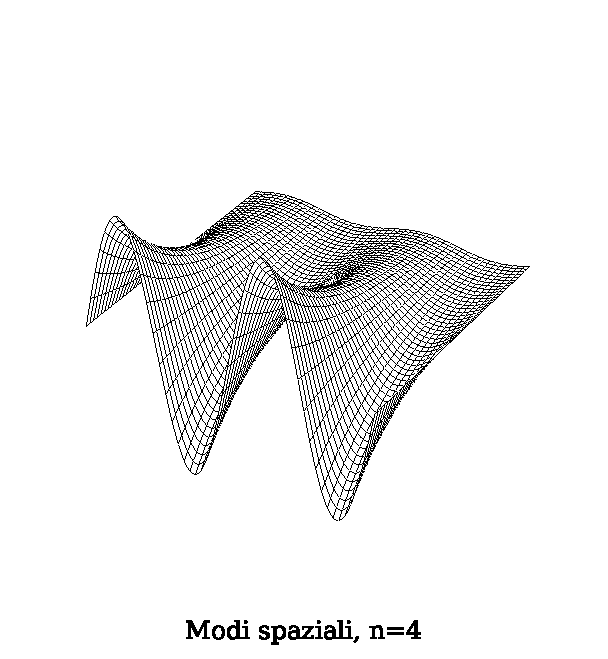
\includegraphics[width=0.5\linewidth]{laplace_modispaziali4.pdf}
\end{figure}

Notiamo anzitutto come all’aumentare di $n$, aumenti il numero di oscillazioni lungo la direzione $x$, mentre lungo $y$ la soluzione mantenga l’andamento esponenziale imposto dalla funzione $\sinh$. È importante distinguere questi modi dai modi normali dell’equazione delle onde. In quel caso le soluzioni descrivono oscillazioni dinamiche nel tempo; qui, invece, non essendo presente alcuna evoluzione temporale, i modi rappresentano semplicemente configurazioni spaziali statiche compatibili con le condizioni al bordo. Dal punto di vista fisico, questa struttura riflette il carattere di equilibrio tipico delle equazioni ellittiche. Un punto chiave è che questa configurazione non dipende da un processo di propagazione: ogni punto del dominio è determinato simultaneamente da tutti i valori al bordo. In altre parole, il bordo non agisce localmente ma influenza globalmente la soluzione, che si organizza in modo liscio e regolare proprio per minimizzare le variazioni interne compatibilmente con i vincoli esterni.

\newpage

\subsection{Dominio circolare}\label{sec: 4.3.2}

Adesso, continuando a sfruttare gli strumenti sviluppati nell’ambito della separazione delle variabili e dell’espansione in serie di Fourier dei modi di oscillazione, consideriamo nuovamente il problema di Dirichlet per l’equazione di Laplace. In questo caso il dominio scelto possiede simmetria circolare; risulta quindi naturale formulare il problema in coordinate polari. Lo studio di questa situazione costituisce il prototipo fondamentale per l’analisi delle equazioni ellittiche in geometrie radiali e permette di introdurre in modo naturale il nucleo di Poisson e la rappresentazione integrale delle funzioni armoniche nel disco. Consideriamo quindi un dominio $(r,\theta)\in[0,\mathcal{R}]\times[0,2\pi]$ e il problema:
\[\begin{cases}
    \Delta\varphi(r,\theta)=0
    \\
    \\\varphi(R,\theta)=f(\theta)
\end{cases}\]

\begin{proposizione}[Laplaciano in coordinate polari]\label{prop: 4.4}
    L'operatore Laplaciano (\ref{def: 4.12}), in coordinate polari $(r,\theta)$ assume la forma: $\Delta=\bigg[\displaystyle\pdd{}{r}+\frac{1}{r}\pd{}{r}+\frac{1}{r^2}\pdd{}{\theta}\bigg]$
    \\
    \\
    \\\underline{Dimostrazione}: In coordinate polari si ha la relazione $x=r\cos(\theta)$ e $y=r\sin(\theta)$, quindi derivando con la regola della derivazione a catena si ottiene:
    \[\begin{cases}
        \partial_x=\cos(\theta)\partial_r-\displaystyle\frac{\sin(\theta)}{r}\partial_\theta
        \\
        \\\partial_y=\sin(\theta)\partial_r+\frac{\cos(\theta)}{r}\partial_\theta
    \end{cases}\implies\begin{cases}
        \partial_x^2=\bigg(\cos(\theta)\partial_r-\displaystyle\frac{\sin(\theta)}{r}\partial_\theta\bigg)^2
        \\
        \\\partial_y^2=\bigg(\sin(\theta)\partial_r+\frac{\cos(\theta)}{r}\partial_\theta\bigg)^2
    \end{cases}\]
    \\
    \\Quindi, espandendo i conti si ottiene: \\
    \\\mbox{$\Delta=\partial_x^2+\partial_y^2=\bigg(\cos(\theta)\partial_r-\displaystyle\frac{\sin(\theta)}{r}\partial_\theta\bigg)^2+\bigg(\sin(\theta)\partial_r+\frac{\cos(\theta)}{r}\partial_\theta\bigg)^2=...=\partial_r^2+r^{-1}\partial_r+r^{-2}\partial_\theta^2$}\qed
\end{proposizione}
A seguito dei calcoli della proposizione precedente (che si fanno una sola volta nella vita), possiamo riscrivere l'equazione di Laplace in coordinate polari:
\[\Delta\varphi(r,\theta)=\pdd{\varphi}{r}+\frac{1}{r}\pd{\varphi}{r}+\frac{1}{r^2}\pdd{\varphi}{\theta}=0\]

Assumendo l'ipotesi di separazione delle variabili $\varphi(r,\theta)=R(r)\Theta (\theta)$, otteniamo:
\[\Delta\varphi(r,\theta)=\Theta(\theta)\partial_r^2R(r)+\frac{\Theta}{r}\partial_rR(r)+\frac{R(r)}{r^2}\partial_\theta^2\Theta(\theta)=\Theta R''+\Theta\frac{R'}{r}+\Theta''\frac{R}{r^2}=0\]
Riordinando algebricamente i termini otteniamo la seguente relazione: $r^2\displaystyle\frac{R''}{R}+r\frac{R'}{R}=-\frac{\Theta''}{\Theta}$

\newpage

Dato che l'uguaglianza precedente è posta tra funzioni di variabili differenti, deduciamo che siano costanti e definiamo le equazioni differenziali ordinarie:
\[\begin{cases}
    r^2R''+rR'=\lambda R
    \\\Theta''+\lambda\Theta=0
\end{cases}\]
Per avere maggiore ordine mentale, valutiamo tali equazioni separatamente.
\\
\\$\boxed{\text{Equazione angolare}}$  Valutiamo l'equazione $\Theta''=-\lambda\Theta$, ponendo $\lambda=\mu^2, \ \ \mu\in \mathbb{R}$. 
Dunque, le soluzioni generali assumono la forma $\Theta(\theta)=A\cos(\mu\theta)+B\sin(\mu\theta)$.
\\
\\Notiamo adesso che essendo $\theta\in (0,2\pi)$, la funzione $\Theta(\theta)$ deve essere periodica nell'intervallo di definizione della variabile (data la natura delle soluzioni trovate sopra). Questo accade solamente nel caso in cui $2\pi\mu=2\pi k$ con $k\in \mathbb{Z}$. Quindi possiamo riscrivere le soluzioni dell'equazione, sfruttando la notazione esponenziale, come 
\[\Theta_k(\theta)=C_ne^{ik\theta}\]
E notiamo che (a meno della costante $C_n$ che sarà assorbita dalla forma finale della soluzione più avanti) la famiglia $\Theta_k$ non ha valori in $L^2([0,2\pi])$, ma ne costituisce una base completa: la base degli esponenziali (\ref{app: .6}).
\\
\\$\boxed{\text{Equazione radiale}}$  Analizziamo adesso l'equazione radiale $r^2R''+rR'=\lambda R$. Dallo studio dell'equazione angolare abbiamo assunto $\lambda\in \mathbb{Z}$, per cui, anche in questo caso poniamo $\lambda=k^2\in \mathbb{Z}$. Un modo per risolvere l'equazione è assumere che $R(r)$ sia della forma $R(r)=r^\alpha,\ \ \alpha \in \mathbb{R}$. Quindi, sostituendo nell'equazione originale ci ritroviamo con:
\[r^2\alpha(\alpha-1)r^{\alpha-2}+r\alpha r^{\alpha-1}-k^2r=0\implies [\alpha(\alpha-1)+\alpha-k^2]r^\alpha=0\]
Poichè $r\in[0, \mathcal{R}]$, deduciamo che l'espressione sopra è nulla solamente quando il coefficiente tra parentesi quadre è nullo. Quindi:
\[\alpha(\alpha-1)+\alpha-k^2=0\implies\alpha=\pm|k|\implies R_k(r)=\zeta_kr^{|k|}+\xi_kr^{-|k|}\]
\underline{\textbf{Nota}}: Inserendo nell'equazione differenziale $k=0$, si ottiene $R_0(r)=\zeta_0+\xi_0\log r$. Lo si può mostrare per esercizio.

\subsubsection{\underline{Soluzione generale}}



\underline{\textbf{Nota}}: Nel problema di Dirichlet per l’equazione di Laplace nel disco $0\le r<R$, si richiede che la soluzione sia definita su tutto il dominio, incluso il punto $r=0$, che è interno al dominio stesso. Per garantire l’ammissibilità della soluzione si richiede almeno:
\[
\varphi \in C^2(\{r<R\}), 
\qquad 
\varphi \in L^\infty(B_\varepsilon(0)) \ \forall \varepsilon>0,
\]
cioè regolarità e limitatezza in un intorno dell’origine. Poiché $r^{-|k|}$ e $\log r$ divergono per $r\to 0$, tali contributi non appartengono allo spazio delle soluzioni ammissibili e si impone quindi $B_k=0 \quad \forall k$. In fisica una divergenza della soluzione in un punto interno del dominio rappresenterebbe quindi un comportamento non fisico del campo, equivalente all’introduzione di una concentrazione infinita non prevista dal modello.

\newpage

Per quanto detto nei paragrafi precedenti, le soluzioni generali dell'equazione possono essere espresse in un espansione in serie infinita indotta dalla serie di Fourier nella base degli esponenziali:
\[\varphi(r,\theta)=\sum_{k=-\infty}^\infty R_k(r)\Theta_k(\theta)=\sum_{k=-\infty}^\infty a_kr^{|k|}e^{ik\theta}\ \ \ \ ,  \ k\neq0
\]
Per determinare la successione $a_k$, naturalmente, è necessario applicare le condizioni a contorno.

\subsubsection{\underline{Condizioni a contorno}}

Imponendo le condizioni a contorno di Dirichlet $f(\theta)=\varphi(R,\theta)$ otteniamo la serie:
\[f(\theta)=\sum_{k=-\infty}^\infty a_nR^{|k|}e^{ik\theta}\]
E ci rendiamo subito conto che si tratta di una serie di Fourier espressa nella base degli esponenziali complessi (\ref{sec: 3.4.2}) (di cui conosciamo la definizione della costante). Imponiamo dunque l'uguaglianza tra la serie di Fourier complessa e il nostro risultato per determinare la costante $a_k$:
\[\sum_{k=-\infty}^\infty a_nR^{|k|}e^{ik\theta}=\sum_{k=-\infty}^\infty\bigg(\frac{1}{2\pi}\int_0^{2\pi}f(\tau)e^{-ik\tau}\,d\tau\bigg)e^{ik\theta}\implies a_n=\frac{R^{-|k|}}{2\pi}\int_0^{2\pi}f(\tau)e^{-ei\tau}\,d\tau\]
Quindi la soluzione generale dell'equazione di Laplace i coordinate polari con condizioni a contorno di Dirichlet assume la forma:
\[\varphi(r,\theta)=\sum_{k=-\infty}^\infty\frac{1}{2\pi}\bigg(\frac{r}R\bigg)^{|k|}\bigg(\int_0^{2\pi}f(\tau)e^{-ik\tau}\,d\tau\bigg)e^{ik\theta}=\int_0^{2\pi}\frac{\,d\tau}{2\pi}f(\tau)\sum_{k=-\infty}^\infty\bigg(\frac{r}{R}\bigg)^{|k|}e^{ik(\theta-\tau)} \]

\subsubsection{\underline{Nucleo di Poisson}}

E' possibile esprimere la soluzione appena trovata in forma integrale calcolando il valore della serie (la dimostrazione si può trovare nelle appendici (\ref{app: .7})):
\[\sum_{k=-\infty}^\infty\bigg(\frac{r}{R}\bigg)^{|k|}e^{ik(\theta-\tau)}=\frac{R^2-r^2}{R^2-2rR\cos(\theta-\tau)+r^2}=:P(r,\theta; R,\tau)\]
Dove $P(r,\theta; R,\tau)$ è detto nucleo di Poisson $\implies \varphi(r,\theta)=\displaystyle\frac{1}{2\pi}\int_0^{2\pi}f(\tau)P(r,\theta;R, \tau)\,d\tau$.
\\
\\Il nucleo di Poisson ha un ruolo concettualmente molto profondo nella teoria delle funzioni armoniche, perché non è soltanto uno strumento tecnico per risolvere il problema di Dirichlet nel disco, ma rappresenta in realtà un esempio canonico di kernel di approssimazione (\ref{def: 3.22}). L’idea fondamentale è che il valore della soluzione in un punto interno del dominio non viene assegnato localmente, ma si ricostruisce come combinazione dei valori assunti sul bordo, con pesi che dipendono dalla posizione del punto considerato. In particolare, la struttura del kernel fa sì che i contributi del bordo lontano vengano progressivamente attenuati rispetto a quelli più “vicini” in senso angolare.Quando il punto interno si avvicina alla frontiera, questa distribuzione di pesi si concentra sempre più in una regione ristretta del bordo, fino a diventare estremamente localizzata. Infatti per $\theta$ fissato
\[
\lim_{r\to R^-}P_r(\theta-\tau)=0,\ \ \lim_{r\to R^-}P_r(\theta-[\tau=\theta])=\lim_{r\to R^-}P_r(0)=\infty
\]
In termini più precisi, si tratta di una famiglia di funzioni regolari che converge (in senso distribuzionale) al comportamento della delta di Dirac (\ref{app: .13}), pur restando sempre una funzione liscia per ogni posizione interna. Questo fenomeno è del tutto analogo a quanto accade con i kernel che abbiamo analizzato nello studio delle serie di Fourier e dei teoremi di Weierstrass e Fejer, dove somme o medie parziali producono operatori di convoluzione che ricostruiscono progressivamente la funzione iniziale. Nel caso del nucleo di Poisson, però, questa struttura non deriva da un procedimento di troncamento o media di serie, ma emerge in modo intrinseco dalla soluzione del problema di Dirichlet per l’equazione di Laplace. In questa prospettiva, il nucleo di Poisson rende evidente un principio strutturale delle equazioni ellittiche: l’informazione non si propaga localmente lungo traiettorie, ma viene distribuita globalmente attraverso un meccanismo di media pesata. La soluzione in un punto interno non dipende da una porzione infinitesima del bordo, ma dall’intero dato al contorno, filtrato in modo geometrico dal kernel, che codifica esattamente quanto ciascuna porzione della frontiera contribuisce al valore interno.

\subsubsection{\underline{Interpretazione grafica}}

Di seguito sono riportati due immagini di modi normali in coordinate polari. L'interpretazione è del tutto analoga a quella dei modi in coordinate cartesiane; cambia solamente la forma.

\begin{figure}[H]
    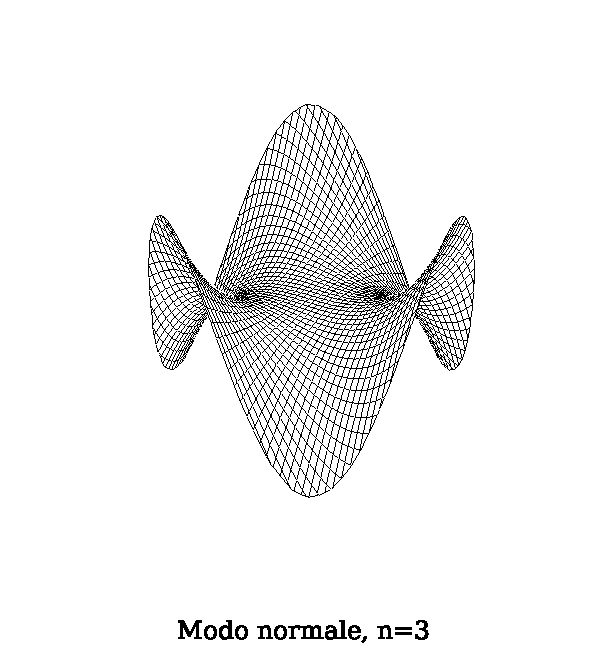
\includegraphics[width=0.5\linewidth]{laplace_modispazialidisco3.pdf}\hfill
   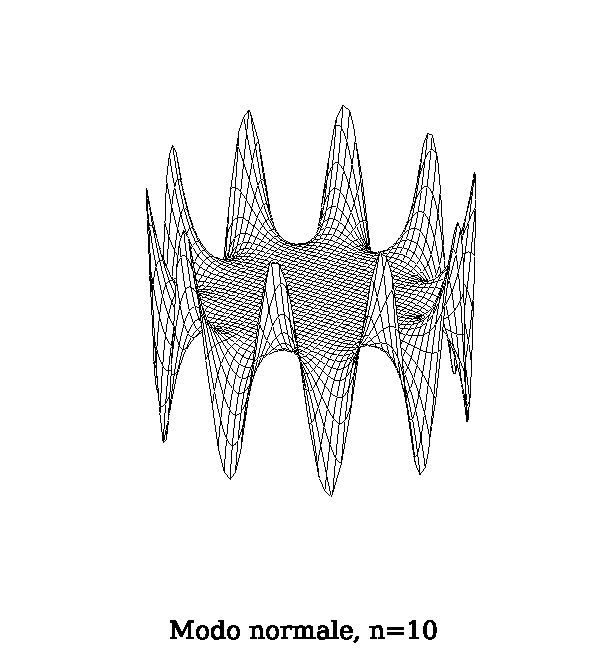
\includegraphics[width=0.5\linewidth]{laplace_modispazialidisco10.pdf}
\end{figure}
\underline{\textbf{Nota}}: Il plot è stato realizzato utilizzando la rappresentazione reale dei modi armonici, in particolare tramite il termine coseno, che consente una visualizzazione diretta delle strutture nodali nel disco. La formulazione complessa tramite gli $e^{ik\theta}$ contiene invece simultaneamente le informazioni associate alle componenti reale e immaginaria, corrispondenti rispettivamente ai contributi sinusoidale e cosinusoidale della soluzione.

\newpage

\subsection{Regolarità}\label{sec: 4.3.3}

Per chiudere il quadro, vale la pena soffermarsi sulla natura delle soluzioni ottenute, studiandone in particolare regolarità e convergenza. A differenza di altri problemi differenziali, l’equazione di Laplace possiede un forte effetto regolarizzante: anche dati al bordo poco regolari generano soluzioni immediatamente lisce all’interno del dominio. Per mostrare questo fatto, partiamo dalla soluzione generale del problema di Laplace con condizioni di Dirichlet: 
\[
\varphi(x,y)=\sum_{n=1}^\infty A_n\sin\bigg(\frac{n\pi x}{l_x}\bigg) \ \ ,\ \ A_n=\xi_n \sinh\bigg(\frac{n\pi}{l_x}(l_y-y)\bigg)\bigg[\sinh\bigg(\frac{n\pi l_y}{l_x}\bigg)\bigg]^{-1}
\]
Dove $\xi_n$ è il coefficiente di Fourier nella base dei seni. Possiamo fare una stima del coefficiente $A_n$ della soluzione utilizzando il lemma (\ref{app: .5}), ottenendo la seguente relazione tramite applicazione diretta:
Si ottiene
\[
\left|
\frac{
\sinh\!\left(\frac{n\pi}{l_x}(l_y-y)\right)
}{
\sinh\!\left(\frac{n\pi}{l_x}l_y\right)
}
\right|
\le
\frac{
e^{-\frac{n\pi}{l_x}y}
}{
1-e^{-\frac{2n\pi}{l_x}l_y}
}\implies 
|A_n(y)|
\le
|\xi_n|
\frac{
e^{-\frac{n\pi}{l_x}y}
}{
1-e^{-\frac{2n\pi}{l_x}l_y}
}
\le
C_y\,|\xi_n|\,e^{-\frac{n\pi}{l_x}y}
\]
Con $C_y=:\displaystyle\frac{1}{1-e^{-\frac{2\pi l_x}{l_y}}}$. Segue quindi che i coefficienti della soluzione dell'equazione di Laplace sono governati da un decadimento esponenziale rispetto all'indice $n$ della serie.

\begin{teorema}[Regolarità interna delle soluzioni di Laplace]
Sia $\varphi(x,y)$ soluzione del problema di Laplace su
$\Omega=[0,l_x]\times[0,l_y]$, con condizione al bordo di Dirichlet
$f(x)=\varphi(x,0)$ tale che $f\in L^2([0,l_x])$.
Siano $\xi_n$ i coefficienti di Fourier di $f$ nella base dei seni.
Allora la soluzione ottenuta tramite separazione delle variabili soddisfa
\[
\varphi \in C^\infty\big([0,l_x]\times[y_0,l_y]\big)
\qquad \forall\, y_0>0.
\]
\underline{Dimostrazione}: Scriviamo la soluzione nella forma $\varphi(x,y)=\sum_{n=1}^{\infty}
A_n(y)\sin\!\left(\frac{n\pi x}{l_x}\right)$, con stima $|A_n(y)| \le C_y |\xi_n| e^{-\frac{n\pi}{l_x}y}$ dimostrata sopra. Se fissiamo \(y_0>0\), si ha in particolare
\[
|A_n(y)| \le C_{y_0} |\xi_n| e^{-c n y_0},
\qquad c=\frac{\pi}{l_x}.
\]
Derivando termine a termine, ogni derivata \(\partial_x^k\partial_y^h\)
introduce al più un fattore polinomiale \(n^{k+h}\), quindi:
\[
\left|
\partial_x^k \partial_y^h
\Big(
A_n(y)\sin\!\left(\frac{n\pi x}{l_x}\right)
\Big)
\right|
\le
C_{k,h,y_0}\,
n^{k+h}\,
|\xi_n|\,
e^{-c n y_0}\implies
\left|\partial_x^k\partial_y^h \varphi(x,y)\right|
\le
\sum_{n=1}^{\infty}
n^{k+h}|\xi_n|e^{-c n y_0}
\]
Poiché \((\xi_n)\in \ell^2\) (\ref{sec: 2.2.5}) e il fattore esponenziale domina qualunque crescita polinomiale in \(n\), la serie converge assolutamente e uniformemente su ogni insieme del tipo \(y\ge y_0>0\). Ne segue che è lecito derivare termine a termine la serie infinite volte, e quindi tutte le derivate sono continue. Pertanto $\varphi \in C^\infty\big([0,l_x]\times[y_0,l_y]\big).
\qquad $ \qed

\end{teorema}

\newpage

Il teorema mostra una proprietà strutturale fondamentale dell’equazione di Laplace: la soluzione diventa automaticamente liscia all’interno del dominio anche quando il dato al bordo è soltanto quadrato-integrabile. Questo effetto di regolarizzazione è una delle differenze più profonde rispetto alle equazioni evolutive di tipo iperbolico. L’introduzione di \(y_0>0\) è essenziale perché separa il bordo, dove la regolarità può essere persa, dall’interno del dominio: appena ci si allontana dal bordo, le componenti ad alta frequenza vengono smorzate esponenzialmente e la soluzione acquista derivabilità infinita. In altre parole, \(y_0\) serve a garantire un controllo uniforme che non sarebbe possibile includendo il bordo stesso. Questo comportamento contrasta nettamente con l’equazione delle onde: nel caso iperbolico le discontinuità e le irregolarità del dato iniziale si propagano lungo le caratteristiche senza essere smorzate, mantenendo nel tempo la stessa “rugosità” iniziale. Per Laplace invece non esiste propagazione nel senso dinamico, ma una mediazione globale che elimina progressivamente le oscillazioni ad alta frequenza. Ne risulta che, mentre l’equazione delle onde conserva la struttura fine del dato, l’equazione di Laplace la “dissolve” immediatamente nell’interno del dominio.
\\
\\Per concludere lo studio della soluzione del problema di Dirichlet per l’equazione di Laplace, è importante chiarire in che senso la soluzione ricostruisce il dato al bordo. In particolare, si verifica che la convergenza verso la funzione assegnata avviene nel senso della norma $L^2$, che è il contesto naturale per dati non necessariamente regolari.

\begin{teorema}[Convergenza in $L^2$]
    Sia $\varphi(x,y)$ la soluzione del problema di Laplace su $\Omega=[0,l_x]\times[0,l_y]$, con condizione a contorno di Dirichlet $f(x)=\varphi(x,0)\in L^2(0,l_x)$ e coefficienti di Fourier $\xi_n$.
    \\Allora vale la convergenza in norma $L^2$, quindi: $\lim_{y\to 0^+}\|\varphi(x,y)-f(x)\|_{L^2(0,l_x)}$.
    \\
    \\\underline{Dimostrazione}: Fissato $y\gt 0$, e posto $\alpha_n(y)=:\sinh\bigg(\displaystyle\frac{n\pi}{l_x}(l_y-y)\bigg)\bigg[\sinh\bigg(\frac{n\pi}{l_x}l_y\bigg)\bigg]^{-1}$, possiamo scrivere la soluzione del problema di Laplace come: $\varphi(x,y)=\displaystyle\sum_{n=1 }^\infty \xi_n\alpha_n\sin\bigg(\frac{n\pi x}{l_x}\bigg)$.
    \\
    \\Sviluppando $f(x)$ abbiamo: $\|\varphi(x,y)-f(x)\|^2_{L^2([0,l_x])}=\displaystyle\int_0^{l_x}\bigg|\sum_{n=1}^\infty \xi_n(\alpha_n-1)\sin\bigg(\frac{n\pi x}{l_x}\bigg)\bigg|^2\,dx$
    \\ 
    \\Poniamo adesso $a_n=:\xi_n(\alpha_n-1)$; sviluppando il quadrato otteniamo:
    \\
    \\$=\displaystyle\int_0^{l_x}\sum_{n=1}^\infty\sum_{m=1}^\infty a_na_m\sin\bigg(\frac{n\pi x}{l_x}\bigg)\sin\bigg(\frac{m\pi x}{l_x}\bigg)\,dx=\sum_{n=1}^\infty\sum_{m=1}^\infty a_na_m\int_0^{l_x}\sin\bigg(\frac{n\pi x}{l_x}\bigg)\sin\bigg(\frac{m\pi x}{l_x}\bigg)\,dx$
    \\
    \\
    \\$\displaystyle=\sum_{n=1}^\infty\sum_{m=1}^\infty a_na_m\frac{l_x}{2}\delta_{mn}=\sum_{n=1}^\infty a_n^2\frac{l_x}{2}=\sum_{n=1}^\infty(\xi_n(\alpha_n-1))^2\frac{l_x}{2}$. 
    \\
    \\
    \\Notiamo ora che, poichè $\xi_n\in \ell^2$, è quadrato sommabile per definizione (ossia la serie dei suoi quadrati converge); inolte $\lim_{y\to 0^+}\alpha_n=1$. \\Quindi $\displaystyle\lim_{y\to 0^+}\|\varphi(x,y)-f(x)\|^2_{L^2}=\lim_{y\to 0^+}\frac{l_x}{2}\sum_{n=1}^\infty\xi_n^2(\alpha_n-1)^2=0$. \qed

\end{teorema}

\newpage

\section{Equazione del calore}

Per concludere il capitolo, è utile introdurre brevemente un esempio di equazione parabolica: l’equazione del calore. Essa rappresenta il prototipo dei problemi di diffusione; infatti descrive l’evoluzione nel tempo di una quantità fisica (come la temperatura) sottoposta a un processo di dissipazione, ed è caratterizzata da un comportamento profondamente diverso rispetto alle equazioni di tipo iperbolico ed ellittico già studiate. Sebbene questo argomento non sia stato trattato in dettaglio durante le lezioni, si consiglia comunque una breve lettura delle sue idee fondamentali, in quanto permette di completare il quadro concettuale sulle equazioni differenziali e sulle loro proprietà qualitative.

\begin{definizione}[Equazione del calore]
    Sia $\varphi:(0,L)\times(0,T)\to \mathbb{R}$. Definiamo equazione del calore o equazione di Fourier la PDE della forma: $\displaystyle\pd{\varphi}{t}-C\pdd{\varphi}{x}=0$.
\end{definizione}

l’equazione è detta parabolica perché la parte principale (quella delle derivate seconde) ha una sola direzione spaziale e non ammette propagazione bidirezionale come nel caso iperbolico. In termini del simbolo principale, il termine $\partial_x^2$ è di tipo ellittico mentre l’evoluzione nel tempo $\partial_t$ introduce una direzionalità privilegiata che rompe la simmetria temporale. Questa combinazione produce un comportamento diffusivo, tipico delle equazioni paraboliche.

\subsubsection{\underline{Soluzione}}

Per determinare una soluzione esatta dell'equazione ci serviremo della tecnica della separazione delle variabili e seguiremo lo stesso procedimento risolutivo applicato durante tutto il capitolo. Consideriamo quindi l'equazione del calore con condizioni iniziali e condizioni a contorno di Dirichlet:
\[\begin{cases}
    \partial_t\varphi(x,t)-C\partial_x^2\varphi(x,t)=0
    \\\varphi_0=\varphi(x,0)=f(x)
    \\\varphi(0,t)=\varphi(L,t)=0
\end{cases}\]
Assumendo la separazione delle variabili otteniamo le seguenti equazioni differenziali ordinarie: 
\[\varphi(x,t)=X(x)T(t)\implies X(x)T'(t)-CT(t)X''(x)=0\implies\begin{cases}
    X''+\lambda X=0
    \\T'+\lambda CT=0
\end{cases}\]
Abbiamo già ricavato l'espressione in termini di serie di Fourier della soluzione dell'equazione spaziale che (date le condizioni a contorno) impone soluzioni discrete del tipo
\[X_n(x)=A_n\sin\bigg(\frac{n\pi x}{L}\bigg)\]
L'equazione temporale invece implica una semplice soluzione esponenziale. Includendo i risultati di discretizzazione imposti dall'equazione spaziale otteniamo:
\[T_n(t)=B_n e^{-C\frac{n\pi t}{L}}\]
Quindi, inglobando le costanti in un'unica costante $\alpha_n$, la soluzione generale espressa 

\newpage

tramite le serie di Fourier assume la forma seguente: $\varphi(x,t)=\displaystyle\sum_{n=1}^\infty\alpha_n\sin\bigg(\frac{n\pi x}{L}\bigg) e^{-C\frac{n\pi t}{L}}$.
Per trovare la soluzione particolare (quindi la forma univoca del coefficiente n-esimo $\alpha_n$), confrontiamo la soluzione trovata calcolata in $t=0$ con l'espansione in serie di Fourier del termine $\varphi_0\in L^2([0,L])$:
\[\varphi(x,0)=\sum_{n=1}^\infty\alpha_n\sin\bigg(\frac{n\pi x}{L}\bigg)=\sum_{n=1}^\infty s_n\sin\bigg(\frac{n\pi x}{L}\bigg)=f(x) \ \ , \ \ s_n=\frac{2}{L}\int_0^Lf(s)\sin\bigg(\frac{n\pi s}{L}\bigg)\,ds\]
Concludiamo quindi che $\alpha_n=s_n$, e quindi la soluzione finale dell'equazione del calore con condizioni di Dirichlet assume la forma seguente:
\[\varphi(x,t)=\frac{2}{L}\sum_{n=1}^\infty\bigg(\int_0^Lf(s)\sin\bigg(\frac{n\pi s}{L}\bigg)\,ds\bigg)\sin\bigg(\frac{n\pi x}{L}\bigg)e^{-C\frac{n\pi t }{L}}\]
La struttura della soluzione mette in evidenza una proprietà fondamentale dell’equazione del calore: l’evoluzione temporale agisce come un meccanismo di dissipazione delle componenti oscillanti del dato iniziale. Ogni termine della serie
\[
\sin\!\left(\frac{n\pi x}{L}\right)e^{-C\left(\frac{n\pi}{L}\right)^2 t}
\]
rappresenta un modo spaziale indipendente, caratterizzato da una frequenza \(n\). La parte sinusoidale descrive la distribuzione spaziale della temperatura, mentre il fattore esponenziale governa il decadimento temporale del modo. L’aspetto cruciale è la presenza del termine quadratico \(n^2\) nell’esponente: i modi ad alta frequenza decadono molto più rapidamente di quelli a bassa frequenza. Dal punto di vista fisico, questo significa che le variazioni molto brusche della temperatura vengono eliminate quasi immediatamente, mentre le strutture più ampie persistono più a lungo. 
Questo comportamento riflette la natura diffusiva del fenomeno termico: in un materiale conduttore, il calore tende spontaneamente a redistribuirsi dalle regioni più calde a quelle più fredde, riducendo i gradienti di temperatura. La soluzione matematica mostra precisamente questo processo: il sistema perde progressivamente memoria dei dettagli fini del dato iniziale e converge verso configurazioni sempre più uniformi.
Dal punto di vista analitico, il decadimento esponenziale implica inoltre una forte regolarizzazione della soluzione, similmente a quanto accade per Laplace. Anche se il dato iniziale \(f(x)\) fosse soltanto in \(L^2\), per ogni \(t>0\) la soluzione diventa automaticamente \(C^\infty\) (la dimostrazione segue gli stessi passaggi logici della (\ref{sec: 4.3.3})). Questo distingue profondamente l’equazione del calore da quella delle onde: mentre le equazioni iperboliche propagano le irregolarità lungo le caratteristiche, l’equazione del calore le smorza istantaneamente.
\\
\\A differenza dell’equazione di Laplace, che descrive configurazioni stazionarie determinate interamente dai dati al bordo, l’equazione del calore introduce una vera evoluzione temporale. Le soluzioni dell’equazione di Laplace rappresentano stati di equilibrio già raggiunti, mentre l’equazione del calore descrive il processo dinamico attraverso cui il sistema evolve verso tale equilibrio. Dal punto di vista analitico, entrambe le equazioni possiedono proprietà regolarizzanti, ma nel caso del calore la regolarizzazione è accompagnata da un decadimento temporale dei modi spaziali: le componenti ad alta frequenza vengono smorzate esponenzialmente nel tempo, riflettendo il carattere dissipativo del fenomeno diffusivo.

\newpage

\subsubsection{\underline{Interpretazione grafica}}

Le figure seguenti mostrano alcune approssimazioni troncate della soluzione dell’equazione del calore ottenute mantenendo soltanto un numero finito di modi normali nella serie di Fourier. Ogni grafico rappresenta quindi la sovrapposizione dei primi n modi spaziali, ciascuno evoluto temporalmente secondo il proprio fattore di decadimento esponenziale.
\begin{figure}[H]
    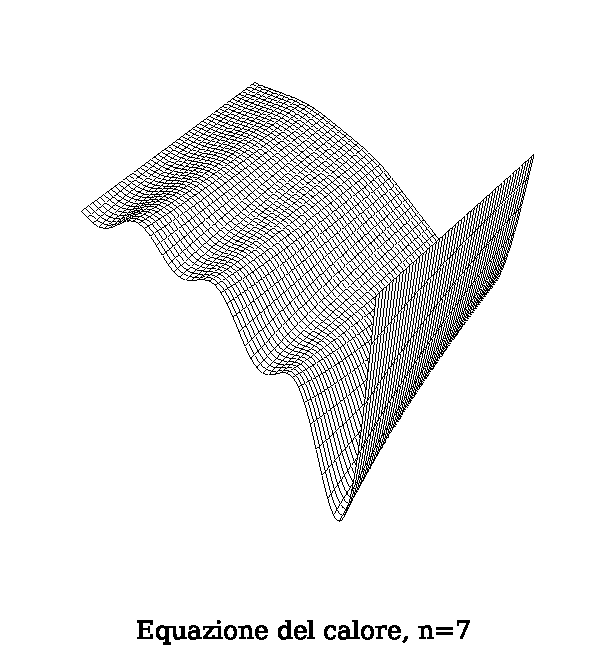
\includegraphics[width=0.5\linewidth]{equazionecalore7.pdf}\hfill
    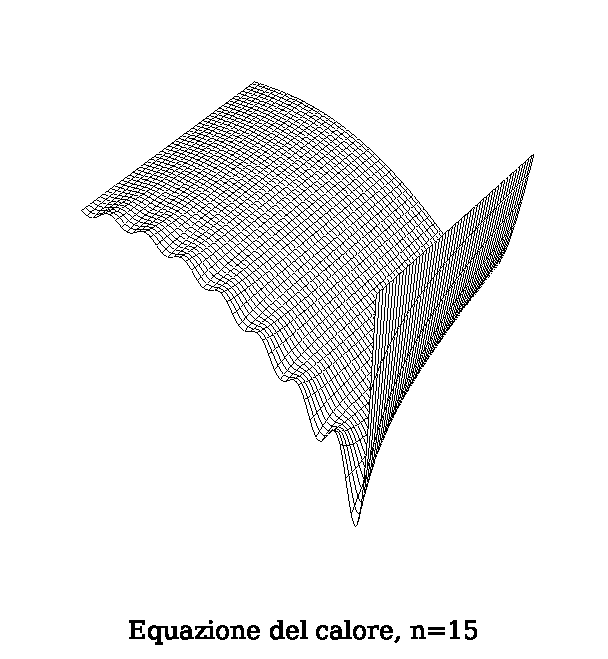
\includegraphics[width=0.5\linewidth]{equazionecalore15.pdf}
\end{figure}
Anche se nei grafici non si osservano i singoli modi separatamente, ma la loro somma complessiva, l’effetto della dinamica resta chiaramente visibile nella forma globale della soluzione. Infatti ogni contributo della serie è moltiplicato dal fattore$e^{-C\left(\frac{n\pi}{L}\right)^2 t}$, che dipende quadraticamente dalla frequenza \(n\). Questo implica che, al crescere del tempo, i termini con \(n\) grande diventano rapidamente trascurabili nella somma totale. Di conseguenza, le oscillazioni più fini della soluzione (generate proprio dai modi ad alta frequenza) scompaiono progressivamente, lasciando dominare soltanto le componenti più lente e regolari.
Dal punto di vista matematico, la soluzione evolve quindi verso configurazioni sempre più lisce perché la serie perde gradualmente i contributi responsabili delle variazioni rapide nello spazio. La dissipazione non agisce direttamente sulla forma finale della somma, ma sui coefficienti temporali dei singoli modi che la compongono.

\newpage

\chapter{\ Teoria degli operatori}
\vspace{2cm}
La teoria degli operatori rappresenta probabilmente la parte più astratta dell’intero corso di Metodi 1. Nei capitoli precedenti abbiamo introdotto numerosi strumenti dell’analisi funzionale (spazi normati, spazi di Hilbert, serie di Fourier, spazi $L^p$) spesso lavorando con oggetti concreti come successioni, funzioni o soluzioni di equazioni differenziali. In questo capitolo compiremo invece un ulteriore passo verso un livello di astrazione maggiore: non studieremo più solamente gli elementi di uno spazio funzionale, ma le trasformazioni che agiscono su di essi.
L’idea centrale è quella di generalizzare il concetto di matrice e di applicazione lineare dal caso finito-dimensionale a contesti infinito-dimensionali. In dimensione finita molti aspetti dell’algebra lineare risultano quasi automatici: ogni applicazione lineare continua è rappresentabile tramite una matrice, gli autovalori si ottengono tramite il polinomio caratteristico e, in molti casi, gli operatori possono essere diagonalizzati scegliendo opportunamente una base. Negli spazi di Hilbert infinito-dimensionali la situazione diventa notevolmente più delicata e ricca di fenomeni nuovi.
Compariranno infatti concetti che non hanno un vero analogo semplice in dimensione finita, come lo spettro continuo, gli operatori compatti o le diverse nozioni di convergenza operatoriale. Molti risultati familiari dell’algebra lineare continueranno a valere solo sotto ipotesi aggiuntive, mentre altri dovranno essere riformulati in modo più generale. Proprio per questo motivo la teoria degli operatori costituisce uno dei punti di incontro più importanti tra algebra lineare, analisi funzionale e fisica matematica.
Dal punto di vista fisico, gli operatori svolgono un ruolo fondamentale in quasi tutti gli ambiti della fisica teorica moderna. In meccanica quantistica, ad esempio, le osservabili fisiche vengono descritte tramite operatori autoaggiunti su spazi di Hilbert e le simmetrie del sistema sono rappresentate da operatori unitari. Anche le serie di Fourier, introdotte nei capitoli precedenti, possono essere comprese più profondamente attraverso il linguaggio operatoriale e il teorema spettrale.
Nonostante il livello di astrazione possa inizialmente apparire elevato, molti dei concetti introdotti in questo capitolo possono essere interpretati come generalizzazioni naturali di idee già note dall’algebra lineare elementare. Per questo motivo sarà utile mantenere costantemente il parallelismo tra matrici finite-dimensionali e operatori su spazi di Hilbert: gran parte dell’intuizione geometrica sviluppata nel caso finito continuerà infatti a rimanere valida, pur richiedendo strumenti analitici più sofisticati.
L’obiettivo finale del capitolo sarà quello di comprendere come certe classi di operatori possano essere “diagonalizzate” anche in dimensione infinita attraverso il teorema spettrale, uno dei risultati più importanti dell’analisi funzionale.

\newpage

\section{Operatori lineari continui}

Una volta introdotti gli spazi normati e gli spazi di Hilbert, possiamo studiare le applicazioni lineari che agiscono su tali strutture preservandone le proprietà algebriche e topologiche. In dimensione infinita, a differenza di quanto accade nel caso matriciale finito-dimensionale, non tutte le applicazioni lineari hanno un comportamento regolare: la continuità diventa quindi una proprietà fondamentale. Gli operatori lineari continui costituiscono la classe di trasformazioni più importante dell’analisi funzionale. Essi permettono infatti di estendere molti risultati dell’algebra lineare classica a contesti infinito-dimensionali, mantenendo un buon controllo sul comportamento di successioni, limiti e convergenze. In questa sezione introdurremo le definizioni fondamentali di operatore lineare, continuità e norma operatore, discutendo inoltre alcuni esempi significativi che compariranno frequentemente nel seguito.



\begin{definizione}[Operatore lineare]
    Siano $V$ e $W$ due spazi vettoriali sullo stesso campo $\mathbb{K}$ (considereremo prevalentemente i campi $\mathbb{R}$ o $\mathbb{C}$). Una mappa $T:\delta_T\subseteq V\to W$ è un operatore  lineare se: 
    \[T(\lambda v +\mu w)=\lambda T(v)+\mu T(w) \ \ \forall \lambda, \mu \in \mathbb{K}\ \  \forall v, w\in V\]
\end{definizione}
Dalla definizione si ricava facilmente che $T(0)=0$ e che $T(-v)=-T(v)$ perchè:
\[T(0)=T(0+0)=2T(0)\iff T(0)=0\]
\[T(-v)=T(-1(v))=-T(v)\]
È importante osservare che, in generale, un operatore non è necessariamente definito su tutto lo spazio vettoriale di riferimento. Per questo motivo, spesso si introduce esplicitamente il dominio dell’operatore. Più precisamente, un operatore lineare viene indicato nella forma
\[T:\delta_T\subseteq V\to Im(T)\subseteq W\]
Questa distinzione risulta particolarmente importante nello studio degli operatori differenziali e, più in generale, degli operatori non limitati, nei quali non è quasi mai possibile definire l’operatore su tutto lo spazio funzionale considerato.
In molti casi sarà comunque possibile estendere opportunamente il dominio dell’operatore oppure costruire estensioni dell’operatore stesso con proprietà più regolari.

\subsection{Continuità e limitatezza}

Una delle proprietà più importanti degli operatori lineari tra spazi normati riguarda la stretta relazione tra continuità e limitatezza. A differenza di quanto accade per funzioni generiche, nel caso lineare il comportamento dell’operatore risulta completamente determinato dal suo comportamento in un singolo punto, l’origine.
Il prossimo teorema che analizzeremo ci fornirà infatti diverse caratterizzazioni equivalenti della continuità di un operatore lineare. In particolare, esso mostra che richiedere la continuità dell'operatore lineare $T$ equivale a imporre una stima del tipo
$\|T v\|\leq C\|v\|$, che permette di controllare l’azione dell’operatore tramite la norma dei vettori di partenza.
\\Questo risultato è fondamentale nell’analisi funzionale, poiché consente di sostituire il concetto topologico di continuità con una condizione quantitativa molto più semplice da verificare nelle applicazioni.

\newpage

\begin{teorema}[Caratterizzazione degli operatori lineari continui]\label{thm: 5.1}
    Siano $V$ e $W$ due spazi normati e sia $T:\delta_T \subseteq V \to W$ un operatore lineare; allora le seguenti affermazioni sono equivalenti:
    \\
    \\ 1) $T$ è continuo su $\delta_T$
    \\ 2) $T$ è continuo in 0
    \\ 3) $T$ è limitato sulla palla $B_V(0,1)$
    \\ 4) $T$ è limitato globalmente, cioè $\exists C\gt 0: \|Tv\|_W\leq C\|v\|_V$
    \\
    \\\underline{Dimostrazione}:Per dimostrare questo teorema utilizziamo una dimostrazione circolare, analogamente a quanto fatto nel Teorema di Fischer–Riesz (\ref{thm: 2.7}).
    \\
    \\ $\boxed{1\implies 2}$ Segue direttamente dalla definizione di continuità: se un operatore lineare è continuo in tutto il suo dominio allora lo è anche in 0 che è sempre incluso in esso.
    \\
    \\$\boxed{2\implies 3}$ Applicando la definizione di linearità in 0:
    \\ $\forall \varepsilon\ \ \exists\delta: \|v-0\|_V\lt\delta\implies\|T(v)-T(0)\|_W\lt \varepsilon\iff\|v\|_V\lt\delta\implies \|T(v)\|_W\lt \varepsilon$.
    \\Prendiamo ora $v\in B(0,1)$, allora $\|\delta v\|\leq \delta$ e possiamo scrivere:
    \\ $\|T(\delta v)\|_W\lt \varepsilon\implies \|T(v)\|_W=\displaystyle\frac{1}{\delta}\|T(\delta v)\|_W\lt\frac{\varepsilon}{\delta}\lt\infty\implies T $ limitato su $B(0,1)$.
    \\
    \\$\boxed{3\implies 4}$ Prendiamo $\tilde{v}=\displaystyle\frac{v}{\|v\|_V}\implies \|Tv\|_W=  \|v\|_V\|T\tilde{v}\|_W$. Dato che $T$ è limitato su $B_V(0,1)$ per ipotesi $\exists C : \|Tv\|_W\leq C\|v\|_V \ \ \forall v\in B_V(0,1)$.
    \\
    \\Quindi $\|Tv\|_W=\|v\|_V\|T\tilde{v}\|_W\leq \|v\|_VC\implies \|T v\|_W\leq C\|v\|_V \ \ \forall v\in \delta_T$.
    \\
    \\ $\boxed{4\implies 1}$ Sia $v_n:\displaystyle\lim_{n\to\infty}\|v_n-v\|_V=0$. 
    \\Allora $\|T(v_n)-T(v)\|_W=\|T(v_n-v)\|_W\leq C\|v_n-v\|_V\implies \displaystyle\lim_{n\to\infty}\|T(v_n)-T(v)\|_W=0$.
    Quindi $T$ è continuo (nel suo dominio naturalmente) per definizione.\qed
\end{teorema}
\vspace{0.5cm}
Cerchiamo di capire cosa succede se passiamo alla dimensione infinita. In questo contesto emergono fenomeni profondamente diversi rispetto al caso finito-dimensionale, e il risultato secondo cui per operatori lineari continuità e limitatezza coincidono assume un significato più sostanziale di quanto possa apparire a prima vista: non si tratta più di una proprietà automatica della struttura dello spazio, ma di una condizione reale che l’operatore può anche non soddisfare. Questo è precisamente il contenuto non banale del teorema precedente, che viene chiarito dal seguente esempio. 
\\Per capire il caso favorevole, consideriamo prima uno spazio normato di dimensione finita e fissiamo una base $\{e_1,\dots,e_n\}$. Ogni vettore si scriverà quindi come $v=\sum_{i=1}^n v_i e_i$ e, per linearità si ha: $Tv=T\bigg(\sum_{i=1}^nv_ie_i\bigg)=\sum_{i=1}^n v_i Te_i$.
\\Applicando la disuguaglianza triangolare: $\|Tv\|_W\le \sum_{i=1}^n |v_i|\,\|Te_i\|_W\le \|v\|_\infty \sum_{i=1}^n \|Te_i\|_W$.
(per definizione di norma infinito (\ref{2.1.3}).
Segue quindi una stima del tipo $\|Tv\|\le C\|v\|$, cioè $T$ è limitato, e dunque Lipschitziano e continuo.
\\
\\In dimensione infinita, invece, questa argomentazione non è più sufficiente a garantire una stima uniforme. Infatti, preso $\{e_n\}_{n\in\mathbb{N}}$ una famiglia linearmente indipendente con $\|e_n\|=1$, definiamo un operatore lineare ponendo $T e_n = n e_n$. In questo caso si ha immediatamente $\|T e_n\|=n$, che, per $n\to\infty$, è divergente. Quindi $T$ non è limitato anche se è lineare. Inoltre, se definiamo $f_n=\frac{e_n}{n}$, allora $f_n \to 0$, ma $T f_n = e_n$, da cui $\|T f_n\|=1$ per ogni $n$. Ne segue che $\displaystyle\lim_{n\to\infty}Tf_n\neq 0=T(0)$, e quindi $T$ non è continuo in $0$. Questo esempio ci mostra come, in dimensione infinita, la continuità di un operatore lineare non sia automatica e coincida precisamente con la sua limitatezza.
\\
\\ Un fatto fondamentale della teoria degli operatori (e dell'analisi funzionale in generale) è che un operatore lineare continuo definito su un insieme denso $\delta_T\subset V$ possa essere esteso in modo univoco su tutto lo spazio $V$. Questo risultato è alla base della teoria delle estensioni per operatori limitati.

\begin{teorema}[Estensione degli operatori per continuità]
    Siano $V$ e $W$ spazi di Banach (\ref{def: 1.41}), sia $T: \delta_T\to W$ un operatore lineare continuo con $\delta_T$ denso  in $V$ (\ref{def: 2.9}). Allora esiste un unico operatore lineare continuo $\bar{T}:V\to W$ tale per cui $\bar{T}|_{\delta_T}=T$.
    \\
    \\ \underline{Dimostrazione}: Prendiamo $v\in V$ e sia $v_n\in \delta_T$ una successione tale che \mbox{$\displaystyle\lim_{n\to\infty}\|v_n-v\|_V=0$} (la cui esistenza è garantita per l'ipotesi di densità di $\delta_T$ in $V$).
    \\Poichè $T$ è continuo, è limitato per il teorema (\ref{thm: 5.1}), quindi esiste $K\gt 0 $ tale che $ \|Tx\|_W\leq K \|x\|_V \ \ \forall x\in \delta_T$. Quindi, considerando la successione $Tv_n$ (con $v_n$ definito prima) possiamo scrivere: 
    \[\|Tv_n-T_m\|_W\leq K \|v_n-v_m\|_V\to 0\implies\|Tv_n-Tv_m\|_W\to 0\]
    Ci accorgiamo ora che, dato che $v_n$ è di Cauchy perchè converge in $V$, anche $Tv_n$ è di Cauchy (per il comportamento evidenziato sopra) e converge in $W$; quindi esiste $w\in W: \|Tv_n-w\|_W\to 0$. E quindi, dato che $W$ è completo (\ref{def: 1.40}) (perchè è di Banach) l'esistenza del limite è garantita.
    \\
    \\Definiamo quindi $\bar{T}v=:\displaystyle\lim_{n\to\infty}Tv_n=w$. Notiamo che questa definizione è univoca perchè, se prendiamo $f_n\neq v_n$ tale che $f_n\to v$, si ha che:
    \[\displaystyle\lim_{n\to\infty}\|Tv_n-Tf_n\|_W\leq K\lim_{n\to\infty}\|v_n-f_n\|_V=0\]
    Quindi l'estensione, per come l'abbiamo definita, è unica. \qed
\end{teorema}

Questo risultato evidenzia un punto centrale della teoria degli spazi di Banach: la completezza di $W$ consente di “chiudere” operatori definiti su sottoinsiemi densi. La continuità di $T$ garantisce infatti che le immagini di successioni convergenti in $\delta_T$ formino una successione di Cauchy in $W$, rendendo possibile definire in modo coerente il valore dell’estensione nel punto limite.
Il ruolo della densità di $\delta_T$ è essenziale: ogni vettore di $V$ può essere approssimato da elementi del dominio, e la continuità assicura che tutte le approssimazioni conducano allo stesso limite in $W$. Senza la completezza di $W$, tale limite potrebbe non esistere e la costruzione fallirebbe. Infine, l’estensione risulta unica: due eventuali estensioni continue coincidono su un insieme denso di $V$ e quindi coincidono ovunque. Questo rende il teorema uno strumento fondamentale per estendere operatori da domini densi a tutto lo spazio.

\newpage

\subsection{Spazio degli operatori}

In questo paragrafo introduciamo la struttura naturale dello spazio degli operatori lineari limitati tra spazi normati. Considereremo l’insieme $\mathcal B(V,W)$ degli operatori lineari limitati da $V$ in $W$ e, su di esso, introdurremo la norma operatoriale. Si vedrà quindi che tale norma rende $\mathcal B(V,W)$ uno spazio normato e che, nel caso in cui lo spazio di arrivo sia completo, esso risulta a sua volta completo, diventando quindi uno spazio di Banach. Infine, evidenzieremo come la struttura di tale spazio induca una struttura di algebra compatibile con la norma.
\begin{definizione}[Spazio degli operatori lineari limitati]\label{def: 5.2}
    Siano $V$ e $W$ due spazi normati. Definiamo lo spazio degli operatori lineari limitati da $V$ in $W$ come:
    \[\mathcal{B}(V,W)=:\{T:V\to W| T\ \   \text{lineare e limitato}\}\]
    Dove introduciamo le operazioni di somma e prodotto come:
    \[ (T_1+T_2)(v)=T_1(v)+T_2(v) \ \ , \ \ (\lambda T)(v)=\lambda T(v)\]
    Per ogni $\lambda $ appartenente al campo considerato e per ogni $v$ nel dominio.
\end{definizione}

\underline{\textbf{Nota}}: Nella definizione di \(\mathcal B(V,W)\) si considerano operatori definiti su tutto \(V\). Sebbene un operatore lineare possa, in generale, essere definito solo su un sottospazio \(\delta_T \subseteq V\), la struttura di spazio normato e le operazioni tra operatori risultano naturali solo quando il dominio è comune.

\begin{definizione}[Norma operatoriale]\label{def: 5.3}
    Siano $V$ e $W$ spazi normati e sia $T:\delta_T\subseteq V\to W$ un operatore lineare. Se $T$ è limitato, definiamo $\|T\|=:\displaystyle\sup_{v\in \delta_T}\frac{\|Tv\|}{\|v\|}$ con $v\neq 0$.
\end{definizione}

\underline{\textbf{Nota}}: Il "se è limitato" della definizione sottintende il fatto che, nel caso $T$ non fosse limitato, allora $\|T\|$ potrebbe assumere un valore infinito e la definizione, di conseguenza, non sarebbe ben posta. In ogni caso, per chi fosse curioso, nelle appendici si dimostra che la norma operatoriale è una buona norma (\ref{app: A.4}).
\\
\\La norma operatoriale introduce un modo naturale per misurare l’azione di un operatore lineare sui vettori dello spazio. In particolare, la riscrittura: 
\[\|T\|=\displaystyle\sup_{\|v\|=1}\|Tv\|\]
misura il massimo valore che la norma dei vettori può assumere dopo l’applicazione di $T$, quando si parte da vettori di norma unitaria. In altre parole, essa descrive il massimo “ingrandimento” che l’operatore può produrre sulle lunghezze dei vettori. Questo permette di controllare quantitativamente il comportamento di T e di confrontare operatori diversi attraverso una struttura analoga a quella degli spazi normati. A partire da questa idea, si può dotare l’insieme degli operatori lineari limitati tra spazi normati di una struttura di spazio normato e studiarne il comportamento in modo analogo a quello degli spazi vettoriali classici. In questo contesto, un risultato centrale della teoria è che, se lo spazio di arrivo è completo, allora anche lo spazio degli operatori risulta completo rispetto alla norma operatoriale, cioè è uno spazio di Banach.
Questo fatto è fondamentale perché consente di lavorare con successioni di operatori in modo stabile: la convergenza in norma operatoriale garantisce un controllo uniforme sul comportamento degli operatori e permette di passare al limite restando all’interno della stessa classe di oggetti. Per questo motivo, lo spazio degli operatori di Banach costituisce un ambiente naturale per lo studio della convergenza e dell’approssimazione di operatori lineari.

\newpage

\begin{teorema}
    Lo spazio $\mathcal{B}(V, W)$ (\ref{def: 5.2}) è di Banach se anche lo spazio $W$ è di Banach.
    \\
    \\\underline{Dimostrazione}: Sia $(T_n)$ una successione di Cauchy in $\mathcal B(V,W)$, cioè
    \[
    \|T_n - T_m\| \to 0 \quad \text{per } n,m \to \infty.
    \]
    Notiamo che per definizione di norma operatoriale:
    \[
    \|T_n-T_m\|_{\mathcal{B}(V,W)}=:\sup_{v\in V}\frac{\|T_nv-T_mv\|_W}{\|v\|_V}\implies \forall v\in V , \ \ \|T_n v - T_m v\|_W
    \le \|T_n - T_m\|_{\mathcal{B}(V,W)}\,\|v\|_V
    \]
    Poiché il termine a destra tende a $0$ per $n,m \to \infty$, segue che $(T_n v)$ è una successione di Cauchy in $W$. Essendo $W$ completo, esiste $Tv \in W$ tale che $T_n v \to Tv$.
    Possiamo quindi definire un operatore $T:V \to W$ ponendo $Tv := \lim_n T_n v$.
    \\L'unica cosa che ci resta da mostrare è che gli oggetti che abbiamo definito siano effettivamente operatori lineari limitati e che le serie di Cauchy convergano in norma operatoriale (quindi la completezza   rispetto a tale norma).
    \\
    \\ $\boxed{\text{Linearita'}}$ Siano $u,v \in V$ e $\alpha,\beta \in \mathbb{K}$. Si ha $T_n(\alpha v + \beta u) = \alpha T_n v + \beta T_n u$. Passando al limite in $W$ e usando l’unicità del limite, si ottiene $T(\alpha v + \beta u) = \alpha Tv + \beta Tu$, quindi $T$ è lineare.
    \\
    \\$\boxed{\text{Limitatezza}}$ Per ogni $n$ vale $\|T_n v\| \le \|T_n\|\,\|v\|$. Poiché $(T_n)$ è di Cauchy in norma operatoriale, la successione $(\|T_n\|)$ è limitata, quindi esiste $C>0$ tale che $\|T_n\| \le C$ per ogni $n$. Passando al limite si ottiene $\|Tv\| \le C \|v\|$, quindi $T$ è limitato.
    \\
    \\$\boxed{\text{Convergenza in norma}}$ Notiamo che, per ogni  $v \in V$ tale che $\|v\|=1$, si ha che 
    \[\|T_n v - Tv\|\le \|T_n v - T_m v\| + \|T_m v - Tv\|\]
    Il primo termine è controllato da $\|T_n - T_m\|$, mentre il secondo tende a $0$ per $m \to \infty$. Ne segue che $\|T_n - T\| = \sup_{\|v\|=1} \|T_n v - Tv\| \to 0$.
    \\Quindi ogni successione di Cauchy in $\mathcal B(V,W)$ converge in norma operatoriale, e $\mathcal B(V,W)$ è uno spazio di Banach.\qed
\end{teorema}

Questo teorema ha un significato strutturale molto profondo nell’analisi funzionale: afferma che lo spazio degli operatori lineari limitati non solo è dotato di una misura naturale della loro “grandezza”, ma è anche stabile rispetto ai processi di limite. In altre parole, se una successione di operatori è controllata in modo uniforme e coerente, allora il suo comportamento limite non esce dalla classe degli operatori stessi. Questo garantisce che lo spazio non presenti “buchi” dal punto di vista analitico e che sia possibile lavorare con successioni di operatori senza perdere le proprietà fondamentali (linearità e limitatezza). In questo senso, la completezza rende $\mathcal{B}(V,W)$ un ambiente analitico autosufficiente, in cui le approssimazioni non producono oggetti estranei alla teoria. Questo risultato è particolarmente importante perché giustifica l’uso sistematico di successioni di operatori in molti contesti: dall’approssimazione di soluzioni di equazioni funzionali allo studio di operatori come limiti di operatori più semplici. Senza questa proprietà, il passaggio al limite potrebbe portare fuori dallo spazio considerato, rendendo instabile l’intera costruzione teorica.

\newpage

\subsection{Operatori di derivazione e integrazione}

Gli operatori lineari più importanti dell’analisi e della fisica matematica agiscono su spazi di funzioni. In dimensione infinita, tuttavia, molti operatori naturali non risultano limitati, e quindi non possono essere definiti su tutto lo spazio. Questo fenomeno rappresenta una delle principali differenze rispetto al caso finito-dimensionale.

\subsubsection{\underline{Operatore derivata}}

Consideriamo lo spazio di Hilbert $\mathscr{H}=L^2(-\pi,\pi)$, e definiamo formalmente l’operatore derivata
\[
Df=\frac{df}{dx}.
\]
Poiché non tutte le funzioni di $L^2(-\pi,\pi)$ sono derivabili, l’operatore non può essere definito su tutto lo spazio, ma soltanto su un opportuno dominio denso $\delta_D\subseteq H$. Per esempio, se introduciamo la base di Fourier $e_n(x)=\frac1{\sqrt{2\pi}}e^{inx}$, otterremo $De_n=in\,e_n$.
\\L’operatore è quindi ben definito almeno sulle combinazioni lineari finite degli $e_n$. Tuttavia esso non è limitato. Infatti:
\[
\|D\|=:\frac{\|De_n\|}{\|e_n\|}=n
\]
e il termine a destra diverge per $n\to\infty$. Questo mostra come l'operatore derivata non sia limitato e, di conseguenza, non continuo; quindi non può essere esteso a tutto $L^2(-\pi,\pi)$.
\\
\\Questo comportamento riflette il fatto che la derivazione tende ad amplificare le oscillazioni delle funzioni; cioè le componenti della funzione che oscillano più rapidamente vengono accentuate dall’operatore derivata. Infatti, nel caso della base esponenziale di Fourier, la norma della derivata cresce proporzionalmente alla frequenza n. Componenti ad alta frequenza producono quindi derivate sempre più grandi.

\subsubsection{\underline{Operatore integrale}}

Consideriamo ora lo spazio di Hilbert $\mathscr{H}=L^2(0,1)$ e definiamo l'operatore integrazione:
\[
(Tf)(x)=\int_0^x f(t)\,dt.
\]
A differenza dell’operatore derivata, questo operatore risulta limitato. Infatti, applicando la disuguaglianza di Cauchy-Schwarz, otteniamo:
\[
|Tf(x)|
=
\left|\int_0^x f(t)\,dt\right|
\le
\|f\|_{L^2}\|1\|_{L^2}
=
\sqrt{x}\|f\|_{L^2}
\implies\]
\[
\|Tf\|_{L^2}^2
=
\int_0^1 |Tf(x)|^2\,dx
\le
\|f\|_{L^2}^2 \int_0^1 x\,dx=\|f\|^2_{L^2}\frac{1}{2}\implies\|Tf\|_{L_2}\leq \frac{\|f\|_{L^2}}{\sqrt{2}}
\]
Questo implica automaticamente che $\|T\|$ sia limitata. Quindi l'operatore integrazione risulta limitato e di conseguenza continuo. Dal punto di vista analitico, l’operatore integrale ha un comportamento opposto rispetto alla derivata: invece di amplificare le oscillazioni, tende a regolarizzare le funzioni e a renderne il comportamento più stabile. Questo esempio mostra come, in dimensione infinita, operatori lineari apparentemente semplici possano possedere proprietà profondamente diverse dal punto di vista della continuità e della limitatezza.

 \newpage

\section{Operatori su spazi di Hilbert}

In questa sezione analizzeremo gli operatori su spazi di Hilbert (nel caso in cui non si rammentino le proprietà di tali spazi si rimanda al secondo capitolo alla sezione (\ref{sec: 2.2})). L’attenzione si sposterà quindi sugli operatori lineari continui come oggetti analitici che interagiscono con la struttura del prodotto scalare, e che permettono di descrivere trasformazioni stabili rispetto alle nozioni di limite.
Il primo passo consisterà nell’introdurre le diverse nozioni di convergenza tra operatori, in particolare la convergenza forte e quella debole, che forniscono due modi distinti di interpretare il passaggio al limite in questo contesto funzionale. Tali concetti sono fondamentali per comprendere la stabilità delle proprietà degli operatori e per distinguere tra convergenza puntuale e convergenza “testata” tramite il prodotto scalare. A partire da qui, il teorema di Riesz ci permetterà di identificare in modo concreto il duale di uno spazio di Hilbert, fornendo una rappresentazione esplicita dei funzionali lineari continui. Questo risultato costituirà il punto di svolta che consente di definire in modo naturale l’operatore aggiunto e di sviluppare le principali classi strutturali di operatori, come gli operatori autoaggiunti, che generalizzano la simmetria; e le isometrie, che preservano la geometria dello spazio.
Successivamente introdurremo i proiettori, che descrivono la decomposizione ortogonale rispetto a sottospazi chiusi; e infine gli operatori compatti, che rappresentano una classe particolarmente regolare e centrale nell’analisi moderna. Questi ultimi svolgeranno un ruolo fondamentale nel collegare la teoria degli operatori alla teoria spettrale, in cui l’intera struttura viene ricondotta allo studio dei valori caratteristici e della loro distribuzione. Nel complesso, la sezione costruirà progressivamente un quadro unitario in cui geometria, algebra e analisi si intrecciano, preparando in modo naturale lo sviluppo della teoria spettrale.

\subsection{Convergenza forte e debole}

In uno spazio di Hilbert, oltre alla struttura geometrica indotta dal prodotto scalare, diventa fondamentale comprendere come si comportano successioni di vettori e di operatori al limite. Questo porta a distinguere tra diversi tipi di convergenza, che non sono equivalenti ma descrivono livelli diversi di controllo del comportamento asintotico. In particolare, la convergenza forte rappresenta la nozione standard di limite in norma, mentre la convergenza debole permette di studiare la stabilità di successioni osservandone solo gli effetti tramite il prodotto scalare. Questa distinzione risulta essere molto utile nella teoria degli operatori, dove spesso la convergenza in norma è troppo restrittiva per essere verificata, mentre quella debole conserva informazioni sufficienti per molte applicazioni strutturali.

\begin{definizione}[Convergenza forte]
    Sia $\mathscr{H}$ uno spazio di Hilbert. Diremo che una successione $v_n$ a valori in $\mathscr{H}$ converge fortemente a $v\in \mathscr{H}$ se $\displaystyle\lim_{n\to\infty}\|v_n-v\|_{\mathscr{H}}=0$.
\end{definizione}

Questa nozione descrive una convergenza completa rispetto alla geometria dello spazio: i vettori non solo si avvicinano, ma lo fanno in tutte le direzioni simultaneamente. È la nozione più naturale dal punto di vista metrico.

\begin{definizione}[Convergenza debole]\label{def: 5.5}
    Sia $\mathscr{H}$ uno spazio di Hilbert. Diremo che una successione $v_n$ a valori in $\mathscr{H}$ converge debolmente a $v\in \mathscr{H}$ se \mbox{$\displaystyle\lim_{n\to \infty}(v_n,w)=(v,w) \ \ \forall w\in \mathscr{H}$}.
\end{definizione}

Qui non si richiede il controllo della distanza, ma solo la convergenza delle componenti lungo ogni direzione fissata. In altre parole, si osserva la successione tramite “proiezioni” scalari, perdendo però informazione sulla distanza globale.

\newpage

\begin{teorema}
    Sia $\mathscr{H}$ uno spazio di Hilbert, $v_n$ una successione a valori in $\mathscr{H}$ e $v\in \mathscr{H}$. Allora $v_n\to v$ fortemente $\implies v_n \rightharpoonup  v$ debolmente.
    \\
    \\\underline{Dimostrazione}: Sia $w \in \mathscr{H}$ fissato. Vogliamo mostrare che $\lim_{n\to\infty} (v_n,w) = (v,w)$.
    \\
    \\Consideriamo la differenza:$|(v_n,w)-(v,w)| = |(v_n - v, w)|$, per la disuguaglianza di Cauchy–Schwarz si ha: $|(v_n - v, w)| \le \|v_n - v\|\,\|w$.
    \\
    \\Poiché $v_n \to v$ in norma, cioè $\|v_n - v\|\to 0$, segue che $|(v_n,w)-(v,w)| \to 0$.
    \\
    \\Quindi $(v_n,w)\to (v,w)$ per ogni $w\in H$, cioè $v_n \rightharpoonup  v$ debolmente.\qed
\end{teorema}

Questo risultato mostra che la convergenza forte controlla completamente tutte le osservazioni lineari del vettore: se una successione converge in norma, allora tutte le sue “proiezioni” lungo direzioni fissate convergono coerentemente. La convergenza debole, invece, cattura solo questo comportamento proiettivo, senza garantire che i vettori si avvicinino realmente in norma. 
\\
\\Prima di confrontare i diversi tipi di convergenza per gli operatori, è utile capire come la struttura indotta dalla norma operatoriale controlli il comportamento delle successioni di operatori. In particolare, la convergenza in norma rappresenta la forma più forte di convergenza disponibile e descrive un controllo uniforme dell’azione degli operatori su tutta la sfera unitaria. Se infatti vale: 
\[
\|T_n - T\| \to 0\implies \|(T_n - T)v\| \le \|T_n - T\|\,\|v\| \ \ \  \forall v\in \mathscr{H}
\]
da cui segue
\[
\|(T_n - T)v\| \to 0 \quad \forall v \in \mathscr{H}.
\]
Questo mette in evidenza una distinzione concettuale fondamentale: la convergenza in norma non riguarda il comportamento dell’operatore su un singolo vettore, ma controlla simultaneamente tutte le sue azioni possibili, imponendo un controllo uniforme sull’intero spazio. La convergenza forte, invece, richiede solo che tale convergenza avvenga vettore per vettore, senza alcuna uniformità rispetto alla scelta del vettore. In questo senso, la convergenza in norma è una forma globalmente controllata di convergenza, mentre la convergenza forte è una nozione puntuale dell’azione degli operatori.

\subsubsection{\underline{Esempio}}

Sia $H=L^2(0,1)$ e consideriamo gli operatori di moltiplicazione $(T_n f)(x)=x^n f(x),$ con $ f\in L^2(0,1)$. Per ogni $f\in H$, per il teorema di convergenza dominata (\ref{app: .6}), si ha:
\[\|T_n f\|^2=\int_0^1 x^{2n}|f(x)|^2\,dx \to 0\]
Perchè $x^{2n}\to 0$ puntualmente e $|x^{2n}f(x)|^2\le |f(x)|^2$.  
Quindi $T_n \to 0$ fortemente. Tuttavia
\[
\|T_n\|=1 \quad \forall n,
\]
quindi non vale la convergenza in norma. Questo mostra che la convergenza forte non è uniforme rispetto ai vettori dello spazio, cioè $T_n f$ tende a zero per ogni vettore fissato $f$, ma il modo in cui ciò avviene dipende dal vettore scelto. Non esiste infatti una stima unica valida simultaneamente per tutti i vettori di norma $1$, e quindi manca un controllo globale dell’azione dell’operatore sull’intera sfera unitaria.

\newpage

\subsection{Spazio duale e teorema di Riesz}

In questa sezione introduciamo una classe fondamentale di operatori lineari su uno spazio di Hilbert $\mathscr{H}$: i funzionali lineari, cioè applicazioni del tipo $F: H \to \mathbb{C}$.

\begin{definizione}[Funzionale lineare]
Sia $V$ uno spazio vettoriale su $\mathbb{K}=\mathbb{R}, \mathbb{C}$. Un funzionale lineare è un’applicazione $F: V \to \mathbb{K}$ tale per cui, per ogni $u,v \in V$ e per ogni $\lambda \in \mathbb{K}$, valgono: $F(u+v)=F(u)+F(v), \qquad F(\lambda v)=\lambda F(v)$.

\end{definizione}

Quando $V$ è uno spazio normato, si considerano in particolare i funzionali continui (o limitati), che formano uno spazio vettoriale detto spazio duale, indicato con $\mathscr{H}^*$. L’idea centrale è che, nello studio di uno spazio di Hilbert, non è sufficiente analizzare soltanto la geometria interna dei vettori (distanze, angoli, norme), ma è altrettanto importante comprendere come tali vettori vengono “interrogati” da osservazioni lineari stabili. Un funzionale continuo può infatti essere interpretato come un dispositivo che associa a ogni vettore un numero complesso in modo lineare e controllato rispetto alla norma. In questo senso, lo spazio duale raccoglie tutte le possibili misurazioni lineari compatibili con la struttura metrica dello spazio. Questa prospettiva permette di passare da una descrizione geometrica dei vettori a una descrizione funzionale delle loro proprietà, che sarà alla base del teorema di Riesz e della teoria degli operatori.

\begin{definizione}[Spazio duale]
Sia $V$ uno spazio normato su $\mathbb{K}=\mathbb{R},\mathbb{C}$. Lo spazio duale di $V$, denotato con $V^*$, è l’insieme di tutti i funzionali lineari continui (equivalentemente limitati) su $V$, cioè: $V^* = \{F: V \to \mathbb{K} \mid F \text{ lineare e continuo}\}$.

\end{definizione}

Su $V^*$ si definisce la norma operatoriale $\|F\|=\sup_{\|v\|\le 1}|F(v)|$, che rende lo spazio duale uno spazio normato. In generale, tuttavia, $V^*$ non possiede naturalmente una struttura di prodotto scalare e quindi non è uno spazio di Hilbert, pur essendo sempre completo rispetto alla norma operatoriale, cioè uno spazio di Banach. Nel caso particolare in cui $V=\mathscr{H}$ sia uno spazio di Hilbert, il teorema di Riesz garantisce invece che ogni funzionale continuo può essere rappresentato come prodotto scalare con un unico vettore di $\mathscr{H}$. Questo permette di identificare il duale con lo spazio stesso, trasferendo su $\mathscr{H}^*$ la struttura geometrica di spazio di Hilbert.

\begin{teorema}[Teorema di Riesz]\label{thm: 5.5}
    Sia $\mathscr{H}$ uno spazio di Hilbert e sia $F\in \mathscr{H}^*$ un funzionale continuo. Allora: 
    \\
    \\ 1) $\exists! g\in \mathscr{H}: F(v)=(g,v) \ \ \ \ \forall v\in \mathscr{H}$  
    \\ 2) $\|F\|=\|g\|$.
    \\
    \\\underline{Dimostrazione}: 1) Per $F=0$ (con zero intendiamo il funzionale nullo) basta prendere $g=0$. Il caso $F\neq 0$ è meno banale.
    \\Consideriamo $\ker(F)=\{v\in \mathscr{H}: F(v)=0\}$ e notiamo che, dato che $F$ è lineare per definizione, è un sottospazio chiuso di $\mathscr{H}$ (dimostrazione (\ref{app: A.6})). Applicando i risultati del teorema (\ref{app: A.8}), possiamo scrivere:
    \[\mathscr{H}=\ker(F)\oplus \ker(F)^{\perp}\]
    Dobbiamo mostrare adesso che $\dim\ker(F)^{\perp}=1$, il motivo diventerà chiaro in seguito. 
    \\ Siano $v,w\in \ker (F)^{\perp}$, dunque consideriamo il vettore 
    \[z=w-\displaystyle\frac{F(w)}{F(v)}v\implies F(z)=F(w)-\frac{F(w)}{F(v)}F(v)=0\implies z\in \ker(F)\]
    Tuttavia, essendo $z$ combinazione lineare di $u,w\in \ker(F)^{\perp}$ è anch'esso in $\ker(F)^{\perp}$, ne concludiamo che $z\in \ker(F)\cap\ker(F)^{\perp}$, ma l'unico vettore appartenente all'intersezione tra uno spazio e il suo ortogonale è lo 0. Deduciamo quindi:
    \[z=0\implies w=\frac{F(w)}{F(v)}v\]
    L'equazione sopra ci mostra come due generici vettori di $\ker(F)^{\perp}$ siano linearmente dipendenti, ne segue che $\dim\ker(F)^{\perp}=1$.
    \\
    \\ Dunque, possiamo scrivere ogni elemento $v\in \mathscr{H}$ come $v=v_0+\lambda e$, dove $v_0\in \ker(F)$ e $e\in \ker(F)^{\perp}$ è un vettore unitario che genera tutto lo spazio $\ker(F)^{\perp}$. Notiamo inoltre che, essendo $e$ unitario, il coefficiente $\lambda$ sarà la proiezione del vettore $v$ su $e$, in altre parole $\lambda=(v,e)$. Quindi:
    \[v=v_0+(e,v)e\implies F(v)=F(v_0)+(e,v)F(e)=(e,v)F(e)\implies F(v)=(e,v)F(e) \  \ \ \ \forall v\in \mathscr{H}\]
    Se definiamo $g=:F(e)e$, otteniamo che:
    \[F(v)=F(e)(e,v)=(F(e)e,v)=:(g,v)\implies F(v)=(g,v)\]
    Per dimostrare il punto 1) dobbiamo solo mostrare che questo vettore $g$ appena definito sia unico, fortunatamente è abbastanza semplice: presi $g_1,g_2\in \mathscr{H}$ tali che $F(v)=(g_1,v)=(g_2,v)$, notiamo che:
    \[(g_1,v)-(g_2,v)=(g_1-g_2,v)=0, \ \text{ponendo }v=g_1-g_2\implies \|g_1-g_2\|=0\implies g_1=g_2  \]
    \\ 2) Prendiamo adesso $v=\displaystyle\frac{g}{\|g\|}\in \mathscr{H}$ e notiamo che, applicando Cauchy-Schwarz: 
    \[\displaystyle \|F\|=:\sup \frac{\|(g,v)\|}{\|v\|}\leq \sup\frac{\|g\| \|v\|}{\|v\|}=\sup\|g\|=\|g\|\implies \|F\|\leq \|g\|\]
    Notiamo che, preso $v=\displaystyle\frac{g}{\|g\|}$ e inserendolo nella disuguaglianza di Cauchy-Schwarz si ha $|(g,v)|=\|g\|\leq \|g\|$, quindi, ponendo il $v$ appena definito troviamo il valore che satura la disuguaglianza, quindi $\|F\|=\|g\|$. \qed
\end{teorema}

\underline{\textbf{Nota}}: I risultati del teorema (\ref{app: A.8}) saranno utilizzati spesso in questo capitolo; pertanto, consiglio di andare a dare un'occhiata alle appendici, giusto per avere un'idea.
\\
\\ Il teorema di Riesz ha un significato strutturale centrale nella teoria degli spazi di Hilbert: esso afferma che ogni funzionale lineare continuo $F \in \mathscr{H}^*$ può essere rappresentato in modo unico tramite un prodotto scalare con un vettore dello spazio. In questo senso, il duale non introduce nuovi oggetti indipendenti dalla geometria di $\mathscr{H}$, ma è completamente determinato dalla struttura interna dello spazio, che risulta quindi sufficientemente ricca da “generare” tutti i funzionali lineari continui.
\\Il punto 2) del teorema ha un significato molto profondo: la norma del funzionale coincide esattamente con la norma del vettore associato (cioè $\|F\|=\|g\|$). Non si tratta quindi di una semplice corrispondenza formale, ma di un’identificazione isometrica che preserva completamente la struttura metrica. In altre parole, lo spazio duale non solo è in corrispondenza biunivoca con $\mathscr{H}$, ma ne replica esattamente la geometria. Questo permette di reinterpretare $\mathscr{H}^*$ come lo stesso spazio $\mathscr{H}$, visto però attraverso il linguaggio delle forme lineari continue, senza introdurre alcuna “nuova dimensione” funzionale.
\\Un punto concettuale importante è che questa equivalenza dipende in modo essenziale dalla presenza del prodotto scalare. È proprio la possibilità di identificare vettori tramite ortogonalità e proiezioni che rende possibile trasformare ogni funzionale in una direzione dello spazio. In spazi normati generali, dove non esiste una nozione di angolo o ortogonalità, il duale è tipicamente molto più grande e non riconducibile allo spazio originario. Il teorema di Riesz è quindi una proprietà distintiva della geometria hilbertiana.
\\
\\In questa prospettiva, anche le nozioni di convergenza acquistano un significato più strutturale. La convergenza forte $v_n \to v$ richiede che la distanza tra vettori tenda a zero, cioè un controllo globale della norma della differenza e quindi dell’intera geometria del vettore. La convergenza debole, invece, può essere letta tramite il teorema di Riesz come convergenza rispetto a tutte le possibili proiezioni scalari: poiché ogni funzionale continuo ha la forma $F_w(v)=(w,v)$, si ha
\[
v_n \to  v\ \ \  \text{debolmente}\ \iff  (w,v_n)\to (w,v)\ \forall w\in \mathscr{H}.
\]
Questo significa che la convergenza debole non controlla la distanza tra i vettori, ma soltanto la stabilità di tutte le loro componenti lungo direzioni fissate. In altri termini, si richiede che ogni funzionale lineare compatibile con la struttura hilbertiana produca un limite coerente, senza però imporre che la norma complessiva si stabilizzi.
\\Il teorema di Riesz permette quindi di interpretare in modo unificato questa differenza: la convergenza forte è una convergenza rispetto alla norma dello spazio, cioè rispetto alla geometria completa del vettore, mentre la convergenza debole è una convergenza rispetto a tutti possibili funzionali lineari del duale (cioè rispetto a tutte le proiezioni scalari). La prima è una nozione intrinseca alla metrica dello spazio, la seconda è una nozione “duale”, che vede i vettori solo attraverso le loro valutazioni lungo tutte le direzioni possibili.

\subsection{Operatori aggiunti}

L’operatore aggiunto è un concetto fondamentale nella teoria degli operatori su spazi di Hilbert perché permette di caratterizzare un operatore tramite il modo in cui interagisce con la struttura del prodotto scalare. In uno spazio di Hilbert, infatti, il prodotto scalare non è solo una struttura geometrica, ma anche uno strumento che consente di identificare in modo canonico i funzionali lineari continui tramite il teorema di Riesz (come abbiamo visto nel paragrafo precedente). Questo rende possibile definire, per ogni operatore, un secondo operatore che ne riflette la struttura rispetto a tale prodotto scalare.
Questa costruzione generalizza in modo intrinseco il concetto di trasposizione di una matrice: in dimensione finita la trasposizione si ottiene proprio imponendo la compatibilità con il prodotto scalare standard, mentre in dimensione infinita il ruolo del prodotto scalare viene mantenuto ma senza riferirsi a coordinate o basi. In questo modo la nozione di aggiunto diventa indipendente dalla rappresentazione scelta e dipende solo dalla geometria dello spazio.
In questo paragrafo introdurremo quindi la definizione rigorosa di operatore aggiunto, evidenziando le condizioni necessarie per la sua esistenza e unicità, e analizzeremo le principali proprietà nel caso di operatori limitati, dove la teoria risulta particolarmente regolare e direttamente collegata ai risultati del teorema di Riesz. Nel caso in cui non si abbiano ben chiare le definizioni di base si rimanda al paragrafo sugli operatori nei richiami di algebra lineare (\ref{sec: 1.1.5}).

\begin{definizione}[Operatore aggiunto]\label{def: 5.8}
    Sia $\mathscr{H}$ uno spazio di Hilbert e $T: \delta_T\subset \mathscr{H}\to \mathscr{H}$, con $\delta_T $ denso in $\mathscr{H}$, un operatore lineare. Definiamo l'operatore aggiunto $T^{\dagger}$ di $T$, l'operatore lineare 
    $T^\dagger :\delta_{T^\dagger}\subset \mathscr{H}\to \mathscr{H}$ tale per cui $(w,Tv)=(T^\dagger w,v) \ \ \ \forall w,v\in \mathscr{H}$.
\end{definizione}

\underline{\textbf{Nota}}: La densità del dominio $\delta_T$ è essenziale per garantire l’unicità dell’operatore aggiunto. Supponiamo che due vettori $u_1,u_2 \in H$ soddisfino la stessa relazione definitoria:
\[
(u_1, v) = (u_2, v) \quad \forall v \in \delta_T\implies 
(u_1 - u_2, v) = 0 \quad \forall v \in \delta_T
\iff u_1 - u_2 \in (\delta_T)^\perp\]
Il punto concettuale è che il prodotto scalare permette di “testare” un vettore solo tramite le sue componenti lungo i vettori del dominio: se $\delta_T$ non è sufficientemente grande, alcune direzioni dello spazio non vengono rilevate da questa condizione. In altre parole, la relazione $(u,v)=0 \ \forall v \in \delta_T$ non è abbastanza discriminante per identificare univocamente il vettore. Se $\delta_T$ è denso in $\mathscr{H}$, allora $(\delta_T)^\perp=\{0\}$ (per il teorema (\ref{thm: 2.9})), e quindi non esistono direzioni non nulle ortogonali all'intero dominio: ogni vettore è completamente determinato dalle sue proiezioni su $\delta_T$, e segue $u_1=u_2$.
\\Se invece $\delta_T$ non fosse denso, esisterebbero vettori non nulli in $(\delta_T)^\perp$, cioè direzioni che non influenzano in alcun modo le condizioni definitorie. In tal caso si potrebbe modificare un candidato al vettore $T^\dagger w$ aggiungendo un vettore ortogonale a tutto il dominio $\delta_T$, senza cambiare le relazioni che lo definiscono; di conseguenza, l’aggiunto non risulterebbe univocamente determinato.


\subsubsection{\underline{Caso di operatore limitato}}

Sia $T:\mathscr{H} \to \mathscr{H}$ un operatore lineare limitato su uno spazio di Hilbert $\mathscr{H}$. In questo caso non ci sono problemi di dominio: ogni vettore dello spazio è ammesso come input, cioè $\delta_T = \mathscr{H}$.
Fissiamo ora un vettore $w \in \mathscr{H}$. A questo punto non consideriamo direttamente $T$, ma costruiamo un oggetto ausiliario dato dalla mappa $v \mapsto (w, Tv)$. Questa applicazione associa a ogni vettore $v\in \mathscr{H}$ uno scalare complesso. In altre parole, è un funzionale lineare su $\mathscr{H}$. La linearità deriva dalla linearità di $T$ e del prodotto scalare, mentre la continuità segue dalla disuguaglianza di Cauchy-Schwarz:
\[
|(w,Tv)| \le \|w\|\,\|Tv\| \le \|w\|\,\|T\|\,\|v\|.
\]
Quindi, per ogni $w \in \mathscr{H}$, abbiamo costruito un funzionale lineare continuo $F_w \in \mathscr{H}^*$. Ora possiamo interpretare questo risultato nell'ottica del teorema di Riesz (\ref{thm: 5.5}): ogni funzionale continuo su uno spazio di Hilbert non è un oggetto indipendente, ma può essere identificato con un unico vettore dello spazio tramite il prodotto scalare.
\\Questo passaggio è concettualmente decisivo: invece di descrivere $F_w$ come una mappa astratta, lo si riporta all’interno dello spazio $\mathscr{H}$, rappresentandolo tramite un vettore. Il funzionale non viene quindi semplicemente considerato come elemento del duale, ma reinterpretato geometricamente come elemento dello stesso spazio di Hilbert. 
\\La dipendenza di $g(w)$ da $w$ risulta lineare: al variare di $w$, varia linearmente anche il funzionale $F_w$, e quindi anche il vettore che lo rappresenta. Questo permette di definire un nuovo operatore su $\mathscr{H}$:
\[
T^\dagger w := g(w).
\]
In questo modo possiamo costruire un operatore $T^\dagger : \mathscr{H} \to \mathscr{H}$ tale che, per definizione:
\[
(w, Tv) = (T^\dagger w, v)\quad \forall v,w \in H.
\]
Questa procedura mostra che l’aggiunto non sia un oggetto aggiuntivo rispetto a $T$, ma una sua riformulazione tramite il prodotto scalare. L’operatore $T$ viene quindi completamente caratterizzato dalla famiglia di funzionali $v \mapsto (w,Tv)$, e il teorema di Riesz permette di tradurre ciascuno di questi funzionali in un vettore dello spazio.
\\In questo senso, l’aggiunto rende esplicita la struttura di identificazione tra spazio e duale: invece di lavorare con funzionali astratti, si rimane interamente all’interno di $\mathscr{H}$, sfruttando il fatto che $\mathscr{H} \simeq \mathscr{H}^*$ in modo isometrico.
\\
\\Dalla costruzione segue immediatamente che $T^\dagger$ è lineare e definito su tutto $\mathscr{H}$. Inoltre, dalla stima precedente sui funzionali $F_w$ si ottiene
\[
\|T^\dagger w\| \le \|T\|\,\|w\|\implies T^\dagger \ \ \text{limitato}, \ \|T^\dagger\|\leq \|T\|
\]
Ripetendo la costruzione dell’aggiunto non per $T$, ma per $T^\dagger$, si ottiene un operatore che soddisfa nuovamente la stessa relazione caratterizzante del prodotto scalare. In particolare, il procedimento non introduce nuove strutture, ma riapplica lo stesso schema basato sul teorema di Riesz. Questo porta a due conseguenze fondamentali.

La prima è che l’operazione di aggiunzione non altera la “dimensione operativa” dell’operatore: il controllo ottenuto tramite la stima sui funzionali è simmetrico e quindi si ricava anche l’uguaglianza
\[
\|T^\dagger\| = \|T\|.
\]
Questo significa che il passaggio all’aggiunto non modifica la grandezza dell’operatore nel senso della norma: la trasformazione è isometrica rispetto alla struttura operatoriale.

La seconda conseguenza è più strutturale: applicare due volte il procedimento riporta all’operatore iniziale,
\[
(T^\dagger)^\dagger = T.
\]
Questo riflette il fatto che la costruzione non crea un nuovo oggetto indipendente, ma esprime una simmetria interna del prodotto scalare. L’aggiunto è quindi un’operazione involutiva: scambiare le due variabili del prodotto scalare due volte riporta alla situazione iniziale.
\\Infine, per quanto riguarda la composizione, si osserva che se si considerano due operatori limitati $T$ e $S$, la definizione tramite prodotto scalare permette di “spostare” successivamente le azioni dei due operatori all’interno della relazione. Questo porta alla formula
\[
(TS)^\dagger = S^\dagger T^\dagger.
\]
Il significato profondo di questa identità è che l’operazione di aggiunzione inverte l’ordine delle composizioni: ciò corrisponde a una vera e propria “trasposizione geometrica” della struttura degli operatori, analoga a ciò che accade con le matrici, ma indipendente da una rappresentazione in coordinate.
\\
\\Un modo utile per interpretare queste proprietà è considerare il caso in cui $\mathscr{H} = \mathbb{C}^n$. In una base ortonormale, ogni operatore limitato può essere rappresentato tramite una matrice $A$, e l’aggiunto corrisponde alla matrice trasposta coniugata $A^*$.

\newpage
In questo contesto appena descritto si ha che:
\begin{itemize}
\item La norma dell’operatore coincide con la norma matriciale indotta
\item L’identità $(T^\dagger)^\dagger = T$ diventa $(A^*)^* = A$,
\item La regola $(TS)^\dagger = S^\dagger T^\dagger$ diventa $(AB)^* = B^* A^*$.
\end{itemize}
Questo mostra come le proprietà astratte dell’aggiunto non siano altro che la generalizzazione infinito-dimensionale delle proprietà elementari della trasposizione coniugata delle matrici.

\subsubsection{\underline{Interpretazione in base ortonormale}}

Sia $e_i$ una base ortonormale completa di $\mathscr{H}$. In questo caso ogni vettore dello spazio può essere descritto in modo univoco tramite le sue componenti rispetto alla base, secondo la decomposizione:
\[
v = \sum_{j=1}^\infty (e_j, v)\, e_j.
\]
Questa rappresentazione non è soltanto una scrittura formale, ma riflette un fatto strutturale: una base ortonormale permette di scomporre ogni vettore in direzioni mutuamente indipendenti rispetto al prodotto scalare, rendendo esplicita la geometria interna dello spazio. Consideriamo ora un operatore lineare limitato $T: \mathscr{H}\to \mathscr{H}$. La scelta di una base ortonormale consente di analizzare $T$ attraverso il suo effetto sulle singole direzioni fondamentali $e_j$. In particolare, si introducono i coefficienti $T_{ij} = (e_i, T e_j)$, che descrivono come il vettore di base $e_j$ venga decomposto lungo la direzione $e_i$ dopo l’applicazione di $T$. Per comprendere da dove nasce questa rappresentazione, sviluppiamo $v$ nella base ortonormale:
\[
v = \sum_{j=1}^\infty (e_j,v)e_j
\implies
Tv
=
T\bigg(\sum_{j=1}^\infty (e_j,v)e_j\bigg)
=
\sum_{j=1}^\infty (e_j,v)\,Te_j.
\]
Prendendo ora il prodotto scalare con un vettore della base $e_i$,
\[
(e_i,Tv)
=
\left(e_i,\sum_{j=1}^\infty (e_j,v)\,Te_j\right)
=
\sum_{j=1}^\infty (e_j,v)\,(e_i,Te_j)
=
\sum_{j=1}^\infty T_{ij}(e_j,v).
\]
Questa formula mostra che l’operatore è completamente determinato dalla famiglia di coefficienti $(T_{ij})$: le componenti di $Tv$ si ottengono combinando linearmente le componenti di $v$, esattamente come accade nel prodotto matrice-vettore in dimensione finita.
\\
Passando all’aggiunto, la relazione fondamentale:
\[
(w, Tv) = (T^\dagger w, v)
\]
impone un vincolo preciso tra le componenti della matrice associata a $T$ e quelle dell’aggiunto. Confrontando le espansioni rispetto alla base ortonormale, si ottiene che i coefficienti dell’aggiunto sono:
\[
(T^\dagger)_{ij} = T_{ji}^*.
\]
Questo risultato esprime una struttura molto precisa: l’aggiunto non introduce nuovi dati, ma riorganizza quelli già presenti secondo una simmetria naturale del prodotto scalare, che consiste nello scambio degli indici e nella coniugazione complessa. In questo modo, la costruzione astratta dell’aggiunto si riconduce, nella rappresentazione rispetto a una base ortonormale, alla trasposizione coniugata della matrice associata all’operatore.

\newpage

\subsection{Operatori autoaggiunti e isometrie}

In uno spazio di Hilbert, il prodotto scalare non è solo un’operazione tecnica, ma l’oggetto che determina interamente la struttura geometrica dello spazio. Per questo motivo è naturale studiare gli operatori che risultano particolarmente compatibili con questa struttura, cioè quelli che la rispettano o la riflettono in modo rigoroso attraverso l’operazione di aggiunzione. In questo contesto emergono due classi fondamentali. Da un lato gli operatori autoaggiunti, che rappresentano una forma di simmetria interna rispetto al prodotto scalare e costituiscono l’analogo infinito-dimensionale delle matrici hermitiane. Dall’altro gli operatori isometrici (e, nel caso suriettivo, unitari), che preservano completamente la geometria dello spazio, mantenendo invariati prodotti scalari, distanze e angoli.
\\Queste due famiglie, pur essendo strettamente legate alla stessa struttura di base, descrivono aspetti complementari: gli autoaggiunti sono centrali nella struttura spettrale e nella teoria della misura degli operatori, mentre gli unitari descrivono le trasformazioni che non deformano lo spazio di Hilbert, cioè le sue simmetrie geometriche.

\subsubsection{\underline{Operatori autoaggiunti}}

Una volta introdotta la nozione di operatore aggiunto, diventa naturale interrogarsi su quali operatori risultino invarianti rispetto a tale operazione. In altre parole, ci si chiede quando un operatore coincida con il proprio aggiunto.

\begin{definizione}[Operatore autoaggiunto]\label{def: 5.9}
    Sia $\mathscr{H}$ uno spazio di Hilbert e \mbox{$T: \delta_T\subset \mathscr{H}\to \mathscr{H}$} un operatore lineare con dominio $\delta_T$ denso in $\mathscr{H}$. L'operatore $T$ si dice autoaggiunto quando $T=T^\dagger$, dove $T^\dagger$ è il suo aggiunto (\ref{def: 5.8}).
\end{definizione}

Dal punto di vista strutturale, questa proprietà esprime una forma di simmetria interna estremamente rigida rispetto al prodotto scalare. Infatti, partendo dalla relazione che definisce l’aggiunto, $(w, Tv) = (T^\dagger w, v)$, nel caso autoaggiunto si ottiene direttamente $(w, Tv) = (Tw, v)$.
Questo significa che l’operatore può essere trasferito da una variabile all’altra del prodotto scalare senza alterarne il valore. In questo senso, le due componenti del prodotto scalare risultano perfettamente simmetriche rispetto all’azione di \(T\).
\\
\\Questa simmetria non è meramente formale: essa rappresenta l’analogo infinito-dimensionale della nozione di matrice hermitiana e costituisce una delle strutture più rigide e geometricamente significative nell’analisi su spazi di Hilbert.
L’autoaggiuntezza può essere vista come una forma di simmetria interna dello spazio di Hilbert: l’operatore non introduce distorsioni “orientate”, ma agisce in modo compatibile con la geometria indotta dal prodotto scalare. In particolare, mentre un operatore generico può deformare lo spazio in modo asimmetrico, un operatore autoaggiunto è vincolato a rispettare una struttura bilanciata tra le due variabili del prodotto scalare. È proprio questa proprietà che, in seguito, permetterà di sviluppare una teoria spettrale particolarmente strutturata, in cui la nozione di autovalore assume un ruolo centrale e altamente controllato.
\\
\\ Se consideriamo operatori autoaggiunti limitati, ricollegandoci a quanto detto nel paragrafo precedente, la condizione di autoaggiuntezza impone che la matrice associata all'operatore rispetti il vincolo:
\[T_{ij}=T_{ji}^*
\]
Questa relazione porta naturalmente a porsi una domanda: un operatore autoaggiunto è simmetrico? Per rispondere rispolveriamo innanzi tutto la definizione di operatore simmetrico e poi diamo  qualche nozione preliminare per contestualizzare bene la situazione.

\begin{definizione}[Operatore simmetrico]
    Sia $\mathscr{H}$ uno spazio di Hilbert. L'operatore lineare $T: \delta_T\subset\mathscr{H}\to\mathscr{H}$ sul dominio $\delta_T$ denso in $\mathscr{H}$ si dice simmetrico se vale $(Tf,g)=(f,Tg)\ \ \ \forall f,g\in \delta_T $.
\end{definizione}

Il punto da tenere fermo è che, per operatori non limitati, la questione si gioca prima di tutto sulla costruzione dell’aggiunto. Dato un operatore $T$ con dominio denso $\delta_T$, si definisce il suo aggiunto $T^\dagger$ cercando tutti quei vettori $g \in \mathscr{H}$ per cui il funzionale $F: f \mapsto (g,Tf)$ è rappresentabile tramite il prodotto scalare con un altro vettore. Questo processo può produrre nuovi vettori che non appartenevano al dominio iniziale; e quindi, in generale, il dominio dell’aggiunto può essere più grande di quello di partenza, cioè $\delta_T \subseteq \delta_{T^\dagger}$.Una volta chiarita questa costruzione, si introduce la nozione di operatore simmetrico.
La condizione di simmetria garantisce che $T$ non “rompe” la simmetria interna del prodotto scalare, ma non controlla ciò che accade fuori dal dominio iniziale, cioè non impedisce l'esistenza di vettori nel dominio di $T^\dagger$ che non stiano anche in quello di $T$. Per questo la simmetria è una proprietà intrinseca ma non massimale. A questo punto si arriva alla nozione di operatore autoaggiunto: $T$ è autoaggiunto quando coincide completamente con il proprio aggiunto, cioè quando non esiste alcuna estensione possibile del dominio,
\[
T = T^\dagger \quad \Longleftrightarrow \quad \delta_T = \delta_{T^\dagger}.
\]
In questo caso, la simmetria non è più solo una proprietà interna al dominio iniziale, ma diventa globale: vale per tutti i vettori rilevanti per la struttura dell’aggiunto. In altre parole, l’autoaggiuntezza è la situazione in cui la costruzione dell’aggiunto non produce nulla di nuovo, perché il dominio è già “massimale” rispetto alla compatibilità con il prodotto scalare.

\subsubsection{Esempio importante}

Consideriamo l’operatore derivata $Df = f'(x)$  in \(L^2([-\pi,\pi])\). Questo è uno degli esempi più importanti nella teoria degli operatori non limitati, non tanto per la sua forma, quanto perché mostra in modo completo come la struttura dell’operatore dipenda in modo essenziale dalla scelta del dominio \(\delta_D\).
\\
\\L’interesse di questo esempio non è semplicemente tecnico: la derivata è infatti il primo caso naturale in cui un operatore definito in modo “ovvio” non è automaticamente ben comportato rispetto al prodotto scalare, e deve essere modificato attraverso una scelta accurata del dominio per ottenere proprietà di simmetria e, in ultima analisi, di autoaggiuntezza. In questo senso, è un esempio fondamentale perché rappresenta il prototipo di come si costruiscono operatori autoaggiunti non banali a partire da operatori naturali.
\\
\\Una prima scelta naturale di dominio è $\delta_D = \{ f \mid f' \in L^2,\; f \text{ derivabile q.o.} \}$, ma questa scelta si rivela troppo ampia dal punto di vista strutturale. Il punto chiave è che la derivata è un operatore locale, mentre il prodotto scalare è globale: per ottenere una compatibilità tra le due strutture è necessario controllare il comportamento ai bordi. Questo emerge chiaramente dall’integrazione per parti, che per funzioni abbastanza regolari dà
\[
(g, Df)
= \int_{-\pi}^{\pi} g^*(x) f'(x)\,dx
= -\int_{-\pi}^{\pi} g'^*(x) f(x)\,dx
+ \Big[g^*(x)f(x)\Big]_{-\pi}^{\pi}.
\]
Da questa identità si vede che la relazione tra derivata e prodotto scalare non è intrinsecamente simmetrica, ma presenta un termine di bordo che in generale non si annulla. Infatti:
\[
(g, Df) + (Dg, f)
= g^*(\pi)f(\pi) - g^*(-\pi)f(-\pi).
\]
Questo mostra che la derivata non è automaticamente un operatore simmetrico: la simmetria dipende in modo essenziale dal dominio scelto. Per questo motivo è necessario imporre condizioni sui bordi, ad esempio \(f(-\pi)=f(\pi)=0\), oppure altre condizioni equivalenti che eliminino il contributo di bordo. Su un dominio di questo tipo l’operatore diventa antisimmetrico: $(g, Df) = -(Dg, f)$.
\\
\\Il punto concettuale fondamentale è che questo esempio non serve solo a studiare la derivata in sé, ma a mostrare un fenomeno generale: gli operatori autoaggiunti interessanti non nascono già in forma completa, ma si ottengono come restrizioni appropriate di operatori simmetrici. La derivata è il modello più semplice in cui questo meccanismo diventa visibile in modo esplicito. In particolare, con una scelta corretta del dominio (che tenga conto dei vincoli al bordo e della struttura globale del problema), l’operatore derivata può essere reso autoaggiunto in linea di principio, cioè coincidente con il proprio aggiunto e quindi massimale rispetto alla compatibilità con il prodotto scalare.
In questo senso, la derivata è fondamentale non perché sia automaticamente autoaggiunta, ma perché è il primo esempio in cui si vede chiaramente come la nozione di autoaggiuntezza emerga dall’interazione tra operatore e dominio, e non dalla sola formula analitica.

\subsubsection{\underline{Isometrie}}

Prima di addentrarsi nella lettura di questo paragrafo si consiglia di dare un'occhiata veloce alle proprietà di cui godono gli operatori isometrici in dimensione finita; trovate il necessario nei richiami (\ref{sec: 1.1.5}). Iniziamo a trattare il caso della dimensione infinita.

\begin{definizione}[Operatore isometrico]
Sia $\mathscr{H}$ uno spazio di Hilbert. Un operatore lineare $U:\delta_U\subset\mathscr{H}\to \mathscr{H}$, con $\delta_U$ denso in $\mathscr{H}$, si dice isometrico se:
\[
\|Uv\|=\|v\| \quad \forall v\in \delta_U \iff
(Uv,Uw)=(v,w)\quad \forall v,w\in \delta_U
\]
Nel caso in cui $\delta_U=\mathscr{H}$, tali condizioni sono equivalenti a $U^\dagger U=\mathbb{I}$, cioè $U$ è isometrico se e solo se il suo aggiunto è un inverso sinistro.
\end{definizione}

Questa condizione esprime la preservazione della struttura metrica indotta dal prodotto scalare: l’operatore non modifica le lunghezze né gli angoli e quindi conserva l’intera geometria hilbertiana. Essa costituisce il punto di partenza per comprendere una differenza essenziale tra dimensione finita e infinita.
\\
\\Consideriamo il caso in cui $\delta_U=\mathscr{H}$. In dimensione finita la condizione $U^\dagger U=\mathbb{I}$ implica automaticamente anche $UU^\dagger=\mathbb{I}$, poiché l’iniettività di un operatore lineare tra spazi di uguale dimensione implica la suriettività, e quindi l’invertibilità. In particolare, da $U^\dagger U=\mathbb{I}$ segue che $\ker U=\{0\}$, quindi $U$ è iniettivo e dunque invertibile. In dimensione infinita questo passaggio fallisce in modo essenziale: l’iniettività non implica più la suriettività. Esistono infatti operatori che preservano perfettamente la norma (cioè soddisfano $U^\dagger U=\mathbb{I}$) ma la cui immagine è un sottospazio proprio di $\mathscr{H}$.
\\
\\Il fenomeno si chiarisce con l’operatore di shift. Sia $\{e_n\}_{n\ge 1}$ una base ortonormale e consideriamo l’operatore definito da:
\[
Ue_n=e_{n+1}.
\]
Questo operatore preserva l’ortonormalità: $(Ue_n,Ue_m)=(e_{n+1},e_{m+1})=\delta_{nm}$. Quindi è isometrico e soddisfa $U^\dagger U=\mathbb{I}$. Tuttavia non è suriettivo, poiché nessuna combinazione lineare dei vettori $e_{n+1}$ può generare $e_1$. In particolare, per ogni $x\in\mathscr{H}$ si ha
\[
Ux \in \operatorname{span}\{e_2,e_3,\dots\},
\qquad
(e_1,Ux)=0 \ \ \forall x.
\]
Questo mostra che esiste una direzione dello spazio che non viene mai raggiunta dall’operatore. Di conseguenza non esiste un inverso globale e non può valere l’identità $UU^\dagger=\mathbb{I}$, poiché tale relazione richiederebbe la suriettività di $U$.
\\
\\Da questo punto di vista si introduce la nozione generale: un operatore lineare \mbox{$U:\mathscr{H}\to\mathscr{H}$} si dice isometrico se preserva la norma, cioè se
\[
\|Uv\|^2=(Uv,Uv)=(v,v)=\|v\|^2 \quad \forall v\in\mathscr{H}.
\]
Questa proprietà implica che l’operatore non introduce né contrazioni né dilatazioni e, grazie alla struttura indotta dal prodotto scalare, conserva l’intera geometria dello spazio. In particolare, da essa segue immediatamente che $U$ è limitato, poiché $\|U\|=1$, e quindi l’operatore è continuo e definito su tutto $\mathscr{H}$, a differenza degli operatori non limitati per i quali il dominio richiede un trattamento più delicato.

\subsection{Proiettori ortogonali}

I proiettori ortogonali rappresentano uno degli strumenti geometrici più naturali negli spazi di Hilbert. L’idea di fondo è molto semplice: dato un sottospazio $\mathscr{H}_1\subset \mathscr{H}$, vogliamo associare a ogni vettore $v\in \mathscr{H}$ la sua “componente" lungo $\mathscr{H}_1$, separandola dalla parte ortogonale al sottospazio. In altre parole, si vuole decomporre ogni vettore nella somma di una parte appartenente a $\mathscr{H}_1$ e di una parte perpendicolare a esso.
Questa costruzione generalizza direttamente la nozione geometrica di proiezione ortogonale già nota in $\mathbb{R}^n$: proiettare un vettore su una retta o su un piano significa infatti estrarne la componente parallela a quel sottospazio. Negli spazi di Hilbert la stessa idea continua a valere, ma assume una forma molto più generale e strutturale grazie alla presenza del prodotto scalare e della completezza dello spazio.
Dal punto di vista analitico, i proiettori ortogonali forniscono un collegamento fondamentale tra geometria e teoria degli operatori: essi sono infatti operatori lineari caratterizzati da proprietà molto rigide, che riflettono direttamente la decomposizione ortogonale dello spazio.
\\
\\ Cerchiamo adesso di capire come costruire questi proiettori ortogonali a livello analitico. Per prima cosa prendiamo uno spazio di Hilbert \(\mathscr{H}\) e un suo sottospazio chiuso \(\mathscr{H}_1\subset\mathscr{H}\). Per il teorema (\ref{app: A.8}), già utilizzato in precedenza, possiamo decomporre lo spazio di partenza come somma diretta di \(\mathscr{H}_1\) e del suo complemento ortogonale:
\[
\mathscr{H}=\mathscr{H}_1\oplus \mathscr{H}_1^\perp.
\]
Di conseguenza, ogni vettore \(v\in\mathscr{H}\) si può rappresentare in modo unico come:
\[
v=v_1+v_1^\perp,
\qquad
v_1\in\mathscr{H}_1,\quad v_1^\perp\in\mathscr{H}_1^\perp.
\]
Questa decomposizione non è soltanto una scrittura formale: essa esprime il fatto che ogni vettore dello spazio può essere separato in una componente contenuta nel sottospazio scelto e in una componente ortogonale ad esso. È precisamente questa struttura che rende possibile definire i proiettori ortogonali. Per rendere la costruzione più esplicita, scegliamo una base ortonormale \(\{e_i^{(1)}\}\) di \(\mathscr{H}_1\) e una base ortonormale \(\{e_i^{(2)}\}\) di \(\mathscr{H}_1^\perp\). Poiché i due sottospazi sono ortogonali e la loro somma diretta coincide con tutto \(\mathscr{H}\), l’unione delle due famiglie costituisce una base ortonormale completa di \(\mathscr{H}\).
Ogni vettore \(v\in\mathscr{H}\) può quindi essere sviluppato rispetto a tale decomposizione:
\[
v
=v_1+v_1^\perp=
\sum_{i=1}^\infty (e_i^{(1)},v)e_i^{(1)}
+
\sum_{i=1}^\infty (e_i^{(2)},v)e_i^{(2)}.
\]
Questo suggerisce naturalmente la definizione del proiettore ortogonale: si tratta semplicemente dell’operatore che, dato un vettore \(v\), ne estrae la componente appartenente a \(\mathscr{H}_1\), eliminando invece la parte ortogonale.

\begin{definizione}[Proiettore ortogonale]
    Sia $\mathscr{H}$ uno spazio di Hilbert, sia $\mathscr{H}_1\subset\mathscr{H}$ un sottospazio chiuso e $\{e_i^{(1)}\}_{i\geq 1}$ una ortonormale di $\mathscr{H}_1$. Si definisce proiettore ortogonale su $\mathscr{H}_1$, l'operatore lineare $P_{\mathscr{H}_1}:\mathscr{H}\to\mathscr{H}_1$ tale per cui: $\displaystyle P_{\mathscr{H}_1}(v)=\sum_{i=1}^\infty (e_i^{(1)},v)e_i^{(1)}\ \ \ \ \forall v\in \mathscr{H}$.
\end{definizione}

Quindi, come anticipato, il proiettore ortogonale su un sottospazio $\mathscr{H_1}$ è definito precisamente come l’operatore che associa a ogni vettore $v\in \mathscr{H}$ la sua componente appartenente a $\mathscr{H}_1$, eliminando invece la parte ortogonale a tale sottospazio.

\subsubsection{\underline{Proprietà e caratterizzazione}}

I proiettori ortogonali possono essere caratterizzati in modo completamente equivalente attraverso due proprietà operatoriali fondamentali, che non dipendono più dalla costruzione tramite decomposizione dello spazio, ma descrivono direttamente la loro struttura interna. Entrambe le proprietà si comprendono immediatamente a partire dalla decomposizione ortogonale. Infatti, se \(v=v_1+v_1^\perp\) e \(w=w_1+w_1^\perp\), con \(v_1,w_1\in\operatorname{Im}(P)\) e \(v_1^\perp,w_1^\perp\in\ker(P)\), allora: $Pv=v_1,\ Pw=w_1$. Le proprietà sono le seguenti:

\begin{itemize}
    
    \item $\boxed{P=P^\dagger}$ Per ogni \(v,w\in\mathscr{H}\), usando la decomposizione e l’ortogonalità tra immagine e nucleo: $(w,Pv)=(w_1+w_1^\perp, v_1)=(w_1,v_1)\ \ 
    \text{e}  \ \
    (Pw,v)=(w_1, v_1+v_1^\perp)=(w_1,v_1)$
    Segue quindi $(w,Pv)=(Pw,v) \implies P=P^\dagger$.
    
    \item $\boxed{P^2=P}$ Applicando due volte il proiettore si ha $P^2v = P(Pv)=P(v_1)=v_1=Pv$, poiché \(v_1\in\operatorname{Im}(P)\) e il proiettore agisce come identità su tale sottospazio. Questo mostra immediatamente che \(P^2=P\).
    
\end{itemize}

La proprietà di autoaggiuntezza \(P=P^\dagger\) riflette il fatto che il proiettore è perfettamente compatibile con la struttura geometrica indotta dal prodotto scalare. Infatti, per ogni \(v,w\in\mathscr{H}\), vale $(w,Pv)=(Pw,v)$, cioè l’azione del proiettore può essere “spostata” da una variabile all’altra del prodotto scalare senza modificarne il valore. Geometricamente, questo significa che il proiettore conserva la struttura ortogonale dello spazio e separa i vettori precisamente secondo la decomposizione
\[
\mathscr{H}=\operatorname{Im}(P)\oplus\ker(P).
\]
La seconda proprietà, \(P^2=P\), esprime invece il carattere propriamente proiettivo dell’operatore. Una volta applicato \(P\) a un vettore \(v\), il risultato \(Pv\) appartiene già al sottospazio \(\operatorname{Im}(P)\); di conseguenza una seconda applicazione dell’operatore non produce alcun ulteriore effetto: $P(Pv)=Pv$.
In altre parole, il proiettore elimina immediatamente la componente ortogonale al sottospazio e lascia invariata quella già appartenente all’immagine.
\\
\\Dal punto di vista normativo, si osserva inoltre che un proiettore ortogonale non aumenta la norma dei vettori. Infatti, utilizzando l’autoaggiuntezza e la disuguaglianza di Cauchy--Schwarz:
\[
\|Pv\|^2 = (Pv,Pv) = (P^2v,v) = (Pv,v)\leq \|Pv\|\,\|v\|
\]
da cui segue immediatamente \(\|Pv\|\leq \|v\|\) per ogni \(v\in\mathscr{H}\), e quindi \(\|P\|\leq 1\).
\\D’altra parte, se \(P\neq 0\), scegliendo un qualunque vettore non nullo \(v\in \operatorname{Im}(P)\) si ha \(Pv=v\), per cui
\[
\frac{\|Pv\|}{\|v\|}=\frac{\|v\|}{\|v\|}=1.
\]
Poiché la norma operatoriale (\ref{def: 5.3}) è definita da: $\|P\|=\sup_{v\neq 0}\frac{\|Pv\|}{\|v\|}\implies 
\|P\|=1$.

Le proprietà $P=P^\dagger$ e $P^2=P$ non sono semplicemente conseguenze della costruzione geometrica dei proiettori ortogonali, ma ne costituiscono una vera e propria caratterizzazione astratta: ogni operatore autoaggiunto e idempotente individua infatti una decomposizione ortogonale dello spazio di Hilbert e agisce come proiezione sulla propria immagine.

\subsection{Operatori compatti}

In dimensione finita, ogni insieme chiuso e limitato è compatto; di conseguenza, una successione limitata ammette sempre una sottosuccessione convergente. Questa proprietà gioca un ruolo fondamentale in gran parte dell’algebra lineare e dell’analisi classica. Negli spazi di Hilbert infinito-dimensionali, però, tale fenomeno viene meno: le palle chiuse limitate non sono più compatte e una successione limitata può non possedere alcuna sottosuccessione convergente.
\\Gli operatori compatti nascono precisamente come una classe di operatori in grado di “ripristinare” parzialmente questa proprietà di compattezza. Intuitivamente, un operatore compatto trasforma successioni limitate in successioni che, pur non convergendo necessariamente, possiedono almeno una sottosuccessione convergente. Dal punto di vista geometrico, questi operatori comprimono in qualche modo l’infinità delle direzioni disponibili nello spazio, comportandosi per molti aspetti come operatori essenzialmente finito-dimensionali.

\begin{definizione}[Operatore compatto]\label{def: 5.13}
    Siano $\mathscr{H}_1$ e $\mathscr{H}_2$ due spazi di Hilbert, sia inoltre $T:\mathscr{H}_1\to\mathscr{H}_2$ un operatore lineare limitato. L'operatore $T$ si dice compatto se:
    \[\forall v_n\in \mathscr{H}_1: \|v_n\|\leq M \ \ \forall n\in \mathbb{N} \ \ \text{si ha} \ \ Tv_n| \ \exists Tv_{n_i}  ,\  w\in \mathscr{H}_2: \lim_{i\to \infty}\|Tv_{n_i}-w\|_{\mathscr{H}_2}=0\]
    Equivalentemente $T$ e compatto se l'immagine di ogni insieme limitato di $\mathscr{H}_1$ è relativamente compatta, cioè ha chiusura compatta.
\end{definizione}

\newpage

La definizione formalizza l’idea che un operatore compatto non solo preserva la limitatezza, ma introduce una forma di “compattezza aggiuntiva” nello spazio di arrivo. Infatti, si considera una qualunque successione limitata \(\{v_n\}\subset \mathscr{H}_1\), cioè tale che \(\|v_n\|\leq M\) per ogni \(n\). La compattezza di \(T\) richiede che l’immagine di questa successione, \(\{Tv_n\}\subset \mathscr{H}_2\), non sia arbitraria, ma ammetta sempre una sottosuccessione convergente in norma \(\mathscr{H}_2\), cioè tale che esista \(w\in\mathscr{H}_2\) con $\|Tv_{n_i}-w\|_{\mathscr{H}_2}\to 0$.
\\In altre parole, anche se la successione iniziale può oscillare in modo molto complesso nello spazio di partenza, l’azione di \(T\) “compatta” tale comportamento, eliminando dispersioni infinite e costringendo sempre a una forma di accumulazione.
\\
\\Equivalentemente, questa proprietà può essere espressa dicendo che l’immagine di ogni insieme limitato di \(\mathscr{H}_1\) è relativamente compatta in \(\mathscr{H}_2\) (cioè la sua chiusura è compatta). Questa formulazione evidenzia il contenuto geometrico della definizione: \(T\) trasforma insiemi limitati in insiemi che, pur non essendo necessariamente chiusi, hanno una struttura sufficientemente “rigida” da comportarsi come compatti.
\\L’equivalenza tra le due formulazioni si vede osservando due implicazioni.  
Se vale la definizione per successioni, allora preso un insieme limitato \(B\subset \mathscr{H}_1\), ogni successione in \(T(B)\) è della forma \(Tv_n\) con \(v_n\) limitata, quindi ammette una sottosuccessione convergente: questo significa precisamente che \(T(B)\) è relativamente compatto.
\\Viceversa, se \(T(B)\) è relativamente compatto per ogni insieme limitato \(B\), allora in particolare ogni successione limitata \((v_n)\) ha immagine contenuta in un insieme relativamente compatto, e quindi \((Tv_n)\) ammette una sottosuccessione convergente in \(\mathscr{H}_2\).

\subsubsection{\underline{Proprietà fondamentali}}

Per gli operatori compatti esistono alcune proprietà strutturali fondamentali che ne chiariscono immediatamente il comportamento e che saranno essenziali anche nella teoria spettrale. In particolare, la classe degli operatori compatti risulta stabile rispetto a due operazioni naturali: il passaggio all’aggiunto e il limite in norma operatoriale. Questa stabilità è uno dei motivi per cui tali operatori costituiscono una classe analiticamente “robusta”.

\begin{proposizione}
Se \(T:\mathscr{H}_1\to\mathscr{H}_2\) è compatto, allora anche \(T^\dagger:\mathscr{H}_2\to\mathscr{H}_1\) è compatto.
\\
\\\underline{Dimostrazione}: Sia \(\{v_n\}\subset \mathscr{H}_2\) una successione limitata. Vogliamo dimostrare che la successione \(\{T^\dagger v_n\}\) ammette una sottosuccessione convergente in \(\mathscr{H}_1\).
\\Per ogni \(u\in \mathscr{H}_1\) si ha $(T^\dagger v_n, u) = (v_n, Tu)$ per definizione di operatore aggiunto (\label{def: 5.8}).
\\Poiché $T$ è compatto e $\{v_n\}$ è limitata, esiste una sottosuccessione $\{v_{n_k}\}$ tale che $(T^\dagger v_{n_k}, u)$ converge per ogni \(u\in\mathscr{H}_1\), perché la successione scalare \((v_{n_k}, Tu)\) converge.
\\In particolare, per ogni \(u\), la successione scalare \((T^\dagger v_{n_k}, u)\) è convergente. Questo implica che \((T^\dagger v_{n_k})\)converge debolmente (\ref{def: 5.5}) in \(\mathscr{H}_1\). Ora osserviamo che, per ogni \(k,j\) si ha: 
\[
\|T^\dagger v_{n_k} - T^\dagger v_{n_j}\|^2
= (T^\dagger(v_{n_k}-v_{n_j}),\, T^\dagger(v_{n_k}-v_{n_j}))
= (v_{n_k}-v_{n_j},\, TT^\dagger (v_{n_k}-v_{n_j})).
\]
Poiché \(T\) è compatto, anche \(TT^\dagger\) è compatto come operatore limitato dopo \(T\), e quindi l’immagine di una successione limitata ammette sottosuccessioni di Cauchy. Ne segue che \((T^\dagger v_{n_k})\) è di Cauchy. Essendo \(\mathscr{H}_1\) completo, segue che \((T^\dagger v_{n_k})\) converge in norma, e quindi \(T^\dagger\) è compatto.\qed

\end{proposizione}

Questa proprietà mostra che la compattezza è compatibile con la struttura hilbertiana: non dipende dalla direzione dell’operatore, ma solo dal suo comportamento rispetto al prodotto scalare.

\begin{proposizione}[Chiusura in norma dei compatti]
Sia \((T_n)\) una successione di operatori compatti tra \(\mathscr{H}_1\) e \(\mathscr{H}_2\) tale che $\displaystyle\lim_{n\to\infty}\|T_n - T\|= 0$. Allora \(T\) è compatto.
\\
\\\underline{Dimostrazione}: Sia \(\{v_n\}\subset \mathscr{H}_1\) una successione limitata (cioè \(\|v_n\|\leq M\)). Vogliamo dimostrare che \(\{Tv_n\}\) ammette una sottosuccessione convergente in norma in \(\mathscr{H}_2\).
\\Poiché \(T_k \to T\) in norma, esiste \(k\) tale che $\|T - T_k\| \leq \varepsilon$.
\\
\\Fissato tale \(k\), consideriamo la successione \((T_k v_n)\). Essendo \(T_k\) compatto, esiste una sottosuccessione \(\{v_{n_j}\}\) tale per cui \(\{T_k v_{n_j}\}\) è convergente in norma in \(\mathscr{H}_2\), quindi è di Cauchy. Per \(i,j\) (sfruttando la disuguaglianza triangolare) otteniamo la stima:
\[
\|Tv_{n_i} - Tv_{n_j}\|
\leq \|(T-T_k)v_{n_i}\|
+ \|T_k v_{n_i} - T_k v_{n_j}\|
+ \|(T_k - T)v_{n_j}\|.
\]
I termini esterni sono controllati dalla convergenza in norma e dall'ipotesi di limitatezza della successione:
\[
\|(T-T_k)v_{n_i}\| \leq \|T-T_k\|\,\|v_{n_i}\| \leq \varepsilon M,
\]
Il termine centrale tende a zero per la scelta della sottosuccessione, poiché \(\{T_k v_{n_j}\}\) è di Cauchy. Segue quindi che \(\{Tv_{n_j}\}\) è di Cauchy in \(\mathscr{H}_2\). Essendo \(\mathscr{H}_2\) completo, essa converge in norma, e dunque \(T\) è compatto.\qed
\end{proposizione}

Questa seconda proprietà è fondamentale perché implica che gli operatori compatti formino un insieme chiuso nella topologia indotta dalla norma operatoriale, rendendoli una classe stabile rispetto a perturbazioni “piccole” in senso funzionale.
\\
\\Queste due proprietà descrivono in modo abbastanza preciso il livello di “stabilità strutturale” della classe degli operatori compatti all’interno dell’algebra degli operatori limitati. La compattezza risulta invariata sia rispetto al passaggio all’aggiunto sia rispetto alla chiusura in norma, il che significa che essa è compatibile con le due operazioni fondamentali che governano la geometria degli operatori su spazi di Hilbert: da un lato la dualità indotta dal prodotto scalare, dall’altro la topologia dell’operatore.
Dal punto di vista concettuale, questo permette di considerare gli operatori compatti come una classe chiusa e coerente, sufficientemente robusta da poter essere trattata come oggetto strutturale e non solo come insieme di esempi isolati. In particolare, queste proprietà consentono di sviluppare un’intuizione corretta ai fini del corso: i compatti si comportano, in larga misura, come approssimazioni di operatori finito-dimensionali, e quindi come il primo vero ponte tra algebra lineare e analisi funzionale.
Tuttavia è importante sottolineare che questa stabilità non esaurisce affatto la complessità della teoria: lo studio degli operatori compatti si inserisce in un quadro molto più ampio, profondamente legato alla teoria spettrale, alla decomposizione funzionale e a fenomeni che, in dimensione infinita, diventano molto più ricchi e sottili rispetto al caso matriciale. Le proprietà viste qui forniscono quindi un controllo di base indispensabile, ma rappresentano solo un primo livello di una teoria che, nel suo sviluppo completo, è decisamente più vasta e articolata.
\\
\\Per avere un'idea più precisa e tangibile degli operatori appena descritti, analizziamo un esempio di operatore compatto molto ricorrente.

\newpage



\subsubsection{\underline{Esempio: operatori di Hilbert-Schmidt}}

Gli operatori di Hilbert-Schmidt costituiscono una delle classi più importanti di operatori compatti, poiché forniscono esempi molto concreti di operatori non finito-dimensionali che conservano comunque una forte struttura analitica. Essi compaiono naturalmente nello studio degli operatori integrali. Consideriamo quindi lo spazio di Hilbert \(\mathscr{H}=L^2(0,\pi)\) e sia:
\[
k(x,y)\in L^2\big((0,\pi)\times(0,\pi)\big)\iff k(x,y):
\int_0^\pi\int_0^\pi |k(x,y)|^2\,dx\,dy<\infty 
\]
Associamo a \(k\) l’operatore integrale: $(Tf)(x)=\int_0^\pi k(x,y)f(y)\,dy$.
\\L’ipotesi di quadrato-integrabilità sul nucleo garantisce immediatamente che \(T\) sia limitato. Infatti, applicando la disuguaglianza di Cauchy--Schwarz rispetto alla variabile \(y\) ci rcavaimo la seguente relazione:
\[
|(Tf)(x)|^2
=
\left|\int_0^\pi k(x,y)f(y)\,dy\right|^2
\leq
\left(\int_0^\pi |k(x,y)|^2\,dy\right)\|f\|^2,
\]
E integrando nuovamente in \(x\) si ottiene:
\[
\|Tf\|^2
\leq
\left(\int_0^\pi\int_0^\pi |k(x,y)|^2\,dx\,dy\right)\|f\|^2
=
\|k\|_{L^2}^2\,\|f\|^2\implies \|T\|\leq \|k\|_{L^2}.
\]
Operatori di questo tipo si chiamano \emph{operatori di Hilbert--Schmidt}. La loro importanza deriva dal fatto che essi sono automaticamente compatti. Per vedere questo consideriamo una base ortonormale \(\{\psi_n\}\) di \(L^2(0,\pi)\) e si espande il nucleo dell'integrale nella forma:
\[
k(x,y)=\sum_{n=1}^\infty \sum_{m=1}^\infty k_{nm}\psi_n(x)\psi_m(y).
\]
Troncando lo sviluppo ai primi \(N\) termini si ottiene un nucleo approssimato \(k^{(N)}(x,y)\), dal quale si definisce un operatore \(T^{(N)}\). Tale operatore ha immagine contenuta nel sottospazio generato da un numero finito di elementi della base ortonormale \(\{\psi_n\}\), e quindi possiede rango finito. Ma ogni operatore a rango finito è compatto: infatti l’immagine di una successione limitata tramite \(T^{(N)}\) rimane contenuta in uno spazio finito-dimensionale, dove ogni successione limitata ammette una sottosuccessione convergente. Di conseguenza, ciascun \(T^{(N)}\) è compatto. Inoltre:
\[
\lim_{N\to\infty}\|T-T^{(N)}\|= 0,
\]
poiché \(k^{(N)}\to k\) in \(L^2\big((0,\pi)\times(0,\pi)\big)\). Essendo il limite uniforme di operatori compatti ancora compatto, segue che ogni operatore di Hilbert--Schmidt è compatto.
\\
\\L’aggiunto di un operatore di Hilbert--Schmidt è ancora un operatore integrale, con nucleo
\[
k^\dagger(x,y)=k^*(y,x).
\]
In particolare, se:
\[
k(x,y)=k^*(y,x),
\]
allora l’operatore risulta autoaggiunto. Questo fatto sarà particolarmente importante nella teoria spettrale degli operatori compatti autoaggiunti.

\newpage

\section{Cenni alla teoria spettrale}

La teoria spettrale rappresenta, sotto molti aspetti, il punto culminante dell’intero studio degli operatori su spazi di Hilbert. Dopo aver introdotto nozioni geometriche fondamentali come aggiunto, isometrie, proiettori ortogonali e operatori compatti, siamo finalmente nella posizione di affrontare il problema centrale dell’analisi funzionale: comprendere la struttura interna di un operatore attraverso il suo spettro e le sue proprietà di diagonalizzazione. Dal punto di vista intuitivo, la teoria spettrale può essere vista come la naturale estensione infinito-dimensionale della teoria degli autovalori delle matrici. In algebra lineare, infatti, gran parte delle informazioni su una matrice sono contenute nei suoi autovalori e nei relativi autovettori; in dimensione infinita l’idea generale rimane sorprendentemente simile, ma il quadro teorico si arricchisce di nuove difficoltà e fenomeni che non compaiono nel caso finito-dimensionale. Concetti che prima risultavano automatici (come l’esistenza di autovettori, la diagonalizzabilità o la compattezza di certi insiemi) diventano improvvisamente delicati e richiedono strumenti analitici molto più raffinati. In particolare, mentre in dimensione finita ogni operatore ammette una struttura spettrale completa legata alla diagonalizzazione, in dimensione infinita lo spettro può contenere anche componenti non puntuali (spettro continuo e residuo), rendendo il fenomeno molto più ricco.
Un ruolo centrale è svolto dal risolvente di un operatore \(T\), definito come l’insieme dei complessi \(\lambda\) per cui \(T-\lambda I\) è invertibile e l’inverso è limitato. Questa costruzione permette di isolare lo spettro come insieme complementare e di studiarne le proprietà analitiche. In molti casi, la funzione risolvente è più regolare dello spettro stesso e permette di comprendere la struttura globale dell’operatore da un punto di vista funzionale.
\\Per questo motivo, la teoria spettrale è spesso considerata una delle parti più profonde e tecnicamente impegnative dell’analisi funzionale. In essa convergono praticamente tutti gli strumenti sviluppati nelle sezioni precedenti: continuità degli operatori, autoaggiuntezza, decomposizioni ortogonali, compattezza e geometria degli spazi di Hilbert. È in questo punto che la teoria costruita in precedenza mostra pienamente la propria efficacia strutturale, e non a caso le difficoltà si concentrano proprio qui, in chiusura del percorso.
\\Un aspetto particolarmente importante è che, per operatori autoaggiunti, lo spettro è contenuto nei reali e presenta proprietà di regolarità che ne permettono una descrizione molto più precisa. Nel caso compatto autoaggiunto, questa struttura si semplifica ulteriormente fino a diventare discreta, consentendo una vera e propria diagonalizzazione rispetto a una base ortonormale di autovettori. Questo risultato è l’analogo infinito-dimensionale della diagonalizzazione delle matrici simmetriche.
\\L’importanza della teoria spettrale, tuttavia, non è soltanto teorica. Essa costituisce infatti uno dei linguaggi matematici fondamentali della fisica moderna, in particolare della meccanica quantistica. Nella formulazione quantistica, gli stati fisici vengono descritti tramite vettori di uno spazio di Hilbert, mentre le osservabili (energia, impulso, momento angolare, spin) sono rappresentate da operatori autoaggiunti. Gli autovalori di tali operatori corrispondono ai possibili risultati delle misure fisiche, mentre gli autovettori descrivono gli stati in cui tali quantità risultano determinate con precisione. La struttura spettrale fornisce quindi uno strumento operativo per descrivere e calcolare le proprietà dei sistemi quantistici. Nel seguito introdurremo dapprima il concetto generale di spettro di un operatore e la nozione di risolvente, per poi analizzare il ruolo degli autovalori e degli autovettori nel contesto infinito-dimensionale.Questo ci condurrà infine al teorema spettrale per operatori compatti autoaggiunti, uno dei risultati più profondi e strutturalmente importanti dell’intero corso.

\newpage

\subsection{Spettro di un operatore}

In questa sezione ci concentriamo principalmente su operatori lineari su spazi di Hilbert, in particolare operatori limitati (e successivamente autoaggiunti e unitari), che costituiscono il contesto naturale per la teoria spettrale. In questo quadro, le proprietà analitiche dell’operatore si riflettono in modo preciso nella struttura del suo spettro, rendendo possibile una descrizione fine del suo comportamento globale. In dimensione infinita, prima di introdurre la sua classificazione, è necessario chiarire cosa si intende per spettro di un operatore. 

\begin{definizione}[Risolvente]

Sia $\mathscr{H}$ uno spazio di Hilbert e sia $T:\delta_T\subseteq\mathscr{H}\to\mathscr{H}$ un operatore lineare su $\delta_T$ denso in $\mathscr{H}$. Si dice risolvente di $T$ l'insieme:
\[\rho (T)=:\{\lambda\in \mathbb{C}:(T-\lambda I) \text{ invertibile e } (T-\lambda I)^{-1}\ \text{lineare e limitato}\}\]
Cioè l'insieme dei valori $\lambda \in \mathbb{C}$ per cui l'operatore $(T-\lambda I)$ ammette un inverso limitato.

\end{definizione}

\begin{definizione}[Spettro di un operatore]
    Sia $\mathscr{H}$ uno spazio di Hilbert e sia $T:\delta_T\subseteq \mathscr{H}\to \mathscr{H}$ un operatore lineare su $\delta_T$ denso in $\mathscr{H}$. Si definisce spettro di $T$ il complementare del risolvente, quindi:
    \[\sigma(T)=\rho (T)^c=\mathbb{C}\backslash\rho(T)\]
\end{definizione}

Dire che $\lambda \notin \sigma(T)$ significa che l’operatore $(T-\lambda I)$ è invertibile come operatore tra spazi di Hilbert. Questa affermazione va però intesa in senso più forte rispetto alla sola invertibilità algebrica. Infatti, non è sufficiente che esista una soluzione formale dell’equazione $(T-\lambda I)v = w$, ma è necessario che tale soluzione sia ben posta dal punto di vista analitico.
\\In primo luogo, la biiettività dell’operatore è fondamentale. L’iniettività garantisce l’unicità della soluzione: se $(T-\lambda I)v=0$ implica $v=0$, allora non esistono direzioni non nulle che vengono annullate dall’operatore, cioè non ci sono autovettori associati a $\lambda$. La suriettività, invece, garantisce l’esistenza della soluzione per ogni termine noto $w \in \mathscr{H}$, assicurando che il problema lineare sia risolvibile globalmente nello spazio. Se una di queste due proprietà fallisce, l’operatore non può essere invertito nemmeno come applicazione tra insiemi.
\\Tuttavia, anche quando la biiettività è verificata, non è ancora sufficiente per escludere $\lambda$ dallo spettro. È infatti necessario imporre anche la continuità dell’inversa, cioè la sua limitatezza. Questo requisito ha un significato profondamente analitico: garantisce che la soluzione dell’equazione dipenda in modo stabile dai dati. Se l’inversa non è limitata, esistono successioni $w_n$ con norma controllata tali che le corrispondenti soluzioni $v_n = (T-\lambda I)^{-1}w_n$ hanno norma arbitrariamente grande. In questo caso il problema, pur essendo formalmente risolvibile, è instabile e quindi non ammissibile nel contesto degli operatori su spazi di Hilbert.
\\In conclusione, $\lambda$ appartiene al risolvente di $T$ se e solo se $(T-\lambda I)$ è biiettivo e la sua inversa è un operatore limitato. Quando almeno una di queste condizioni fallisce, $\lambda$ appartiene allo spettro.
\\
\\
\\Dal punto di vista interpretativo, $\lambda$ rappresenta un valore per cui l’operatore $(T-\lambda I)$ perde la possibilità di essere invertito in modo stabile. In altri termini, lo spettro raccoglie esattamente quei valori per cui il problema lineare associato a $T$ smette di essere ben posto: o perché non ammette soluzione unica, oppure perché la soluzione non dipende in modo continuo dai dati.
\\Questa lettura si chiarisce pienamente se confrontata con il caso finito-dimensionale. Se $T$ è un operatore su $\mathbb{C}^n$, lo spettro coincide esattamente con l’insieme degli autovalori ed è caratterizzato dalla condizione $\det(T-\lambda I)=0$. In questo contesto, infatti, la non invertibilità è completamente equivalente all’esistenza di un nucleo non banale, e dunque alla presenza di autovettori. Ne segue che lo spettro non contiene fenomeni “più sottili” rispetto alla struttura algebrica dell’operatore: tutto si riduce alla decomposizione dello spazio in autospazi e, quando possibile, alla diagonalizzazione.
\\In dimensione infinita, invece, questa equivalenza si perde. Lo spettro continua a individuare i valori per cui $(T-\lambda I)$ non è invertibile, ma tale fallimento non è più riconducibile soltanto alla presenza di autovettori. Possono infatti verificarsi situazioni in cui l’operatore è iniettivo oppure ha immagine densa, ma non ammette un’inversa continua su tutto lo spazio. Di conseguenza, lo spettro non misura soltanto le “direzioni proprie” dell’operatore, ma anche fenomeni più globali legati alla struttura analitica dello spazio.
\\In questo senso, lo spettro può essere interpretato come una generalizzazione del concetto di autovalore: in dimensione finita esso descrive completamente le direzioni invarianti dell’operatore e rende possibile la diagonalizzazione, mentre in dimensione infinita diventa un oggetto più ricco che misura il fallimento di una decomposizione puramente diagonale e, più in generale, della piena invertibilità strutturale di $(T-\lambda I)$.
\\
\\Proprio a causa di questa maggiore complessità nel caso infinito-dimensionale, si introduce una decomposizione più fine dello spettro in tre parti distinte. Esse rientrano tutte nella definizione generale di spettro, ma permettono di classificare in modo più preciso le diverse modalità con cui può fallire l’invertibilità dell’operatore $(T-\lambda I)$, mettendo in luce aspetti strutturalmente differenti del fenomeno spettrale.

\begin{definizione}[Spettro puntuale]
Sia $T : \delta_T\subseteq \mathscr{H} \to \mathscr{H}$ un operatore lineare densamente definito (cioè con $\delta_T $ denso in $\mathscr{H}$). Un numero $\lambda \in \mathbb{C}$ si dice appartenere allo spettro puntuale $\sigma_P(T)$ se l’operatore $(T-\lambda I)$ non è iniettivo, cioè se esiste $v \in \delta_T$, $v \neq 0$, tale che $(T-\lambda I)v = 0$. In tal caso $\lambda$ è un autovalore di $T$.
\end{definizione}

\begin{definizione}[Spettro residuo]
Un numero $\lambda \in \mathbb{C}$ si dice appartenere allo spettro residuo $\sigma_R(T)$ se l’operatore $(T-\lambda I)$ è iniettivo, ma la sua immagine non è densa in $\mathscr{H}$, cioè
$\operatorname{Im}(T-\lambda I)^\perp  \neq \mathscr{H}$.

\end{definizione}

\begin{definizione}[Spettro continuo]
Un numero $\lambda \in \mathbb{C}$ si dice appartenere allo spettro continuo $\sigma_C(T)$ se l’operatore $(T-\lambda I)$ è iniettivo, ha immagine densa in $\mathscr{H}$, ma l’inversa $(T-\lambda I)^{-1} : \operatorname{Im}(T-\lambda I) \to \mathscr{H}$ non è un operatore limitato.
\end{definizione}

Nel caso infinito-dimensionale, la decomposizione dello spettro in spettro puntuale, residuo e continuo permette di distinguere in modo preciso le diverse modalità con cui può fallire l’invertibilità dell’operatore $(T-\lambda I)$. Questa classificazione ha un significato profondamente strutturale, poiché ciascun tipo di spettro corrisponde a una diversa “patologia” dell’operatore rispetto alla costruzione dell’inversa.

\begin{itemize}
    

\item Lo \underline{\textbf{spettro puntuale}} $\sigma_P(T)$ è il caso più immediato: la condizione $(T-\lambda I)v=0$ con $v\neq 0$ implica che il nucleo dell’operatore non sia banale, quindi $(T-\lambda I)$ non è iniettivo. In termini funzionali questo significa che l’equazione $(T-\lambda I)v=w$ non può avere soluzione unica, poiché esistono direzioni non nulle che vengono completamente annullate. Questo è esattamente il fenomeno degli autovalori, e coincide con l’idea classica già nota in algebra lineare: lo spettro puntuale descrive le direzioni invarianti dell’operatore.

\item Lo \underline{\textbf{spettro continuo}} $\sigma_C(T)$ rappresenta infine una situazione ancora diversa: l’operatore è iniettivo e ha immagine densa, quindi dal punto di vista algebrico e di approssimazione non vi sono ostacoli evidenti. Tuttavia, l’inversa
\[
(T-\lambda I)^{-1} : \operatorname{Im}(T-\lambda I)\to \mathscr{H}
\]
non è un operatore limitato. Questo significa che esistono successioni $w_n \to 0$ tali che le corrispondenti soluzioni $v_n$ non tendono a $0$, o addirittura divergono in norma. In termini analitici, il problema è “quasi risolvibile” ma instabile: piccole perturbazioni nei dati producono variazioni non controllate nella soluzione, impedendo di estendere l’inversa a un operatore continuo su tutto lo spazio.

\item Lo \underline{\textbf{spettro residuo}} $\sigma_R(T)$ è più sottile. Qui l’operatore è iniettivo, quindi non esistono soluzioni multiple del problema omogeneo, ma la sua immagine non è densa in $\mathscr{H}$, cioè
\[
\operatorname{Im}(T-\lambda I)^\perp \neq \{0\}.
\]
Per il teorema sull’ortogonale dell’immagine (\ref{app: A.9}) si ha infatti:
\[
\operatorname{Im}(T-\lambda I)^\perp = \ker (T^\dagger - \lambda^* I),
\]
per cui la non densità equivale all’esistenza di vettori non nulli ortogonali all’immagine, cioè di direzioni “non raggiunte” dall’operatore.

Questa condizione implica che esistono vettori $w \in \mathscr{H}$ che non possono essere approssimati arbitrariamente bene da elementi della forma $(T-\lambda I)v$. In altre parole, il problema $(T-\lambda I)v=w$ non è nemmeno approssimativamente risolvibile su tutto lo spazio. Il fallimento dell’invertibilità non è quindi legato alla non unicità della soluzione, ma a una “mancanza di copertura” dello spazio da parte dell’immagine dell’operatore.

\end{itemize}


Il confronto con il caso finito-dimensionale chiarisce il significato di questa classificazione. Se $T$ è un operatore su $\mathbb{C}^n$, allora ogni applicazione lineare è automaticamente continua e ogni sottospazio è chiuso. Di conseguenza, se $(T-\lambda I)$ è iniettivo, allora è anche automaticamente a immagine chiusa, e la suriettività equivale alla densità dell’immagine. Inoltre, l’inversa esiste come applicazione lineare su un sottospazio finito-dimensionale e risulta sempre limitata. Per questo motivo le situazioni tipiche dello spettro residuo e continuo non possono verificarsi: ogni fallimento dell’invertibilità si riduce necessariamente alla non iniettività, cioè alla presenza di autovettori. Ne segue che, in dimensione finita,
\[
\sigma(T)=\sigma_P(T),
\]
e lo spettro coincide completamente con l’insieme degli autovalori. In sintesi, la distinzione tra i tre tipi di spettro misura in modo preciso tre diversi livelli di degenerazione dell’operatore: perdita di iniettività (puntuale), perdita di densità dell’immagine (residuo), e perdita di stabilità dell’inversa (continuo). In dimensione infinita queste tre possibilità coesistono in modo essenziale, mentre nel caso finito-dimensionale collassano tutte nel solo fenomeno degli autovalori. Adesso analizziamo 3 esempi per capire operativamente come si comportano i vari tipi di spettro.

\newpage

\subsubsection{\underline{Esempio spettro puntuale: operatore diagonale compatto su $\ell^2$}}

Consideriamo lo spazio di Hilbert $\ell^2$ (\ref{sec: 2.2.5}) dotato della base ortonormale canonica $\{e_n\}_{n\ge 1}$. Definiamo l’operatore lineare $T : \ell^2 \to \ell^2$ tramite la sua azione sulla base:
\[
T e_n = \frac{1}{n} e_n\implies \forall x = \sum_{n=1}^\infty x_n e_n  \in \ell^2 \ \ \text{si ha } \ \ Tx = \sum_{n=1}^\infty \frac{x_n}{n} e_n\]
Questa rappresentazione mostra che $T$ è un operatore diagonale rispetto a una base ortonormale, quindi la sua struttura spettrale è completamente determinata dai \mbox{coefficienti $1/n$.}
\\
\\Notiamo inoltre che l’operatore $T$ è limitato. Infatti, per ogni $x \in \ell^2$ si ha:
\[
\|Tx\|^2 = \sum_{n=1}^\infty \frac{|x_n|^2}{n^2} \le \sum_{n=1}^\infty |x_n|^2 = \|x\|^2,
\implies \|T\|\le 1\]
Inoltre $T$ è compatto, poiché i coefficienti diagonali $1/n$ tendono a zero: l’azione dell’operatore schiaccia progressivamente le componenti lungo la base, rendendo le immagini delle palle unitarie relativamente compatte.

\subsubsection{Studio dello spettro}

Determiniamo ora lo spettro dell’operatore $T$, cioè l’insieme dei valori $\lambda \in \mathbb{C}$ per cui l’operatore $(T-\lambda I)$ non è invertibile come operatore limitato su $\ell^2$.
\\
\\Iniziamo studiando lo spettro puntuale, cioè gli eventuali autovalori di $T$. Cerchiamo quindi le soluzioni non banali dell’equazione
\[
Tx=\lambda x\iff 
\sum_{n=1}^\infty\frac{x_n}{n}e_n
=
\sum_{n=1}^\infty\lambda x_n e_n\implies 
\frac{x_n}{n}=\lambda x_n
\quad \forall n\ge1,
\]
Questa relazione implica che, per ogni indice $n$, o $x_n=0$ oppure $\lambda=\frac1n$.
Ne segue che gli unici autovalori dell’operatore sono
$\sigma_P(T)=\left\{\frac1n : n\ge1\right\}$.
\\Osserviamo ora che tali autovalori soddisfano $\frac1n \to 0$. Il punto $0$ tuttavia non appartiene allo spettro puntuale, poiché l’equazione $Tx=0$ implica immediatamente $x=0$, quindi $T$ è iniettivo.
\\
\\Tuttavia, per stabilire se $0$ appartenga allo spettro completo, bisogna studiare l’invertibilità dell’operatore $T$. \mbox{Formalmente, risolvendo l’equazione $Tx=y$, si ottiene $x_n = n y_n$}.
\\Questa operazione però non definisce un operatore limitato su $\ell^2$: le componenti vengono amplificate da un fattore $n$, e quindi successioni con norma controllata possono essere trasformate in successioni che non appartengono più a $\ell^2$. L’inversa non è quindi continua. Di conseguenza, $0$ appartiene allo spettro continuo di $T$, pur non essendo un autovalore. \\Concludiamo dunque che
\[
\sigma(T)=\left\{\frac1n : n\ge1\right\}\cup\{0\}.
\]
Questo esempio mostra chiaramente un fenomeno tipico della dimensione infinita: lo spettro non coincide necessariamente con il solo insieme degli autovalori, ma può contenere anche punti limite associati al fallimento della continuità dell’inversa.

\newpage

\subsubsection{\underline{Esempio spettro continuo: operatore di moltiplicazione su $L^2([-1,1])$}}

Consideriamo lo spazio di Hilbert $L^2([-1,1])$ e definiamo l’operatore di moltiplicazione:
\[
(Tf)(x)=x f(x).
\]
L’operatore agisce quindi moltiplicando ogni funzione per la variabile indipendente.
\\Dal punto di vista analitico, $T$ è limitato. Infatti, per ogni $f\in L^2([-1,1])$,
\[
\|Tf\|^2
=
\int_{-1}^1 |x|^2 |f(x)|^2\,dx
\le
\int_{-1}^1 |f(x)|^2\,dx
=
\|f\|^2,
\]
poiché $|x|\le1$ sull’intervallo considerato. Ne segue che $\|T\|\le1$. Inoltre $T$ è autoaggiunto, poiché:
\[
(Tf,g)
=
\int_{-1}^1 x f(x) g^*(x)\,dx
=
(f,Tg).
\]
A differenza del caso diagonale, questo operatore non agisce su direzioni discrete della base, ma modifica continuamente le funzioni punto per punto. Questa struttura continua sarà responsabile della natura dello spettro.

\subsubsection{Studio dello spettro}

Studiamo l’invertibilità dell’operatore $T-\lambda I$. Si ha $((T-\lambda I)f)(x)
=
(x-\lambda)f(x)$, per cui l’inversa formale dovrebbe essere:
\[
((T-\lambda I)^{-1}g)(x)
=
\frac{g(x)}{x-\lambda}.
\]
Supponiamo inizialmente che $|\lambda|>1$. In questo caso $x-\lambda\neq0$ per ogni $x\in[-1,1]$, e inoltre la funzione $\frac1{x-\lambda}$ è limitata. L’operatore inverso è quindi ben definito e continuo su tutto $L^2([-1,1])$, quindi $\lambda\notin\sigma(T)$.
\\
\\Consideriamo ora il caso $\lambda\in[-1,1]$. Qui il denominatore $x-\lambda$ si annulla nel punto $x=\lambda$, e quindi l’inversa formale presenta una singolarità.
\\
\\Verifichiamo che non esistono autovalori. L’equazione $Tf=\lambda f$ diventa $(x-\lambda)f(x)=0$.
\\Questa implica che $f(x)=0$ per quasi ogni $x\neq\lambda$. Tuttavia il singolo punto $\{\lambda\}$ ha misura nulla (per Lebesgue naturalmente), quindi una funzione di $L^2$ supportata in un punto è nulla quasi ovunque. Ne segue che:
\[
f=0\implies 
\sigma_P(T)=\varnothing.
\]
Nonostante ciò, $\lambda$ appartiene allo spettro. Infatti, l’operatore è iniettivo e ha immagine densa, ma l’inversa non è limitata: vicino a $x=\lambda$ il termine $\frac1{x-\lambda}$ diverge, producendo amplificazioni arbitrarie. Concludiamo quindi che:
\[
\sigma(T)=[-1,1],
\qquad
\sigma(T)=\sigma_C(T).
\]
A differenza del caso diagonale su $\ell^2$, lo spettro non deriva da direzioni discrete invarianti, ma dalla struttura continua del dominio su cui l’operatore agisce. Ne risulta una natura essenzialmente analitica dello spettro.

\newpage

\subsubsection{\underline{Esempio spettro residuo: shift unilaterale su $\ell^2$}}

Consideriamo lo spazio di Hilbert $\ell^2$ con base ortonormale canonica $\{e_n\}_{n\ge1}$ e definiamo lo \emph{shift unilaterale} $S : \ell^2 \to \ell^2$ tramite: 

\[
S e_n = e_{n+1}\implies \forall x=\sum_{n=1}^\infty x_ne_n\in \ell^2 \ \ \text{si ha } \ 
Sx = \sum_{n=1}^\infty x_n e_{n+1}
\]
L’operatore agisce quindi traslando tutte le componenti verso destra e introducendo implicitamente uno zero nella prima coordinata. Questa struttura lo rende uno degli esempi fondamentali nella teoria spettrale.
\\Dal punto di vista analitico, $S$ è limitato e soddisfa $\|S\|=1$. Inoltre non è suriettivo, poiché nessun vettore può avere una componente arbitraria lungo $e_1$ come \mbox{immagine di $S$}.

\subsubsection{Studio dello spettro}

Studiamo l’operatore $(S-\lambda I)$. Per prima cosa analizziamo l'equazione agli autovalori per determinare lo spettro puntuale:


\[
Sx=\lambda x\iff \sum_{n=1}^\infty x_ne_{n+1}=\sum_{n=1}^\infty \lambda x_ne_n\implies \sum_{n=2}^\infty x_{n-1}e_n=\lambda\sum_{n=1}^\infty x_n e_n\implies \begin{cases}
    x_{n-1}=\lambda x_n
    \\ 0=\lambda x_1
\end{cases}
\]
da cui segue formalmente, per ricorsione: $x_n = \lambda^{n-1} x_1$. Notiamo però che, perchè $x$ appartenga a $\ell^2$ deve valere necessariamente:
\[
\sum_{n\ge1} |\lambda|^{2(n-1)} |x_1|^2 < \infty.
\]
Questa condizione equivale alla convergenza di una serie geometrica e suggerisce che l’esistenza di un autovettore dipenda dal comportamento della successione $\lambda^{n-1}x_1$, cioè dalla sua appartenenza a $\ell^2$. Tuttavia, nello shift unilaterale questa condizione non è sufficiente a produrre soluzioni non banali dell’equazione agli autovalori.
\\Infatti, la relazione $x_{n+1}=\lambda x_n$ impone che tutte le componenti del vettore siano completamente determinate dal primo termine: non è possibile modificare o interrompere la successione per renderla compatibile con $\ell^2$ senza annullarla completamente. In particolare, o la successione non appartiene a $\ell^2$, oppure l’unica scelta compatibile è $x_1=0$, che implica $x=0$. Di conseguenza non esistono autovettori non nulli e lo spettro puntuale risulta vuoto: $\sigma_P(S)=\emptyset$.
\\
\\Per determinare lo spettro completo dobbiamo analizzare l’invertibilità di $(S-\lambda I)$. Si verifica che: se $|\lambda|>1$, l’operatore è invertibile con inversa limitata; se $|\lambda|\le 1$, l’invertibilità fallisce: l’inversa non esiste globalmente oppure non è continua.
Questo è legato al fatto che iterare lo shift (o la sua inversa formale) produce amplificazioni incontrollate delle componenti.
\\
\\Si ottiene il risultato fondamentale: $\sigma(S)=\{\lambda \in \mathbb{C} : |\lambda|\le 1\}$. In conclusione lo shift unilaterale mostra un comportamento completamente diverso rispetto ai casi precedenti. A differenza degli operatori diagonali o di moltiplicazione, qui non esistono direzioni proprie che diagonalizzino l’operatore. Lo spettro non è quindi legato a una struttura algebrica semplice, ma emerge dal comportamento dinamico della traslazione infinita delle componenti.

\subsection{Teorema spettrale compatto autoaggiunto}

In questo paragrafo affrontiamo la dimostrazione più articolata del corso. Per questo motivo, l’enunciato e la dimostrazione del teorema spettrale per operatori compatti autoaggiunti sono preceduti da una serie di lemmi e proposizioni preliminari, che verranno utilizzati in modo sistematico nel corso della prova. Il lettore può scegliere di studiarli in anticipo, per poi affrontare direttamente il teorema, oppure seguirne l’uso progressivo durante la dimostrazione, tornando ai risultati richiamati ogni volta che vengono citati. I contenuti che seguiranno saranno principalmente tecnici; nel prossimo e ultimo paragrafo daremo un'interpretazione ai risultati che ricaveremo.

\begin{proposizione}\label{prop: 5.3}
Sia $T:\mathscr{H}\to\mathscr{H}$ un operatore lineare limitato. Allora vale:
\[\|T\|=\sup_{\|v\|=\|w\|=1}|(w,Tv)|\]
\\\underline{Dimostrazione}: Per la disuguaglianza di Cauchy-Schwarz, per ogni $v,w$ unitari abbiamo:
\[
|(w,Tv)|
\le
\|w\|\|Tv\|
=
\|Tv\|
\le
\|T\|\implies 
\sup_{\|v\|=\|w\|=1}|(w,Tv)|
\le
\|T\|.
\]
Viceversa, fissato $v$ con $\|v\|=1$, se $Tv\neq0$ scegliamo:
\[
w=\frac{Tv}{\|Tv\|}\implies 
|(w,Tv)|
=
\left(
\frac{Tv}{\|Tv\|},
Tv
\right)
=
\|Tv\|
\]
Passando al supremo su $v$: $\sup_{\|v\|=\|w\|=1}|(w,Tv)|
\ge
\sup_{\|v\|=1}\|Tv\|
=
\|T\|$. 
\\Quindi vale l’uguaglianza. \qed
\end{proposizione}
\vspace{1cm}
\begin{proposizione}\label{prop: 5.4}
Se $T=T^\dagger$, allora:$\|T\|=\sup_{\|v\|=1}|(v,Tv)|$.
\\
\\\underline{Dimostrazione}: Dalla proposizione precedente sappiamo che $\|T\|=\sup_{\|v\|=\|w\|=1}|(w,Tv)|$.
\\Poiché $T$ è autoaggiunto, abbiamo per definizione che: $(w,Tv)=(Tw,v)$. Prendiamo adesso la seguente identità e facciamone il modulo:
\[4(w,Tv)
=
((v+w),T(v+w))
-
((v-w),T(v-w))\implies 
\]
\[
4|(w,Tv)|
\le
|((v+w),T(v+w))|
+
|((v-w),T(v-w))|.
\]
\\Se
$
M=\sup_{\|a\|=1}|(a,Ta)|
\implies 
|((v\pm w),T(v\pm w))|
\le
M\|v\pm w\|^2.
$
\\Da questo segue che  $4|(w,Tv)|
\le
M(\|v+w\|^2+\|v-w\|^2)$. Quindi, applicando l'identità del parallelogramma (\ref{def: 2.6}): $\|v+w\|^2+\|v-w\|^2
=
2\|v\|^2+2\|w\|^2
=
4\implies 
|(w,Tv)|\le M.$
Passando al supremo, l’altra disuguaglianza segue immediatamente da Schwarz:
\[
|(v,Tv)|
\le
\|v\|\|Tv\|
\le
\|T\|\implies 
\|T\|=M
\]\qed
\end{proposizione}

\newpage

\begin{lemma}\label{lem: 5.1}
Sia $T$ compatto e autoaggiunto. Esiste una successione $v_n$, con $\|v_n\|=1$, tale che:
\[
(v_n,Tv_n)\to \pm\|T\|.
\]
\underline{Dimostrazione}: Segue direttamente dalla definizione di supremo applicata alla proposizione precedente.\qed
\end{lemma}
\vspace{0.5cm}
\begin{lemma}\label{lemm: 5.2}
Sia $T$ compatto e autoaggiunto. Se $(v_n,Tv_n)\to\|T\|$, con $\|v_n\|=1$, allora:
\[
\|Tv_n-\|T\|v_n\|\to0.
\]
\underline{Dimostrazione}:Poiché $\|v_n\|=1$, abbiamo che:
\[
\|Tv_n-\|T\|v_n\|^2
=
\|Tv_n\|^2
+
\|T\|^2\|v_n\|^2
-
2\|T\|(v_n,Tv_n)=
\|Tv_n\|^2+\|T\|^2-2\|T\|(v_n,Tv_n).
\]
Inoltre:
\[
\|Tv_n\|
\le
\|T\|\implies 
\|Tv_n-\|T\|v_n\|^2
\le
2\|T\|^2-2\|T\|(v_n,Tv_n).
\]
Passando al limite: $\|Tv_n-\|T\|v_n\|^2\to0$.\qed

\end{lemma}
\vspace{0.5cm}
\begin{proposizione}\label{prop: 5.5}
Sia $T$ compatto e autoaggiunto. Allora esiste: $Tv=\lambda v, \ \
|\lambda|=\|T\|$.
\\
\\\underline{Dimostrazione}: Per il lemma precedente esiste una successione $v_n$, con $\|v_n\|=1$, tale per cui: $\|Tv_n-\|T\|v_n\|\to0$.
\\
\\Poiché $T$ è compatto (\ref{def: 5.13}) per ipotesi, la successione $Tv_n$ ammette una sottosuccessione convergente
$Tv_{n_k}\to y$. Allora: $\|T\|v_{n_k}
=
Tv_{n_k}-(Tv_{n_k}-\|T\|v_{n_k})
\to y$.
\\
\\Se $T\neq0$, segue: $v_{n_k}\to v:=\frac y{\|T\|}$. Passando al limite: $Tv=\|T\|v$. Il caso $-\|T\|$ è analogo. \qed
\end{proposizione}
\vspace{0.5cm}
\begin{proposizione}\label{prop: 5.6}
Se $T$ è compatto e $\lambda\neq0$, allora: $\dim\ker(T-\lambda I)<\infty$.
\\
\\\underline{Dimostrazione}: Supponiamo per assurdo: $\dim\ker(T-\lambda I)=\infty$. Allora esiste una successione ortonormale $e_n$ tale che: $Te_n=\lambda e_n$.
\\
\\Quindi: $\|Te_n-Te_m\|
=
|\lambda|\|e_n-e_m\|$. Poiché $e_n$ è ortonormale vale: $\|e_n-e_m\|=\sqrt2$.
\\
\\Segue:
$\|Te_n-Te_m\|
=
|\lambda|\sqrt2$. Dunque $Te_n$ non ammette sottosuccessioni convergenti, in contraddizione con la compattezza di $T$. \qed
\end{proposizione}
\vspace{0.5cm}
\begin{lemma}\label{lemm: 5.3}
Sia $M=\bigoplus_\lambda H_\lambda$. Allora $M^\perp$ è invariante per $T$.
\\
\\\underline{Dimostrazione}: Sia $x\in M^\perp$ e sia $u\in H_\lambda$. Allora:
\[
(Tx,u)
=
(x,Tu)
=
(x,\lambda u)
=
\lambda(x,u)
=
0\implies
Tx\in M^\perp.
\]\qed
\end{lemma}

\newpage

\begin{lemma}\label{lemm: 5.4}
Vale la seguente uguaglianza: $M^\perp=\ker T$.
\\
\\\underline{Dimostrazione}: Poiché $M^\perp$ è invariante, la restrizione: $T|_{M^\perp}$ è ancora compatta e autoaggiunta.
\\
\\Se fosse non nulla, per la proposizione precedente esisterebbe un autovalore non nullo con autovettore in $M^\perp$, assurdo per definizione di $M$.
\\Quindi: $T|_{M^\perp}=0,
\iff
M^\perp\subseteq\ker T$. L’inclusione opposta è immediata.\qed
\end{lemma}

A questo punto disponiamo di tutti gli strumenti necessari e siamo ormai armati fino ai denti per affrontare la dimostrazione del teorema che dà il titolo a questo paragrafo.





\begin{teorema}[Teorema spettrale compatto autoaggiunto]
    Sia $T:\mathscr H\to\mathscr H$ un operatore compatto (\ref{def: 5.13}) e autoaggiunto (\ref{def: 5.9}) su uno spazio di Hilbert separabile (\ref{def: 2.13}). Allora vale il seguente risultato: lo spettro di $T$ coincide interamente con lo spettro puntuale,
\[
\sigma(T)=\sigma_P(T),
\]
cioè ogni valore spettrale è necessariamente un autovalore. Inoltre gli autovalori sono reali, al più numerabili, possono accumularsi solo in $0$, e gli autovettori associati formano una base ortonormale di $\mathscr H$. In particolare, $T$ è diagonalizzabile in base ortonormale.
\\
\\\underline{Dimostrazione}: Il punto di partenza è una caratterizzazione della norma per operatori autoaggiunti, data dalla Proposizione (\ref{prop: 5.4}):
\[
\|T\|=\sup_{\|v\|=1}|(v,Tv)|.
\]
Questo significa che esistono vettori unitari per cui il valore della forma quadratica $(v,Tv)$ si avvicina arbitrariamente al massimo possibile. Formalmente, esiste una successione $v_n$ con $\|v_n\|=1$ tale che
\[
(v_n,Tv_n)\to \|T\|
\quad (\text{o } -\|T\|,\ \text{caso analogo}).
\]
Il lemma (\ref{lemm: 5.2}) traduce questa informazione in un fatto strutturale più forte: se una successione di vettori unitari realizza asintoticamente il massimo della forma quadratica, allora essa è quasi-invariante rispetto a $T$, cioè
\[
\|Tv_n-\|T\|v_n\|\to 0.
\]
Questo significa che $Tv_n$ si comporta sempre più come una semplice riscalatura di $v_n$: non c’è deformazione di direzione, solo una dilatazione asintotica.
\\A questo punto entra in gioco la compattezza. Dire che $T$ è compatto significa che l’immagine della palla unitaria è relativamente compatta, quindi ogni successione del tipo $Tv_n$ ammette una sottosuccessione convergente. Passando a una sottosuccessione $v_{n_k}$, possiamo dunque supporre che: $Tv_{n_k}\to y
\quad \text{per qualche } y\in\mathscr H$.
\\
\\Ora usiamo la relazione di quasi-invarianza: $Tv_{n_k}-\|T\|v_{n_k}\to 0$.
\\
\\Questo implica che anche le successioni $Tv_{n_k}$ e $\|T\|v_{n_k}$ hanno lo stesso limite. In particolare, $\|T\|v_{n_k}\to y$. Poiché $\|T\|\neq 0$, possiamo dividere e ottenere che $v_{n_k}\to v\neq 0$.
\\
\\A questo punto si può passare al limite nell’identità $Tv_{n_k}\approx \|T\|v_{n_k}$, ottenendo, per continuità di $T$, $Tv=\|T\|v$.
\\
\\Questo mostra che $\|T\|$ è un autovalore e quindi produce almeno un autovettore. Questo risultato corrisponde alla Proposizione (\ref{prop: 5.5}).
\\
\\Si consideri ora l’autospazio associato a tale autovalore:
\[
H_{\lambda_1}=\ker(T-\lambda_1 I), \quad |\lambda_1|=\|T\|
\]
Per la Proposizione (\ref{prop: 5.6}), questo spazio è necessariamente finito-dimensionale.
\\
\\A questo punto si separa $H_{\lambda_1}$ dal suo complemento ortogonale. Poiché $T$ è autoaggiunto, autovettori associati ad autovalori distinti sono ortogonali, quindi questa decomposizione è compatibile con la struttura di Hilbert.
\\Si considera quindi il complemento ortogonale del sottospazio già costruito. Per il lemma (\ref{lemm: 5.3}), questo spazio è invariante per $T$. Inoltre, il lemma (\ref{lemm: 5.4}) identifica il complemento ortogonale dello span degli autospazi già trovati con il nucleo di $T$, una volta esauriti tutti gli autovalori non nulli.
\\
\\Si ripete quindi il ragionamento sul nuovo operatore ristretto, estraendo iterativamente autovalori di modulo massimo sui sottospazi residui e costruendo i relativi autospazi finito-dimensionali. Si ottiene così una famiglia di autovalori reali $\{\lambda_n\}$ con autospazi $H_{\lambda_n}$, tutti ortogonali tra loro. Si osserva infine che
\[
\mathscr H=\ker T \oplus \bigg(\bigoplus_{\lambda\neq 0} H_\lambda\bigg)
\]
Infatti, se restasse una componente ortogonale non nulla, essa sarebbe invariante per $T$ e non conterrebbe autovalori non nulli, in contraddizione con la costruzione iterativa.
\\
\\Scegliendo una base ortonormale in ogni $H_\lambda$ e nel nucleo si ottiene una base ortonormale globale di autovettori di $T$. Questo implica che
\[
\sigma(T)=\sigma_P(T).
\]
Infine, la compattezza implica che gli autovalori non nulli possano accumularsi solo in $0$. Infatti, una successione di autovalori separata da zero produrrebbe una successione di autovettori ortonormali la cui immagine tramite $T$ non ammetterebbe sottosuccessioni convergenti, in contraddizione con la compattezza. Questo conclude la dimostrazione.\qed
\end{teorema}
\vspace{1cm}
Nel complesso, il risultato mostra che la compattezza elimina tutte le possibili “patologie spettrali” tipiche della dimensione infinita, riducendo l’operatore a una struttura completamente discreta e diagonalizzabile. In questo senso, il teorema rappresenta uno dei pochi casi in cui la teoria spettrale infinita conserva una forma profondamente analoga al caso finito-dimensionale.

\newpage

\subsection{Significato geometrico e fisico del teorema spettrale}

Qui possiamo finalmente permetterci un cambio di tono: tutte le dimostrazioni pesanti sono ormai alle spalle, e il teorema spettrale compatto autoaggiunto può essere guardato con calma, come oggetto finito e completo, invece che come un meccanismo da smontare pezzo per pezzo.
\\
\\Il contenuto del teorema spettrale, nella sua forma per operatori compatti e autoaggiunti, può essere letto come un’affermazione profondamente geometrica prima ancora che analitica. L’idea centrale è che un operatore di questo tipo non introduce deformazioni “caotiche” dello spazio di Hilbert, ma lo riorganizza lungo direzioni privilegiate, ciascuna delle quali viene semplicemente scalata.
\\Più precisamente, lo spazio $\mathscr H$ si decompone come somma ortogonale di sottospazi unidimensionali (o comunque finito-dimensionali) invarianti, ciascuno dei quali è generato da un autovettore. Su ciascuna di queste direzioni l’operatore non fa altro che moltiplicare per un numero reale, l’autovalore corrispondente. In formule concettuali:
l’operatore diventa una “dilatazione direzionale”, diversa in ogni direzione ma senza mescolare tra loro le componenti.
\\Questo significa che, dal punto di vista geometrico, il teorema afferma che ogni trasformazione compatta e autoaggiunta è, in una base adatta, una matrice diagonale (in generale infinita), cioè una trasformazione che non crea accoppiamenti tra direzioni diverse. L’intera complessità dell’operatore viene quindi ridotta alla lista dei suoi autovalori.
\\Il fatto che gli autovettori formino una base ortonormale è il punto cruciale: non stiamo semplicemente dicendo che esistono abbastanza autovettori, ma che essi sono sufficienti a ricostruire completamente ogni vettore dello spazio tramite espansione ortogonale. In altre parole, lo spazio di Hilbert si comporta come una sovrapposizione di “modi puri”, ciascuno dei quali evolve indipendentemente sotto l’azione dell’operatore. Da un punto di vista più intuitivo, questo è un principio di disaccoppiamento completo: una volta scelta la base spettrale, il sistema perde ogni interazione tra componenti diverse. L’operatore non “mescola” più informazioni tra direzioni diverse, ma agisce in modo indipendente su ciascuna di esse.

\subsubsection{\underline{Lettura in chiave fisica}}

In fisica matematica questa struttura è estremamente significativa. Un operatore autoaggiunto rappresenta tipicamente un osservabile: energia, posizione, momento o altri quantificabili fisici. La compattezza, pur essendo una condizione più tecnica che fisica, può essere interpretata come una forma di “discretizzazione effettiva” dello spettro.
\\Il teorema spettrale dice allora che il sistema ammette una descrizione completa in termini di stati puri (gli autovettori), ciascuno associato a un valore misurabile ben definito (l’autovalore). Ogni stato generico può essere visto come sovrapposizione di questi stati elementari, e l’azione dell’osservabile si riduce alla semplice moltiplicazione dei coefficienti di espansione.
\\In questo senso, il teorema formalizza matematicamente un principio fondamentale della meccanica quantistica: la misura seleziona una base privilegiata di stati in cui l’osservabile è deterministico. La compattezza rafforza ulteriormente questa immagine, imponendo che lo spettro non sia continuo ma costituito da livelli discreti che possono accumularsi solo verso zero.

\newpage

\subsubsection{\underline{Chiusura concettuale}}

Se si guarda retrospettivamente al percorso svolto, questo risultato rappresenta uno dei pochi momenti in cui la teoria degli operatori su spazi infiniti si “ricompone” in una struttura completamente ordinata. Dopo aver introdotto spettri continui, residui, fenomeni di instabilità e mancanza di autovettori, qui tutto si riallinea: lo spettro diventa puramente puntuale, lo spazio si diagonalizza e l’operatore si riduce a una somma di contributi indipendenti.
\\È quindi naturale considerare questo punto come una sorta di pausa strutturale della teoria: un caso in cui l’infinito, invece di complicare, torna a comportarsi come il finito, permettendo una descrizione completa e trasparente dell’operatore.
\\Da qui in avanti, ogni generalizzazione perderà necessariamente parte di questa rigidità, ma manterrà come riferimento proprio questa immagine ideale di decomposizione spettrale perfetta. Ci lasciamo quindi così, dopo tutta questa fatica, con le porte spalancate verso la meccanica quantistica.









\newpage
\appendix

\renewcommand{\thechapter}{\Alph{chapter}}
\renewcommand{\thesection}{\thechapter.\arabic{section}}

\titleformat{\chapter}
{\normalfont\Huge\bfseries}
{Appendice~\thechapter:}
{10pt}
{\huge}

\titlespacing*{\chapter}{0pt}{0cm}{1.5cm}

\chapter{Approfondimenti}
\fancyhead[RO]{Appendice A}


\begin{proposizione}[Due norme equivalenti sono in relazione di equivalenza]\label{app: 2} 
Siano $\| \ \ \|_1$ e $\| \ \ \|_2$ due norme su $V$ spazio vettoriale. Definiamo $\sim$ tramite la nozione di norma equivalente: $\| \ \ \|_1 \sim \| \ \ \|_2 \iff \exists k, K \gt 0:\forall v \in V\ \  \ k \|v\|_1 \leq \|v\|_2\leq K \|v\|_1$. 
\\Allora $\sim$ è una relazione di equivalenza.
\\
\\ \underline{Dimostrazione}: Per essere una relazione di equivalenza $\sim$ deve soddisfare le seguenti proprietà: riflessività, simmetria e transitività.
\\
\\ 1) Riflessività: dobbiamo verificare che una norma qualsiasi è in relazione di equivalenza con se stessa. Ponendo $k=K=1$ otteniamo $\| \ \ \|_i \leq\| \ \ \|_i\leq \| \ \ \|_i \implies \| \ \ \|_i \sim\| \ \ \|_i$.
\\
\\ 2) Simmetria: dobbiamo verificare che $\| \ \ \|_1\sim \| \ \ \|_2 \implies \| \ \ \|_2 \sim\| \ \ \|_1$. Usando la definizione abbiamo: 
\\ \mbox{$\| \ \ \|_1\sim \| \ \ \|_2 \iff k \|v\|_1 \leq \|v\|_2\leq K \|v\|_1 \iff \displaystyle\frac{1}{K} \|v\|_2 \leq \|v\|_1\leq \frac{1}{k} \|v\|_2 \iff \| \ \ \|_2\sim \| \ \ \|_1 $}.
\\
\\ 3) Transitività: dobbiamo verificare $\| \ \ \|_1\sim \| \ \ \|_2 ,\  \ \ \| \ \ \|_2\sim \| \ \ \|_3 \implies \| \ \ \|_1\sim \| \ \ \|_3 $. Sempre secondo definizione avremo: $ k_1 \|v\|_1 \leq \|v\|_2\leq K_1 \|v\|_1 $ e $ k_2 \|v\|_2 \leq \|v\|_3\leq K_2 \|v\|_2 $ da cui ricaviamo $  \|v\|_3 \leq k_2 \|v\|_2\leq k_1k_2 \|v\|_1 $ e $ \|v\|_3 \leq K_2\|v\|_2\leq K_1K_2 \|v\|_1 $.
\\Quindi $ k_1k_2 \|v\|_1 \leq \|v\|_3\leq K_1K_2 \|v\|_1 \iff \| \ \ \|_1\sim \| \ \ \|_3 $. \qed

\end{proposizione}



\begin{teorema}\label{app: .4}
    Sia $V$ spazio vettoriale, se $dim(V)\lt \infty$ allora tutte le norme su $V$ sono equivalenti.
    \\
    \\ \underline{Dimostrazione}: $\boxed{\|v\|\leq K \|v\|_1}$ e già stato dimostrato (\ref{thm: 2.1}), mentre $\boxed{k\|v\|_1\leq\|v\|}$ è stato dimostrato solo per $V=\mathbb{C}^n$, ora dimostriamolo per ogni spazio vettoriale $V$ con dimesnsione finita.
    \\
    \\Procediamo per assurdo. Poniamo che non esista $k$ tale che $k\|v\|_1 \leq\|v\|$, ciò implica che esista una successione a elementi $v_k\in V$ tale per cui $\|v_k\|_1\gt k \|v_k\| \ \ \forall k$. Assumendo che $v_k \neq0 \ \ \forall k$, definiamo $y_k=\displaystyle\frac{v_k}{\|v_k\|} \implies y_k=1,\ \ \|y_k\|\lt \frac{1}{k} \ \ \forall k$, inoltre $|(y_k)_i| \leq 1 \  \ \ \forall k, i $.
    \\ Utilizzando Bolzano-Weierstrass costruiamo $y_{k_j} \in V$ tale che $\displaystyle\lim_{j\to \infty}(y_{k_j})_i =y_i \ \ \forall i \in \{1,...,n\}$.
    \\Quindi abbiamo che $\displaystyle\lim_{j \to \infty}\|y_{k_j}-y\|_1=0$ e dato che $\|y\|_1=\displaystyle\lim_{j \to \infty}\|y_{k_j}\|_1=1 \implies \underline{y\neq 0}$.
    \\
    \\ Ora notiamo che avendo definito $y_k:\|y_k\| \lt\displaystyle\frac{1}{k}\implies \|y_{k_j}\|\lt \frac{1}{k_j}$ otteniamo 
    \\$ \|y\|=\lim_{j \to \infty}\|y_{k_j}\| =0 \implies \underline{y=0}$ che è quindi un'assurdo. \qed
\end{teorema}



\newpage



\begin{teorema}[Teorema fondamentale di Caratheodory]\label{thm: .2}
    Sia $\mu^*$ una misura esterna (\ref{def: 3.4}) sull'insieme $X$ e sia $M=\{E \subseteq X: \mu^*(A)=\mu^*(A\cap E)+\mu^*(A\cap E^c) \ \ \forall A \subseteq X\}$, allora si ha che:
    \\ 1) $M$ è una $\sigma$-algebra (\ref{def: 3.2}) 
    \\ 2) La restrizione $\mu^*|_M$ è una misura (\ref{def: 3.3}).
    \\
    \\ \underline{Dimostrazione}: Dimostriamo i punti 1) e 2) separatamente.
    \\
    \\ 1) Per dimostrare che $M$ è una $\sigma$-algebra dobbiamo mostrare che gode di tutte le proprietà presenti nella definizione.
    \\
    \\ $\boxed{\emptyset, X \in M}$ Tramite definizione di $M$ noto facilmente che per $\emptyset$ si ha:
    \\$\mu^*(A\cap \emptyset)+\mu^*(A\cap \emptyset^c)=\mu^*(\emptyset)+\mu^*(A)=\mu^*(A)\implies \emptyset \in M$. 
    \\Per $X$ invece abbiamo: $\mu^*(A\cap X)+\mu^*(A\cap X^c)=\mu^*(A)+\mu^*(\emptyset)=\mu^*(A) \implies X\in M$.
    \\
    \\ $\boxed{E \in M\implies E^c\in M}$ Se $E \in M $ allora $\mu^*(A)=\mu^*(A\cap E)+\mu^*(A\cap E^c)$, sapendo che $E=(E^c)^c$, possiamo riscrivere la stessa identità come $\mu^*(A)=\mu^*(A\cap (E^c)^c)+\mu^*(A\cap E^c)$ che ci dice che $E^c \in M$ per definizione.
    \\
    \\ $\boxed{E_n\in M \implies \displaystyle\bigcup_{n=1}^\infty E_n \in M}$ Per semplicità di notazione poniamo $E=\displaystyle\bigcup_{n=1}^\infty E_n$, poi de-
    \\
    \\finiamo gli insiemi $F_n=:\displaystyle\bigcup_{k=1}^\infty E_k \implies F_1 \subseteq F_2\subseteq...\subseteq F_n \implies F_n \subseteq F_{n+1}$. Notiamo adesso che per come sono definiti gli $F_n \in M \ \  \forall n\implies \mu^*(A)=\mu^*(A \cap F_n)+\mu^*(A \cap F_n^c)$, inoltre $\displaystyle\lim_{n\to \infty}A\cap F_n=A \cap E$ e $\displaystyle\lim_{n\to \infty}A \cap F_n^c=A\cap E^c$. Sottolineiamo adesso un passaggio importante: l'idea adesso sarebbe quella di fare il limite per $n \to \infty$ dell'espressione di $\mu^*(A)$ per ottenere che $E\in M$ per definizione ma per fare questo è necessario un passaggio a limite.
    Poiché $F_n \subseteq F_{n+1} \subseteq E$, dalla monotonia della misura esterna segue che $\mu^*(A \cap F_n) \leq \mu^*(A \cap F_{n+1}) \leq \mu^*(A \cap E)$, quindi la successione $\mu^*(A \cap F_n)$ è crescente e limitata superiormente. Inoltre si ha $A \cap E = (A \cap F_n) \cup (A \cap (E \setminus F_n))$ e per la $\sigma$-subadditività della misura esterna segue $\mu^*(A \cap E) \leq \mu^*(A \cap F_n) + \mu^*(A \cap (E \setminus F_n))$. Poiché $F_n$ cresce a $E$, l'insieme $E \setminus F_n$ si restringe all'insieme vuoto e, per la definizione di misura esterna tramite infimo di ricoprimenti, segue che $\mu^*(A \cap (E \setminus F_n)) \to 0$. Ne consegue che $\mu^*(A \cap E) = \lim_{n \to \infty} \mu^*(A \cap F_n)$.
    \\
    \\ 2) Dimostriamo che la misura esterna ristretta agli elementi di $M$ è una misura tramite definizione.
    \\
    \\ $\boxed{\mu^*(\emptyset)=0}$ Ovvio per definizione di $\mu^*$.
    \\
    \\ $\boxed{\mu^*\bigg(\displaystyle\bigcup_{i=1}^\infty E_i \bigg)=\sum_{i=1}^\infty \mu^*(E_i)}$ L'idea è quella di dimostrare che la relazione vale per unio-
    \\
    \\finite con $i \in \{1,...,n\}$, dopodiché fare il limite per $n \to \infty$. Riprendendo dal punto 1) $E$ e gli $F_n$, notiamo che per $n=1$ si ha $\mu^*(F_1)=\mu^*(E_1)$, facendo il passo induttivo ricaviamo: $F_{n+1}=F_n \cup E_{n+1}, \ F_n \cap E_{n+1}=\emptyset \implies \mu^*(F_n \cup E_{n+1})=\mu^*(F_n)+\mu^*(E_{n+1})$. Quest'ultima uguaglianza è una diretta conseguenza della condizione di Caratheodory applicata ad insiemi disgiunti. Quindi, per ipotesi induttiva, otteniamo la seguente relazione:
    \\ \mbox{$\mu^*(F_{n+1})=\mu^*(F_n \cup E_{n+1})=\mu^*(F_n)+\mu^*(E_{n+1})=\displaystyle \sum_{i=1}^{n+1}\mu^*(E_i)\implies \mu^*\bigg(\displaystyle\bigcup_{i=1}^n E_i \bigg)=\sum_{i=1}^n \mu^*(E_i)$.}
    \\
    \\ Come ultimo passaggio dobbiamo dimostrare che tale relazione vale anche quando $n\to \infty$.
    \\ Notiamo che per la proprietà di $\sigma$-subadditività della misura esterna possiamo scrivere $\displaystyle\sum_{i=1}^n\mu|_M^*(E_i)\geq \mu|_M^*(E)$ e che (la restrizione a $M$ è necessaria perchè questo vale solo se $E_i \in M$). Poiché $E \subseteq \bigcup_{i=1}^\infty E_i$, dalla definizione di misura esterna segue che $\mu^*(E) \le \sum_{i=1}^\infty \mu^*(E_i)$. Quindi facendo il passaggio a limite per $n\to \infty$ otteniamo finalmente $\displaystyle\sum_{i=1}^\infty \mu^*(E_i) \ge \mu^*(E) \ge \sum_{i=1}^\infty \mu^*(E_i)\implies \mu^*(E)=\sum_{i=1}^\infty\mu^*(E_i)$. \qed
\end{teorema}

\vspace{0.5cm}

\begin{lemma}[Lemma di Fatou]\label{app: .1}
    Sia $f_n$ una successione di funzioni misurabili non negative su uno spazio di misura $(X,\Sigma, \mu)$. Allora si ha $\displaystyle\int_X\lim_{n\to\infty}\inf f_n\,d\mu\leq\lim_{n\to\infty}\inf\int_Xf_n\,d\mu$
\end{lemma}

\vspace{0.5cm}

\begin{teorema}[Teorema della convergenza dominata]\label{app: .6}
    Sia $f_n$ una successione di funzioni misurabili (quindi in $\mathcal{L}(A,\mu)$) e sia $\displaystyle\lim_{n\to\infty}f_n(x)=_{q.o.}f(x)$. Se esiste $F(x) \in L^1(A)$ tale per cui $|f_n(x)| \leq F(x)$ per ogni $n\in \mathbb{N}$ e quasi ogni $x\in A$ allora $\displaystyle\int_Af(x)\,d\mu=\lim_{n\to\infty}\int_Af_n(x)\,d\mu$.
    \\
    \\ \underline{Dimostrazione}: Notiamo che come conseguenza diretta delle ipotesi si ha:
    \\
    \\$\displaystyle\lim_{n\to\infty}|f_n(x)|=_{q.o.}f(x), \ \ f(x)\leq F(x)\implies |f(x)|\leq F(x)$ e dato che \mbox{$F \in L^1(A)\implies f\in L^1(A)$.}
    \\ A questo punto notiamo che $\bigg|\displaystyle\int_Af_n(x)\,d\mu-\int_Af(x)\,d\mu\bigg|\leq \int_A|f_n(x)-f(x)|$, quindi, per dimostrare il teorema, ci basta mostrare che $\displaystyle\lim_{n\to\infty}\int_A|f_n(x)-f(x)|\,d\mu=0$.
    \\ 
    \\Dato che $|f_n(x)-f(x)|\leq|f_n(x)|+|f(x)|\leq 2F(x)$ allora $2F-|f_n-f|\geq 0$. \\Applicando il lemma di Fatou (\ref{app: .1}) otteniamo la seguente espressione: 
    \\
    \\$\displaystyle\int_A\lim_{n\to\infty}\inf(2F-|f_n-f|)\,d\mu\leq\lim_{n\to\infty}\inf\int_A(2F-|f_n-f|)\,d\mu \implies $
    \\ 
    \\$\displaystyle\int_A2F\,d\mu\leq \int_A2F\,d\mu-\lim_{n\to\infty}\sup\int_A|f_n-f|\,d\mu\implies \lim_{n\to\infty}\sup\int_A|f_n-f|\,d\mu\leq 0$ che 
    \\
    \\quindi implica $\displaystyle\lim_{n\to\infty}\int_A|f_n-f|\,d\mu=0\implies \lim_{n\to\infty}\int_Af_n\,d\mu=\int_Af\,d\mu$. \qed
\end{teorema}

\newpage

\begin{lemma}\label{app: .2}
    Vale $|a-b|^p\leq 2^{p-1}(|a|^p+|b|^p) \  \ \ \forall a,b \in \mathbb{R} $.
    \\
    \\ \underline{Dimostrazione}:Una funzione $\varphi(x)$ si dice convessa $\forall x,y\in \mathbb{R}$ e $\forall \lambda \in [0,1]$ se:
    \\$\varphi(\lambda x+(1-\lambda)y)\leq\lambda\varphi(x)+(1-\lambda)\varphi(y)$.
    Ponendo $\varphi(x)=|x|^p, \lambda=\displaystyle\frac{1}{2}$ segue immediatamente che $\displaystyle\varphi\bigg(\frac{x+y}{2}\bigg)\leq\frac{\varphi(x)+\varphi(y)}{2}\implies \bigg|\frac{x+y}{2}\bigg|^p\leq \frac{|x|^p+|y|^p}{2}\implies $ 
    \\$|x+y|^p\leq2^{p-1}(|x|^p+|y|^p)$. \qed
\end{lemma}

\underline{\textbf{Nota lemma .2}}: Abbiamo visto come il lemma qui sopra sia una conseguenza della definizione di funzione convessa, analogamente il lemma (\ref{lem: 2.1}) è ricavato a partire dalla definizione di concavità.

\begin{teorema}[Completezza di $L^p$]\label{app: .13}
    Sia $p\geq 1$, allora si ha che $L^p(A,\mu)$ è completo.
    \\
    \\ \underline{Dimostrazione}:Sia $f_n$ una successione di Cauchy in $L^p$, quindi, detto in altri termini, sia $\displaystyle\lim_{n,m\to\infty}\|f_n-f_m\|_p=\lim_{n,m\to\infty}\left(\int_A|f_n-f_m|^p\,d\mu\right)^{\frac{1}{p}}=0$. Dobbiamo quindi dimostrare che $\exists f\in L^p : \displaystyle\lim_{n\to\infty}\|f_n-f\|_p=0$.
\\
\\Partiamo col notare che, essendo $f_n$ di Cauchy, ci è possibile estrarre una sottosuccessione $f_{n_k}: \|f_{n_{k+1}}-f_{n_k}\|_p\lt 2^{-k}$. Consideriamo ora la serie $\displaystyle \sum_{k=1}^\infty |f_{n_{k+1}}-f_{n_k}|$. Per la disuguaglianza di Minkowski, si ha $\left\|\sum_{k=1}^\infty |f_{n_{k+1}}-f_{n_k}|\right\|_p \leq \sum_{k=1}^\infty \|f_{n_{k+1}}-f_{n_k}\|_p \lt \sum_{k=1}^\infty 2^{-k} \lt \infty$. Quindi la serie $\displaystyle \sum_{k=1}^\infty |f_{n_{k+1}}-f_{n_k}|$ converge quasi ovunque e la successione $f_{n_k}(x)$ è di Cauchy per quasi ogni $x\in A$.
\\
\\ Per dimostrare che $f_{n_k}(x)\to f(x)$ converge in $L^p$ osserviamo che:
\\ \mbox{$f_{n_k}-f=\displaystyle\sum_{j=k}^\infty (f_{n_{j+1}}-f_{n_j})$} $ \implies |f_{n_k}-f|\leq \displaystyle\sum_{j=k}^\infty |f_{n_{j+1}}-f_{n_j}|=:g$.
\\Notiamo che $g\in L^p$ poiché $\|g\|_p \leq \sum_{j=1}^\infty \|f_{n_{j+1}}-f_{n_j}\|_p \lt \infty$. \mbox{Quindi $g^p\in L^1$ e $|f_{n_k}-f|^p \leq g^p$.} Per il teorema della convergenza dominata si ottiene allora $\|f_{n_k}-f\|_p \to 0$.
\\
\\Quindi, ricapitolando; da una qualsiasi successione di Cauchy in $L^p$ possiamo estrarre una sottosuccessione che converge a un elemento di $L^p$ e, essendo la successione di Cauchy, segue che $\displaystyle\lim_{n\to\infty}f_n=f$ in $L^p$, cioè ogni successione di Cauchy converge dentro lo spazio e quindi $L^p$ è completo. \qed
\end{teorema}

\begin{definizione}[Delta di Dirac]\label{app: .31}
    Definiamo delta di Dirac la distribuzione $\delta(t)$ tale per cui, data una funzione $f(t)$ si ha $\displaystyle\int_{-\infty}^\infty f(t)\delta(t-t_0) \,dt=f(t_0)$.
\end{definizione}

\newpage
\vspace{1cm}
\begin{teorema}[Teorema di Weierstrass]\label{app: .17}
    Poichè la seconda parte della dimostrazione del teorema potrebbe risultare molto compatta, di seguito sono riportati esplicitamente tutti i passaggi logici che si applicano anche al teorema di Fejer (\ref{thm: 3.12}). 
    \\
    \\ $\boxed{\|P_n-f\|\to 0}$ Prendiamo $P_n(x)-f(x)=\displaystyle\int_{-1}^1f(x+t)Q_n(t)\,dt-f(x)$, tuttavia per le proprietà del kernel (\ref{def: 3.22}), si ha che $\displaystyle\int_{-1}^1Q_n(t)\,dt =1 \ \forall n\implies f(x)=f(x)\int_{-1}^1Q_n(t)\,dt$ e quindi $\displaystyle P_n(x)-f(x)=\int_{-1}^1(f(x+t)-f(t))Q_n(t)\,dt$. Sfruttando le proprietà del modulo dell'integrale e il fatto che $Q_n(t)$ è definito positivo, arriviamo alla seguente disuguaglianza:
    \\ $|P_n-f|\leq\displaystyle\int_{-1}^1|(f(x+t)-f(x))Q_n(t)|\,dt=\int_{-1}
    ^1|f(x+t)-f(x)|Q_n(t)\,dt.$
    \\ Adesso notiamo che, poichè $f$ è continua ed è definita su un dominio compatto, possiamo applicare il teorema di Heine-Cantor per cui una funzione continua è anche uniformemente continua. La definizione di uniforme continuità canonica (\ref{def: 1.31}) è equivalente alla seguente espressione: $\forall \varepsilon \gt 0 \ \ \exists\delta\gt 0: |f(x+t)-f(t)|\lt \varepsilon$ per $\delta \lt |t|$. Questa scrittura ci consente di sfruttare la terza proprietà del kernel, infatti, sezionando il dominio dell'integrale, otteniamo $\displaystyle\int_{-1}^1=\int_{\delta\lt |t|}+\int_{\delta\gt |t|}$ con $|t|\leq 1, 0\lt \delta \lt |t|$. In questo modo abbiamo che l'integrale sul dominio $\delta\lt|t|$ è minore di $\varepsilon$ per definizione di uniforme continuità. Per il secondo integrale invece abbiamo $\displaystyle\int_{\delta\gt|t|}|f(x+t)-f(x)|Q_n(t)\,dt\leq \int_{\delta\gt|t|}2|\sup_xf(x)|Q_n(t)\,dt=\int_{\delta\gt|t|}2\|f(x)\|_\infty Q_n(t)\,dt=2\|f\|_\infty\int_{\delta\gt|t|}Q_n(t)\,dt$. Adesso possiamo sfruttare finalmente la terza proprietà del kernel secondo cui quel determinato integrale tende a 0 facendo tendere $n\to\infty$. Quindi abbiamo una stima secondo cui $|P_n(x)-f(x)|$ tende a 0. Questo implica che anche il suo $\sup_x$ tenda a zero, ma dato che questa altro non è che la definizione di norma-infinito, abbiamo dimostrato che $\|P_n(x)-f(x)\|_\infty\to 0$. I passaggi logici di questa dimostrazione risultano relativamente semplici con una solida conoscenza delle definizioni, tuttavia mi rendo conto che se state leggendo queste dispense vuol dire che state preparando l'esame e (se siete procrastinatori come me) vi sarete ritrovati a fare la metà delle definizioni in un solo giorno, questo è solo un piccolo aiuto. \qed
\end{teorema}
\vspace{1cm}
\begin{proposizione}\label{app: .3}
    L'insieme $\bigg\{\displaystyle\frac{1}{\sqrt{2\pi}}e^{ikx}\bigg\}_{k\in \mathbb{Z}}$ è una base ortonormale di $L^2([-\pi,\pi])$.
    \\
    \\ \underline{Dimostrazione}: Sappiamo già che $\{e^{ikx}\}_{k\in \mathbb{Z}}$ è una base ortogonale di $L^2([-\pi,\pi])$, non ci resta che mostrare la normalizzazione. Imponendo $(ce^{ikx},ce^{ikx})_{L^2([-\pi,\pi])}=1 \ \ \forall k$ otteniamo $\displaystyle\int_{-\pi}^\pi c^2e^{2ikx}\,dx=1\implies\frac{1}{c^2}=\int_{-\pi}^\pi e^{2ikx}\,dx=2\pi\implies c=\frac{1}{\sqrt{2\pi}}$. \qed
\end{proposizione}

\newpage

\begin{teorema}[Espansione dei logaritmi]\label{app. 19}
    
    Valgono le seguenti identità di serie: 
    \\
    \\1) $\ln(1+e^{ix})=\displaystyle\sum_{k=1}^\infty\frac{(-1)^{k-1}}{n}e^{ikx}$ 
    \\2) $\ln(1-e^{ix})=-\sum_{k=1}^\infty\frac{e^{ikx}}{k}$.
    \\
    \\
    \underline{Dimostrazione}: 1) Definiamo $f(x)=\ln(1+e^{ix})$ e $f_r(x)=(1+re^{ix}), 0 \lt r \lt 1$ e notiamo che $f(x)=\displaystyle\lim_{r\to 1^-}f_r(x)$.
    \\Concentrandoci su $f_r(x)$ notiamo che $f_r'(x)=\displaystyle\frac{ire^{ix}}{1+re^{ix}}=ire^{ix}\frac{1}{1-(-re^{ix})}$. Ricordandoci che per una serie geometrica vale la seguente uguaglianza $\displaystyle\sum_{n=0}^\infty a^n=\frac{1}{1-a}$ se $|a|\lt 1 $.
    \\Deduciamo $ f_r'(x)=ire^{ix}\displaystyle\sum_{n=0}^\infty(-re^{ix})= i\sum_{n=0}^\infty(-1)^nr^{n+1}e^{i(n+1)x}$ e dato che $f_r(x)=\displaystyle\int f_r'(x)$, otteniamo $f_r(x)=i\displaystyle\int\sum_{n=0}^\infty(-1)^nr^{n+1}e^{i(n+1)x}\,dx=i\sum_{n=0}^\infty\frac{(-1)^nr^{n+1}e^{i(n+1)x}}{i(n+1)}+C$, ponendo $k=n+1$ otteniamo $f_r(x)=\displaystyle\sum_{k=1}^\infty\frac{(-1)^{k-1}}{k}r^ke^{ikx}+C$. Per trovare $C$ poniamo $x=0\implies$
    \\ $f_r(0)=\ln(1+r)=\displaystyle\sum_{k=1}^\infty\frac{(-1)^{k-1}}{k}r^k+C$ quindi, per il lemma (\ref{app. 3}) $C=0$. Quindi non ci resta che fare il limite per ottenere $f(x)=\displaystyle\lim_{r\to1^-}f_r(x)=\sum_{k=1}^\infty\frac{(-1)^{k-1}}{k}e^{inx}$.
    \\
    \\ 2) Seguendo lo stesso filo della dimostrazione del primo punto, definiamo $g(x)=\ln(1-e^{ix})$ e $g_r(x)=\ln(1-re^{ix})$ con $|r|\lt 1$, quindi $g(x)=\displaystyle\lim_{r\to1^-}g_r(x)$. 
    \\ Si ha $g_r'(x)=-ire^{ix}\displaystyle\frac{1}{1-re^{ix}}=-ire^{ix}\sum_{n=0}^\infty(re^{ix})^n=-i\sum_{n=0}^\infty r^{n+1}e^{i(n+1)x}$. A questo punto, integrando, otteniamo $g_r(x)=-i\displaystyle\int\sum_{n=0}^\infty r^{n+1}e^{i(n+1)x} \,dx=...=-\sum_{k=1}^\infty \frac{r^ke^{ikx}}{k}+C$.  Il fatto che $C=0$ è un semplice corollario del lemma (\ref{app. 3}), per cui, facendo il limite per $r\to1^-$ otteniamo $g(x)=-\displaystyle\sum_{k=1}^\infty\frac{e^{ikx}}{k}$. \qed
    
\end{teorema}

\begin{lemma}\label{app. 3}
    Vale $\ln(1+a)=\displaystyle\sum_{k=1}^\infty\frac{(-1)^{k-1}a^k}{k}$ per $|a|\lt 1$.
    \\
    \\ \underline{Dimostrazione}: Si ha $\ln(1+a)=\displaystyle\int_0^a\frac{1}{1+x}\,dx
    $ e dato che il parametro $x$ è compreso 
    \\
    \\tra 0 e 1, possiamo interpretare la frazione come la convergenza di\mbox{ una serie geometrica,} 
    \\
    \\quindi $\ln(1+a)=\displaystyle\int_0^a\sum_{n=0}^\infty(-x)^n\,dx=\sum_{n=0}^\infty \frac{(-1)^nx^{n+1}}{n+1}\bigg|_0^a=\sum_{k=1}^\infty\frac{(-1)^{k-1}a^k}{k}$. \qed
\end{lemma}

\newpage

\begin{lemma}\label{app: .4}
    Data $\varphi(x,t)=X_n(t)T_n(t)$, soluzione dell'equazione delle onde con condizioni di Dirichlet; la $T_n(t)$ assume la forma $T_n(t)=E_n\sin(\omega_nt+\vartheta_n)$.
    \\
    \\ \underline{Dimostrazione}: Abbiamo visto come la funzione $T(x)$, nel caso in cui si consideri 
    \\$\frac{\ddot{T}}{T}=\lambda\lt0$, soddisfi l'equazione dell'oscillatore armonico. Pertanto, la forma più generale di $T$ è $T(t)=Ce^{i\omega t}+De^{-i\omega t}=E\sin(\omega t+\vartheta)$. Dato che l'imposizione delle condizioni di Dirichlet porta naturalmente alla definizione di un numero d'onda discreto $k_n=\omega v\implies \omega=\omega_n=\frac{k_n}{v}$. Dunque anche la funzione $T$ dovrà assumere valori discreti $T_n(t)=E_n\sin(\omega_nt+\vartheta_n)$. \qed
\end{lemma}

\begin{teorema}\label{app: .7}
Le funzioni $\left\{\sin\!\left(\frac{n\pi x}{L}\right)\right\}_{n\in\mathbb{N}^+}$ costituiscono una base completa di $L^2([0,L])$.
\\
\\ \underline{Dimostrazione}: Questa volta seguiamo un'idea di dimostrazione diversa da quella che abbiamo già utilizzato nel capitolo dedicato agli spazi funzionali.
\\Infatti per dimostrare la completezza della base ci basterà mostrare 1) ortogonalità, 2) Unicità dei coefficienti nella rappresentazione delle funzioni $f\in L^2([0,L)]$ in serie infinita e per concludere 3) la completezza.
\\
\\ 1) Per $n\neq m$ si ha $\int_0^L \sin\!\left(\frac{n\pi x}{L}\right)\sin\!\left(\frac{m\pi x}{L}\right)\,dx = 0$, mentre per $n=m$ otteniamo $\int_0^L \sin^2\!\left(\frac{n\pi x}{L}\right)\,dx = \frac{L}{2}$.
Il sistema è quindi ortogonale.
\\
\\
\\2) Se $f(x)=\sum_{n=1}^{\infty} a_n \sin\!\left(\frac{n\pi x}{L}\right)$, moltiplicando per $\sin\!\left(\frac{m\pi x}{L}\right)$ e integrando si ottiene
\[
\int_0^Lf(x)\sin\bigg(\frac{m\pi x}{L}\bigg)\,dx=\int_0^L\bigg(\sum_{n=1}^\infty\alpha_n\sin\bigg(\frac{n\pi x}{L}\bigg)\bigg)\sin\bigg(\frac{m\pi x}{L}\bigg)\,dx=
\] 
\[\sum_{n=1}^\infty\alpha_n\bigg(\sin\bigg(\frac{n\pi x}{L}\bigg), \sin\bigg(\frac{m\pi x}{L}  \bigg)\bigg)=\sum_{n=1}^\infty\alpha_n\frac{L}{2}\delta_{mn}=\alpha_m\frac{L}{2}
\]
Quindi $\alpha_m=\frac{2}{L}\int_0^Lf(x)\sin\bigg(\frac{m\pi x}{L}\bigg)\,dx$ è univocamente determinato.
\\
\\ 3) Supponiamo che $f\in L^2([0,L])$ soddisfi $\int_0^L f(x)\sin\!\left(\frac{n\pi x}{L}\right)\,dx = 0 \quad \forall n$. Allora $f$ è ortogonale a tutte le combinazioni finite dei seni, che sono dense in $L^2(0,L)$. Ne segue che $f$ è ortogonale a un insieme denso, quindi, per il teorema di Fischer-Riesz (\ref{thm: 2.7}) il sistema è completo.\qed

\end{teorema}

\begin{proposizione}\label{app: .7}
    La serie $\displaystyle\sum_{k=-\infty}^\infty\bigg(\frac{r}{R}\bigg)^{|k|}e^{ik(\theta-\tau)}$ converge a $\displaystyle\frac{R^2-r^2}{R^2-2rR\cos(\theta-\tau)+r^2}$
    \\
    \\\underline{Dimostrazione}:Poniamo \(x=\frac{r}{R}\), con \(|x|<1\) e $\sigma=\theta -\tau$. 
    \\Allora $\sum_{k=-\infty}^{+\infty} x^{|k|} e^{ik\sigma}
=
1+\sum_{k=1}^{\infty} x^k e^{ik\sigma}
+\sum_{k=1}^{\infty} x^k e^{-ik\sigma}.
$, che riconosciamo essere somme geometriche, dato che la base è sempre minore di 1. Quindi, applicando la formula risolutiva otteniamo: $\sum_{k=1}^{\infty} (x e^{\pm i\sigma})^n
=\frac{x e^{\pm i\sigma}}{1-x e^{\pm i\sigma}}\implies\sum_{k=-\infty}^{+\infty} x^{|k|} e^{ik\sigma}
=
\frac{1-x^2}{1-2x\cos\sigma+x^2}.
$
\\Sostituendo \(x=\frac{r}{R}\), \(\sigma=\theta-\tau\) troviamo $
\sum_{k=-\infty}^{+\infty}
\left(\frac{r}{R}\right)^{|k|} e^{ik(\theta-\tau)}
=
\frac{R^2-r^2}{R^2-2rR\cos(\theta-\tau)+r^2}.
$\qed
\end{proposizione}

\begin{lemma}\label{app: .5}
    Vale la seguente disuguaglianza:  $\frac{\sinh(\alpha-\beta)}{\sinh(\alpha)}
\le
\frac{e^{-\beta}}{1-e^{-2\alpha}},
\qquad
\alpha,\beta>0$
\\
\\ \underline{Dimostrazione}:
partiamo dalla definizione esponenziale della funzione iperbolica:
\[
\sinh t=\frac{e^t-e^{-t}}{2}\implies\frac{\sinh(\alpha-\beta)}{\sinh(\alpha)}
=
\frac{
e^{\alpha-\beta}-e^{-(\alpha-\beta)}
}{
e^\alpha-e^{-\alpha}
}=
\frac{
e^{\alpha-\beta}\left(1-e^{-2(\alpha-\beta)}\right)
}{
e^\alpha\left(1-e^{-2\alpha}\right)
}=
e^{-\beta}
\frac{
1-e^{-2(\alpha-\beta)}
}{
1-e^{-2\alpha}
}
\]
Ora osserviamo che $0<e^{-2(\alpha-\beta)}<1$, quindi $1-e^{-2(\alpha-\beta)}\le 1$.
\\
\\Segue immediatamente $\frac{
1-e^{-2(\alpha-\beta)}
}{
1-e^{-2\alpha}
}
\le
\frac{1}{1-e^{-2\alpha}}$. Moltiplicando per \(e^{-\beta}\) entrambi i membri e sostituendo nella forma iniziale otteniamo: $\frac{\sinh(\alpha-\beta)}{\sinh(\alpha)}
\le
\frac{e^{-\beta}}{1-e^{-2\alpha}}$. \qed
\end{lemma}

\begin{proposizione}\label{app: A.4}
    La norma operatoriale (\ref{def: 5.3}) è una buona norma.
    \\
    \\\underline{Dimostrazione}: Anche in questo caso dobbiamo dimostrare che la norma che abbiamo definito goda delle principali proprietà della norma.
    \\
    \\ 1) $\boxed{\|T\|=0\implies T=0}$ Supponiamo che $\|T\|=0\implies \|Tv\|=0$ con $v\neq 0$ (poichè abbiamo definito la norma con vettori non nulli). Quindi, se $v\ne 0$, l'unico modo per cui $\|Tv\|=0$ è che $T$ sia l'operatore nullo, ossia $T=0$ (dove lo 0 rappresenta per l'appunto l'operatore nullo).
    \\
    \\ 2) $\boxed{\|\lambda T \|=|\lambda|\|T\|}$ Per definizione: $\|\lambda T\|=:\displaystyle\sup_{v\neq 0}\frac{\|\lambda Tv\|}{\|v\|}=|\lambda|\sup_{v\neq 0}\frac{\|Tv\|}{\|v\|}=:|\lambda|\|T\|$
    \\
    \\ 3) $\boxed{\|T_1+T_2\|\leq\|T_1\|+\|T_2\|}$ Anche in questo caso, applicando la definizione, otteniamo:
    \[\|T_1+T_2\|=:\displaystyle\sup_{v\neq0}\frac{\|(T_1+T_2)v\|}{\|v\|}\leq\sup_{v\neq0}\frac{\|T_1v\|}{\|v\|}+\sup_{v\neq0}\frac{\|T_2v\|}{\|v\|}=:\|T_1\|+\|T_2\|\]
    Naturalmente questi passaggi sono giustificati per il fatto che la norma che compare nella definizione (di cui sfruttiamo le proprietà) è la norma dello spazio di arrivo che è una buona norma per ipotesi.\qed
\end{proposizione}

\begin{lemma}\label{app: A.6}
    Se $F\in \mathscr{H}^*$ è un funzionale continuo, allora $\ker(F)\in \mathscr{H}$ è un sottospazio chiuso.
    \\
    \\\underline{Dimostrazione}: Prendiamo una successione $v_n$ a valori in $\ker(F)$ che tende a $v\in \mathscr{H}$. 
    \\Allora $\displaystyle F(v)=F\bigg(\lim_{n\to \infty}v_n\bigg)=\lim_{n\to\infty}F(v_n)=0\implies F(v)=0\implies v\in \ker(F)$. Il passaggio del limite all'esterno di $F$ è garantito dalla continuità e quella che abbiamo ottenuto è la definizione di insieme chiuso ($\forall v\in A\  \exists(v_n)\in A: v_n\to v$).\qed
\end{lemma}

\newpage

\begin{teorema}[Teorema di decomposizione ortogonale su spazi di Hilbert]\label{app: A.8}
Sia $\mathscr{H}$ uno spazio di Hilbert (\ref{def: 2.7}) e sia $M\subset \mathscr{H}$ un sottospazio chiuso (\ref{def: 1.44}), allora vale la decomposizione ortogonale $\mathscr{H}=M\oplus M^{\perp}$.
\\
\\\underline{Dimostrazione}: Dato che la dimostrazione è piuttosto complessa, si procederà per punti: anzitutto prendiamo $f\in \mathscr{H}$. 
\\
\\$\boxed{\text{Definizione di h}}$ Adesso costruiamo una base ortonormale $\zeta_k$ di $M$ e definiamo:
\[h_N=:\sum_{k=1}^N (f,\zeta_k)\zeta_k=\sum_{k=1}^N c_k\zeta_k\in M\]
Applicando la disuguaglianza di Bessel (\ref{lem: 2.2}) notiamo che:
\[\displaystyle \sum_{k=1}^\infty|c_k|^2=\sum_{k=1}^\infty |(f,\zeta_k)|^2\leq \|f\|^2\lt \infty\implies \sum_{k=1}^\infty|c_k|^2\lt\infty\]
Il fatto che la serie dei coefficienti sia convergente implica che la successione $c_k$ sia di Cauchy e che, di conseguenza $\displaystyle\exists\lim_{N\to\infty}\sum_{k=1}^N c_k\in \mathscr{H}\implies \exists\lim_{N\to\infty}\sum_{k=1}^Nc_k\zeta_k\in \mathscr{H}$.
\\ Definiamo quindi $h=:\displaystyle\sum_{k=1}^\infty c_k\zeta_k\in \mathscr{H}$, e notiamo che dato che $M$ è chiuso per ipotesi (e qundi contiene tutti i suoi punti di accumulazione), dato che $\lim_{N\to\infty}h_N=h$ è un punto di accumulazione di $M$ esso vi appartiene. Quindi $h=\sum_{k=1}^\infty c_k\zeta_k \in M$.
\\
\\ $\boxed{\text{Definizione di h'}}$ Definiamo $h'=f-h$ e notiamo che $h\in M^{\perp}$, infatti:
\[(h', \zeta_k)=(f-h,\zeta_k)=(f,\zeta_k)-(h,\zeta_k)=c_k-\sum_{j=1}^\infty c_j(\zeta_j,\zeta_k)=c_k-\sum_{j=1}^\infty c_j\delta_{kj}=c_k-c_k=0\]
Quindi, essendo $h'$ ortogonale a ogni elemento $\zeta_k$ della base di $M$, concludiamo $h'\in M^{\perp}$.
\\
\\$\boxed{\text{Somma diretta}}$ Abbiamo quindi definito $f=h+h'$. Dato che $h\in M$ e $h'\in M^{\perp}$, abbiamo mostrato come ogni elemento $f\in \mathscr{H}$ si possa esprimere come somma di un elemento di $M$ e uno di $M^{\perp}\implies \mathscr{H}=M\oplus M^{\perp}$. \qed
\end{teorema}

\underline{\textbf{Nota}}: L’ipotesi di chiusura è fondamentale perché la dimostrazione del teorema si basa sulla ricerca del vettore del sottospazio che realizza la minima distanza da un vettore fissato dello spazio. In generale, una successione di vettori può avvicinarsi arbitrariamente a questo minimo senza che il limite appartenga ancora al sottospazio. La chiusura garantisce invece che il limite della successione minimizzante resti all’interno del sottospazio stesso. Equivalentemente, un sottospazio chiuso di uno spazio di Hilbert è ancora completo, e quindi la sua base ortonormale risulta completa rispetto alla norma indotta. Senza questa proprietà, la proiezione ortogonale potrebbe non esistere e la decomposizione ortogonale non sarebbe più assicurata.

\newpage

\begin{teorema}\label{app: A.9}
Sia $A : \delta_A\subset \mathscr H_1 \to \mathscr H_2$ un operatore densamente definito. Allora
\[(\operatorname{Im}A)^\perp=\ker A^\dagger\]
\underline{Dimostrazione}: Se prendiamo $y\in (\operatorname{Im}A)^\perp$, abbiamo che:
\[( y,Ax) =0 \ \forall x\in \delta_A
\Longrightarrow
(A^\dagger y,x) =0 \ \forall x\in \delta_A
\Longrightarrow
A^\dagger y=0\implies y\in \ker A\]
Viceversa, se $y\in \ker A^\dagger$, abbiamo che: 
\[A^\dagger y=0
\Longrightarrow
\langle A^\dagger y,x\rangle =0 \ \forall x\in \delta_A
\Longrightarrow
\langle y,Ax\rangle =0 \ \forall x\in \delta_A\]
quindi $y\perp \operatorname{Im}A$, cioè $y\in (\operatorname{Im}A)^\perp$. Unendo queste due condizioni deduciamo che $(\operatorname{Im}A)^\perp=\ker A^\dagger$. \qed
\end{teorema}















































{\titlespacing*{\chapter}{0pt}{-0.2cm}{1cm}
\chapter{Laplace - casi particolari}}\label{app: cap 2}
\fancyhead[RO]{\nouppercase{\leftmark\ -- \rightmark}}
\markboth{Appendice B}{}


La trattazione dei problemi che seguono sarà più diretta rispetto a quelle del quarto capitolo. Si da infatti per scontata una buona conoscenza del metodo di risoluzione della separazione delle variabili.


\section{Corona circolare}

Consideriamo l'equazione di Laplace su un dominio $\Omega$ con la struttura di una corona circolare. Poniamo inoltre le condizioni a contorno di Dirichlet.
\[\begin{cases}
    \Delta_\Omega\varphi(r,\theta)=0
    \\ \varphi(R_1,\theta)=g_1(\theta)
    \\\varphi(R_2,\theta)=g_2(\theta)
    \\\Omega=\{(r,\theta)\in \mathbb{R}^2: R_1\lt r\lt R_2, \theta\in(0,2\pi)\}
\end{cases}\]
\underline{Soluzione}: Consideriamo naturalmente il Laplaciano in coordinate polari (\ref{prop: 4.4}) nella forma seguente: $\Delta\varphi=\displaystyle\frac{1}{r}\pd{}{r}\bigg(r\pd{\varphi}{r}\bigg)+\frac{1}{r^2}\pdd{\varphi}{\theta}=0$.
\\
\\Riprendendo i risultati della soluzione generale del problema di Laplace in coordinate polari, ci rendiamo conto che il termine $k=0$ della soluzione del disco non produce singolarità in quanto il centro del disco non fa parte dl dominio. La soluzione sarà quindi la stessa con l'aggiunta del termine $R_0=\zeta_0+\xi_0\log r$. Quindi la soluzione generale è:
\[\varphi=(\zeta_0+\xi_0\log r)e^{i0\theta}+\sum_{k=-\infty}^\infty (\zeta_kr^{|k|}+\xi_kr^{-|k|})e^{ik\theta}\]
Introducendo le condizioni di Dirichlet sulla corona, espandiamo le funzioni $f_1, f_2$ in serie di Fourier (con $c_k^{(j)}$ coefficienti complessi della serie) per determinare i coefficienti.
\[\begin{cases}
   k\neq0: \ \ \ \ 
f_j(\theta)=\sum_{k=-\infty}^\infty c_k^{(j)}e^{ik\theta}\implies\begin{cases}
    \sum_{k=-\infty}^\infty c_k^{(1)}e^{ik\theta}=\sum_{k=-\infty}^\infty(\zeta_kR_1^{|k|}+\xi_kR_1^{-|k|})e^{ik\theta}
    \\\sum_{k=-\infty}^\infty c_k^{(2)}e^{ik\theta}=\sum_{k=-\infty}^\infty(\zeta_kR_2^{|k|}+\xi_kR_2^{-|k|})e^{ik\theta}
\end{cases}
\\
\\
\\k=0: \ \ \ \ \begin{cases}
    
\xi_0 \log R_1 + \zeta_0 = c_0^{(1)} \\
\xi_0 \log R_2 + \zeta_0 = c_0^{(2)}

\end{cases}
\end{cases}\]
Risolvendo i sistemi si ottengono tutti i coefficienti: $\displaystyle\begin{cases}


\xi_k =
\displaystyle
\frac{c_k^{(1)} R_2^{-|k|} - c_k^{(2)} R_1^{-|k|}}
{R_1^{|k|} R_2^{-|k|} - R_2^{|k|} R_1^{-|k|}} \\[1.2em]

\zeta_k =
\displaystyle
\frac{c_k^{(2)} R_1^{|k|} - c_k^{(1)} R_2^{|k|}}
{R_1^{|k|} R_2^{-|k|} - R_2^{|k|} R_1^{-|k|}}
\\\xi_0 \log R_1 + \zeta_0 = c_0^{(1)} 
\\\xi_0 \log R_2 + \zeta_0 = c_0^{(2)}
\end{cases}$ \qed

\newpage

\section{Settore circolare}
Il settore circolare è un dominio in cui la simmetria angolare del disco viene parzialmente rotta dalle condizioni imposte sui due lati rettilinei. Questo comporta che la variabile angolare non è più periodica, ma soddisfa condizioni di Dirichlet su un intervallo finito, determinando una base di soluzioni sinusoidali adattata all’ampiezza del settore. Definiamo quindi il problema nel modo seguente:
\[
\begin{cases}
\Delta_\Omega \varphi(r,\theta) = 0 \\
\varphi(r,0)=0 
\\\varphi(r,\alpha)=0 \\
\varphi(R_1,\theta)=f_1(\theta) 
\\\varphi(R_2,\theta)=f_2(\theta)
\\\Omega=\{(r,\theta): R_1<r<R_2,\; 0<\theta<\alpha\}
\end{cases}
\]
\underline{Soluzione}: Considerando il Laplaciano in coordinate polari espresso nella stessa forma del caso precedente e, assumendo l'ipotesi di separazione delle variabili, ci ritroviamo con le stesse equazioni radiali ricavate nel caso generale delle coordinate polari. Quello che fa la differenza sono le condizioni a contorno: le condizioni radiali sono identiche a quelle del problema precedente; a cambiare le cose è la condizione angolare:
\[\begin{cases}
    \Theta ''+\mu^2\Theta=0
    \\\Theta(0)=\Theta(\alpha)=0
\end{cases}\implies\begin{cases}
\Theta(\theta)=A\cos(\mu\theta)+B\cos(\mu\theta)
\\\Theta(0)=\Theta(\alpha)=0
\end{cases}\implies\begin{cases}
    A=0
    \\\mu=\mu_n=\frac{n\pi}{\alpha}, \ n\in \mathbb{N}^+
\end{cases}\]
Determinare la costante B non è importante in quanto la soluzione dell'equazione angolare sarà poi moltiplicata per quella dell'equazione radiale. Segue quindi che B sarà assorbito dai coefficienti della radiale, lasciandoci con una soluzione pulita:
\[\Theta_n(\theta)=\sin\bigg(\frac{n\pi}{\alpha}\theta\bigg)\]
Abbiamo già mostrato come l'insieme dei seni costituisca una base completa dello spazio $L^2$, quindi la soluzione generale sarà:
\[\varphi(r,\theta)=\sum_{n=1}^\infty(\zeta_nr^{|n|}+\xi_nr^{-|n|})\sin\bigg(\frac{n\pi}{\alpha}\theta\bigg)\]
Per determinare le costanti $\zeta_n,\xi_n$, imponiamo l'uguaglianza con la forma generale della funzione calcolata in $r=R_1$ e $r=R_2$ e le funzioni $f_1(\theta), f_2(\theta)$ espanse in serie di Fourier nella base dei seni:
\[\begin{cases}
    \varphi(R_j,\theta)=\sum_{n=1}^\infty(\zeta_nR_j^{|n|}+\xi_nR_j^{-|n|})\sin{\bigg(\frac{n\pi}{\alpha}\theta\bigg)=\sum_{n=1}^\infty s_n^{(j)}\sin\bigg(\frac{n\pi}{\alpha}\theta\bigg)=f^{(j)}(\theta), \ \ j=1,2}
    \\s_n^{(j)}
=
\frac{2}{\alpha}
\int_0^\alpha
f_j(\theta)
\sin\left(\frac{n\pi}{\alpha}\theta\right)
\,d\theta, \ \ j=1,2
\end{cases}\]
Da cui ricaviamo: $\xi_n =
\displaystyle
\frac{
s_n^{(1)} R_2^{-\frac{n\pi}{\alpha}}
-
s_n^{(2)} R_1^{-\frac{n\pi}{\alpha}}
}{
R_1^{\frac{n\pi}{\alpha}}R_2^{-\frac{n\pi}{\alpha}}
-
R_2^{\frac{n\pi}{\alpha}}R_1^{-\frac{n\pi}{\alpha}}
}$ e $\zeta_n =
\displaystyle
\frac{
s_n^{(2)} R_1^{\frac{n\pi}{\alpha}}
-
s_n^{(1)} R_2^{\frac{n\pi}{\alpha}}
}{
R_1^{\frac{n\pi}{\alpha}}R_2^{-\frac{n\pi}{\alpha}}
-
R_2^{\frac{n\pi}{\alpha}}R_1^{-\frac{n\pi}{\alpha}}
}$.\qed

\newpage

\section{Sfera (avanzato)}

In questa sezione analizziamo un caso sensibilmente più avanzato: il dominio sferico. Nel caso sferico, infatti, la simmetria non è più monodimensionale (come nei problemi angolari del disco), ma bidimensionale sulla superficie della sfera. Questo comporta che la parte angolare del problema non si riduca a semplici seni e coseni, bensì a una struttura funzionale più ricca, costituita dalle armoniche sferiche. Nonostante questo aumento di complessità strutturale, il punto importante è che i metodi di risoluzione classici che abbiamo sviluppato  (in particolare la separazione delle variabili e l’idea di decomposizione in modi normali) rimangono perfettamente validi. La differenza è che, invece di ottenere una base di Fourier in una variabile, si ottiene una base bidimensionale su $S_2$ (la superficie della sfera), e invece di una singola serie si lavora con una doppia espansione. In altre parole, non cambia il metodo, ma si arricchisce lo spazio delle soluzioni: la struttura rimane completamente lineare e separabile, ma la geometria impone l’uso delle armoniche sferiche al posto delle funzioni trigonometriche. Questo rende il problema un’estensione naturale dei casi bidimensionali, adatta a chi vuole superare i modelli piani senza abbandonare gli strumenti fondamentali già studiati. Consideriamo quindi l'equazione di Laplace in coordinate sferiche:
\[
\Delta \varphi =
\frac{1}{r^2}\frac{\partial}{\partial r}\left(r^2 \frac{\partial \varphi}{\partial r}\right)
+
\frac{1}{r^2 \sin\theta}\frac{\partial}{\partial \theta}\left(\sin\theta \frac{\partial \varphi}{\partial \theta}\right)
+
\frac{1}{r^2 \sin^2\theta}\frac{\partial^2 \varphi}{\partial \phi^2}
\]
Assumendo anche in questo caso l'ipotesi di separazione delle variabili  in $\varphi(r,\theta,\phi)=R(r)\Theta(\theta)\Phi(\phi)$, si ottengono le seguenti equazioni differenziali ordinarie mediante passaggi di natura puramente algebrica:
\[\begin{cases}
\frac{d^2 \Phi}{d\phi^2} + m^2 \Phi = 0 \\
\\
\frac{1}{\sin\theta}\frac{d}{d\theta}\left(\sin\theta \frac{d\Theta}{d\theta}\right)
+ \left[\ell(\ell+1)-\frac{m^2}{\sin^2\theta}\right]\Theta = 0 \\
\\
\frac{1}{r^2}\frac{d}{dr}\left(r^2 \frac{dR}{dr}\right)
- \frac{\ell(\ell+1)}{r^2}R = 0
\end{cases}\]

\subsubsection{\underline{Equazione in $\phi$}}

L’equazione
$\frac{d^2 \Phi}{d\phi^2} + m^2 \Phi = 0$
descrive la variazione della soluzione lungo la direzione azimutale $\phi$, cioè la rotazione attorno all’asse della sfera. È la parte più semplice della separazione delle variabili, ma introduce la struttura discreta dei modi angolari. Naturalmente si tratta dell'equazione dell'oscillatore armonico. Imponendo la periodicità in $(0, 2\pi)$ si ottiene la soluzione:
\[
\Phi_m(\phi)=e^{im\phi}, \ \ m\in \mathbb{Z}.
\]
Questa equazione introduce la quantizzazione della simmetria rotazionale attorno all’asse della sfera. Notiamo inoltre che l'insieme delle soluzioni costituisce la base esponenziale per le serie di Fourier.

\newpage

\subsubsection{\underline{Equazione in $\theta$ e funzioni di Legende associate}}

L’equazione ordinaria per la variabile polare $\theta$ assume la forma:
\[
\frac{1}{\sin\theta}\frac{d}{d\theta}\left(\sin\theta \frac{d\Theta}{d\theta}\right)
+ \left[\ell(\ell+1)-\frac{m^2}{\sin^2\theta}\right]\Theta = 0
\]
ed è il cuore strutturale del problema sferico, perché descrive come il campo vari passando dal polo nord al polo sud della sfera. A differenza dell’equazione in $\phi$, qui la geometria entra in modo essenziale tramite i fattori sinusoidali $\sin\theta$, che riflettono il fatto che le “direzioni disponibili” sulla superficie si restringono verso i poli.
Se espandiamo il primo termine otteniamo una forma più esplicita:
\[
\Theta'' + \cot\theta\,\Theta' + \left[\ell(\ell+1)-\frac{m^2}{\sin^2\theta}\right]\Theta = 0.
\]
Per rendere più evidente la struttura dell’equazione, introduciamo il cambio di variabile $x=\cos\theta$ che trasforma l’intervallo $\theta\in[0,\pi]$ nell’intervallo compatto $x\in[-1,1]$. In questa variabile l’equazione diventa
\[
\frac{d}{dx}\left((1-x^2)\frac{dP}{dx}\right)
+ \left[\ell(\ell+1)-\frac{m^2}{1-x^2}\right]P = 0,
\]
dove $P(x)=\Theta(\theta(x))$ rappresenta la parte polare. Le soluzioni regolari di questa equazione sono le così dette funzioni di Legendre associate $P_\ell^m(x)$. La derivazione di $P_\ell^m(x)$, oltre a essere eccessivamente gravosa per delle semplici appendici, ci allontanerebbe dallo scopo principale di questa sezione, per tanto si riporta l'espressione analitica di tale famiglia:
\[
P_\ell^m(x) = (1-x^2)^{m/2}\,\frac{d^m}{dx^m}P_\ell(x) \ \ ,\ \ P_\ell(x)=\frac{1}{2^\ell \ell!}\,\frac{d^\ell}{dx^\ell}\left(x^2-1\right)^\ell
\]

Il significato di queste funzioni è legato alla descrizione delle variazioni ammissibili sulla superficie sferica. Il fattore $(1-x^2)^{m/2}$ è essenziale perché garantisce che le soluzioni restino regolari nei punti corrispondenti ai poli, dove la coordinata angolare perde significato geometrico. In termini qualitativi, le funzioni di Legendre organizzano le possibili distribuzioni del campo tra polo nord e polo sud. L’indice $\ell$ controlla il numero complessivo di variazioni lungo questa direzione, mentre $m$ introduce una modulazione aggiuntiva legata alla struttura già determinata dalla dipendenza azimutale. Ne risulta una famiglia ordinata di profili angolari sempre più complessi al crescere di $\ell$, ma rigidamente vincolati dalla geometria della sfera. In questo senso, le funzioni di Legendre non sono soltanto soluzioni tecniche di un’equazione differenziale, ma descrivono in modo naturale come una grandezza può distribuirsi sulla superficie sferica mantenendo regolarità e coerenza geometrica.

\subsubsection{\underline{Equazione radiale: struttura spaziale}}

L'ultima equazione che ricaviamo a partire dal metodo di separazione delle variabili e quella radiale:

\[
\frac{1}{r^2}\frac{d}{dr}\left(r^2 \frac{dR}{dr}\right)
- \frac{\ell(\ell+1)}{r^2}R = 0.
\]
Sviluppando il primo termine, lo riscriviamo in forma esplicita come:
\[
R'' + \frac{2}{r}R' - \frac{\ell(\ell+1)}{r^2}R = 0.
\]
Come abbiamo fatto per il caso del dominio circolare (\ref{sec: 4.3.2}), cerchiamo una soluzione della forma: $R(r)=r^\alpha$. Sostituendo nell’equazione principale otteniamo:
\[
\alpha(\alpha-1)r^{\alpha-2} + \frac{2}{r}\alpha r^{\alpha-1}
- \frac{\ell(\ell+1)}{r^2}r^\alpha = 0.
\]
Seguendo lo stesso procedimento descritto nella sezione ciatata prima, otteniamo una soluzione della forma:
\[
R(r)=A r^\ell + B r^{-(\ell+1)}.
\]

\subsubsection{\underline{Soluzione finale e modi sferici}}

Una volta risolte separatamente le tre equazioni per le variabili $\phi$, $\theta$ e $r$, il passo successivo consiste nel ricostruire la soluzione completa dell’equazione di Laplace. Il punto concettualmente decisivo è che ogni scelta dei parametri $(\ell,m)$ genera una soluzione indipendente, caratterizzata da una precisa struttura angolare e da un comportamento radiale associato. Combinando i risultati ottenuti, ogni soluzione elementare ha la forma
\[
\varphi_{\ell m}(r,\theta,\phi)=\left(A_{\ell m} r^\ell + B_{\ell m} r^{-(\ell+1)}\right)Y_{\ell m}(\theta,\phi), \ \ \ \ 
Y_{\ell m}(\theta,\phi)=P_\ell^m(\cos\theta)e^{im\phi}
\]
Dove le $Y_{\ell m}(\theta,\phi)$ sono le così dette armoniche sferiche. La soluzione generale si ottiene quindi come somma di tutti questi contributi:
\[
\varphi(r,\theta,\phi)=
\sum_{\ell=0}^{\infty}
\sum_{m=-\ell}^{\ell}
\left(A_{\ell m} r^\ell + B_{\ell m} r^{-(\ell+1)}\right)
Y_{\ell m}(\theta,\phi).
\]
\underline{\textbf{Nota}}: La somma su $m$ varia da $-\ell$ a $\ell$ perché l’indice $m$ descrive le possibili variazioni lungo la direzione azimutale $\phi$, cioè attorno all’asse della sfera. Per ogni valore fissato di $\ell$ esistono quindi esattamente $2\ell+1$ configurazioni angolari compatibili con la regolarità della soluzione. In modo più concreto, fissato $\ell$ (che controlla la complessità della variazione tra polo nord e polo sud), la dipendenza in $\phi$ è del tipo $e^{im\phi}$ con $m\in\mathbb{Z}$. Tuttavia, la regolarità dell’equazione in $\theta$ impone il vincolo $|m|\le \ell$, limitando i valori ammissibili. Questo riflette il fatto che le due variabili angolari non siano indipendenti: la struttura polare condiziona le possibili variazioni azimutali. Ne risulta, per ogni $\ell$, un insieme finito e ordinato di modi angolari, che costituiscono le armoniche sferiche associate a quel livello di complessità.
\\
\\Le funzioni $Y_{\ell m}(\theta,\phi)$, insieme alla dipendenza radiale associata, costituiscono quelli che vengono chiamati modi sferici. L’idea fondamentale è che ogni coppia $(\ell,m)$ descrive una configurazione elementare indipendente, che può essere combinata linearmente con le altre per ricostruire qualunque soluzione regolare dell’equazione di Laplace. Il parametro $\ell$ controlla la complessità globale del modo sulla superficie sferica: a piccoli valori corrispondono configurazioni semplici, mentre al crescere di $\ell$ la struttura diventa sempre più oscillante tra polo nord e polo sud. Il parametro $m$, invece, determina come questa struttura si distribuisce lungo la direzione azimutale, introducendo variazioni lungo le linee di longitudine. Questi modi hanno un significato geometrico molto preciso: descrivono tutte le possibili “forme elementari” con cui una funzione può variare sulla superficie di una sfera senza introdurre discontinuità. In questo senso, sono le unità fondamentali con cui si costruiscono soluzioni più complesse. Nei problemi bidimensionali su domini piani che abbiamo analizzato (quindi come il disco o il rettangolo) la separazione delle variabili porta a modi del tipo sinusoidale$\backslash$ cosinusoidale (o esponenziali complessi), cioè funzioni che descrivono oscillazioni lungo una o due direzioni cartesiane. In quei casi la struttura dei modi riflette direttamente la decomposizione dello spazio in direzioni lineari indipendenti. Nel caso sferico, invece, la situazione è profondamente diversa: la superficie non è piatta, e le direzioni non sono globalmente indipendenti. Questo fa sì che i modi non siano più semplici oscillazioni lungo assi cartesiani, ma strutture bidimensionali intrinsecamente legate alla geometria della sfera. La soluzione completa può essere vista quindi come una sovrapposizione di modi sferici, ciascuno dei quali evolve radialmente in modo indipendente. In questo senso, i modi sferici rappresentano l’estensione naturale dei modi sinusoidali dei problemi piani, ma con una struttura adattata alla geometria tridimensionale della sfera, dove la nozione stessa di direzione uniforme viene sostituita da una dipendenza intrinseca dalla posizione angolare.

\subsubsection{\underline{Interpretazione grafica}}

In quest'ultimo paragrafo cerchiamo di dare un'interpretazione grafica ai modi sferici trattati sopra. In particolare la funzione plottata è una funzione centrata nell'origine con l'informazione legata ai modi incapsulata nella definizione della lunghezza radiale:
\[r(\theta,\phi)=1+\varepsilon Y_{lm}(\theta,\phi)\]
dove $Y_{lm}(\theta,\phi)$ è la generica armonica sferica definita nel paragrafo precedente.

\begin{figure}[H]
  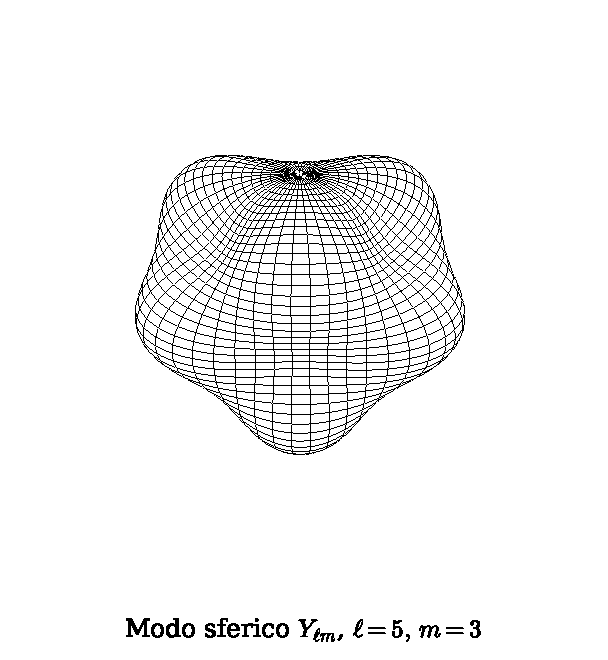
\includegraphics[width=0.5\linewidth]{modosferico53.pdf}\hfill
  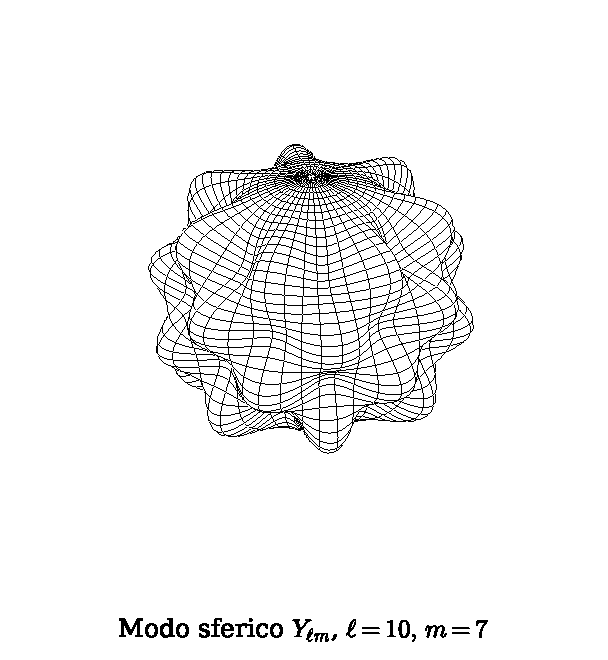
\includegraphics[width=0.5\linewidth]{modosferico107.pdf}
\end{figure}

Questa costruzione è una visualizzazione geometrica perché prende una funzione definita sulla sfera, \(Y_{\ell m}(\theta,\phi)\), che in origine è solo un numero associato a ogni direzione, e la traduce in una deformazione dello spazio tridimensionale. In pratica si passa da un oggetto astratto (una funzione su \(S^2\)) a una superficie immersa in \(\mathbb{R}^3\), dove il valore della funzione viene reinterpretato come uno spostamento radiale della sfera unitaria. Questa operazione non è contenuta nella teoria originale dei modi sferici: nell’equazione di Laplace o nella separazione delle variabili, i modi \(Y_{\ell m}\) non “spostano” la geometria, ma descrivono soltanto come varia un campo lungo le direzioni angolari. Il loro significato reale è quindi quello di modi di variazione dell’intensità del campo, cioè di basi che permettono di rappresentare qualunque dipendenza angolare di una soluzione armonica. La visualizzazione a “patata deforme” è utile perché rende immediatamente visibili due proprietà fondamentali che, nella forma astratta, sono meno intuitive: la struttura dei nodi (le regioni in cui il modo si annulla) e la distribuzione dei segni del campo (positiva o negativa). Tuttavia, è importante capire che ciò che nei grafici appare come una deformazione spaziale corrisponde, nella teoria, non a una deformazione della geometria, ma a una variazione dell’intensità del campo scalare nello spazio. In altre parole, i veri modi sferici non modificano la forma dell’oggetto su cui sono disegnati: descrivono come un campo (nel contesto fisico un potenziale ad esempio) cambi direzione per direzione. La “patata” è quindi solo un artificio visivo che trasforma una distribuzione angolare di valori in una superficie, per rendere percepibile la struttura dei modi, ma il contenuto fisico e matematico rimane quello di una funzione scalare sulla sfera.
\\
\\\underline{\textbf{Nota}}: La tecnica di visualizzazione geometrica utilizzata è la stessa che genera le forme degli orbitali atomici, che sono frutto di un'equazione differenziale dalla struttura matematica simile.



































\newpage

\chapter*{Epilogo}
\addcontentsline{toc}{chapter}{Epilogo}

Tra le persone che hanno collaborato a questo progetto desidero ringraziare il mio amico Dario, del dipartimento di ingegneria aerospaziale del POLITO, che ha realizzato i grafici dell’esempio avanzato del terzo capitolo e mi ha supportato con consigli, confronti e osservazioni durante tutta la stesura. Un ringraziamento va anche a Flavia Curina, Francesco Sermi e Federico Allegri per l’aiuto nella revisione del testo.
\\Un pensiero speciale, però, va al mio povero cane, che mi ha fatto compagnia durante le innumerevoli nottate dedicate a questo lavoro, condividendo silenziosamente ore di studio, appunti sparsi e momenti di sconforto, fino a farmi scoprire che persino gli animali possono avere le occhiaie.
\\In definitiva, spero di essere riuscito a trasmettere almeno una parte della passione che mi ha accompagnato nello studio di questa materia, una disciplina che, come spesso accade con la matematica, riesce continuamente a sorprendere e a mettere davanti a costruzioni tanto astratte quanto straordinariamente eleganti. Dietro risultati che a volte sembrano quasi irraggiungibili si nasconde infatti il lavoro di menti eccezionali, veri giganti del pensiero come D. Hilbert o J.V. Neumann, capaci di cambiare per sempre il modo di concepire la matematica e la realtà stessa.
\\Auguro infine a chiunque leggerà queste pagine di riuscire ad appassionarsi allo studio, lasciandosi guidare dalla curiosità, dal desiderio di comprendere e da quello stupore che rende ogni scoperta, grande o piccola, qualcosa di profondamente affascinante.
\\
\\
\\Filippo











































































\newpage
\addcontentsline{toc}{chapter}{Bibliografia}
\chapter*{Bibliografia}

\subsubsection{\underline{Libri di testo}}

\begin{itemize}
    \item H. Brezis: Analisi funzionale, Teoria e applicazioni
    \item Kolmogorov-Fomin: Elementi di teoria delle funzioni e di analisi funzionale
    \item B. Martelli: Geometria e algebra lineare
    \item E. Paolini: Appunti di analisi 1
    \item E. Giusti: Analisi Matematica 2
    \item M. Pedersen: Functional Analysis in Applied Mathematics and Engineering
    \item Cannarasa-D'Aprile: Introduzione alla teoria della misura e all'analisi funzionale
    \item E. Onofri: Lezioni sulla Teoria degli Operatori Lineari
    \item A. Maggi: Metodi matematici delle teorie quantistiche, volume 1: 
    \\Operatori negli spazi di Hilbert e analisi di Fourier
    \item A. Maggi: Metodi matematici delle teorie quantistiche, volume 2: 
    \\Autoaggiunzione e formulazione algebrica della meccanica quantistica \mbox{(capitoli 1, 2, 3)}
\end{itemize}

\subsubsection{\underline{Appunti e dispense}}

\begin{itemize}
    \item Bolognesi-Bracci: Metodi 1
    \item F. Sermi: Appunti di Complementi di AM 2
    \item Komornik-Loreti: Appunti di analisi matematica, l'integrale di Lebesgue
    \item A. Visintin: Serie di Fourier
    \item L.D. Marini: Complementi di Matematica
    \item Salsa-Verzini: Equazioni a Derivate Parziali, complementi ed esercizi
\end{itemize}






\end{document}